\documentclass[a4paper]{svmono}

\newboolean{two_sided} %Deklaration
\setboolean{two_sided}{true} %Zuweisung
\usepackage{type1cm}
\usepackage{makeidx}         % allows index generation
\usepackage{graphicx}        % standard LaTeX graphics tool
\usepackage{multicol}        % used for the two-column index
\usepackage[bottom]{footmisc}% places footnotes at page bottom
\usepackage{amsmath}
\usepackage{bm}
\usepackage{amssymb}
\usepackage[export]{adjustbox}
\usepackage{mathtools}
\usepackage{bbold}
\usepackage{subfigure}
\usepackage{hyperref}
\usepackage{cleveref}
\usepackage{lipsum}
\usepackage[utf8]{inputenc}
\usepackage[english]{babel}
\usepackage{pdfpages}
\ifthenelse{\boolean{two_sided}}{
    \usepackage[top=3cm,bottom=4cm,outer=2cm,inner=5cm]{geometry}
    }{
    \usepackage[top=3cm,bottom=4cm,outer=3.5cm,inner=3.5cm]{geometry}
}
\usepackage[normalem]{ulem}
\usepackage{braket}
\usepackage{tikz}
\usepackage{ifthen}
\usepackage{dsfont}
% \usepackage{microtype}
\usetikzlibrary{tikzmark}

% \interfootnotelinepenalty=10000

% % with old LaTeX-Live version
% \usepackage[backend=bibtex]{biblatex}
% \addbibresource{biblio.bib}

% with newer LaTeX-Live version
\usepackage{etoolbox}
\cslet{blx@noerroretextools}\empty
\ifthenelse{\boolean{two_sided}}{
    \usepackage[backend=bibtex,doi=false,url=false,eprint=false]{biblatex}
    }{
    \usepackage[backend=bibtex]{biblatex}
}
\addbibresource{biblio.bib}
\usepackage{autonum}

\usepackage{csquotes}

\newcommand{\todo}[1]{{\color{cyan} \scshape !!! #1 !!!}}
\newcommand{\todoil}[1]{{\color{cyan} \scshape #1}}

\setlength{\parskip}{0.2cm}

%!TEX root = thesis.tex
%%%%%%%%%%%%%%%%%%%%%
\def\ri{\mathrm i}
\def\re{\mathrm e}
\def\rd{\mathrm d}
\def\rD{\mathcal D}
\def\hc{{\rm h.c.}}
\def\tr{{\rm tr}}
\def\C{\mathcal{C}}
\def\DC{\Delta\C}
\def\GX{\Gamma X}
\def\DCav{\overline{\Delta\C}}
\def\up{\uparrow}
\def\down{\downarrow}
\def\pdag{{\vphantom\dag}}
\def\pp{\vphantom{n'}}
\def\Cav{\overline\C}
\def\MH{H}
\def\HS{\mathcal{H}}
\def\FS{\mathcal{F}}
\def\omegaT{\tilde{\omega}}
\def\tbc{{\\[1cm]\bf \color{red}[TO BE CONTINUED...]}}
\newcommand{\ave}[1]{\langle #1 \rangle}
\newcommand{\sign}[1]{\text{sign}\left( #1 \right)}
\newcommand{\commutator}[1]{\left[ #1 \right]}
\newcommand{\anticommutator}[1]{\left\{ #1 \right\}}
\newcommand{\brlr}[1]{\left( #1 \right)}
\newcommand{\abs}[1]{\left| #1 \right|}


\makeindex % used for the subject index
%%%%%%%%%%%%%%%%%%%%%%%%%%%%%%%%%%%%%%%%%%%%%%%%%%%%%%%%%%%%%%%%%%%%%%%%%%%%%%%%

\begin{document}

\author{Andreas Haller}
\title{On the tuning of particle transport,\\ strongly correlated helical phases and\\ the measurement of topological invariants}
\subtitle{Dissertation for the award of the title\\[0.5cm] {\Large``Doctor of Natural Sciences''}\\[0.5cm] at the Faculty of Physics, Mathematics and Computer Science\\ of the Johannes Gutenberg-University in Mainz}

\maketitle

\frontmatter%%%%%%%%%%%%%%%%%%%%%%%%%%%%%%%%%%%%%%%%%%%%%%%%%%%%%%%%%%%%%%%%%%%%
% \newpage
% \setcounter{page}{1}

%!TEX root = thesis.tex
%%%%%%%%%%%%%%%%%%%%%
\chapter*{Acknowledgments}
\addcontentsline{toc}{chapter}{Acknowledgments}
Now that I am right at the finish line, besides being happy that the exhaustive part is finally over, I feel a great deal of gratitude.
I would simply not have made it through, were it not for the wonderful people that take part in my life.

First of all I want to thank the members of the examination board for taking the time to evaluate the dissertation.
I know that you are all incredibly busy, and truly appreciate your tremendous effort in training the next generation of scientists.

I want to express my deep gratitude towards {\it Prof. Michele Burrello}.
You are one of the first persons I approach for professional advice, and I am always astonished by how much you know about physics.
Thank you so much for your mentoring, and for inviting me to the Niels Bohr Institute.
Brainstorming with smart and inspiring people is one of the best experiences during my PhD.
One of the best examples out of of this ``equivalence class'' of individuals is {\it Prof. Pietro Massignan}.
I am looking forward to visiting the post-pandemic Primavera Sound Festival with you and Hélia.
Most of my academic collaborators are Italian, and although I am not a fan of cliches, I must admit that they are indeed very passionate:
Thank you, {\it Michele Filippone}, for your regular motivation speeches during the time we worked together, for having me around in Geneva, for showing me the Bains des Pâquis and warning me about drinking cold water after a Swiss Fondue.
Speaking of passionate Italians, I want to express my gratitude towards {\it Jun.-Prof. Jamir Marino}.
Thank you ``für den frischen Wind'' as we Germans like to say, for your feedback regarding my thesis and for putting so much effort in a lively scientific exchange, which is incredibly hard to maintain right now.
By now it is clear to me that an academic career is unavoidably linked to a level of uncertainty: be it compensation, doubting yourself or feeling unrecognized and irrelevant, it results in a lot of unnecessary distraction from actual work.
I am grateful to the head of our group, {\it Prof. Peter van Dongen}, who managed to eliminate most of these uncertainties during the period of my PhD.
Thank you for your scientific advice, for being part of the examination board, and for carefully reading this thesis.
I am glad that you consider me part of your little ``bubble'', and I wish you the best for the future.
I want to thank {\it Prof. Patrick Windpassinger} for writing a letter of recommendation to the graduate school and for being part of the examination board.
My PhD would have been impossible without the scholarship of the Graduate School Materials Science in Mainz (MAINZ) and the Max Planck Graduate Center (MPGC).
Special thanks to {\it Michael Fuchs}, {\it Katrin Klauer}, and to {\it Prof. Thomas Speck}.

My student's life would have been pretty sad and lonely without a group of fellows: {\it Matteo Campo}, {\it Álvaro Díaz Fernández}, {\it Achim Harzheim}, {\it William Janke}, {\it Johannes Jünemann}, {\it Philipp Schmoll} and {\it Niklas Tausendpfund}.
Thank you for taking the journey with me and for reading part of this thesis.
I already miss our discussions, joint conferences, lunches and coffee breaks.

Music is a big part of my life, and it hurts me very much that these past few months were exceptionally quiet.
To all my musician friends, in particular to {\it Simon Engelhardt}, {\it Carlos Wagner} and the Grundfunk family:
There will be a time when we enjoy once more the incredible joy of playing with real people, at a real stage, and in front of an audience.
Until then, hold on tight and keep on practicing.

Sometimes (mostly Tuesdays) I came in late due to the merciless morning squash matches between me and {\it Andreas Dittinger}, {\it Fabian Kolf} and {\it Maximilian Shaikh-Yousef}.
Before my passion for squash, I was happily climbing like an ape during my free evenings in the Blockwerk Mainz with {\it Johannes} and {\it Julia Hofmann}, {\it Ruben Hoffmann} and the ``BFE crew'', which again resulted in me coming in late to university.
At other times, I overslept because of a merry wine-drinking session with our favorite upstairs neighbors {\it Laura Hollegger} and {\it Max Henderson}.
To all of my dear friends: Thanks for the joy and happiness you bring into my life.

Family always comes first, although by now we live a bit detached from each other.
I want to thank my brother-in-law, {\it Stefan Stamer}, and my parents-in-law, {\it Helma Heinz-Stamer} and {\it Thomas Stamer}.
You know me for half of my life now, and I can only imagine how annoying it must have been for you to meet me while I was a long-haired teenager.
Joking aside, I always feel warm and welcome when I am around you, and I thank you deeply for trusting me with the biggest treasure you have:
{\it Susanne}, you are the love of my life.
I don't know if you remember our chat nine years ago, but you are the reason why I pursued a career as a Physicist, which, besides marrying you, was one of the best decisions of my life.
I want to thank my grandma, {\it Irmgard Heinz}, and I hope this message reaches you somehow.
You were the sweetest person of age that I know, always happy when we passed by, and never showed your disappointed if we were busy otherwise.
I remember our joint trip to the canary islands with Susanne like it was yesterday, because it woke my curiosity to travel the world.

To my siblings, {\it Michael Haller} and {\it Astrid Fengler}.
Thank you for your patience with me.
% I've not always been the best little brother, and certainly was a rascal when I was younger.
Despite all our differences, I know that I can always count on you, and I am deeply grateful for having you in my life.
% Since my parents do not understand english, but certainly deserve one of the biggest thanks, allow me to switch languages for a while.
{\it Liebe Mama, lieber Papa}, ihr habt mein Studium stets unterstützt, auch wenn ihr keinen Bezug zu dem Thema habt.
Euch war es stets das oberste Gut, dass wir die wichtigen Entscheidungen unseres Lebens unvoreingenommen und selbstständig getroffen haben.
Nur durch dieses große Vertrauen in uns sind wir zu den Personen geworden, die wir heute sind.
Dafür liebe ich euch und bin euch unendlich dankbar.

Al mio capo {\it Prof. Matteo Rizzi}:
You made all of this possible by shaping me into the scientist I am today.
I remember very well when I entered your office for the first time, not knowing what to expect, a little shy and intimidated by your wisdom.
Although I knew so little at the time we started working together, you never lost interest and aided me to the best of your abilities.
I could not have been guided better and I am proud to call myself your student.
With all of my heart, I deeply thank you for our joint time and wish the best to you, Michela, and Giovanni.

I am grateful to everyone that shaped and decorated the path of my PhD.
It has been a wonderful experience, and I would do it all over again.

%%%%%%%%%%%%%%%%%%%%%%%%%%%%%%
%!TEX root = thesis.tex
%!TeX spellcheck = en-US,en-DE
%%%%%%%%%%%%%%%%%%%%%%%%%%%%%%
%
\chapter*{Abstract}
\addcontentsline{toc}{chapter}{Abstract}
% \thispagestyle{empty}
%
In this thesis, we investigate the effects of interactions in several different quasi one-dimensional ladder models of fermions and bosons, such as those encountered in ongoing experiments of synthetic quantum matter, in particular in setups of ultracold atoms trapped in optical lattices.

In fermionic systems, we found a possibility to flexibly tune the zero frequency component of the conductivity at zero temperature (a.k.a. the Drude weight) by repulsive density-density interactions.
The enhancement of this quantity under repulsive interactions is contradicting the ``common wisdom'' that one-dimensional systems should always show a decreasing Drude weight.
The loophole is given through the slim 2D extension of quasi one-dimensional ladders.
It allows to generate pseudospin polarized band structures which leads to the anomalous behavior of the Drude weight in interacting systems.
Our results are thus relevant for the modification of transport properties of coupled-wire systems in general.
The results are based on perturbation theory, Abelian bosonization, and numerical estimates in the non-perturbative regime through matrix product state (MPS) simulations.
% The analytic concepts necessary to comprehend this paper are illustrated in \cref{sec:periodic_potentials,sec:tight_binding_systems,sec:tomonaga_LL,sec:LL_with_spin}.
% In addition, we use matrix product state (MPS) simulations, which are presented in \cref{ch:matrix_product_states}.

We study the emergence of so-called helical liquids by repulsive interactions and density-assisted hoppings, resulting from a commensurability between particle density and flux generated from complex hopping elements.
Some of these phases have a natural extension to (fractional) Quantum Hall phases in two spatial dimensions, e.g. the Laughlin-like states, and can thus be interpreted as the predecessors of (fractional) topological phases of matter.
The study of strongly correlated helical liquids is thus important for the bottom-up fabrication of (fractional) topological phases in setups of synthetic quantum matter.
For fermions, we study the emergence of an exotic phase located at particle filling factor $\nu=1/2$ which naturally extends to a fractional Quantum Hall phase: the bosonic $K=8$ state.
We then study a similar phase in a ladder of hard-core bosons, located at filling factor $\nu=1$.
In both cases, we derive the phase diagram through renormalization group theory calculations and test our hypotheses through MPS simulations.

A natural quest in the context of topological insulators concerns the measurement of topological invariants, especially in the case of interacting systems, where a priori it does not amount to a band dispersion quantity.
For chiral symmetric systems, we propose a simple dynamical protocol based on the mean chiral displacement which provides a tomography of the topological index and indicates the presence of symmetry-broken phases through a characteristic divergence.
This protocol is tested using dynamical MPS simulations, and we provide a basic blueprint for an experiment of ultracold atoms trapped in optical lattices.


\tableofcontents

% %!TEX root = thesis.tex
%%%%%%%%%%%%%%%%%%%%%
\extrachap{Acronyms}
\begin{description}[PUTLONGEST]
    \item[ABC]{Spelled-out abbreviation and definition}
    \item[BABI]{Spelled-out abbreviation and definition}
    \item[CABR]{Spelled-out abbreviation and definition}
\end{description}

\extrachap{Definitions}
\begin{description}[PUTLONGEST]
    \item[$\MH$]{Full Hamiltonian (with interactions)}
    \item[$\MH_0$]{Kinetic Hamiltonian (tight-binding part)}
\end{description}



\mainmatter%%%%%%%%%%%%%%%%%%%%%%%%%%%%%%%%%%%%%%%%%%%%%%%%%%%%%%%%%%%%%%%%%%%%%

%%%%%%%%%%%%%%%%%%%%%%%%%%%%%%
%!TEX root = thesis.tex
%!TeX spellcheck = en-US,en-DE
%%%%%%%%%%%%%%%%%%%%%%%%%%%%%%
%
\chapter*{Introduction}
\addcontentsline{toc}{chapter}{Introduction}
%
In this thesis, we investigate the effects of interactions on several different quasi one-dimensional ladder models of fermions and bosons.
Our models are motivated from the ``building blocks'' of state-of-the-art experiments such as those employed in the framework of ultracold atoms trapped in optical lattices: complex tunneling amplitudes, diagonal cross hoppings and tunable (repulsive/attractive) interactions.

Taken the customary terminology for granted, let me start by a brief summary of the new results we established during the period of this thesis, presented in \cref{part:results}.
The analytical and numerical methods employed in our works build up on the theoretical concepts illustrated in \cref{part:theory}.

In fermionic systems, we found a possibility to flexibly tune the zero frequency component of the conductivity at zero temperature (a.k.a. the Drude weight) by repulsive density-density interactions (see \cref{drude_increased1}).
The enhancement of this quantity under repulsive interactions is contradicting the ``common wisdom'' for one-dimensional quantum which should always show a decreasing Drude weight.
The ``loophole'' is given through the slim 2D extension of our ladder, which allows to generate pseudospin polarized band structures which, ultimately, lead to the mentioned effects on the Drude weight.
Our results are therefore interesting for the modification of transport properties of coupled-wire systems in general.
The analytic concepts necessary to comprehend this paper are illustrated in \cref{sec:periodic_potentials,sec:tight_binding_systems,sec:tomonaga_LL,sec:LL_with_spin}.
In addition, we use matrix product state (MPS) simulations, which are presented in \cref{ch:matrix_product_states}.

We study the emergence of so-called helical liquids by repulsive interactions (see \cref{one_half1,integer1}) and density-assisted hoppings (see \cref{chiral1}).
In general, such phases result from a commensurability between particle density and flux, and share many similarities to the phases encountered in the Quantum Hall effect.
In this sense, some of the quasi one-dimensional helical phases can be interpreted as the predecessor of topological order, thus sometimes dubbed pre-topological, if they have a natural extension to 2D.
For fermions (see \cref{one_half1}), we study the emergence of an exotic phase located at particle filling factor $\nu=1/2$ which naturally extends to a fractional Quantum Hall phase, i.e. the bosonic $K=8$ state.
We then also study a similar phase in a ladder of hard-core bosons (see \cref{integer1}), located at filling factor $\nu=1$.
In both cases, we derive the phase diagram through renormalization group (RG) theory calculations and test our hypotheses through MPS simulations.
The introduction to the path integral formalism and RG is found in \cref{sec:properties_of_real_scalar_fields_and_their_correlations,sec:renormalization_group_theory}.

A natural quest in the context of topological insulators concerns the measurement of the topological invariant, especially in the case of interacting systems, where a priori it does not amount to a band dispersion quantity.
For chiral symmetric systems, we propose a simple dynamical protocol based on the mean chiral displacement which provides a tomography of the topological index (see \cref{mcd1}).
We furthermore provide a basic experimental blueprint in order to implement our proposition.
On the analytic side, we rely on standard band theory and test our hypotheses with MPS simulations.
The introduction to topological phases of matter in general is found in \cref{ch:topological_phases_of_matter}.

As an undergraduate student studying elementary physics, I always thought of quantum particles as plane waves living in the differential-geometric world of ``first quan\-ti\-zation'' which (at least for me) was both beautiful and frustrating at the same time as the task of solving the most simple problems may become quite involved, if not even impossible.
The modern approach is not a straightforward attempt to solve the real-space wave function by integrating a given Schrödinger equation: It rather sticks to an alternative representation in the algebraic world of ``second quantization'' where the action of operators dictates all physical consequences.
I must admit that I find the nomenclature of ``first'' and ``second'' somewhat confusing, as there is no such thing as two consecutive ways of quantization -- it's just two alternative and consistent ways of describing the same theory.
Ultimately, I've learned to accept this issue as a result of chronology: the original formulation of quantum mechanics is commonly called first quantization, in which the (motion of the) particle is quantized and possible electromagnetic fields or potentials are considered classical, whereas quantized fields have been formulated in the language of second quantization.
However, as we will see soon, the advantage of second quantization manifests itself in a simpler and more efficient way to describe many-body systems such that its development can be seen as the first major cornerstone in the emergence of quantum field theory.

Independent of the formulation, be it first or second, all quantum theories require certain basic concepts:
all quantum states are represented by state vectors $\{|q\rangle\}$ forming a complete basis of the Hilbert space and observables are defined through Hermitian operators acting on that space.
The states are given through a set of good quantum numbers $q$, e.g. for the electron of hydrogen $(n,l,m)$ associated with the total energy, angular momentum and its projection along the primary axis.

In \cref{part:theory}, I review these concepts in more detail.
The first sections, i.e. \cref{sec:creation_and_annihilation_operators,sec:representation_of_generic_operators,sec:periodic_potentials,sec:tight_binding_systems}, are aimed to guide undergraduate students which are new in the field of condensed matter.
To become familar with the basics, I review the tight binding approximation in \cref{sec:tight_binding_systems}, derived from the Kronig-Penney model in the strong potential limit (see \cref{sec:periodic_potentials}).
I then illustrate the treatment of interactions on top of a quadratic/non-interacting Hamiltonian which is a crucial tool in the understanding of quantum matter.
This becomes particularly easy in the concept of Luttinger liquids (see \cref{sec:tomonaga_LL}) as a first example of a quantum field theory satisfying the algebra of a quantum harmonic oscillator.
The key in Luttinger liquids is that the effective theory describing intrinsically interacting microscopic models remains quadratic at the operator level, and as such effectively non-interacting.
I then use the formalism of path integrals (see \cref{sec:properties_of_real_scalar_fields_and_their_correlations}) to derive analytic expressions of the correlation functions.
A common interaction which potentially melts the Luttinger liquid phase is a sine-Gordon term, which I derive in \cref{sec:LL_with_spin}.
In order to treat such higher-order interactions analytically, I introduce the concept of renormalization group theory (see \cref{sec:renormalization_group_theory}), which provides a platform to study if and when the Luttinger liquid basis must be exchanged in favor of the collective many-body basis dictated by the interactions.
One major drawback is that renormalization group theory relies on many simplifications along the way to make the calculation amendable, and microscopic details of the model are often lost in the approximations.
These details are exchanged in favor of ``universality'', an effective theory which describes the physical properties of a family of different microscopic models at long scales.
In this framework, it is thus not intended to provide quantitative predictions for the microscopic theories, such that numerical tools become essential.

A brute force calculation of a full solution scales exponentially with the number of constituents, such that exact diagonalization of interacting models is limited to small system sizes (e.g. $\sim 20$ sites for interacting spin-1/2 models in typical studies).
This stresses the need for more efficient numerical techniques in the study of non-perturbative regimes which cannot be amended analytically.
In this thesis, I mainly use matrix product states (MPS), and I illustrate the main concepts in \cref{ch:matrix_product_states}.
In \cref{sec:tensor_networks,sec:reduced_density_matrix_and_renyi_entropy}, I begin with a general introduction into the field of tensor networks and MPS.
A general discussion of scaling relations of the entanglement entropy is used to explain the effectivity of the MPS Ansatz (see \cref{sec:scaling_relations_of_the_entanglement_entropy}).
As a natural extension to MPS, I then introduce matrix product operators (MPO) in \cref{sec:matrix_product_operators} which are most useful to express the Hamiltonian, and to calculate observables in general.
After the preliminary introductions, I introduce the basic strategy to approximate ground states based on an MPS Ansatz in \cref{sec:variational_ground_state_search}.
This algorithm is quite similar to the (imaginary) time evolution presented in \cref{sec:time_evolution}, which can also be used to simulate finite temperature systems, presented in \cref{sec:finite_temperature}.
I conclude the chapter by a basic introduction into symmetry invariant MPS formulations, discussed in \cref{sec:exploiting_symmetries}.

Perhaps the most interesting behavior of quantum many-body physics is that of so-called emergent phenomena -- e.g. the appearance of quasi-particles which extend the canonical statistical properties of fermions and bosons in low dimensions, or the presence of robust quasi-particles at the boundaries of a topological insulator.
For a basic overview of this topic, I review the classification of non-interacting topological matter in \cref{ch:topological_phases_of_matter}.
The key concept for the full classification is based on topological band theory, presented in \cref{sec:topological_band_theory}, a genuinely non-interacting formulation of symmetry protected topological phases of matter.
The notion of the topological index arises from the Berry phase and the Berry connection, and I recap the original paper.
As an example, the Su-Schrieffer-Heeger chain is then explored in \cref{sec:the_SSH_chain} to apply the introduced concepts.
I conclude the third chapter by explaining the classification of topological insulators and superconductors in \cref{sec:Periodic_table_of_topological_insulators_and_superconductors}.

In \cref{part:results}, I summarize my original contributions to our published works, which are then presented in a thematic manner.
This thesis is concluded by a summary and perspectives about interesting future directions.


%!TEX root = thesis.tex
%%%%%%%%%%%%%%%%%%%%%

\begin{partbacktext}
    \part{Theoretical Prerequisites}
    \label{part:theory}
\end{partbacktext}

%!TEX root = thesis.tex
%%%%%%%%%%%%%%%%%%%%%%%
\chapter{The quantization of motion and fields}
\label{ch:the_quantization_of_motion_and_fields}
The present chapter is inspired by a number of excellent books and lectures such as~\cite{AshcroftMermin1978,AltlandSimons2010,BruusFlensberg2004,Czycholl2016,FetterWalecka2003,Giamarchi2003,Rizzi2016,Burrello2020} extending the basic aspects of quantum mechanics to a modern way of understanding quantum field theory in general.
%
%
%%%%%%%%%%%%%%%%%%%%%%%%%%%%%%%%%%%%%%%%%%%%%%%%
\section{Creation and annihilation operators}
\label{sec:creation_and_annihilation_operators}
%%%%%%%%%%%%%%%%%%%%%%%%%%%%%%%%%%%%%%%%%%%%%%%%
%
%
Consider a complete set of quantum numbers $\{\alpha\}$ which label a normalized set of states $\{\ket{\alpha}\}$ spanning the full Hilbert space $\HS^1$ of a generic single particle system described by the (time-independent) Schrödinger equation
\begin{align}
    \hat H \ket{\alpha} = \varepsilon_\alpha\ket{\alpha}.
\end{align}
The single particle wave function $\Psi_\alpha(r)$ of a quantum state occupying $\alpha$ is defined as the inner product of the vector $\ket{\alpha}$ with the real-space covector, i.e.
\begin{align}
    \Psi_\alpha(r) \coloneqq \braket{r|\alpha}.
\end{align}
% \todoil{Comment already on the overcompleteness of the $r$-states, or not?}
It is is thus understood as the coefficients for the basis transform $\ket{\alpha}\rightarrow\ket{r}$, i.e.
\begin{align}
    \ket{\alpha} = \int{\rm d}{r}\, \Psi_\alpha(r) \ket{r}.
\end{align}
According to the basic postulate of quantum mechanics, the wave function of two indistinguishable particles with quantum numbers $\alpha_1$ and $\alpha_2$ is given by the (anti-) symmetrized product
\begin{align}
    \Psi_{\alpha_1,\alpha_2,\nu}(r_1,r_2) = \frac1{\sqrt2}\left(\braket{r_1|\alpha_1}\braket{r_2|\alpha_2} + \nu\braket{r_2|\alpha_1}\braket{r_1|\alpha_2}\right),
\end{align}
depending on the particle statistics upon exchange of their position, i.e. $\nu=\pm1$ for bosons and fermions, respectively.
The two-particle wave function can thus be represented by a more simple inner product
\begin{align}
    \Psi_{\alpha_1,\alpha_2,\nu}(r_1,r_2) = \left(\bra{r_1}\otimes\bra{r_2}\right)\ket{\alpha_1 \alpha_2}_\nu
\end{align}
which is given by the (anti-) symmetric Kronecker product
\begin{align}
    \ket{\alpha_1 \alpha_2}_\nu = \frac1{\sqrt2}\left(\ket{\alpha_1}\otimes\ket{\alpha_2} + \nu\ket{\alpha_2}\otimes\ket{\alpha_1}\right).
\end{align}
In general, the symmetric $N$-particle state vector is an element of the $N$-particle Hilbert space $\HS^N = \bigotimes_{i=1}^N\HS^1$ and reads
\begin{align}
    \ket{\alpha_1,\alpha_2,\dots,\alpha_N}_\nu = \frac1{\sqrt{N!\prod_{\alpha}(n_\alpha!)}}\sum_P \nu^{(1-\sign{P})/2}\ket{\alpha_{P(1)}}\otimes\ket{\alpha_{P(2)}}\otimes\dots\otimes\ket{\alpha_{P(N)}}.
    \label{eq:symmetric_many_body_state}
\end{align}
In the above equation, we assume ordered quantum numbers (e.g. increasing positions along a wire, or increasing energies), denote the total number of particles with quantum number $\alpha$ as $n_\alpha$ and $\sign{P}$ the sign of the permutation $P\in S^N$ of the permutation group [$\sign{P}=\pm1$ if the permutation is even/odd].

The representation in the ordered expression of \cref{eq:symmetric_many_body_state} is not particularly compact since equal values of $\alpha$ may appear $n_\alpha$ times in the $N$-letter long ket -- the occupation number representation removes this redundancy.
The states in this representation are then given by
\begin{align}
    \ket{n_1, n_2, \dots}_\nu = \ket{\underbrace{\alpha_1,\alpha_1,\dots,\alpha_1}_{n_1}, \underbrace{\alpha_2, \alpha_2,\dots, \alpha_2}_{n_2}, \alpha_3, \dots}
\end{align}
and they span the space $\FS^N$ of the (anti-) symmetrized $N$-particle states $\sum_{i} n_i = N$.
Thus, the subset $\FS^N\subset \HS^N$ contains all $N$-particle states which transform according to the basic postulate of quantum mechanics such that any physical state $\ket{\Psi}\in\HS^N$ can be written as a linear superposition of the Fock states
\begin{align}
    \ket{\Psi}_\nu = \sum_{\sum_i n_i = N}C(n_1,n_2,\dots)\ket{n_1,n_2,\dots}_\nu.
\end{align}
The full Fock space $\FS$ is defined as a direct sum of vector spaces with fixed $N$, i.e.
\begin{align}
    \FS = \bigoplus_{N=0}^\infty \FS^N,
\end{align}
including the one-dimensional vacuum space commonly denoted by $\{\ket{0}\}=\FS^0$.

Let us now impose a linear map $\hat a^\dag_i:\FS\rightarrow\FS$ connecting the individual subsets through
\begin{align}
    \hat a^\dag_i\ket{n_1,\dots,n_i,\dots}_\nu = \sqrt{n_i+1}\nu^{\sum_{j<i}n_j}\ket{n_1,\dots,n_i+1,\dots}_\nu
    \label{eq:creation}
\end{align}
in which fermionic states must be understood ${\rm mod}_2$ such that the Pauli exclusion principle is explicitly satisfied: $\hat a^\dag{}^2\ket{0}=\hat a^\dag\ket{1}={\rm mod}_2(1+1)\ket{{\rm mod}_2(1+1)} = 0\ket{0} = 0$.
Notice that through the linear map we can express the canonical basis of any subset $\FS^N\subset\FS$ as
\begin{align}
    \ket{n_1,n_2,\dots}_\nu = \prod_i\frac1{\sqrt{n_i!}}\left(\hat a^\dag_i\right)^{n_i}\ket{0}_\nu,
    \label{eq:Fock_basis}
\end{align}
and as such have a tool which promotes the vacuum to any state of the full Fock space.
\begin{figure}
    \centering
    \subfigure[]{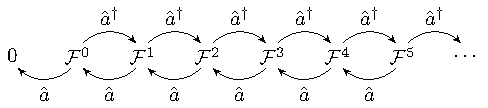
\includegraphics{figures/connected_fock_space_bosons.pdf}}
    \hfil
    \subfigure[]{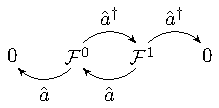
\includegraphics{figures/connected_fock_space_fermions.pdf}}
    \caption{(a) Subspaces $\FS^N$ of $N$-particle bosonic states $\ket{N}$ characterized by a single quantum number. Adjacent spaces are connected through the linear maps $a^{(\dag)}$ defined in \cref{eq:creation,eq:annihilation}. (b) Subspaces for a fermionic system characterized by a single quantum number.}
    \label{fig:fock_spaces}
\end{figure}
Notice the absence of the phase $\nu$ on the right hand side which is due to the fact that the product is ordered.
For this reason (and in the following), the linear maps $\hat a^\dag_i$ are commonly called creation operators.
Two different linear maps $j<i$ satisfy the following equation
\begin{align}
    \hat a^\dag_i \hat a^\dag_j\ket{n_1,n_2,\dots}_\nu = \nu \hat a^\dag_j\hat a^\dag_i\ket{n_1,n_2,\dots}_\nu,
\end{align}
and thus span the famous (anti-)commutation relation
\begin{align}
    \commutator{\hat a^\dag_i, \hat a^\dag_j}_\nu \coloneqq \hat a^\dag_i \hat a^\dag_j - \nu \hat a^\dag_j \hat a^\dag_i = 0.
\end{align}
From the Hermitian adjoint of the equations before we get the condition
\begin{align}
   \braket{n_1,\dots,n_i,\dots | \hat a^\pdag_i | m_1, \dots, m_i,\dots}_\nu =
   \sqrt{n_i+1}\nu^{\sum_{j<i}n_j} \delta_{n_1,m_1}\dots\delta_{n_i+1,m_i}\dots
\end{align}
and thus
\begin{align}
   \hat a^\pdag_i \ket{n_1, \dots, n_i,\dots}_\nu =
   \sqrt{n_i}\nu^{\sum_{j<i}n_j} \ket{n_1, \dots, n_i-1,\dots}_\nu,
   \label{eq:annihilation}
\end{align}
from which we obtain the algebra relations of the creation/annihilation operators
\begin{align}
    \commutator{\hat a^\pdag_i,\hat a^\dag_j}_\nu = \delta_{i,j},
    \quad
    \commutator{\hat a^\pdag_i,\hat a^\pdag_j}_\nu = 0,
    \quad
    \commutator{\hat a^\dag_i,\hat a^\dag_j}_\nu = 0.
    \label{eq:Heisenberg_algebra}
\end{align}
In reverse,~\cref{eq:Fock_basis} is a consequence of the Stone-von Neumann theorem which states that, given the Heisenberg algebra defined through~\cref{eq:Heisenberg_algebra}, the action of the operators and the representation of the Fock basis is unique (up to unitary transformations)~\cite{Hall2013}.

To conclude this first section, a change of basis $\{\ket\alpha\}\rightarrow\{\ket\beta\}$ yields\footnote{Remember that $\mathbb1 = \sum_\alpha\ket{\alpha}\bra{\alpha}$, $\ket{\beta} = \sum_\alpha\ket{\alpha}\braket{\alpha|\beta}$ and $\ket{\beta}=\hat a^\dag_\beta\ket{0}$, leading to \cref{eq:creation_annihilation_basis_rotation}.} a unitary transformation of the operators
\begin{align}
    \hat a^\dag_\beta = \sum_\alpha \braket{\alpha|\beta}\hat a^\dag_\alpha,
    \quad
    \hat a^\pdag_\beta = \sum_\alpha \braket{\beta|\alpha}\hat a^\pdag_\alpha
    \label{eq:creation_annihilation_basis_rotation}
\end{align}
which requires only a computation of the single-particle matrix elements $\braket{\alpha|\beta}$.
Before we move on to the representation of observables, a word on common notations: Quite often the authors assume a certain particle statistics and operator algebra at the beginning of their work which implies a constant (and thus dropped) subscript $\nu$.
Fermionic annihilation operators are mostly identified through the letter $\hat c$ whereas $\hat b$ often corresponds to bosonic operators.
Furthermore, a common convention identifies the commutator through crotchets
\begin{align}
    \left[\hat A,\hat B\right]\coloneqq\commutator{\hat A,\hat B}_+ = \hat A\hat B - \hat B\hat A
\end{align}
and the anticommutator through curly braces
\begin{align}
    \anticommutator{\hat A,\hat B}\coloneqq\commutator{\hat A,\hat B}_- = \hat A\hat B + \hat B\hat A.
\end{align}
Let me also provide a useful expression to evaluate the commutation relation of operator products recursively
\begin{align}
    \commutator{\hat A, \hat B \hat C}_\pm
    &= \hat A\hat B\hat C \mp \hat B\hat C\hat A + \hat B\hat A\hat C - \hat B\hat A\hat C
    \\
    &= \commutator{\hat A, \hat B}_\pm\hat C \mp \hat B\hat C\hat A \pm \hat B\hat A\hat C
    = \commutator{\hat A, \hat B}_\pm\hat C \mp \hat B\commutator{\hat A,\hat C}.
    \label{eq:recursive_commutation}
\end{align}
In many cases, the sets of quantum numbers are continuous (e.g. position $x$) and as such a sum in \cref{eq:creation_annihilation_basis_rotation} is promoted to an integral expression:
\begin{align}
    \hat a(x) = \sum_\alpha \braket{x | \alpha} \hat a_\alpha,
    \quad
    \hat a_\alpha = \int{\rd x} \braket{\alpha | x} \hat a(x).
\end{align}
This is commonly highlighted through a bracket notation of the continuous quantum number.
In conclusion, using the Fock state representation automatically assures the (anti-)symmetric properties of many-body quantum states in real space.
It provides thus an ideal basis for analytical and numerical simulations of many-body states of matter.
%
%
%%%%%%%%%%%%%%%%%%%%%%%%%%%%%%%%%%%%%%%%%%%%%%%
\section{Representation of generic operators}
\label{sec:representation_of_generic_operators}
%%%%%%%%%%%%%%%%%%%%%%%%%%%%%%%%%%%%%%%%%%%%%%%
Let us start with a general operator acting on a single particle of the full $N$-particle state (usually dubbed ``one-body operator'').
Familiar examples are the momentum or the position operator $\hat x_i$, $\hat p_i$ acting on the $i$th particle, or compositions of these operators like single particle potentials $\hat V(\hat x_i)$.
It is thus not surprising that the general expression of such operators can be given in terms of the particle creation and annihilation operators we introduced in \cref{sec:creation_and_annihilation_operators}.

A one-body operator $\hat o$ diagonal in an arbitrary single-particle basis $\{\alpha_1\}$ ($\hat o = \sum_{\alpha_1} o_{\alpha_1}\ket{\alpha_1}\bra{\alpha_1}$) is trivially extended to the $N$-particle states written in the same basis
\begin{align}
    \hat O_1
    = \sum_{\alpha_i} o_{\alpha_i}\hat a^\dag_{\alpha_i}\hat a^\pdag_{\alpha_i}.
\end{align}
This is most easily understood: one-body operators act on only a single entity of the full set of particles, leaving the others untouched.
In the diagonal basis of $\hat O_1$, the action of $\hat n_{\alpha_i}\coloneqq \hat a^\dag_{\alpha_i}\hat a^\pdag_{\alpha_i}$ just counts the number of particles in the state $\alpha_i$, which is then multiplied with the expectation value of the single-particle operator.
In a more general basis, the one-body operator transforms according to \cref{eq:creation_annihilation_basis_rotation} resulting in
\begin{align}
    \hat O_1 = \sum_{\alpha, \beta}\braket{\alpha | \hat o | \beta} \hat a^\dag_\alpha \hat a^\pdag_\beta = \sum_{\alpha,\beta}o_{\alpha,\beta}\hat a^\dag_\alpha \hat a^\pdag_\beta.
    \label{eq:one_body_operator}
\end{align}
Note that in the above, the indices $\alpha$ and $\beta$ denote a full set of quantum numbers of the many-body system.
It is now straightforward to introduce generic two-body operators $\hat O_2$,
\begin{align}
    \hat O_2 = \sum_{\alpha,\beta,\gamma,\delta}O_{\alpha,\beta,\gamma,\delta}\hat a^\dag_\alpha \hat a^\dag_\beta \hat a^\pdag_\gamma \hat a^\pdag_\delta,
\end{align}
in which the expectation value reads $O_{\alpha,\beta,\gamma,\delta}\coloneqq \braket{\alpha,\beta | \hat o | \gamma,\delta}$.
For example, a generic two-point interaction $\hat V\ket{r_1,\dots,r_N}=1/2\sum_{n\neq m}V(r_n-r_m)\ket{r_1,\dots,r_N}$ in continuous space takes the second quantized form
\begin{align}
    \hat V = \frac12\int{\rd^d r}\int{\rd^d r'}V({\bm r}-{\bm r'})\hat a^\dag({\bm r})\hat a^\dag({\bm r'})\hat a^\pdag({\bm r'})\hat a^\pdag({\bm r}).
    \label{eq:two_point_interaction}
\end{align}
The generalization to generic $M$-body operators is now straightforward
\begin{align}
    \hat O_M = \sum_{\alpha_1,\dots,\alpha_M}\sum_{\beta_1,\dots,\beta_M}O_{\alpha_1,\dots,\alpha_M,\beta_1,\dots,\beta_M}\hat a^\dag_{\alpha_1}\dots \hat a^\dag_{\alpha_M}\hat a^\pdag_{\beta_1}\dots \hat a^\pdag_{\beta_M}.
\end{align}
%
%
%%%%%%%%%%%%%%%%%%%%%%%%%%%%%%%%
\section{Periodic potentials}
\label{sec:periodic_potentials}
%%%%%%%%%%%%%%%%%%%%%%%%%%%%%%%%
To really see when second quantization becomes useful, I go one step back and review basic properties of a single particle moving in a periodic potential which is effectively characterized by a Hamiltonian composed of generic one-body operators of the form of \cref{eq:one_body_operator}.
In particular, the Hamiltonian considered here reads
\begin{align}
    \hat H_0 = \int\rd^d r\, \hat a^\dag({\bm r})\brlr{\frac{\hat{\bm p}^2}{2m}+V_{ae}({\bm r})}\hat a^\pdag({\bm r})
\end{align}
% and later impose generic two-body interactions
% \begin{align}
%     \hat V_{ee} = \frac12\sum_{s,s'}\int\rd^dr\int\rd^dr'\,V_{ee}({\bm r}-{\bm r'})a^\dag_s({\bm r})a^\dag_{s'}({\bm r'})a^\pdag_{s'}({\bm r}')a^\pdag_{s}({\bm r})
% \end{align}
with operators $\hat a^\pdag({\bm r})$ annihilating a particle at position $\bm r$.
The local potential $V_{ae}$ is a collection of $N_a$ local potentials
\begin{align}
    V_{ae}({\bm r}) = \sum_{i=1}^{N_a}v_{ae}({\bm R}_i - {\bm r})
\end{align}
and the value of $v_{ae}$ is determined by the relative distance from the position ${\bm R}_i$.
If the creation operators satisfy the anticommutator algebra in real space
\begin{align}
    \anticommutator{\hat a^\pdag({\bm r}),\hat a^\dag({\bm r'})}=\delta({\bm r}-{\bm r'}),
\end{align}
the Hamiltonian defines a spinless fermionic system embedded in an arbitrary lattice.
A regular (Bravais) lattice structure in $d$ dimensions is in general spanned by $d$ linearly independent (not necessary mutually perpendicular and normalized) vectors ${\bm x}_i$ and can thus be defined as the set
\begin{align}
    \mathcal{R} = \anticommutator{\sum_{i=1}^d n_i {\bm x}_i,\ n_i\in\mathds Z}.
\end{align}
Additional vectors $\{{\bm b}_i\}$ (sometimes called the basis) are used to define the position of the potential minima relative to the points of the Bravais lattice, such that every position in the primitive cell is given by ${\bm R}_j = \sum_i n_i {\bm x}_i + {\bm b}_j$ with integers $n_i\in\mathds Z$.
The beauty of this approach becomes visible as soon as we define the lattice translation operator
\begin{align}
    \hat T_{\bm n} : \psi_\alpha({\bm r}) \mapsto \psi_\alpha\brlr{{\bm r}+T_{\bm n}},\ T_{\bm n}\coloneqq\sum_i n_i {\bm x}_i={\bm n}\underline{\bm x}
\end{align}
which translates every function from one position to a distance parametrized through the $d$-dimensional vector ${\bm n}\in\mathds Z^d$ and the collection of all lattice vectors $\underline{\bm x}\coloneqq ({\bm x}_1,\dots,{\bm x}_d)^T$.
The local potential $V_{ae}({\bm r})$ is by definition invariant under lattice translations, and two-body interactions $V({\bm r}-{\bm r'})$ are clearly invariant under continuous translations, such that the full Hamiltonian $\hat H$ commutes with the translation operator and we can write the eigenfunctions of $\hat H$ as eigenfunctions of $\hat T_{\bm n}$.
The eigenfunctions of all translation operators $\hat T_{\bm n}$ are called Bloch waves and have the following properties\footnote{Note here that a further restriction on the values of the vector ${\bm k}$ arise from imposing boundary conditions. For instance, Born-von Karman boundary conditions imply a periodicity after $L_j$ unit translations $\psi_\alpha({\bm r}+ L_j{\bm R}_j)=\psi_\alpha({\bm r})$, which confines the allowed values of $k_j$ to integer multiples of $\frac{\bm G_j}{L_j}$ in which $\bm G_j$ is the reciprocal vector of ${\bm R}_j$, i.e. ${\bm G}_j {\bm R}_j = 2\pi/a$.}
\begin{align}
    \hat T_{\bm n}\psi_{\alpha}({\bm r}) &= c_{\bm n}\psi_{\alpha}({\bm r})\\
    c_{{\bm n}_1}c_{{\bm n}_2} &= c_{{\bm n}_1+{\bm n}_2} \Rightarrow c_{\bm n} = \re^{{\bm s}\cdot{\bm n}\underline{\bm x}},\ {\bm s}\in\mathds C^d\\
    1=\int_V\rd^dr\,\abs{\psi_{\alpha}({\bm r})}^2 &= \int_V\rd^dr\,\abs{\hat T_{\bm n}\psi_{\alpha}({\bm r})}^2 \Rightarrow 1=\abs{c_{\bm n}}^2 \Rightarrow {\bm s}=\ri{\bm k},\ {\bm k}\in\mathds R^d
\end{align}
It is now possible to phrase Bloch's theorem~\cite{Bloch1929}, which states that the eigenfunctions of a particle moving in periodic potentials assume the simple structure
\begin{align}
    \psi_\alpha({\bm r}) = \psi_{\alpha{\bm k}}({\bm r}) = \re^{\ri{\bm k}\cdot {\bm r}}u_{\alpha{\bm k}}({\bm r}).
    \label{eq:bloch_theorem}
\end{align}
Note that we introduced the translation operators eigenvalue argument $\bm k$ in the list of good quantum numbers.
In particular, $\psi$ is a weighted plane wave in which $u$ inherits the lattice periodicity
\begin{align}
    \hat T_{\bm n} u_{\alpha{\bm k}}({\bm r})
    =
    \re^{-\ri{\bm k}\cdot \brlr{{\bm r}+{\bm n}\underline{\bm x}}}c_{\bm n}\psi_{\alpha{\bm k}}({\bm r})
    =
    \re^{-\ri{\bm k}\cdot {\bm r}}\re^{-\ri{\bm k}\cdot {\bm n}\underline{\bm x}}\re^{\ri{\bm k}\cdot {\bm n}\underline{\bm x}}\psi_{\alpha{\bm k}}({\bm r})
    =
    u_{\alpha{\bm k}}({\bm r}).
\end{align}
% The particular expression of the weights obviously depends on the potential, and obtaining general solutions becomes a hard task even for simple problems\footnote{Except maybe the trivial scenario $V_{ae}({\bm r})={\rm const.}$ which implies $u=1$ in \cref{eq:bloch_theorem}.}.
In general, the wave vector $\bm k$ seems to play the same role as the particle momentum $\bm p$ in the Sommerfeld theory of a free particle.
However, this is not true as is clear from the momentum operator being $\hat{\bm p}=-\ri\hbar\bm \nabla$, and as such
\begin{align}
  \hat{\bm p}\psi_{\alpha{\bm k}}({\bm r}) = \hbar{\bm k}\psi_{\alpha{\bm k}} - \ri\hbar\re^{\ri{\bm k}{\bm r}}\bm\nabla u_{\alpha \bm k}(\bm r).
\end{align}
The vector ${\bm k}$ is thus dubbed crystal momentum, remembering the fact that $\psi_{\alpha{\bm k}}$ is only an eigenstate of momentum if the potential is constant and thus $\bm\nabla V_{ae}=0$.

As we will see in the next section, the Bloch waves can be used to define a complete set of tightly localized ``Wannier'' states, which allows to work with effective ``tight binding approximations'' in which the coupling parameters of the model are implicitly defined through overlap integrals of the Bloch functions.
This way, the many-body phases of the effective model can be studied in a more efficient way without the explicit knowledge of the coupling constants.
Nonetheless, to get an idea of the form of the Bloch functions, let us solve the Schrödinger equation of a particle moving along one dimension in the potential
\begin{align}
    V_{ae}(x) = V_0 \Theta\brlr{b-{\rm mod}_{a}\commutator{x+b}},\ V_0,a,b\in\mathds R_+
    \label{eq:kronig_penney_potential}
\end{align}
such that the nontrivial contours are of size $b$ and displaced by a factor $a$ called the lattice spacing.
This model is called the Kronig-Penney model~\cite{KronigPenney1931} and provides analytic solutions of bound electrons in the limit $b\rightarrow0$ and $V_0\rightarrow\infty$ such that $bV_0={\rm const.}$, which is depicted in \cref{fig:kronig_penney_potential}.
\begin{figure}
    \centering
    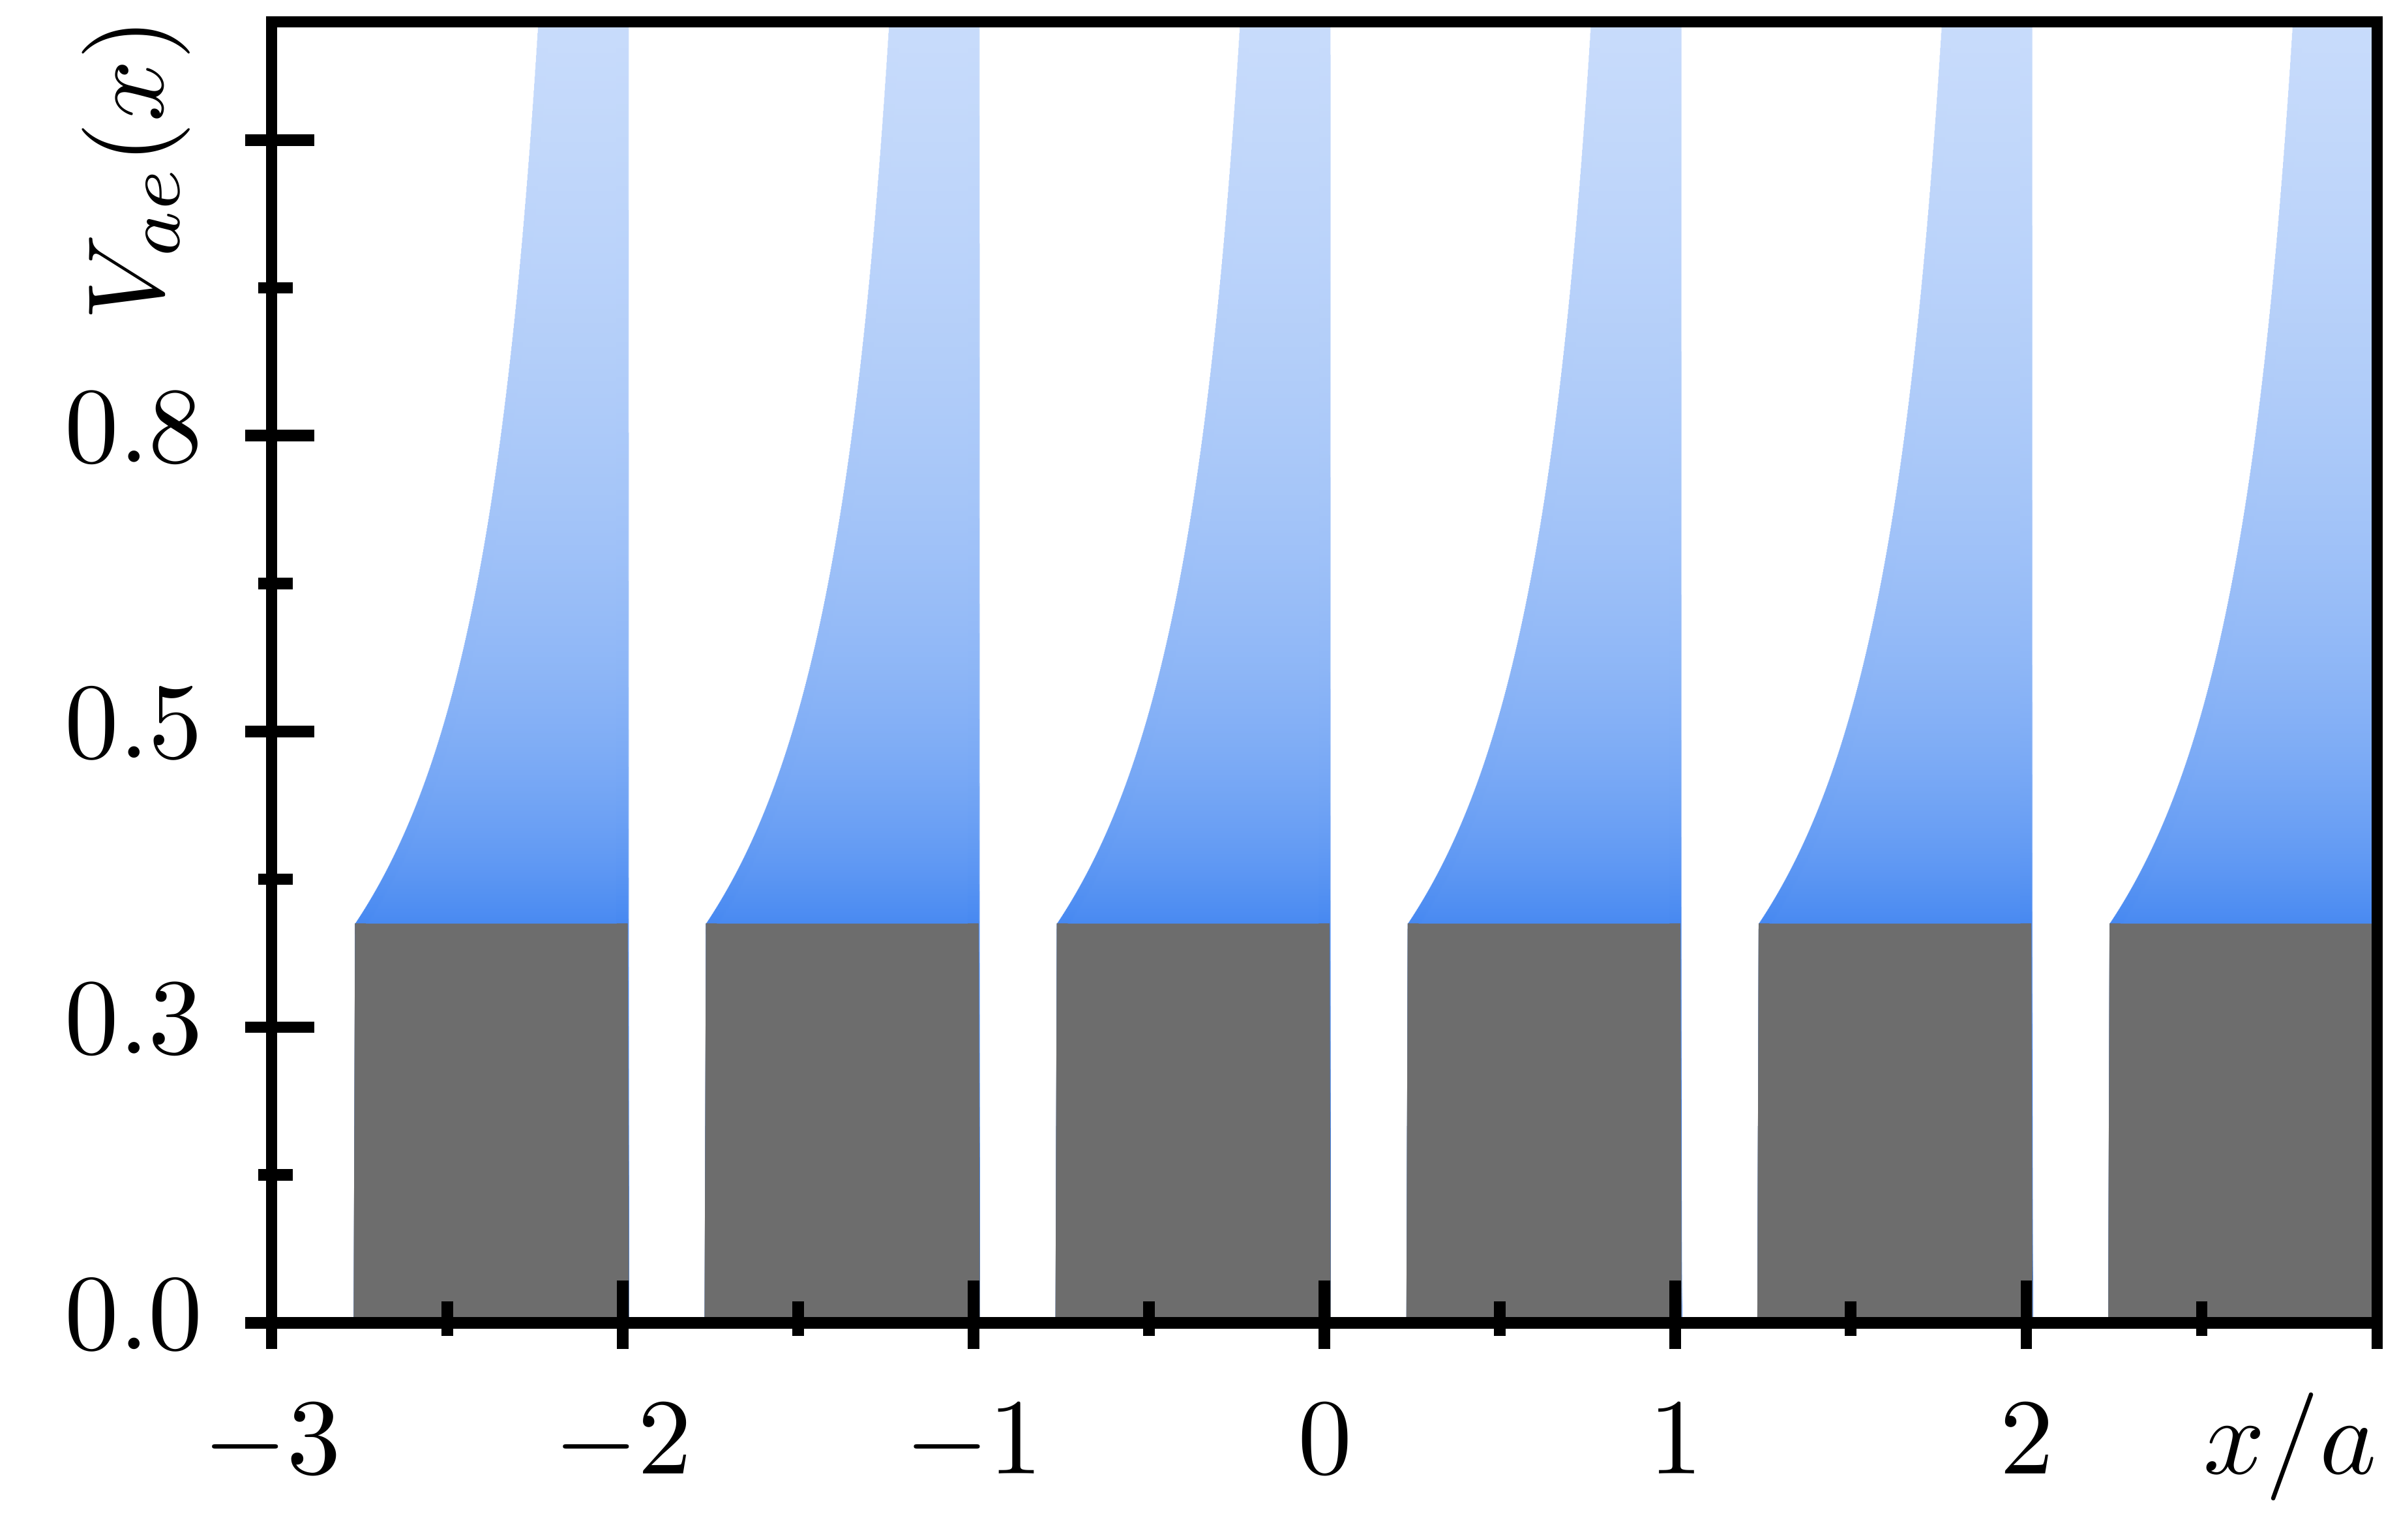
\includegraphics{figures/kronig_penney_potential.png}
    \caption{Different contours of the periodic potential \cref{eq:kronig_penney_potential} for $bV_0=1/4$. The gray boxes corresponds to the fixed values $V_0=1/3$ and $b=3/4$, while the blue gradient visualizes the limit $b\rightarrow0$ and $V_0\rightarrow\infty$ while preserving the product $bV_0=P$.}
    \label{fig:kronig_penney_potential}
\end{figure}

% In order to preserve the periodicity of the potential, the system size must be commensurate to the lattice spacing $a$, i.e. $L\in a\mathds N$.
To simplify our problem, we can consider two different regions, i.e. (i) a free particle $-\frac{\hbar^2}{2m}\partial_x^2\psi_{\rm (i)}(x) = E\psi_{\rm (i)}(x)$ and (ii) a particle moving in a constant potential $-\frac{\hbar^2}{2m}\partial_x^2\psi_{\rm (ii)}(x) = (E-V_0)\psi_{\rm (ii)}(x)$.
In order to read out the Bloch weights I conveniently factor a crystal momentum from the wave function
\begin{align}
    \psi_{\alpha k}^{\rm (i)}(x) = \re^{\ri kx}u_{\alpha k}^{\rm (i)}(x),
    \
    \psi_{\beta k}^{\rm (ii)}(x) = \re^{\ri kx}u_{\beta k}^{\rm (ii)}(x),
    \\
    u_{\alpha k}^{\rm (i)}(x) = A\re^{(\tau\alpha-\ri k) x} + A'\re^{-(\tau\alpha+\ri k) x},
    \
    u_{\beta k}^{\rm (ii)}(x) = B\re^{(\tau'\beta-\ri k) x} + B'\re^{-(\tau'\beta+\ri k) x},
\end{align}
with $\hbar^2\alpha^2 = 2m\abs{E}$, $\hbar^2\beta^2 = 2m\abs{(E-V_0)}$, $\tau^2=-\sign{E}$ and $\tau'^2=-\sign{E-V_0}$.
Plane waves are thus obtained in case of $\tau=\tau'=\ri$ are obtained for $E>V_0$.
The wave functions are supposed to be smooth at the boundaries\footnote{I hereby use the notation of limits from above or below, i.e. $f(0^\pm)=\lim_{\epsilon\rightarrow0}f(\pm\epsilon)$ for $\epsilon>0$.}, which results in
\begin{align}
    % \psi_{\alpha k}^{\rm (i)}(0^+)=\psi_{\beta k}^{\rm (ii)}(0^-),
    % \quad
    % {\psi_{\alpha k}^{\rm (i)}}'(0^+)={\psi_{\beta k}^{\rm (ii)}}'(0^-),
    % \\
    \psi_{\alpha k}^{\rm (i)}(-b+0^-)=\psi_{\beta k}^{\rm (ii)}(-b+0^+),
    \quad
    {\psi_{\alpha k}^{\rm (i)}}'(-b+0^-)={\psi_{\beta k}^{\rm (ii)}}'(-b+0^+),
\end{align}
and the Bloch functions inherit the potential's periodicity
\begin{align}
    u_{\alpha k}^{\rm (i)}(a+0^+) = u_{\alpha k}^{\rm (ii)}(0^-),
    \quad
    u_{\alpha k}^{\rm (i)}{}'(a+0^+) = u_{\alpha k}^{\rm (ii)}{}'(0^-).
\end{align}
In summary, the following matrix equation is derived
\begin{align}
    &\qquad M =\\
    &\begin{pmatrix}
        1 & 1 & -1 & -1\\
        %
        \tau\alpha & -\tau\alpha & -\tau'\beta & \tau'\beta\\
        %
        \re^{(\tau \alpha-\ri k)(a-b)}  & \re^{-(\tau \alpha+\ri k) (a-b)} &
        -\re^{-(\tau'\beta -\ri k)b}     & -\re^{ (\tau'\beta+\ri k)b} \\
        %
        (\tau \alpha-\ri k)\re^{(\tau \alpha-\ri k)(a-b)}  & -(\tau \alpha+\ri k)\re^{-(\tau \alpha+\ri k) (a-b)} &
        -(\tau'\beta -\ri k)\re^{-(\tau'\beta -\ri k)b}     & (\tau'\beta+\ri k)\re^{ (\tau'\beta+\ri k)b} \nonumber\\
    \end{pmatrix},
\end{align}
satisfying $M(A,A',B,B')^T=0$.
For nontrivial results, the determinant of $M$ should be equal to zero, which is satisfied for solutions of the transcendental equation
\begin{align}
    \cos(ka)
    =
    \cosh(\alpha\tau(a-b))\cosh(b\beta\tau')
    +
    \frac{\alpha^2\tau^2+\beta^2\tau'^2}{2\alpha\beta\tau\tau'}\sinh(\alpha\tau(a-b))\sinh(b\beta\tau).
    \label{eq:kronig_penney_transcendental_equation}
\end{align}
To approximate the right hand side in the aforementioned limits, application of
\begin{align}
    b\rightarrow0,
    \quad
    V_0\rightarrow\infty,
    \quad
    bV_0 = {\rm const.}
    \\
    \Rightarrow
    b\beta^2\rightarrow 2mbV_0/\hbar^2,
    \quad
    \cosh(b\beta\tau')\rightarrow 1,
    \quad
    \sinh(b\beta\tau')\rightarrow b\beta\tau'
\end{align}
provides an exact rewriting of \cref{eq:kronig_penney_transcendental_equation} in the limit of narrow and strong periodic potentials\footnote{This limit is actually equivalent to a potential composed by delta-distributions.}
\begin{align}
    f(\alpha a) \coloneqq \cosh(\alpha\tau a) + \tau'^2\frac{P}{\alpha\tau a}\sinh(\alpha\tau a),
    \quad
    P \coloneqq mabV_0/\hbar^2.
    \label{eq:kronig_penney_transcendental_equation_approx}
\end{align}
If we assume bound states between the potential wells $0<E<V_0$, the signs become $\tau^2=-1$ and $\tau'^2=+1$, such that \cref{eq:kronig_penney_transcendental_equation_approx} evaluates to
\begin{align}
    f(\alpha a) = \cos(\alpha a) + \frac{P}{\alpha a}\sin(\alpha a).
    \label{eq:kronig_penney_transcendental_equation_approx_bound}
\end{align}
For nonzero $P$, the right-hand-side of \cref{eq:kronig_penney_transcendental_equation_approx_bound} is not bound to the interval $[-1,+1]$ spanned by the left-hand-side of \cref{eq:kronig_penney_transcendental_equation}, and establishes values of $\alpha$ (thus, the square-root of the energy $E$) for which no (real) momentum exists (see \cref{fig:kronig_penney_dispersion} (a)).
Such energies are called forbidden and allow for a first understanding of band-gaps induced by the nonzero lattice potential $V_0>0$.
\begin{figure}
    \centering
    \subfigure[]{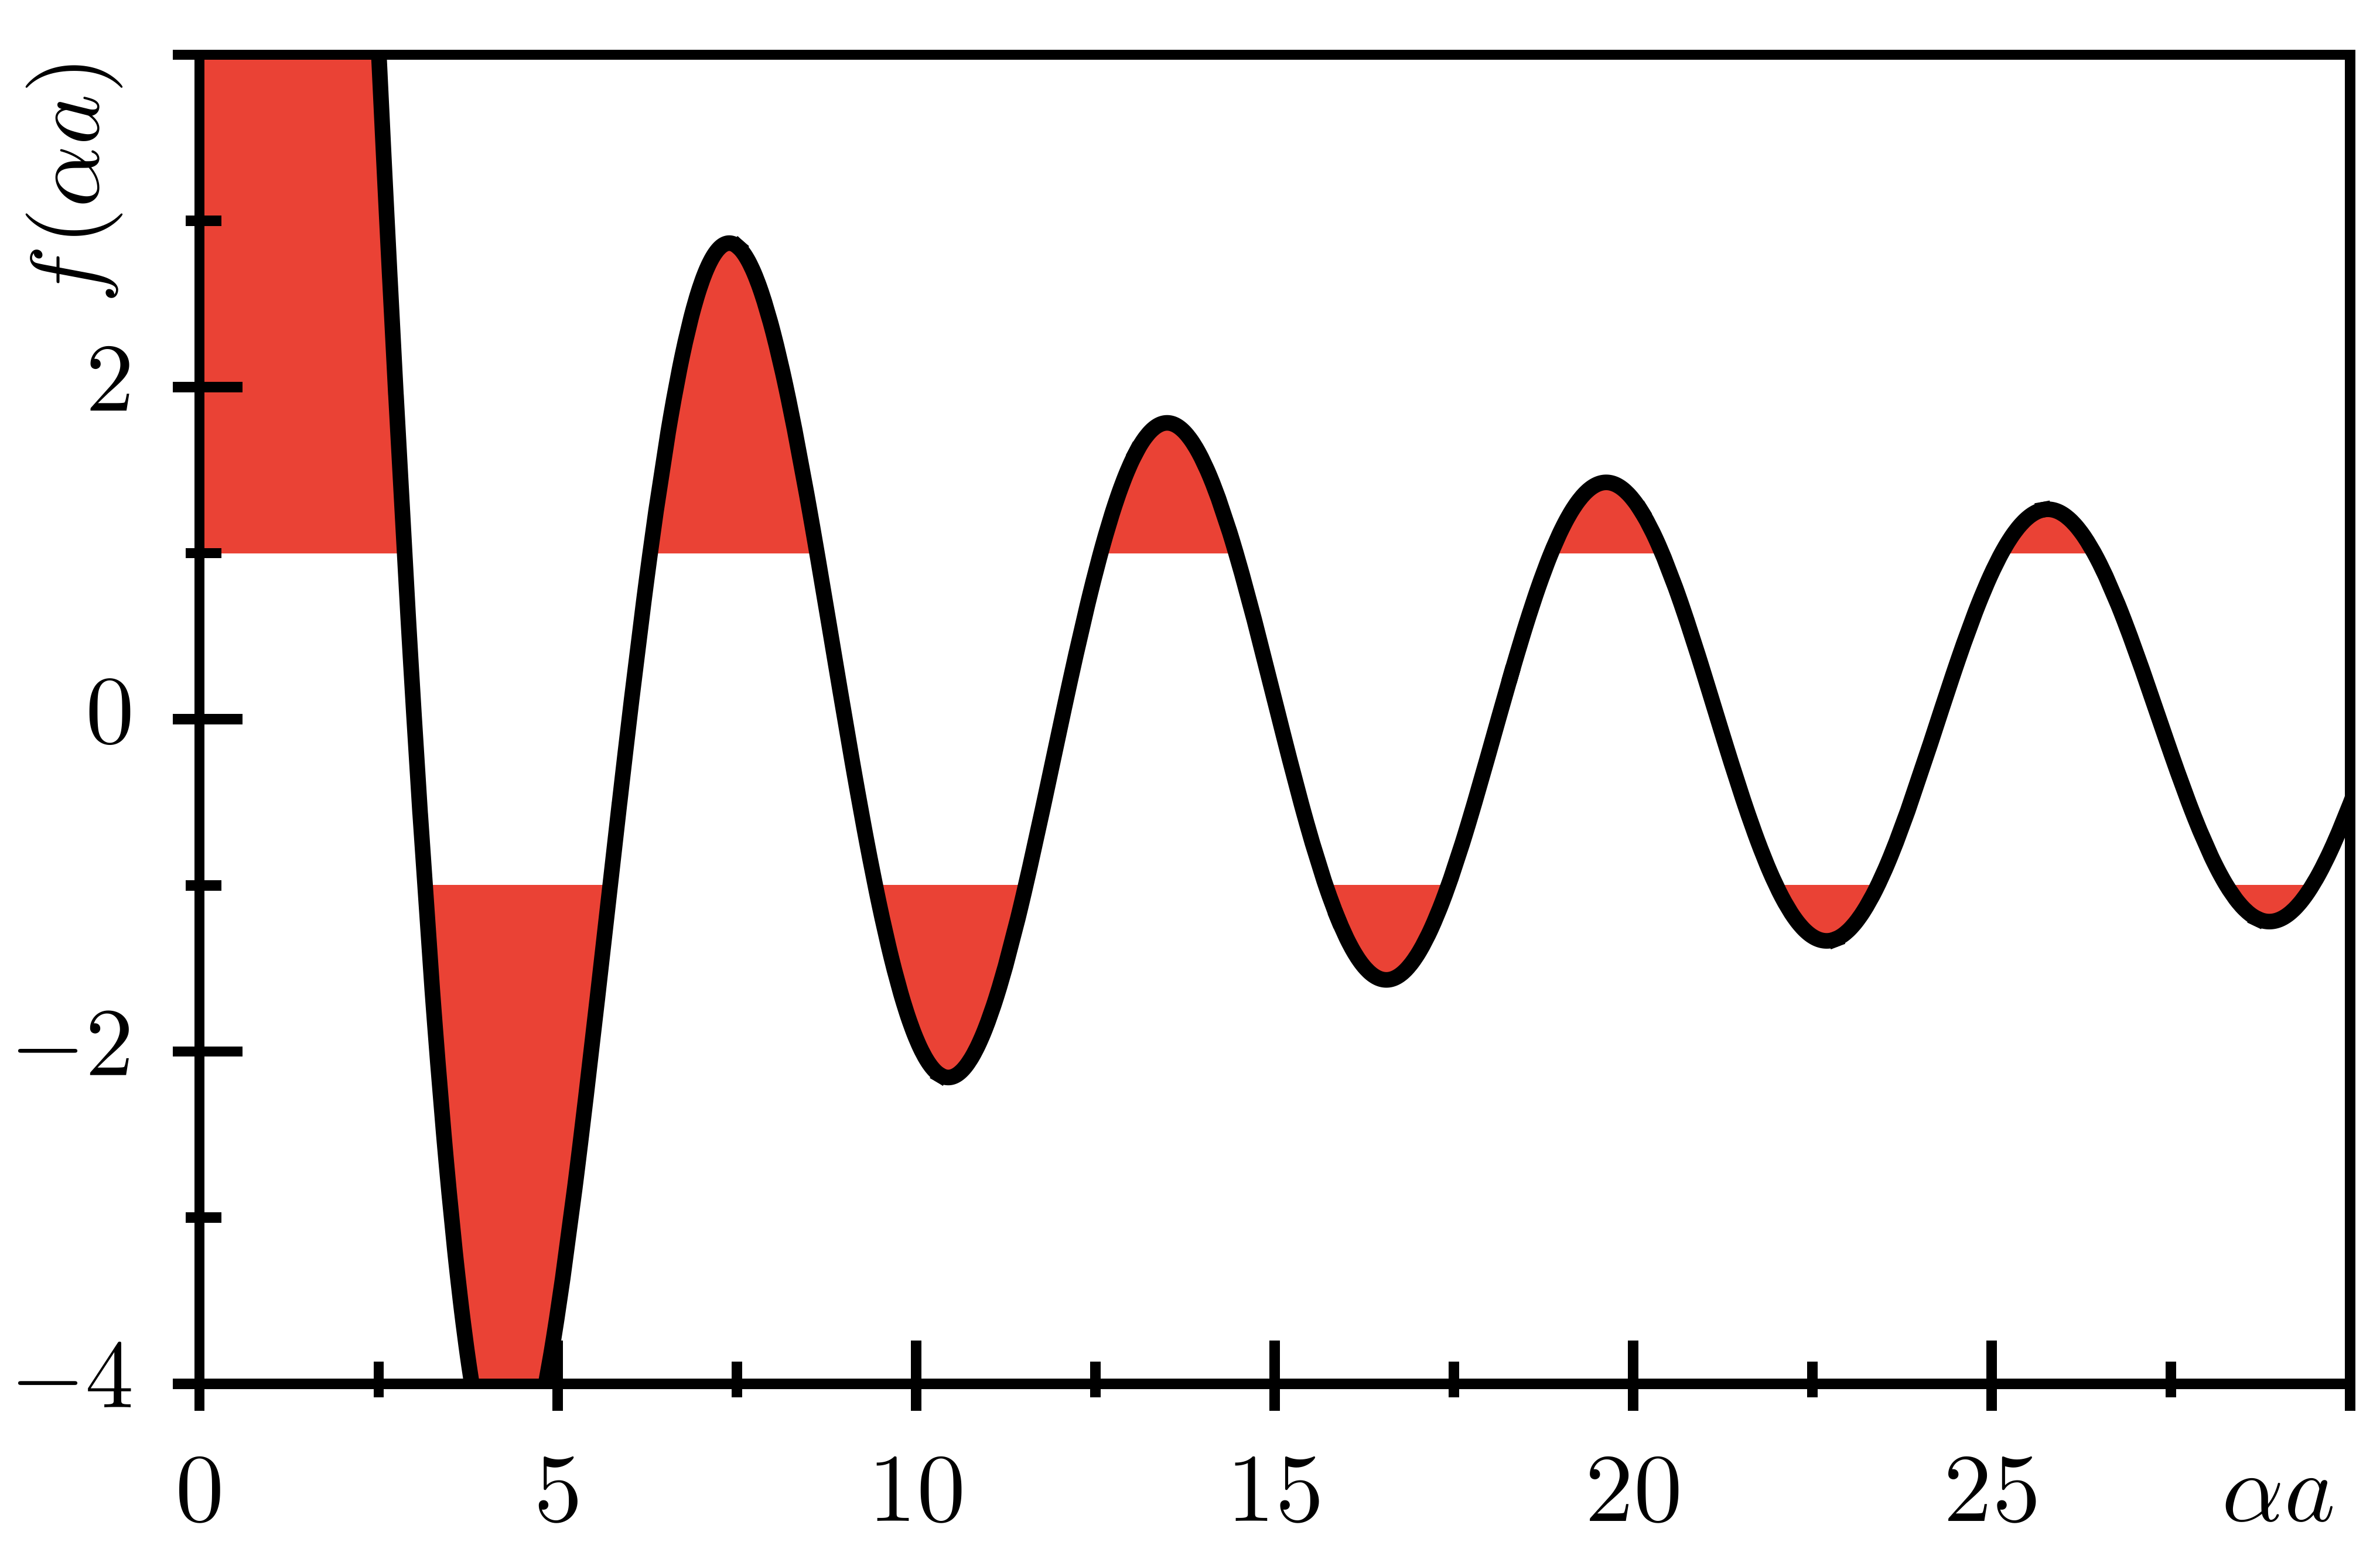
\includegraphics{figures/kronig_penney_transcendental.png}}
    \subfigure[]{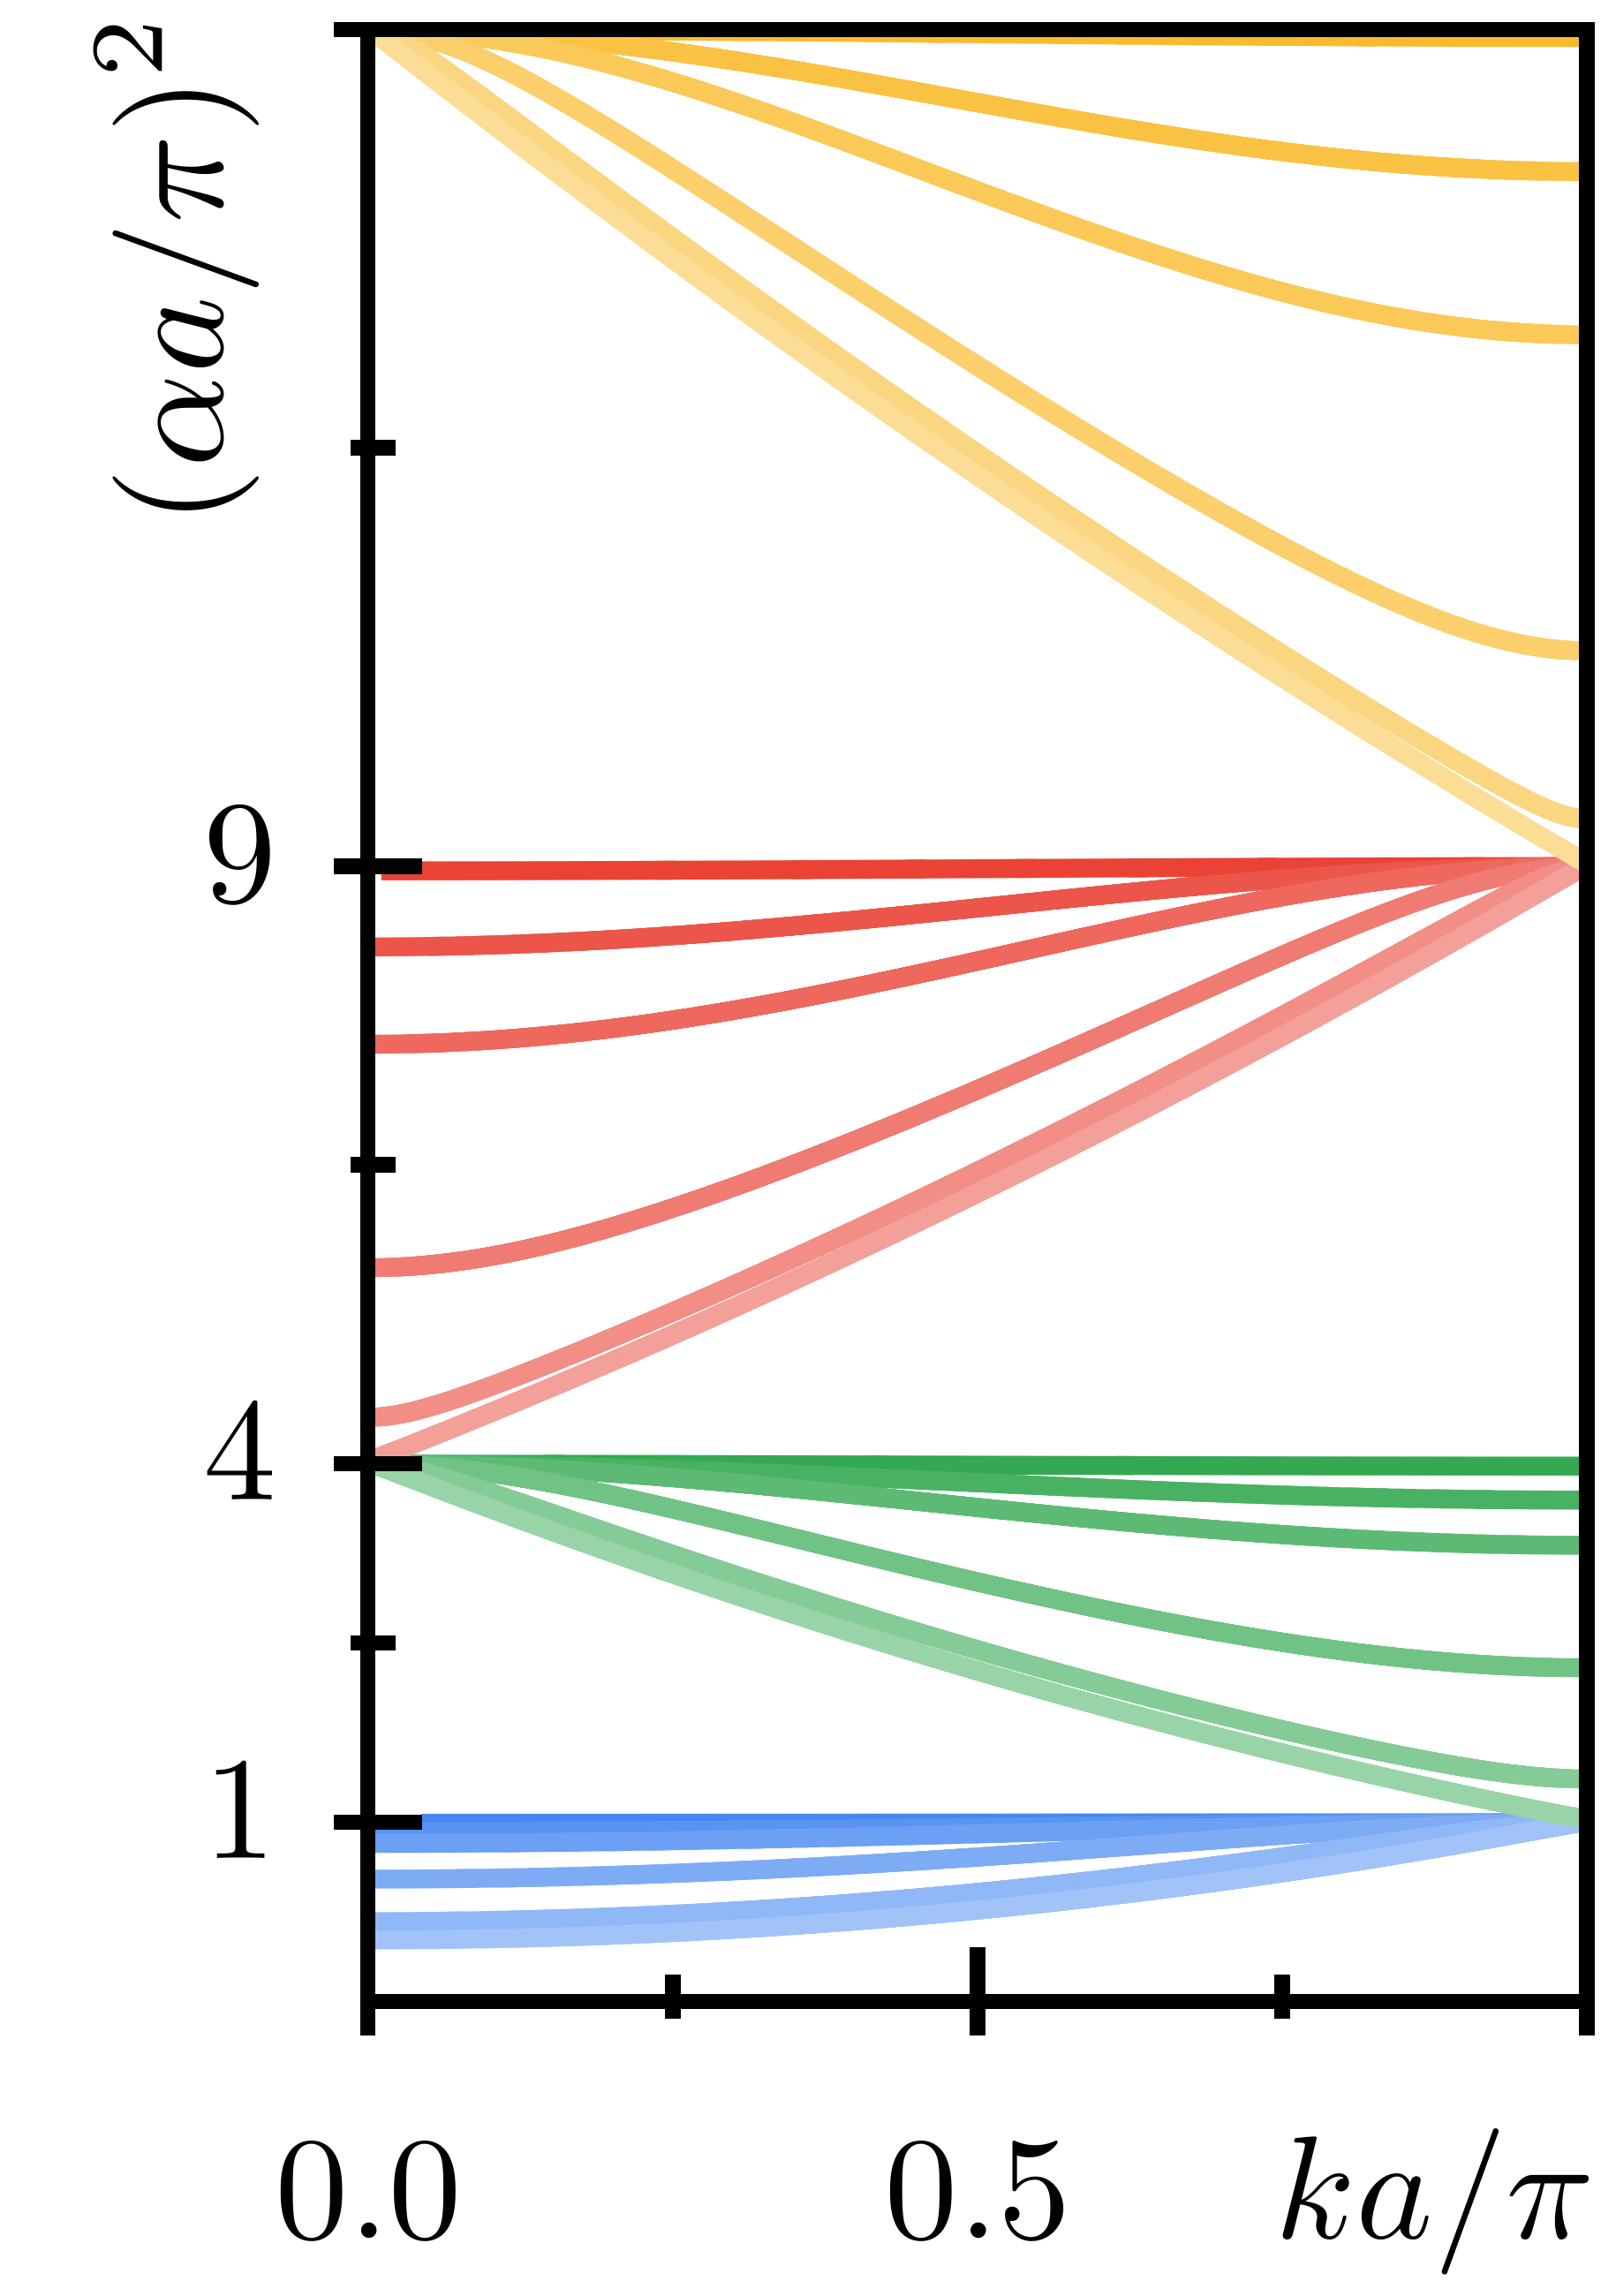
\includegraphics{figures/kronig_penney_dispersion_2.png}}
    \subfigure[]{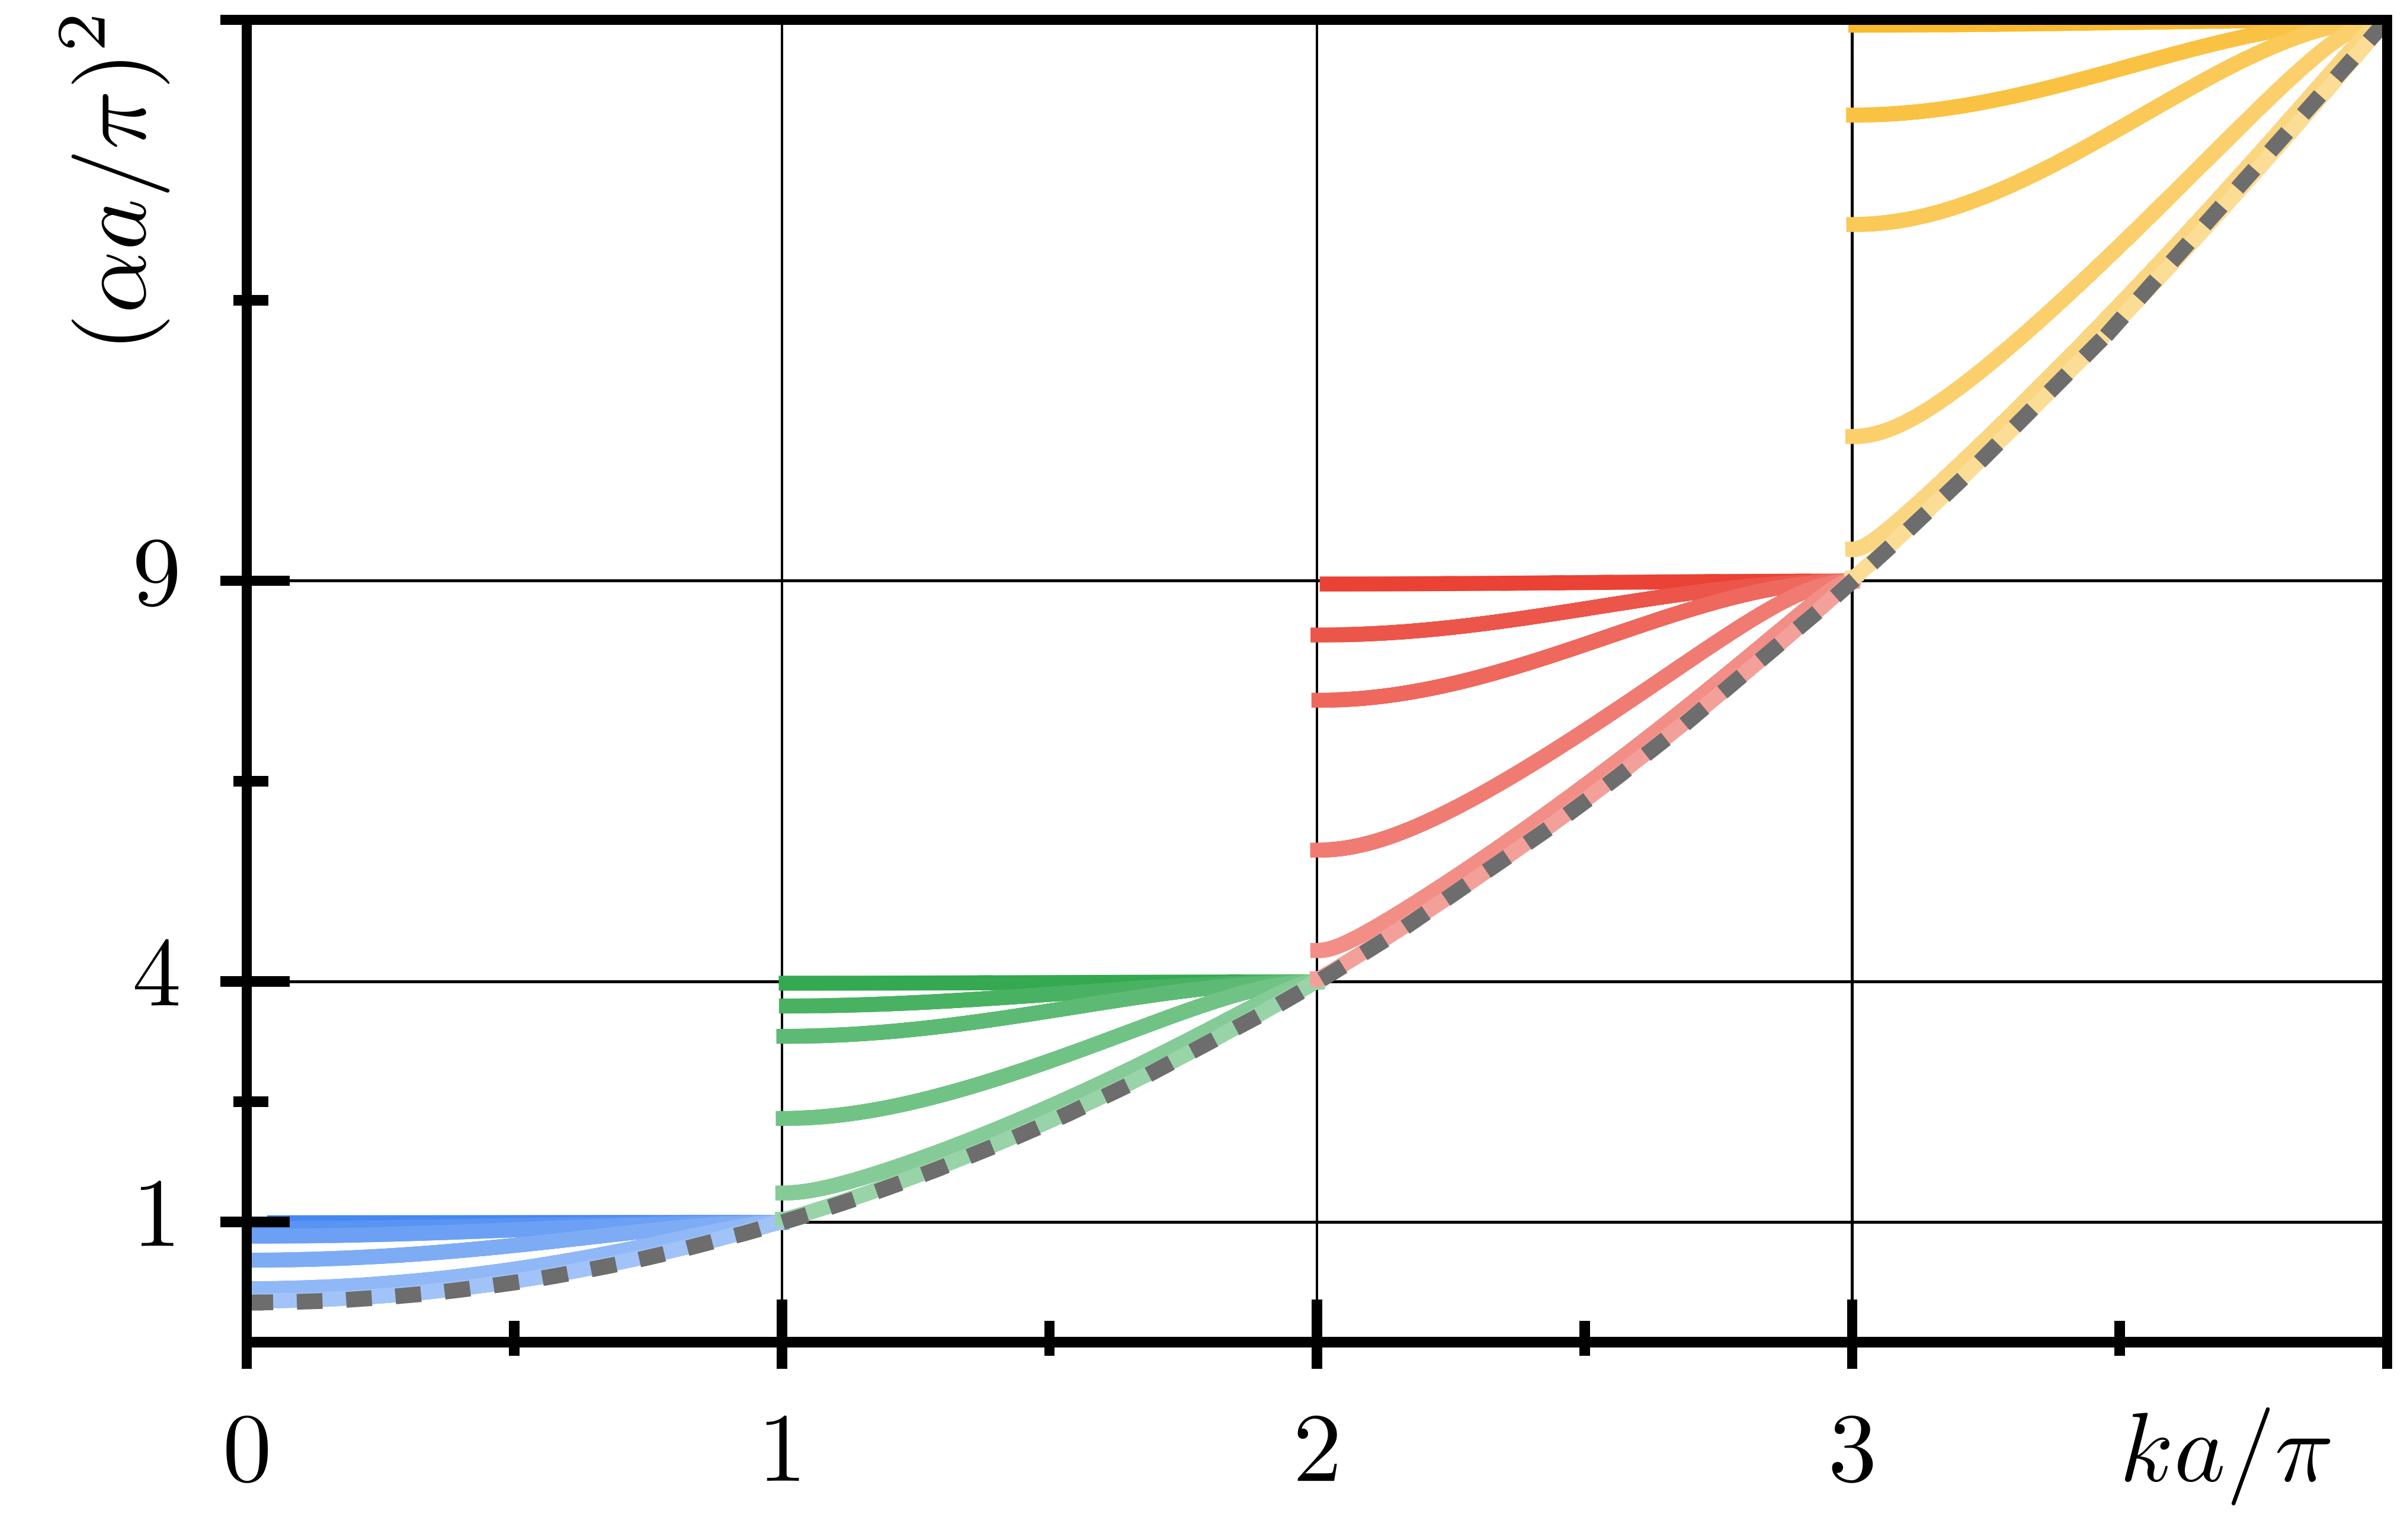
\includegraphics{figures/kronig_penney_dispersion_1.png}}
    \caption{
    (a) Plot of the right-hand-side of the transcendental equation. Solutions do not exist in the red regions.
    (b)-(c) Shapes of the dispersion relation $(\alpha a/\pi)^2$ versus crystal momentum $ka/\pi$ given by \cref{eq:kronig_penney_transcendental_equation_approx_bound}.
    Different opacity (transparent to colors) represent increasing values of $P\in\{0.1,1,5,20,50,1000\}$.
    (c) The properties of the wave functions allow to uniquely relate the crystal momentum $ka$ to an energy $\alpha a$ in which the limit of free electrons [i.e. $P\rightarrow0$] is pronounced.}
    \label{fig:kronig_penney_dispersion}
\end{figure}

If $P=0$, we are left with the energy-momentum relation of free electrons $k=\alpha$ and thus $E_0={\hbar^2k^2}/({2m})$.
If we approach $P\rightarrow\infty$, the allowed energies are formed by the roots of $\sin(\alpha a)$, i.e.
\begin{align}
    E_{\infty,n_b}=(\hbar n_b\pi)^2/(2ma^2),
    \label{eq:kronig_penney_energy_tb}
\end{align}
for which the level spacing is given by the squares of integer numbers ($n_b=1,2,\dots$).
The intermediate regimes $0<P<\infty$ can be solved by numerical evaluation of \cref{eq:kronig_penney_transcendental_equation_approx_bound} and are plotted in \cref{fig:kronig_penney_dispersion} (a).
Straightforward evaluation of $\arccos(f)$ yields the so-called ``reduced zone scheme'' displayed in \cref{fig:kronig_penney_dispersion} (b).

To get an analytic understanding of the wave functions in the above limit, let's focus on the region without potential (i) [remember that one is interested in the limit $b\rightarrow0$]
\begin{align}
    \psi_{\alpha k}^{\rm (i)}(x) = \re^{\ri kx}u_{\alpha k}^{\rm (i)}(x),
    \quad
    u_{\alpha k}^{\rm (i)}(x) = A\re^{\ri(\alpha-k) x} + A'\re^{-\ri(\alpha+k) x},
    \quad
    u_{\alpha k}^{\rm (i)}(x+na)=u_{\alpha k}^{\rm (i)}(x)
    \label{eq:kronig_penney_wavefunctions}
\end{align}
in which the prefactors are related by\footnote{An additional constraint for $AA^*$ is found by requiring normalization of the wave functions, which allows to compute expectation values. However, it is not needed for the purpose of this section and I refer to \cite{KronigPenney1931}.}
\begin{align}
    A' = -A\frac{1-\re^{\ri(\alpha-k)a}}{1-\re^{-\ri(\alpha+k)a}}.
    \label{eq:kronig_penney_constants}
\end{align}

Starting from \cref{eq:kronig_penney_transcendental_equation_approx_bound}, we see that for any solution $\alpha a$ satisfying $f(\alpha a)=\cos(k a)$ there is an infinite number of symmetric points in momentum space which fulfill the same equation, i.e. (a) $ka + 2n\pi$ and (b) $-ka+2n\pi$.
Close inspection of \cref{eq:kronig_penney_wavefunctions,eq:kronig_penney_constants} reveals that a transformation according to (a) leaves the wave function invariant, while (b) maps it to the solutions of $-ka$, $-\alpha a$.

In other words, (a) is merely a shift by a unit reciprocal vector and (b) flips the direction of the propagating wave, hence establishes a mirror symmetry at the $ka=0$ axis.
The properties (a) and (b) allow to define the ``unfolding'' of the reduced zone scheme:
without loss of generality, a crystal momentum $n_b\pi\leq ka<(n_b+1)\pi$ can be uniquely connected to an energy value $n_b\pi\leq \alpha a<(n_b+1)\pi$ by introducing a band index $(n_b=0,1,\dots)$.
Here, the limit of free particles ($P=0$) is readily restored, since \cref{eq:kronig_penney_constants} vanishes for $\alpha a = ka$ (except for the special points $ka=n_b\pi$).

At the special points $ka=n_b\pi$, \cref{eq:kronig_penney_constants} is actually ill defined and evaluates to the two viable solutions $A'=\pm A$, which can be understood from the two non-commuting limits
\begin{align}
    -\lim_{\alpha a \searrow n_b\pi}\frac{1-\re^{\ri(\alpha a-n_b\pi))}}{1-\re^{-\ri(\alpha a+n_b\pi)}}
    =
    -\lim_{\epsilon\searrow0}\frac{1-\re^{+\ri\epsilon}}{1-\re^{-\ri\epsilon}}
    =
    \lim_{\epsilon\searrow0}\re^{+\ri\epsilon}\frac{1-\re^{-\ri\epsilon}}{1-\re^{-\ri\epsilon}}
    =
    +1,
    \\
    -\lim_{k a \searrow n_b\pi}\frac{1-\re^{\ri(n_b\pi - ka))}}{1-\re^{-\ri(n_b\pi+ka)}}
    =
    -\lim_{k a \searrow n_b\pi}\frac{1-\re^{-\ri(n_b\pi + ka))}}{1-\re^{-\ri(n_b\pi+ka)}}
    =
    -1.
\end{align}
The two allowed eigenfunctions are standing waves $\propto \cos(kx),\sin(kx)$.
By reformulating the special points in terms of the particles' de Broglie wavelength $\lambda=2\pi/k$, the formation of standing waves can be understood as a residual effect of (constructive) Bragg reflection on a periodic grid structure.
Standing waves are obtained if the particle's de Broglie wavelength and the spacing of the potential satisfy $2a=n_b\lambda$.

In the limit $P\rightarrow\infty$, the energy $E_{\infty,n_b}$ assumes the discrete values in \cref{eq:kronig_penney_energy_tb} resulting in motionless eigenstates -- the resulting waves are tightly bound to the potential minimum.
If we relax this limit a bit, i.e. $P\gg 1$, a reasonable approximation of the lowest band curvature is obtained by a first order Taylor series of \cref{eq:kronig_penney_transcendental_equation_approx_bound} resulting in the typical dispersion relation for tight binding systems, i.e.
\begin{align}
    E_{P\gg1,1}\approx t_0 + t_1 \cos(k a),
    \quad
    t_0 = + E_{\infty,1} - \frac{\pi^2 \hbar^4}{a^3 m^2 b V_0},
    \quad
    t_1 = -\frac{\pi^2\hbar^4}{a^3 m^2 bV_0}.
    \label{eq:kronig_penney_tight_binding_dispersion}
\end{align}
This concludes the pedagogic recap of the Kronig-Penney model, and I proceed by giving a more generic recipe to solve arbitrary periodic potentials.

In order to tackle generic potentials, let us expand the Schrödinger equation in reciprocal space through the following identities\footnote{The reciprocal space provides a way to Fourier-transform as the functions $\re^{\ri {\bm G r}}$ form a basis on the primitive cell of the real lattice over the square-integrable functions. In particular, the functions satisfy the orthogonality equation $\delta_{\bm G, \bm G'}=\frac1{V}\int\rd^dr\,\re^{\ri({\bm G-\bm G'}){\bm r}}$.}
\begin{align}
    V_{ae}({\bm r}) = \sum_{\bm G}V_{ae}{}_{\bm G}\re^{\ri {\bm G r}},
    \quad
    V_{ae}{}_{\bm G} = \frac1{V}\int\rd^dr\,V_{ae}({\bm r})\re^{-\ri {\bm G r}},
    \\
    u_{n{\bm k}}({\bm r}) = \sum_{\bm G}u_{n{\bm k}}{}_{\bm G}\re^{\ri {\bm G r}},
    \quad
    u_{n{\bm k}}{}_{\bm G} = \frac1{V}\int\rd^dr\,u_{n{\bm k}}({\bm r})\re^{-\ri {\bm G r}},
\end{align}
in which $V$ is the volume of the primitive unit cell.
Straightforward evaluation yields the algebraic eigenvalue problem for the unknown functions $u_{n{\bm k}}{}_{\bm G}$
\begin{align}
    \frac{\hbar^2}{2m}({\bm G}+{\bm k})^2u_{n{\bm k}}{}_{\bm G}+\sum_{\bm G'}V_{ae}{}_{\bm G-\bm G'}u_{n{\bm k}}{}_{\bm G'} = E_{n{\bm k}}.
    \label{eq:periodic_lattices_numerics}
\end{align}
The dimension of the linear equation is infinite due to the sum over all reciprocal lattice vectors and has to be truncated if one wants to solve the equation numerically (the convergence of such a truncation has to be carefully checked).
Clearly, strongly confined potentials such as delta functions studied in the Kronig-Penney model are particularly bad candidates to solve numerically through evaluation of \cref{eq:periodic_lattices_numerics} because the resulting matrix equation will not be sparse and any truncation will result in a significant error.
%
%
%%%%%%%%%%%%%%%%%%%%%%%%%%%%%%%%%%
\section{Tight binding systems}
\label{sec:tight_binding_systems}
%%%%%%%%%%%%%%%%%%%%%%%%%%%%%%%%%%
%
%
The systems considered here are those of tightly bound constituents to the lattice centers.
Such types can be found in traditional solid state scenarios where the nuclei are well separated beyond the typical Bohr radius of the valence electrons, in setups of ultracold atoms trapped in optical lattices~\cite{Bloch2008}, in photonic waveguides~\cite{Lu2014} or polaritons~\cite{Amo2016}.
In all our works, we cover theoretical aspects of interacting tight binding models which can be experimentally realized in a variety of different setups.
For this reason, it will be useful to review briefly how these models are motivated from first principles, and how they can be understood in second quantization.

\begin{figure}
    \centering
    \subfigure[]{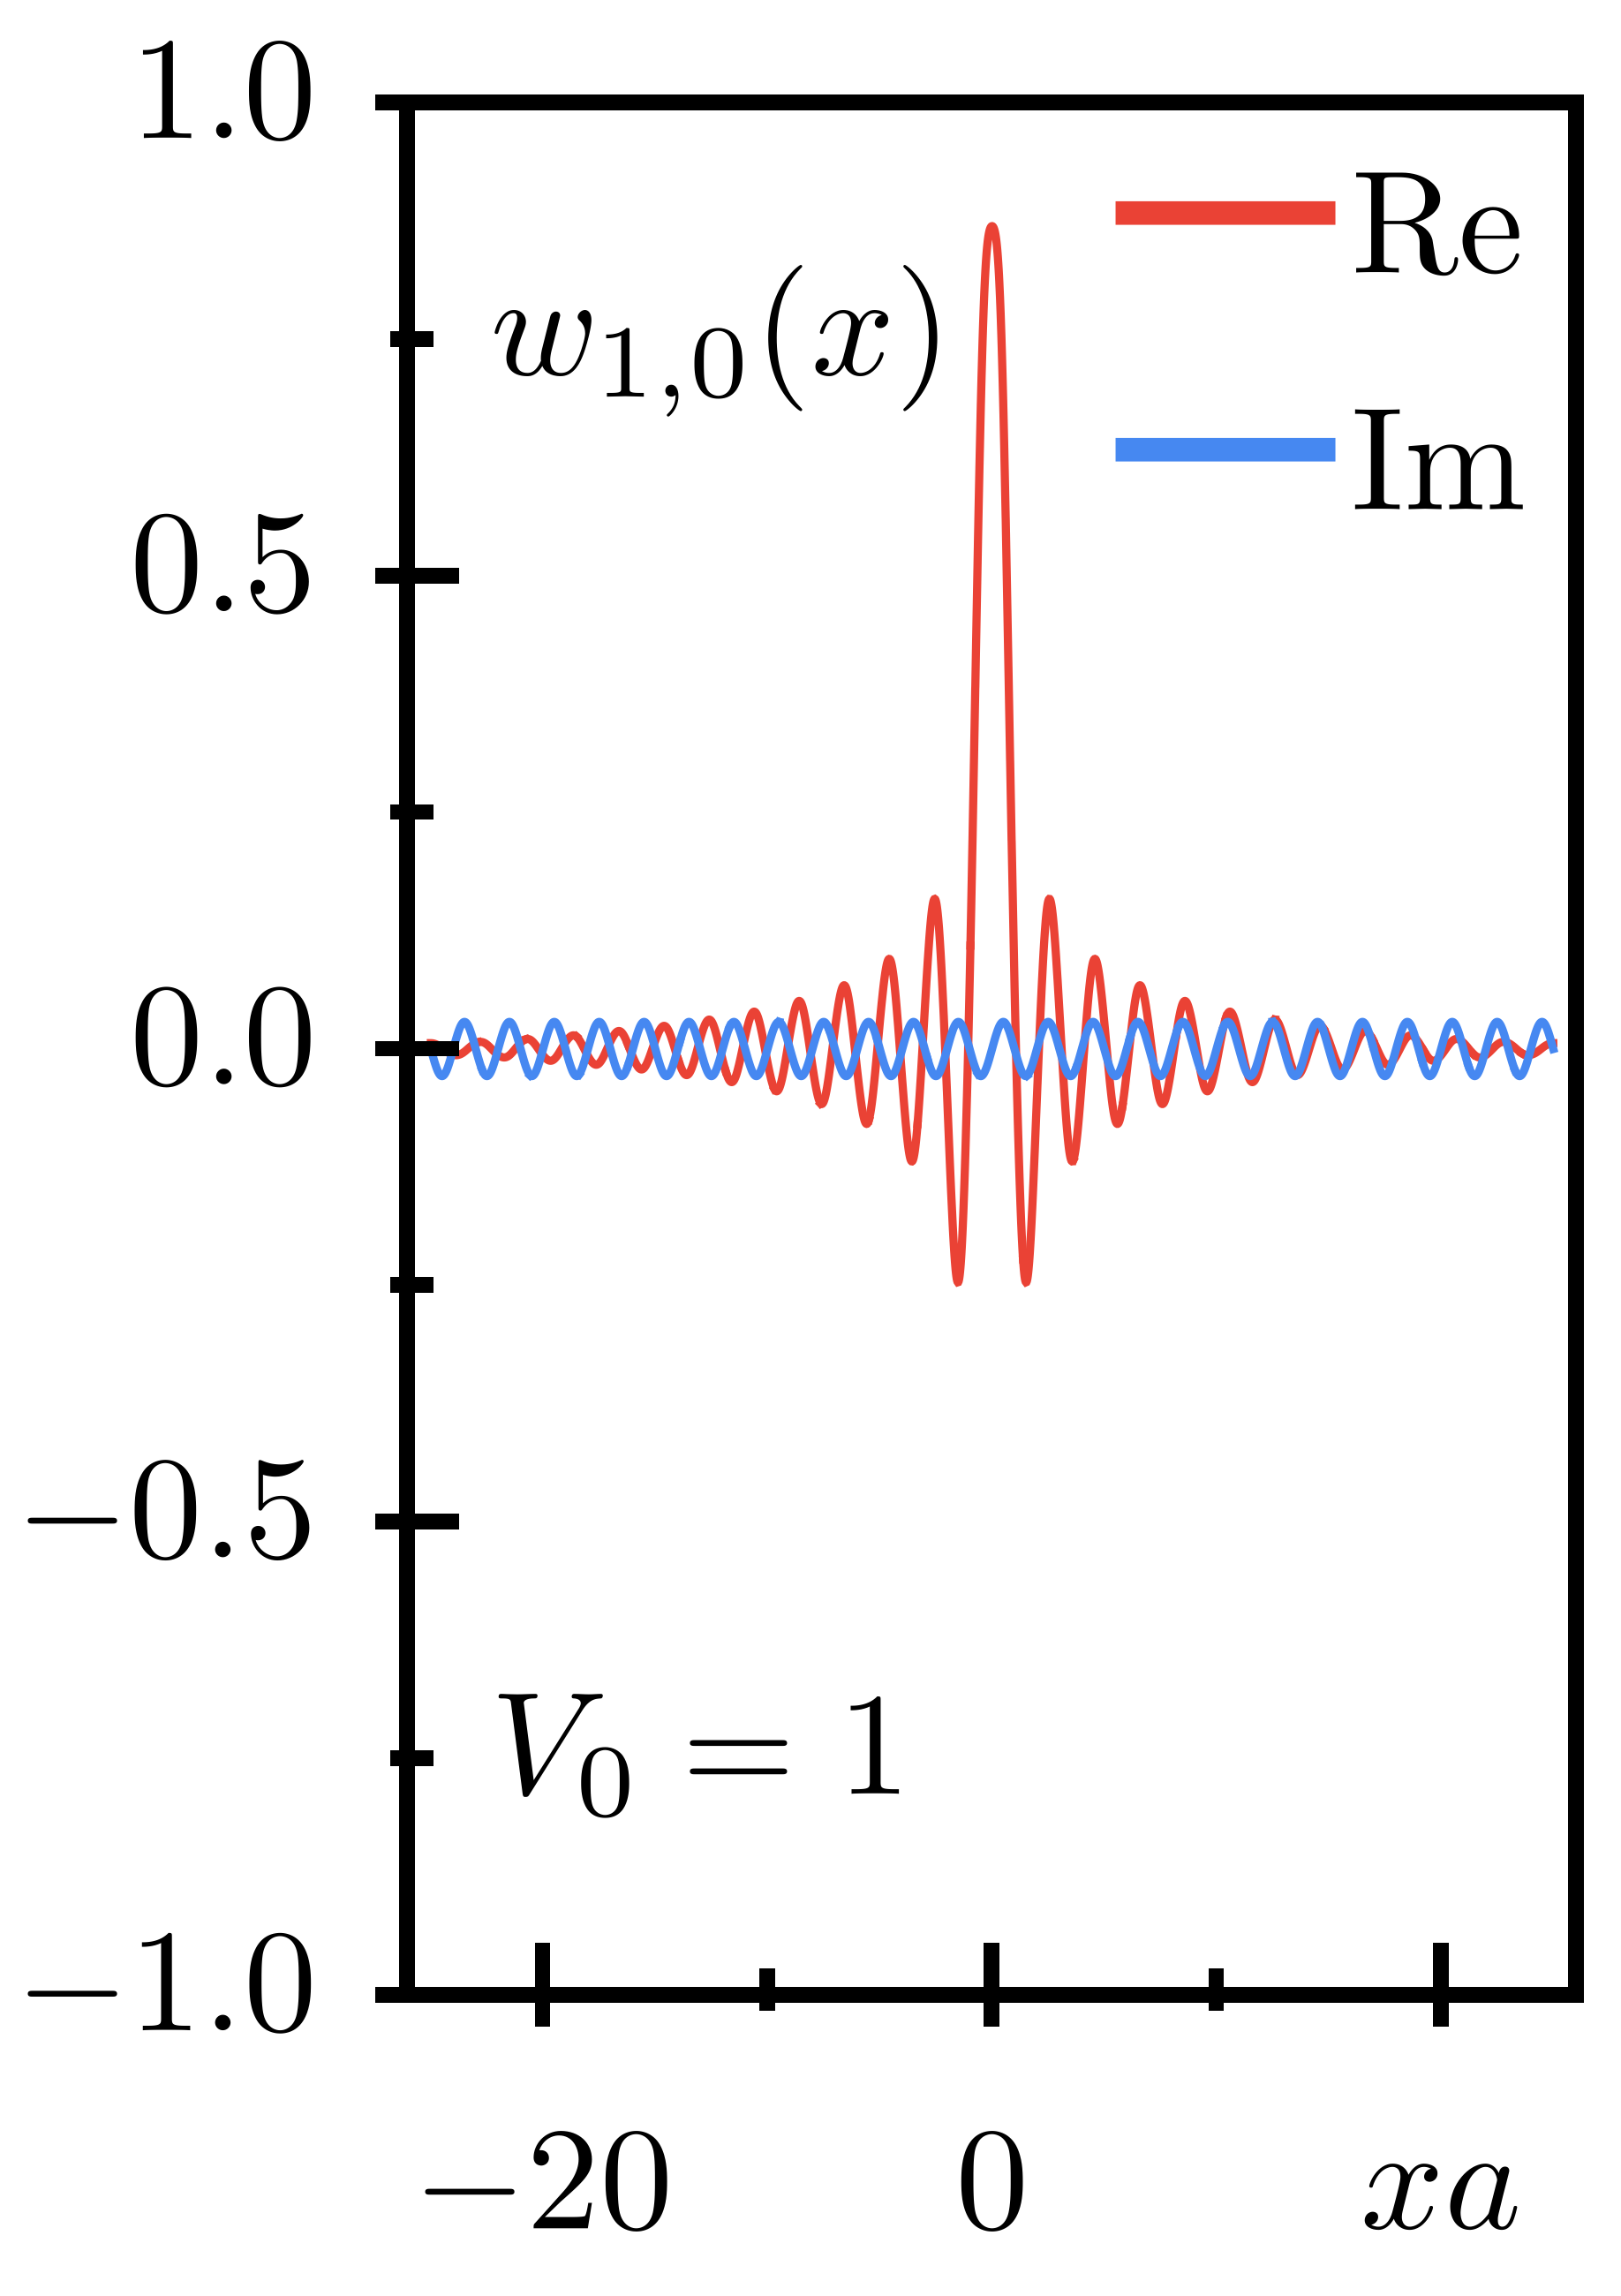
\includegraphics{figures/wannier1_1.png}}
    \subfigure[]{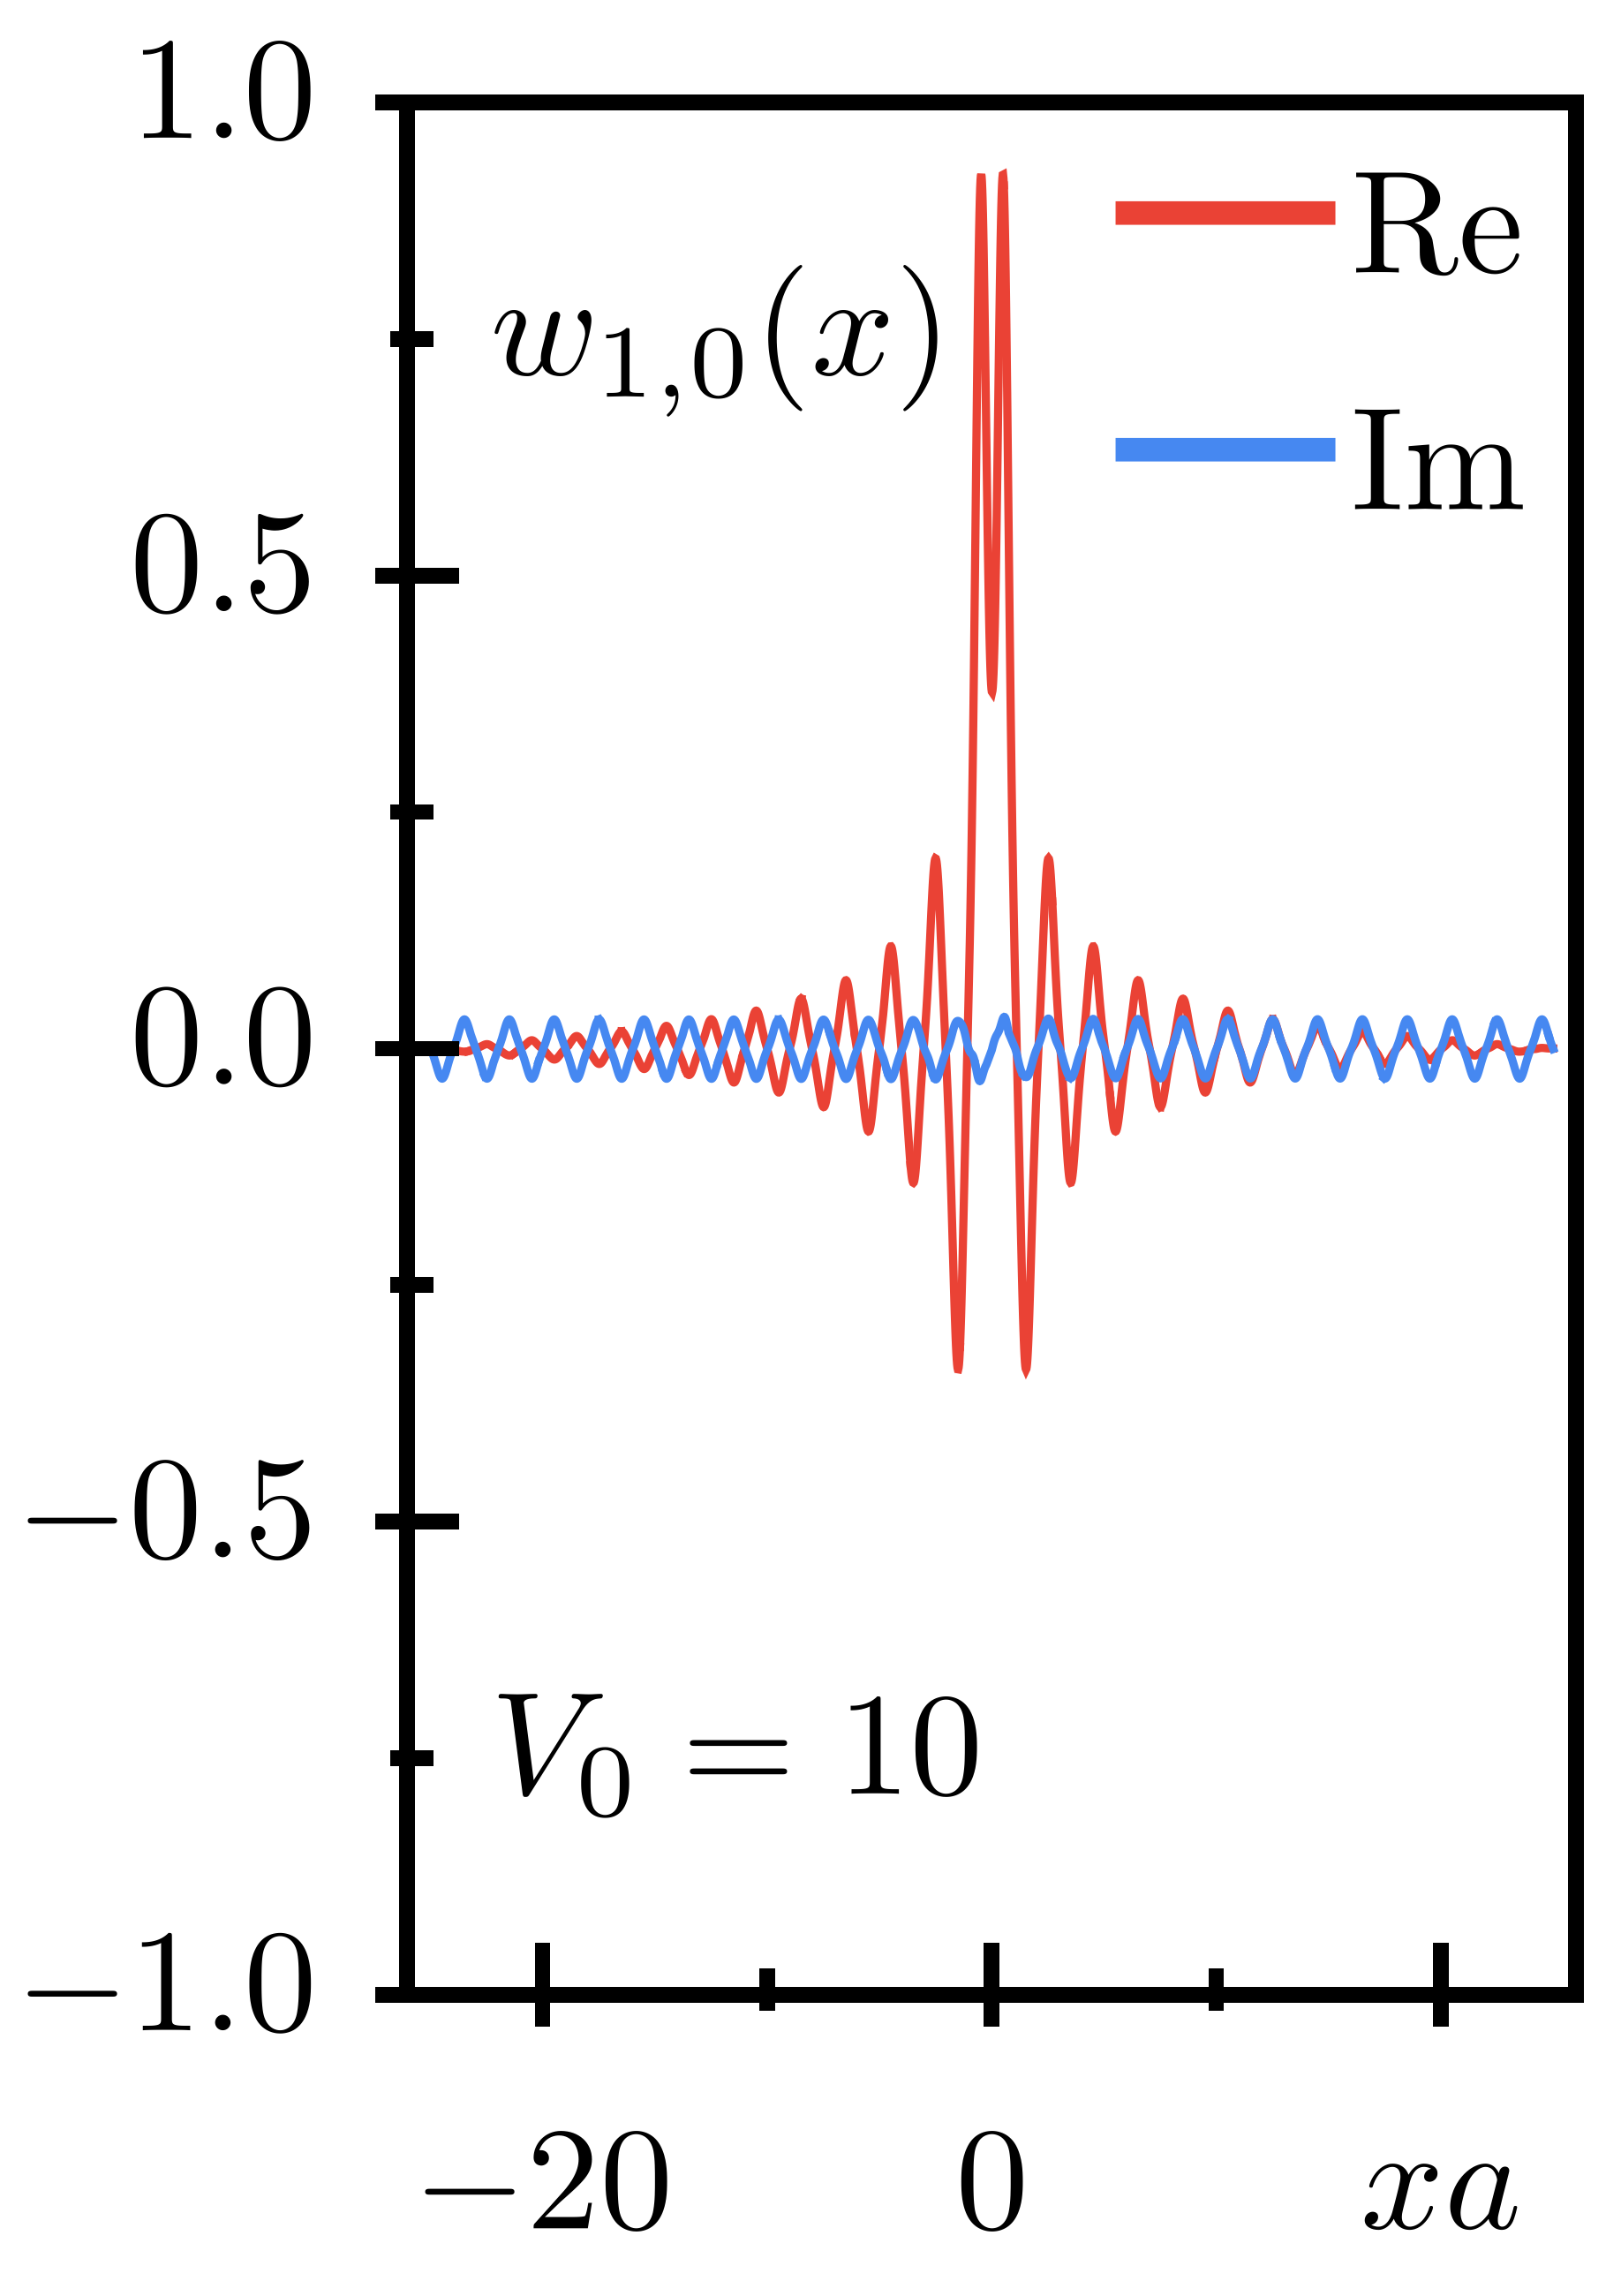
\includegraphics{figures/wannier1_10.png}}
    \subfigure[]{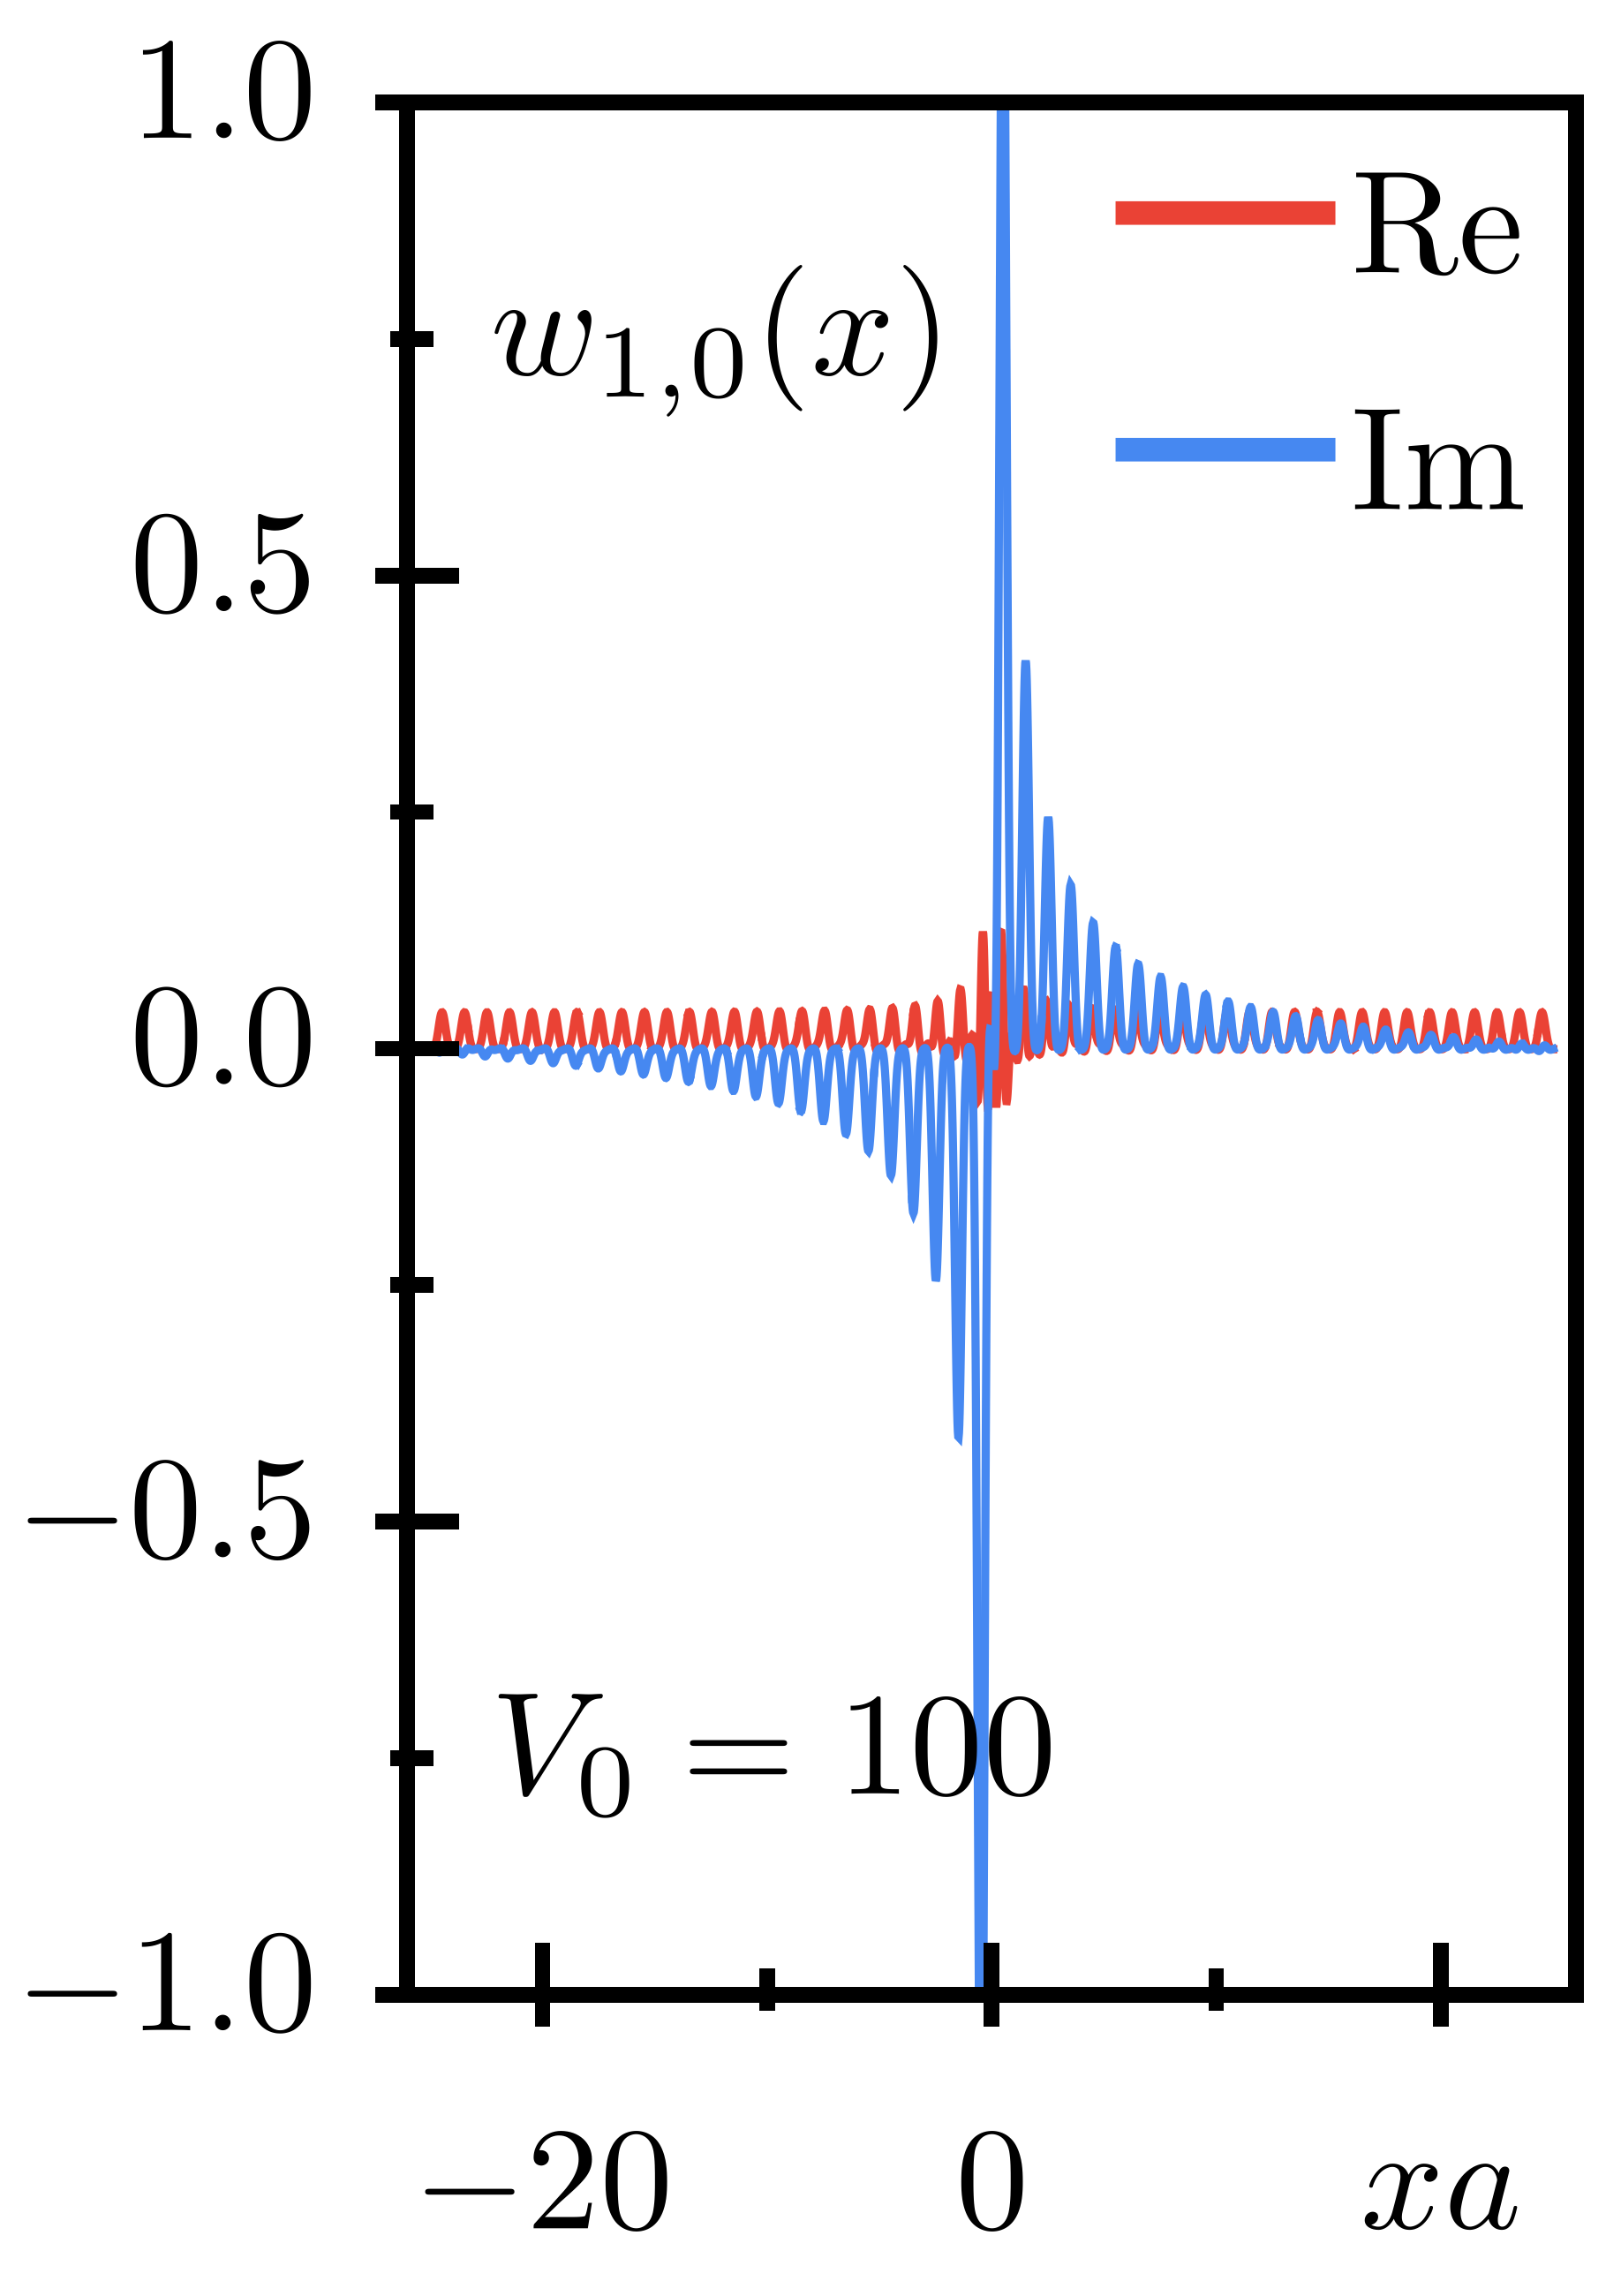
\includegraphics{figures/wannier1_100.png}}\\
    \subfigure[]{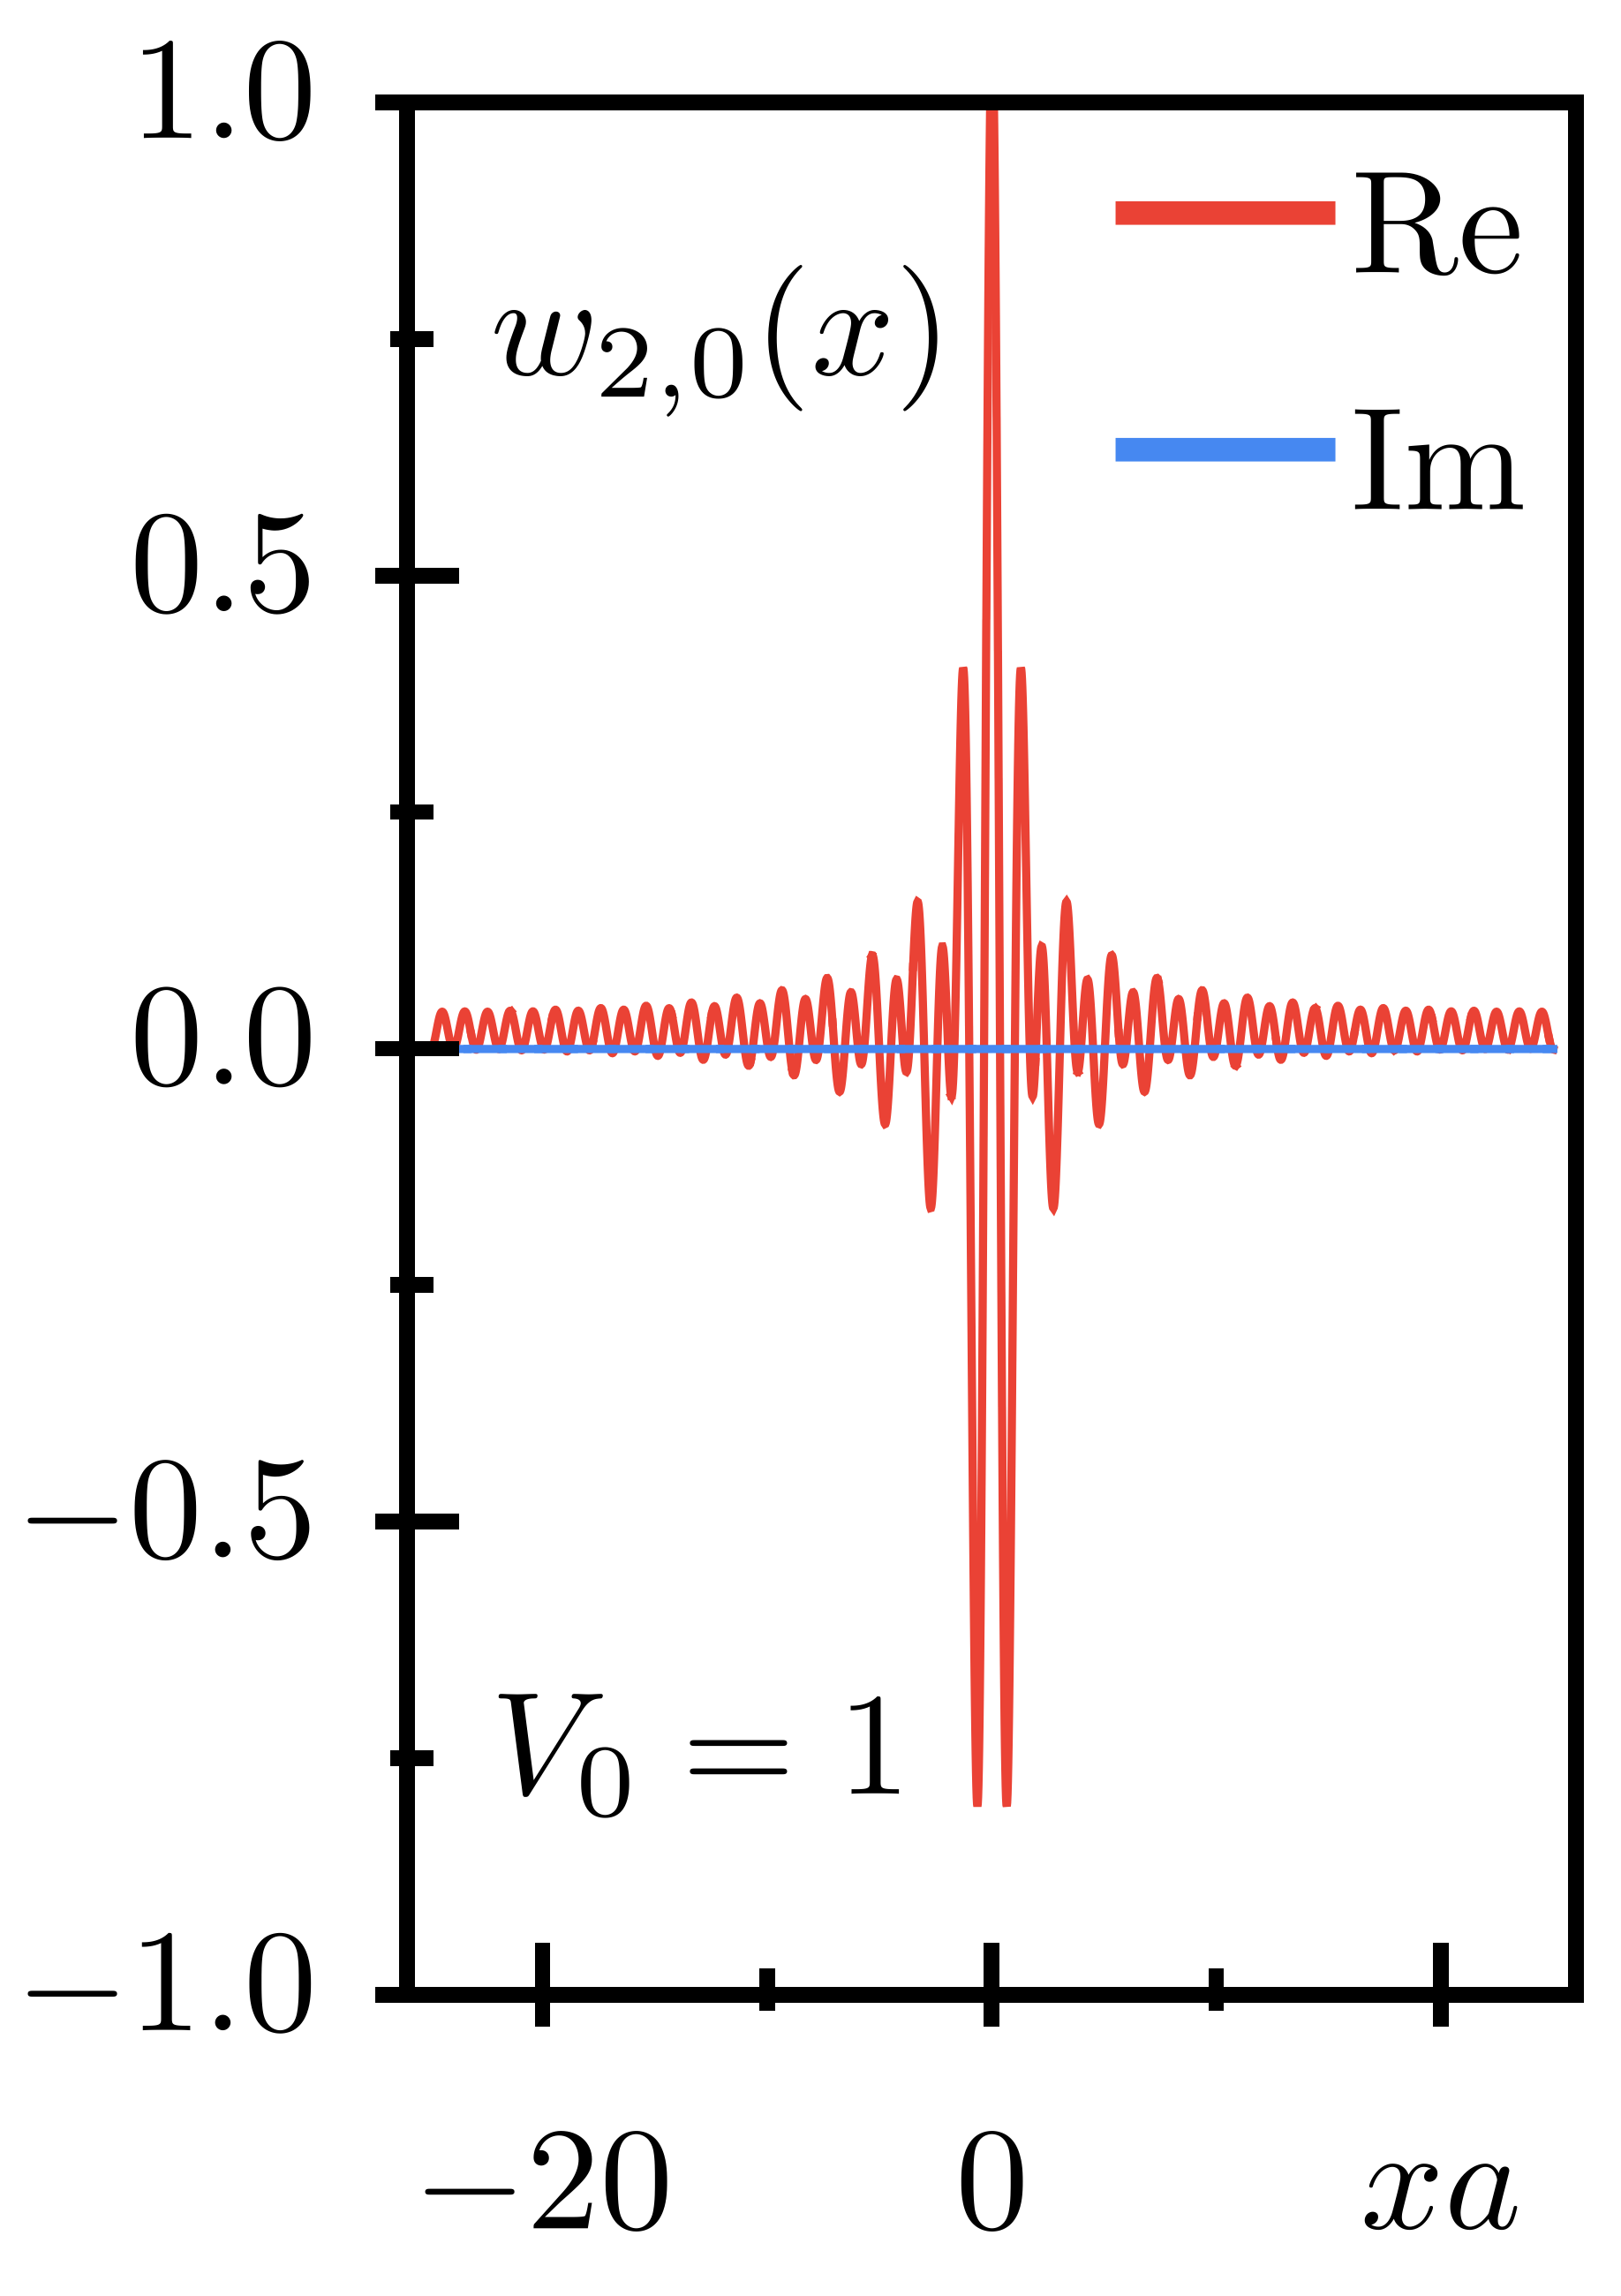
\includegraphics{figures/wannier2_1.png}}
    \subfigure[]{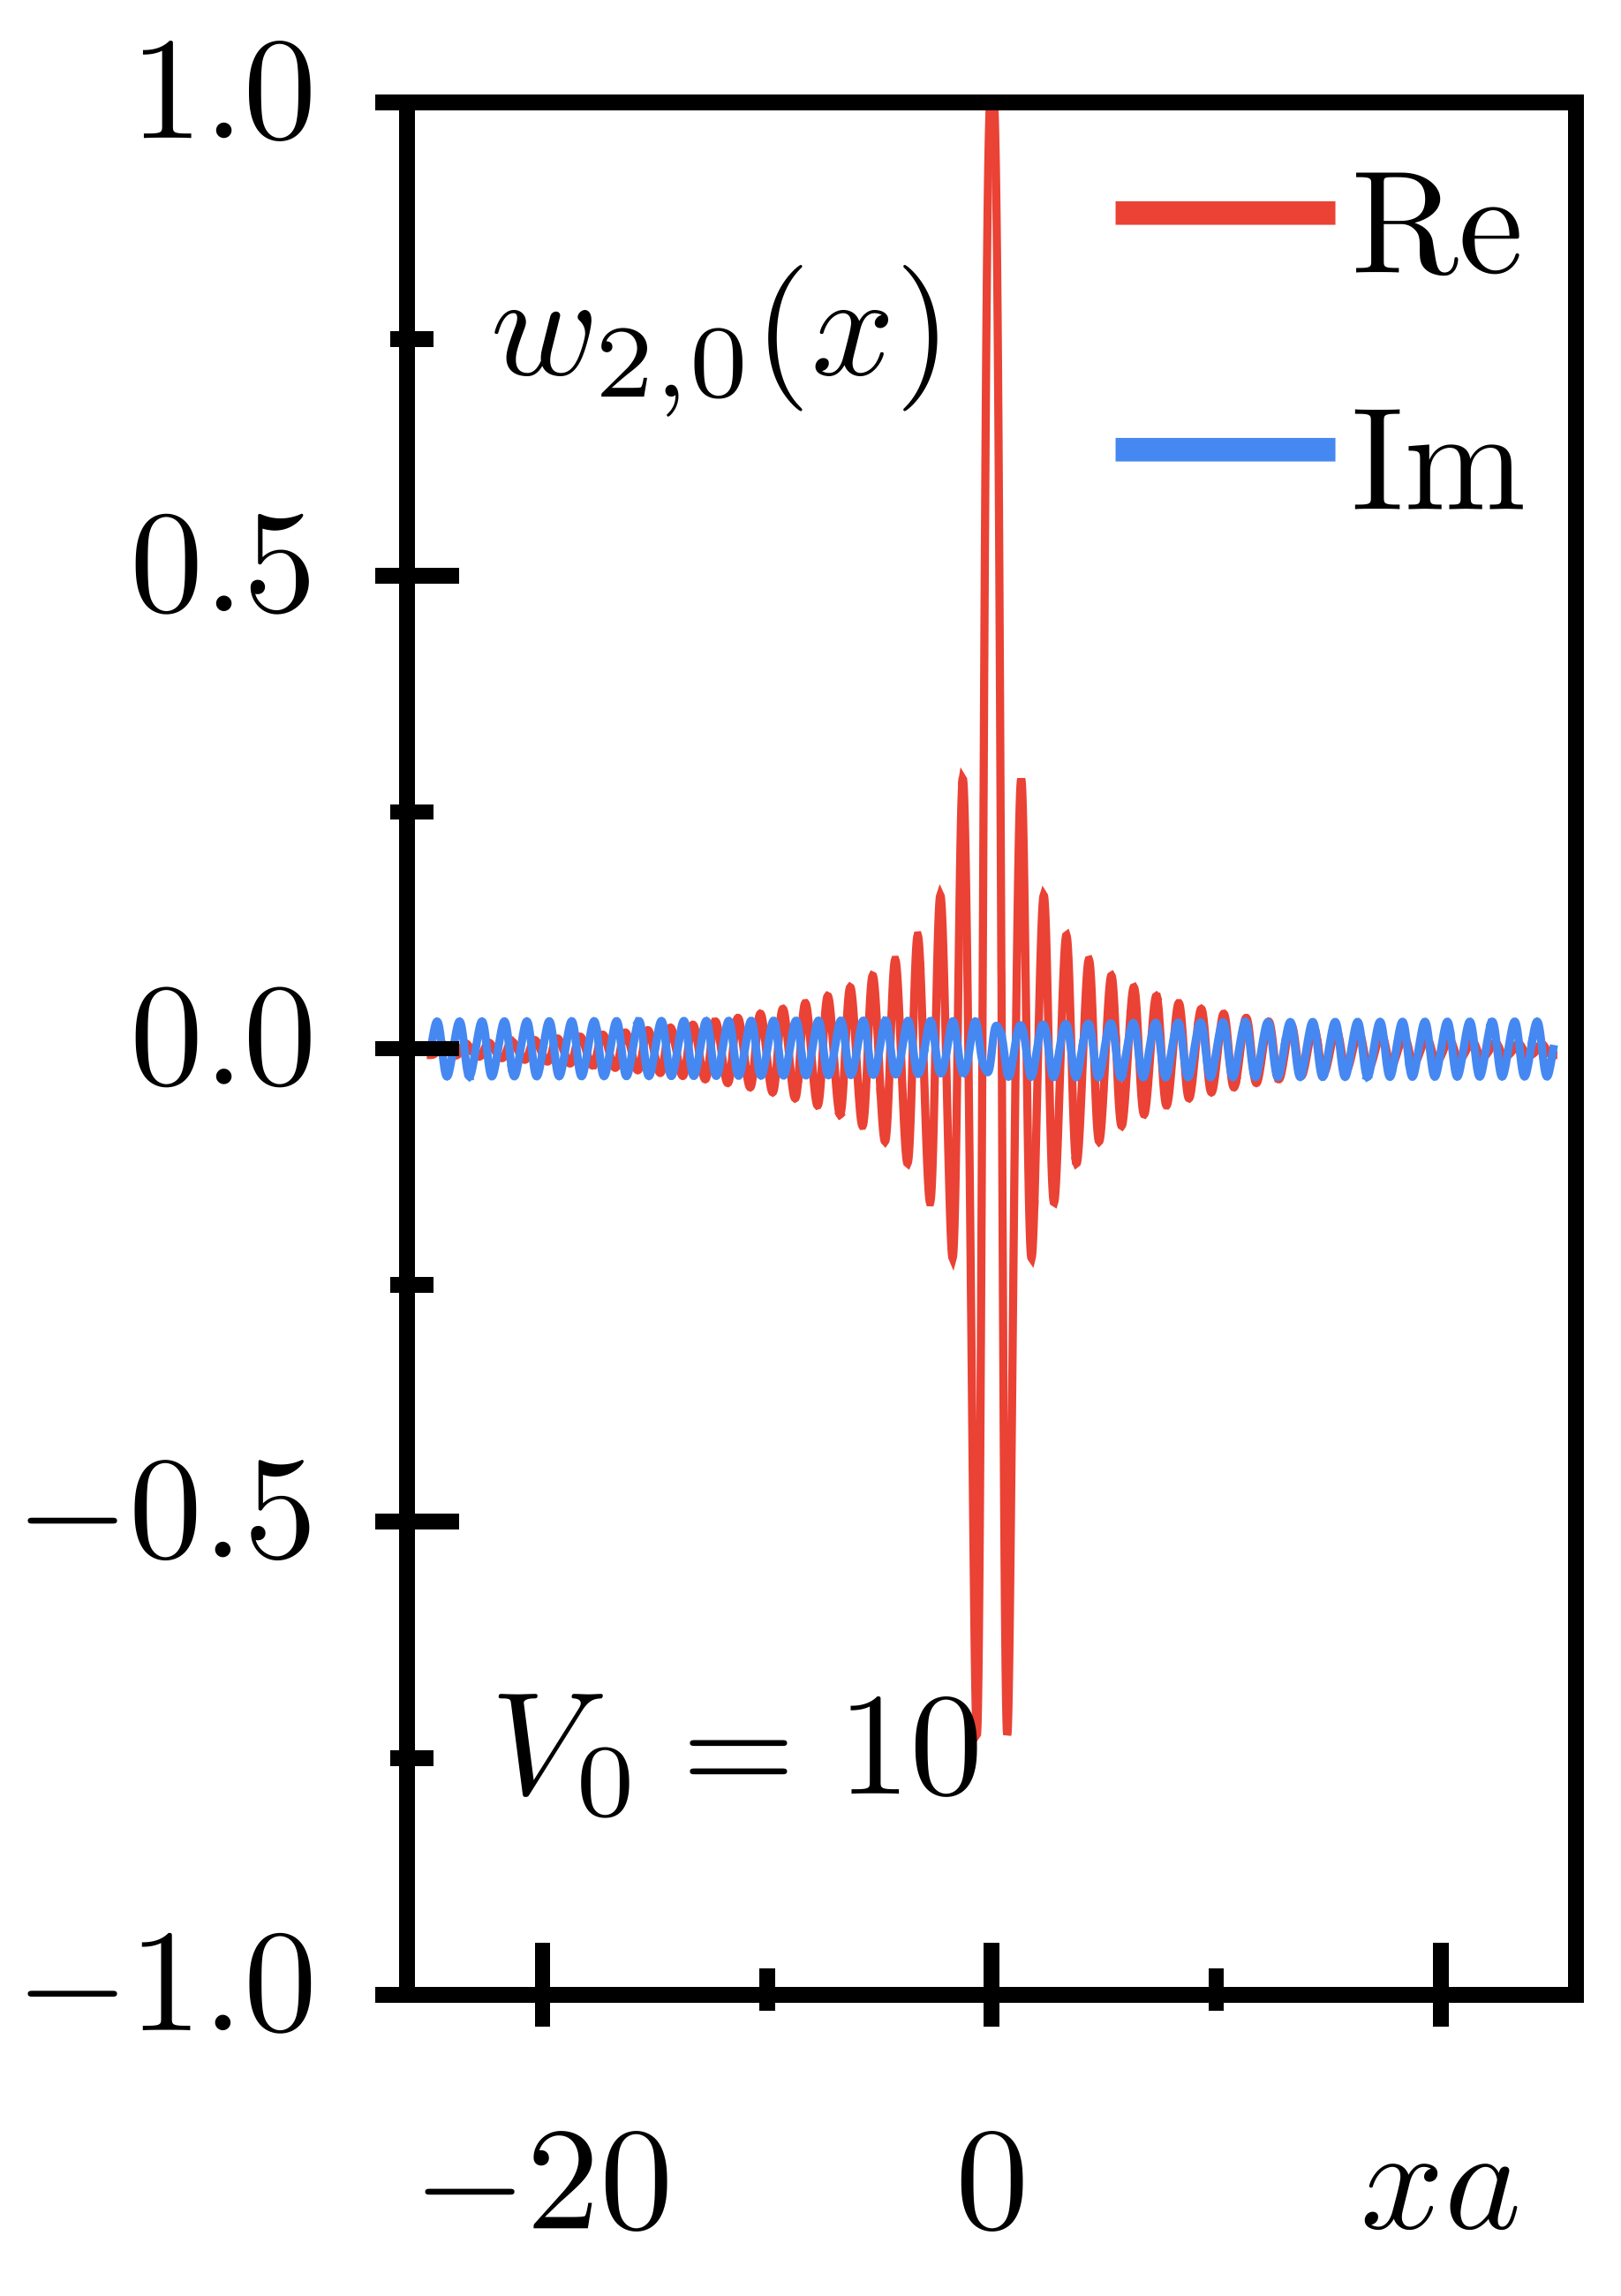
\includegraphics{figures/wannier2_10.png}}
    \subfigure[]{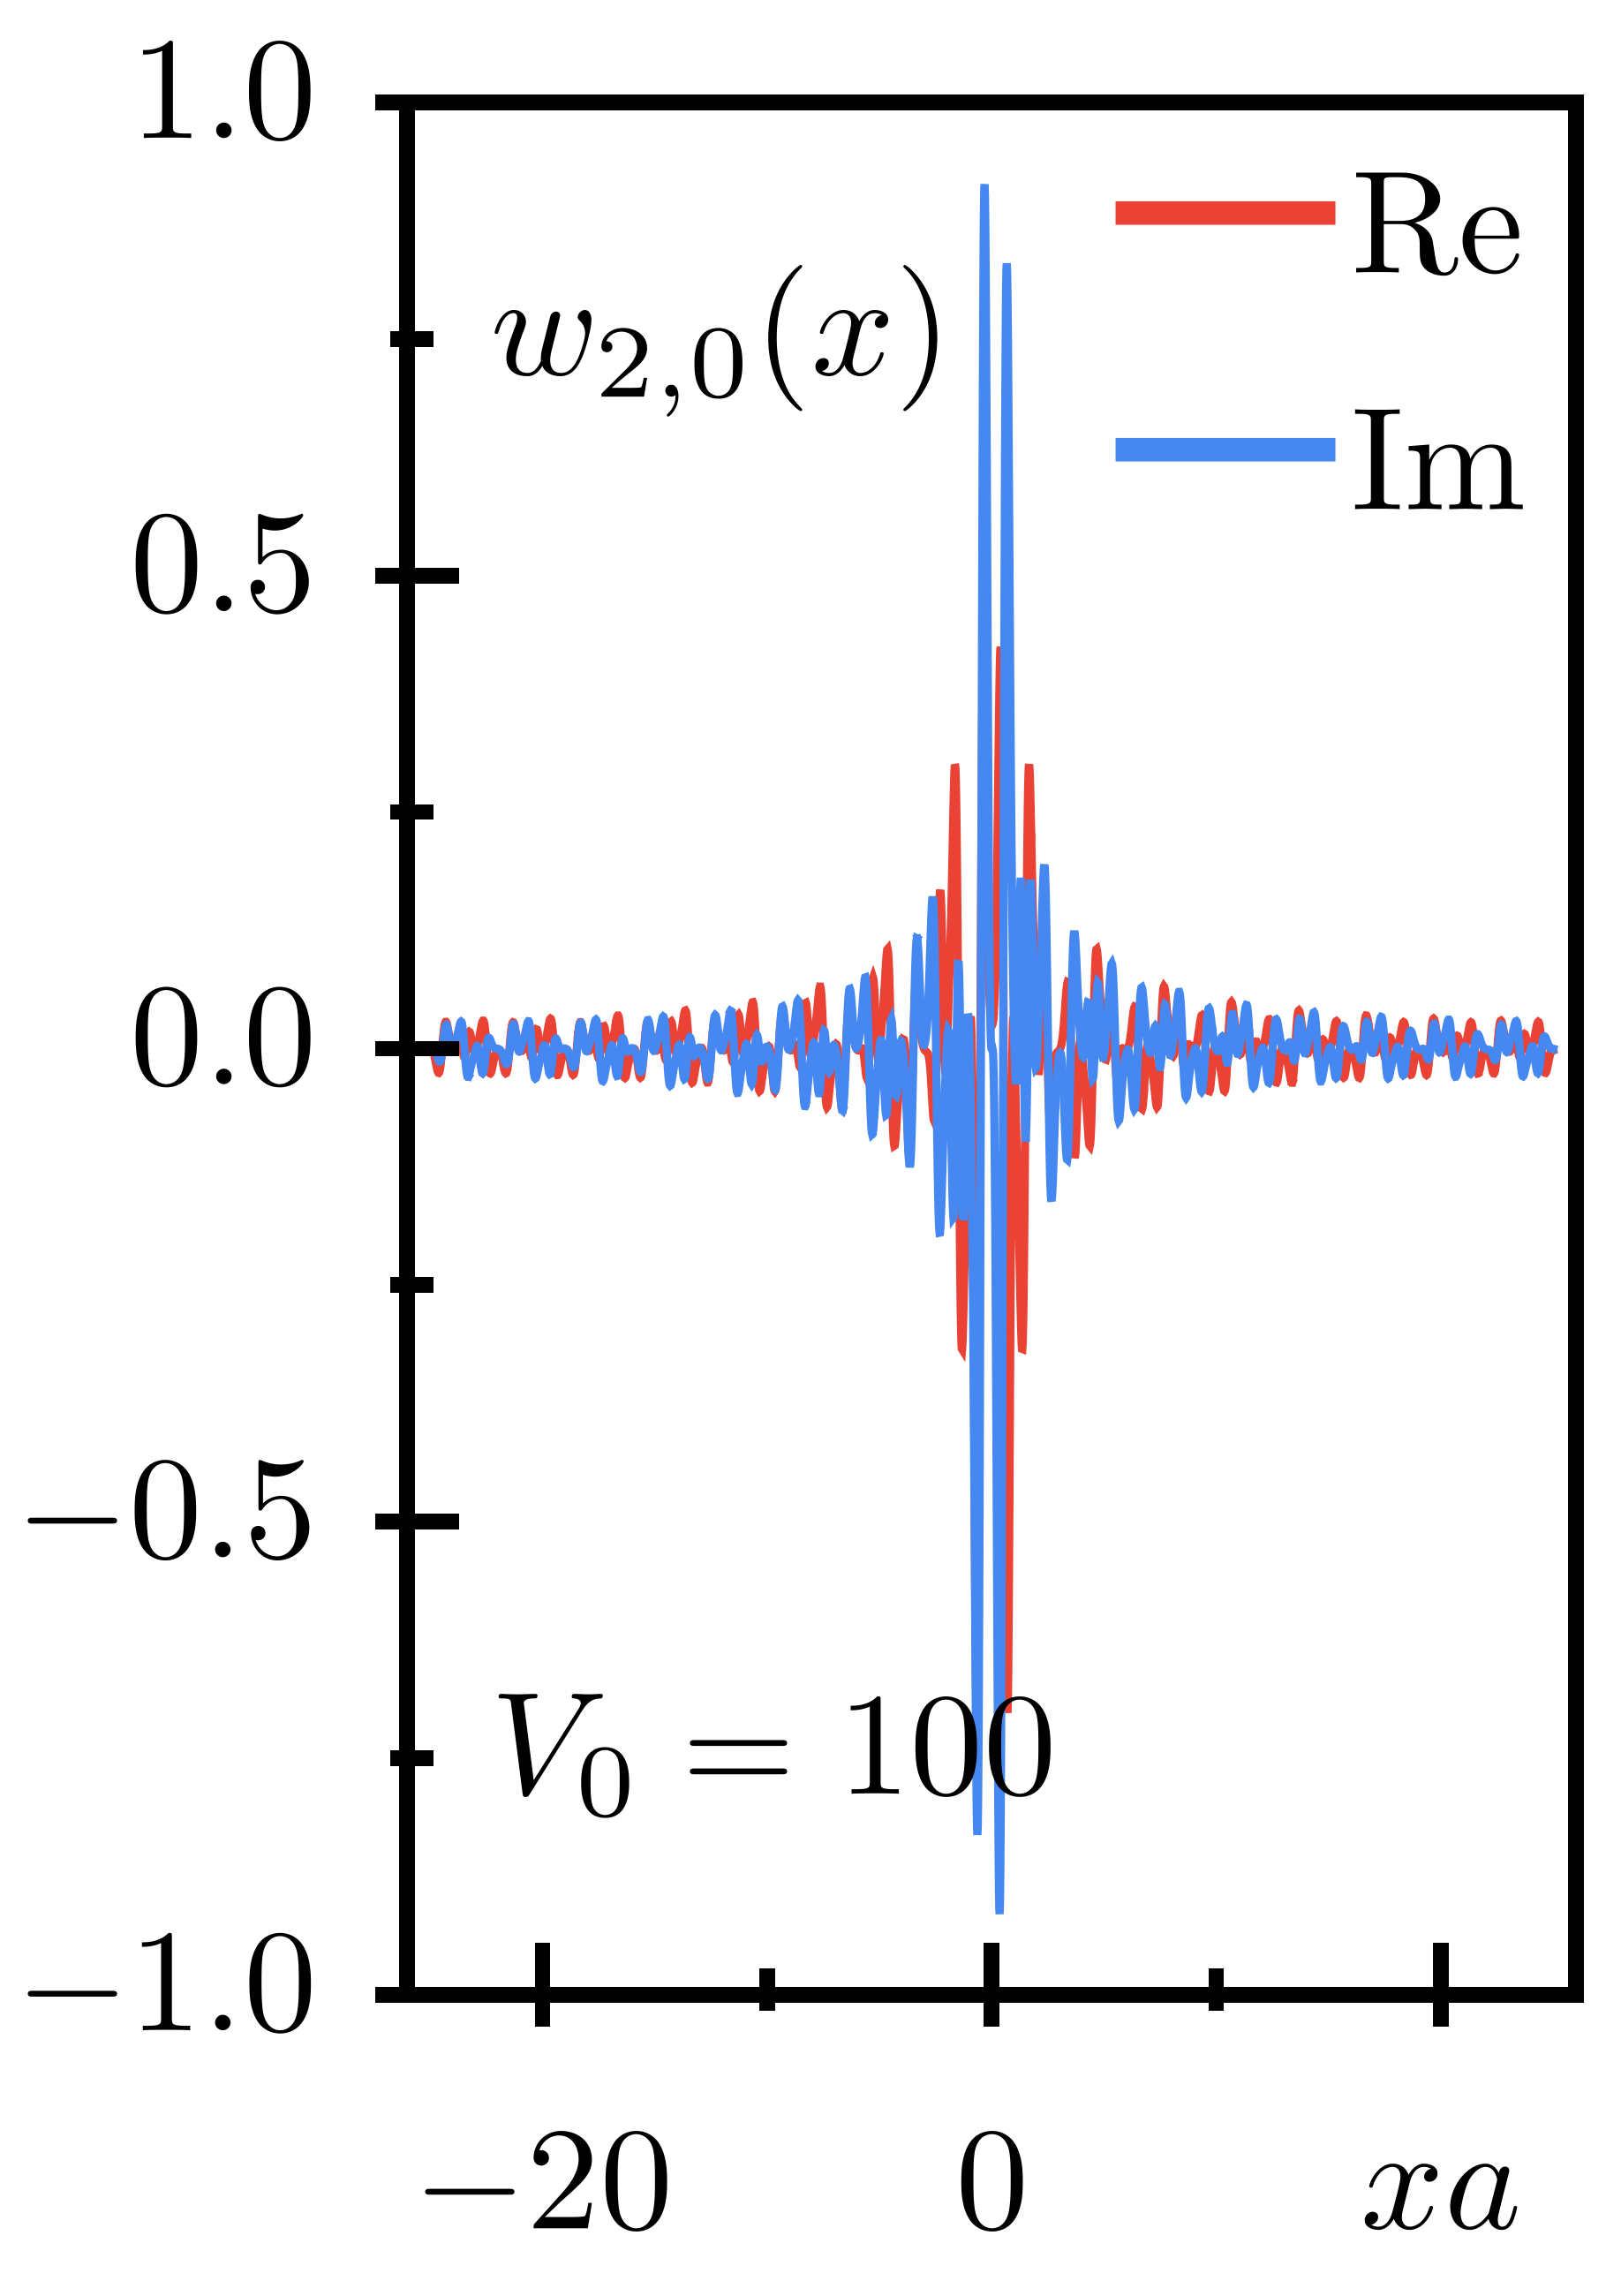
\includegraphics{figures/wannier2_100.png}}\\
    \caption{Example Wannier functions of the first two bands for a periodic potential of the form $V_{ae}(x)=V_0\cos(2\pi/ax)$ for different potential depth. The integration of the Bloch states was performed by assuming a periodicity over $L=50$ lattice translations.}
    \label{fig:tight_binding_wanniers}
\end{figure}

For this purpose, we assume the problem of the single-particle Hamiltonian $\hat H_0$ to be fully solved, such that the Bloch states $\psi_{\alpha{\bm k}}$ diagonalize $\hat H_0$ and have energy eigenvalues $\varepsilon_{\alpha{\bm k}}$.
This allows to introduce the Wannier basis -- a localized basis composed of the Bloch states and defined as
\begin{align}
    \ket{w_{\alpha{\bm R}}} = \frac1{\sqrt N}\sum_{\bm k}\re^{-\ri{\bm k}{\bm R}}\ket{\psi_{\alpha{\bm k}}}.
    \label{eq:wannier_states}
\end{align}
Note that every momentum-resolved Bloch function can be multiplied with a complex phase without changing its properties.
This naturally provides a gauge freedom to optimize the Wannier function's properties -- for instance, the construction of a maximally localized basis~\cite{Marzari2012}.
Without going into detail about optimizing Wannier functions, I want to present a basic visualization of these localized states.
For this purpose, let us consider a cosine periodic potential
\begin{align}
    V_{ae}(x) = V_0\cos\brlr{\frac{2\pi}a x}
\end{align}
which yields a particular easy (a tridiagonal Toeplitz) matrix equation for the Bloch vectors presented in \cref{eq:periodic_lattices_numerics}.
To obtain the Wannier functions, we gauge every Bloch function to be purely real at $x=0$, resulting in the examples displayed in \cref{fig:tight_binding_wanniers}.

The existence of localized Wannier states is translated to the language of second quantization by the notion that transformations between a Bloch and Wannier basis are always unitary.
Hence, annihilation and creation operators of Wannier and Bloch states are set in relation by
\begin{align}
    \hat a^\dag_{\alpha{\bm R}} = \frac1{\sqrt N}\sum_{\bm k}\re^{-\ri{\bm k}{\bm R}}\hat a^\dag_{\alpha{\bm k}},
    \quad
    \hat a^\dag_{\alpha{\bm k}} = \frac1{\sqrt N}\sum_{\bm R}\re^{+\ri{\bm k}{\bm R}}\hat a^\dag_{\alpha{\bm R}}.
    \label{eq:wannier_states_2}
\end{align}
Since the non-interacting Hamiltonian is diagonal in the Bloch basis, they are the eigenfunctions with energies $\varepsilon_{\alpha{\bm k}} = \int\rd^dr\, \psi_{\alpha{\bm k}}^* \hat H_0 \psi_{\alpha{\bm k}} = \frac1N\sum_{\bm R,\bm R'}\re^{\ri\bm k(\bm R'-\bm R)}\int\rd^dr\, w_{\alpha{\bm R}}^* \hat H_0 w_{\alpha{\bm R'}}$.
In particular, the Hamiltonian is readily cast into the localized basis according to
\begin{align}
    \hat H_0
    =
    \varepsilon_{\alpha{\bm k}}\hat a^\dag_{\alpha{\bm k}}\hat a^\pdag_{\alpha{\bm k}}
    \overset{\text{\cref{eq:wannier_states_2}}}{=}
    \frac1N
    \re^{\ri{\bm k}\brlr{{\bm R}-{\bm R'}}}
    \varepsilon_{\alpha{\bm k}}
    \hat a^\dag_{\alpha{\bm R}}\hat a^\pdag_{\alpha{\bm R'}}
    =
    T_{\alpha,i,j}
    \hat a^\dag_{\alpha{\bm R}_i}\hat a^\pdag_{\alpha{\bm R}_j},
    \label{eq:tight_binding_hamiltonian}
\end{align}
for which I conveniently use the sum convention.
The matrix $T_{\alpha}$ contains all amplitudes of transition processes between two lattice centers, to be determined through the dispersion relation of the $\alpha$-band
\begin{align}
    T_{\alpha,i,j} \coloneqq \frac1N\sum_{\bm k}\re^{\ri{\bm k}\brlr{{\bm R}_i-{\bm R}_j}}\varepsilon_{\alpha{\bm k}} = \frac1N\sum_{\bm k}\re^{\ri{\bm k}\brlr{{\bm R}_i-{\bm R}_j}}\int\rd^dr\, \psi_{\alpha{\bm k}}^* \hat H_0 \psi_{\alpha{\bm k}}.
\end{align}
On an intuitive level, the tight binding Hamiltonian denotes quantum particles hopping between lattice sites, connected through the matrix elements $T_{\alpha,i,j}$.
Without quantitative computations of the transition probabilities, we can fix the matrix to $T_{\alpha,i,j}=\sum_rt_{\alpha r}\delta_{i-r,j} + \hc$ with some constants $t_{\alpha r}$.
The relation \cref{eq:tight_binding_hamiltonian} has strong implications on the analytic form of the dispersion relation $\varepsilon_{\alpha{\bm k}}$ -- it is fully determined through the geometry of the crystal lattice.
For instance, one-dimensional lattices with single atom unit cells and lattice spacing $a$ have the particularly easy solution
\begin{align}
    \varepsilon_{\alpha k} = \sum_r 2t_{\alpha r}\cos(r ka).
    \label{eq:1D_tight_binding_dispersion}
\end{align}
Note that this equation is consistent with the Kronig-Penney dispersion relation in the tight-binding limit, presented in \cref{eq:kronig_penney_tight_binding_dispersion}.
In higher dimensions, the evaluation of the dispersion relation may become lengthy, but remains always analytic.

Oftentimes, a single-band approximation is established to fix (and drop) the band index $\alpha$.
This situation may be achieved in case the bottom band is sufficiently separated from the second.
In the Kronig-Penney model, this corresponds to $V_0\gg \hbar^2/(mab)$ with particle mass $m$, lattice constant $a$ and potential width $b$.
For the emergence and discussion of such an approximation in case of ultracold atoms trapped in optical lattices, I refer to~\cite{Jaksch1998,Bloch2008,Buechler2010,Mazza2012}.
Note that the single band approximation naturally fails do describe effects like orbital-selective Mott transitions which require at least two inequivalent bands~\cite{Anisimov2002,vanDongen2005}.

A corresponding two-body interaction $\hat V$ in the single-band approximation reads
\begin{align}
    \hat V = \frac12\sum_{i,i',j,j'}V_{i,i',j,j'}\hat a^\dag_{{\bm R}_i}\hat a^\dag_{{\bm R}_{i'}}\hat a^\pdag_{{\bm R}_j}\hat a^\pdag_{{\bm R}_{j'}}.
\end{align}
The matrix elements of the interaction are given by the integral expressions
\begin{align}
    V_{i,i',j,j'} = \int\rd^dr\int\rd^dr'\,w^*_{{\bm R}_i}({\bm r})w^*_{{\bm R}_{i'}}({\bm r}')w_{{\bm R}_j}({\bm r}')w_{{\bm R}_{j'}}({\bm r})V({\bm r-\bm r'}).
    \label{eq:two_body_interaction_transition_rates}
\end{align}
The explicit determination of the matrix elements requires knowledge of the form of the Wannier states which is an active field of research on its own.
However, these states are localized and as such the transition rate integrals are short-ranged in most cases.
In one dimension, it is often sufficient to account for transitions and interactions up to nearest neighbors
\begin{align}
    T_{i,j} \approx t_0\delta_{i,j} + t_1\delta_{i-1,j}+t_1^*\delta_{i+1,j},
    \quad
    V_{i,i',j,j'} \approx U\delta_{i,j'}\delta_{i',j}\delta_{i,i'} + V\delta_{i,j'}\delta_{i',j}(\delta_{i-1,i'}+\delta_{i+1,i'}).
\end{align}
Note that in case the particle has some flavor (e.g. spin), the kinetic terms of $\hat H_0$ typically act in a diagonal manner.
On the contrary, the two-body interaction allows for both intra-flavor and inter-flavor scattering processes.

We are at liberty to slightly simplify the notation and arrive at the family of single-orbital Hubbard-type models, written in second quantization
\begin{align}
    \hat H_{\rm Hubbard} = \sum_{i,s}\brlr{t_1 \hat a^\dag_{i,s}\hat a^\pdag_{j+1,s} + \hc} + \frac U2\sum_{i,s,s'}\hat n_{i,s}\hat n_{i,s'} + V\sum_{i,s,s'}\hat n_{i,s}\hat n_{i+1,s'}.
    \label{eq:hubbard_hamiltonian}
\end{align}
The operator $\hat a_{i,s}$ annihilates a Wannier state of flavor $s$, localized around the $i$'th lattice position.
In most cases, $t_1 = -t$ with $t>0$, which is also physically motivated to confine the minimum of the dispersion to $k=0$.
The validity of the single-band approximation for real materials requires small interaction amplitudes compared to the band gap between the first and second Bloch band.

If the matrix $T$ defines a lattice grid with loops, complex transition amplitudes give rise to nontrivial fluxes penetrating the lattice which may alter the underlying physics.
The famous Peierls' substitution approximates the effect of a uniform magnetic field, in which case the Hamiltonian follows the principle of minimal coupling
\begin{align}
    \hat H_0 = \frac{\hat{\bm p}^2}{2m}+V_{ae}(\bm r)\rightarrow \frac{\brlr{\hat{\bm p} - q\bm A(\bm r)}^2}{2m}+V_{ae}(\bm r),
\end{align}
and $q$ denotes the electric charge of the particle.
Consider now the rescaled Wannier functions
\begin{align}
    w'_{\alpha\bm R} = \re^{\ri\frac q\hbar G_{\bm R}}w_{\alpha\bm R},
    \quad
    \psi'_{\alpha\bm k} = \frac1N\sum_{\bm R}\re^{\ri\bm k\bm R}w'_{\alpha\bm R}
\end{align}
in which $G_{\bm R}(\bm r) = \int_{\bm R}^{\bm r}\bm A(\bm r')\cdot\rd \bm r'$ is a lattice-position and position dependent phase.
In certain situations, this provides a neat substitution to treat the troublesome $\hat{\bm p}\bm A$ term.
In fact, $\bm\nabla G_{\bm R}(\bm r) = \bm A(\bm r) + \int_0^1\rd\lambda\lambda (\bm r-\bm R)\times\bm B(\bm R+\lambda(\bm r-\bm R))$ with magnetic field $\bm B=\bm\nabla\times\bm A$~\cite{Luttinger1951}.
To observe the influence of the magnetic field, the transition elements between different Wannier states have to be computed, i.e.
\begin{align}
    % \varepsilon_{\alpha\bm k}
    % =
    % \frac1N\sum_{\bm R,\bm R'}\re^{\ri\bm k(\bm R'-\bm R)}
    % \int\rd^d r
    %     w_{\alpha\bm R}^*
    %     \re^{-\ri\frac q\hbar\int_{\bm R}^{\bm r}\bm A(\bm r')\cdot\rd \bm r'}
    %     \brlr{\frac{\brlr{\hat{\bm p}-q\bm A}^2}{2m}+V_{ae}}
    %     w_{\alpha \bm R'}
    %     \re^{\ri\frac q\hbar\int_{\bm R'}^{\bm r}\bm A(\bm r')\cdot\rd \bm r'}
    % \\
    % =
    % \frac1N\sum_{\bm R,\bm R'}\re^{-\ri\frac q\hbar\int_{\bm R}^{\bm R'}\bm A(\bm r')\cdot\rd \bm r'}\re^{\ri\bm k(\bm R'-\bm R)}
    % \int\rd^d r
    %     \re^{\ri\frac q\hbar\Phi_{\bm R,\bm R'}(\bm r)}
    %     w_{\alpha\bm R}^*
    %     \brlr{\frac{\brlr{\hat{\bm p}-q\bm A+q\bm\nabla G_{\bm R'}}^2}{2m}+V_{ae}}
    %     w_{\alpha \bm R'}
    T_{\alpha,i,j}
    =
    \int\rd^d r
        w_{\alpha\bm R_i}^*
        \re^{-\ri\frac q\hbar G_{\bm R_i}}
        \brlr{\frac{\brlr{\hat{\bm p}-q\bm A}^2}{2m}+V_{ae}}
        w_{\alpha \bm R'}
        \re^{\ri\frac q\hbar G_{\bm R_j}}
    \\
    =
    \re^{-\ri\frac q\hbar\int_{\bm R_i}^{\bm R_j}\bm A(\bm r')\cdot\rd \bm r'}
    \int\rd^d r
        \re^{\ri\frac q\hbar\Phi_{\bm R_i,\bm R_j}(\bm r)}
        w_{\alpha\bm R_i}^*
        \brlr{\frac{\brlr{\hat{\bm p}-q\bm A+q\bm\nabla G_{\bm R_j}}^2}{2m}+V_{ae}}
        w_{\alpha \bm R_j},
\end{align}
in which $\Phi_{\bm R_i,\bm R_j}(\bm r) = \oint_{\bm R_j\rightarrow\bm r\rightarrow\bm R_i}\bm A(\bm r')\cdot\rd \bm r'$ is the flux through the plaquette spanned by $\bm R_i, \bm R_j$ and $\bm r$.
% Now the locality of the Wannier functions is exploited, and the variation of the vector potential on the atomic scale is such that $\nabla G_{\bm R'}(\bm r)\approx\bm A(\bm r)$, which leads to
% \begin{align}
%     \varepsilon_{\alpha\bm k}
%     \approx
%     \frac1N\sum_{\bm R,\bm R'}\re^{\ri\frac q\hbar\int_{\bm R'}^{\bm R}\bm A(\bm r')\cdot\rd \bm r'}\re^{\ri\bm k(\bm R'-\bm R)}
%     \int\rd^d r
%         \re^{\ri\frac q\hbar\Phi_{\bm R,\bm R'}(\bm r)}
%         w_{\alpha\bm R}^*
%         \hat H_0
%         w_{\alpha \bm R'}
%     .
% \end{align}
Expanding to first order in $B=|\bm B|$, the transition elements are dressed with a complex phase factor and result to the famously known Peierls approximation
\begin{align}
    T_{\alpha,i,j}'=\re^{\ri\frac q\hbar\int_{\bm R_j}^{\bm R_i}\bm A(\bm r')\cdot\rd\bm r'}T_{\alpha,i,j}+\mathcal O(B).
\end{align}
The transition elements correspond to the change in the Berry phase on the lattice scale~(for a discussion and implications of this effect, see \cref{ch:topological_phases_of_matter}).
Note that the amplitudes of the transitions are altered as well, which must be considered in the implementation of real experiments~\cite{Alexandrov1991}.

Perhaps the most successful description of electrons in solids is band theory -- based on screened many-body interactions described by effective one-body potentials.
This results in a form of \cref{eq:hubbard_hamiltonian} without density-density interactions such that a diagonalization of the hopping matrix $T$ solves the problem.
However, due to its intrinsic single-particle character, band theory cannot reliably capture truly many-body features such as band magnetism or Mott-to-metal-insulator transitions.
This motivates the study of Hubbard-type models: despite being a brutal simplification of the true two-body interaction, they are the simplest systems that provide an explanation of such interaction-driven features.
Despite its apparent innocence, there is no universal treatment of Hubbard models in general.
In one spatial dimension, the Hamiltonian can be solved analytically using the Bethe Ansatz and thus falls in the category of being ``integrable''~\cite{Essler2005}.
In general, Bethe Ansatz integrability is a fragile property and even slight perturbations will break it.
The models we study in the next chapters, albeit closely related to the one-dimensional Hubbard model, do not categorize as integrable due to the presence of additional terms that break some of its fundamental symmetries (e.g. the conservation of the particle flavor).
This motivates the use of alternative methods to study the properties of interacting tight binding models.
One of the most prominent and useful analytic concepts in one dimension is the theory of Luttinger liquids (paired with renormalization group theory) which approximates the microscopic model in the low temperature limit.
%
%
%%%%%%%%%%%%%%%%%%%%%%%%%%%%%%%%%%%%
\section{Tomonaga-Luttinger liquids}
\label{sec:tomonaga_LL}
%%%%%%%%%%%%%%%%%%%%%%%%%%%%%%%%%%%%
Tomonaga-Luttinger liquids are gapless interacting states of matter appearing in many one-dimensional quantum systems.
Their understanding was formalized at the beginning of the '80s by Duncan Haldane~\cite{Haldane1981} through the application of a technique called Abelian bosonization.
It was understood that the low-lying excitations of these fermionic interacting models can be approximated with free bosons.
In this section, I give a basic overview of the mapping from spinless fermions to bosonic particle-hole excitations in the vicinity of the Fermi points.

The main interest here is to achieve an effective model in one dimension capturing the relevant degrees of freedom at low temperatures and low energies.
For that purpose, let me start with the free fermionic 1D Hamiltonian $\hat H_0$ denoted by the following (diagonal) representation in momentum space
\begin{align}
    \hat H_0 = \sum_k \frac{(\hbar k)^2}{2m}\hat n_k
    \label{eq:hamiltonian_free_particles}
\end{align}
with dispersion relation $\varepsilon_k =\frac{k^2}{2m}$ depicted in \cref{fig:1D_quadratic_dispersion}.
\begin{figure}
    \centering
    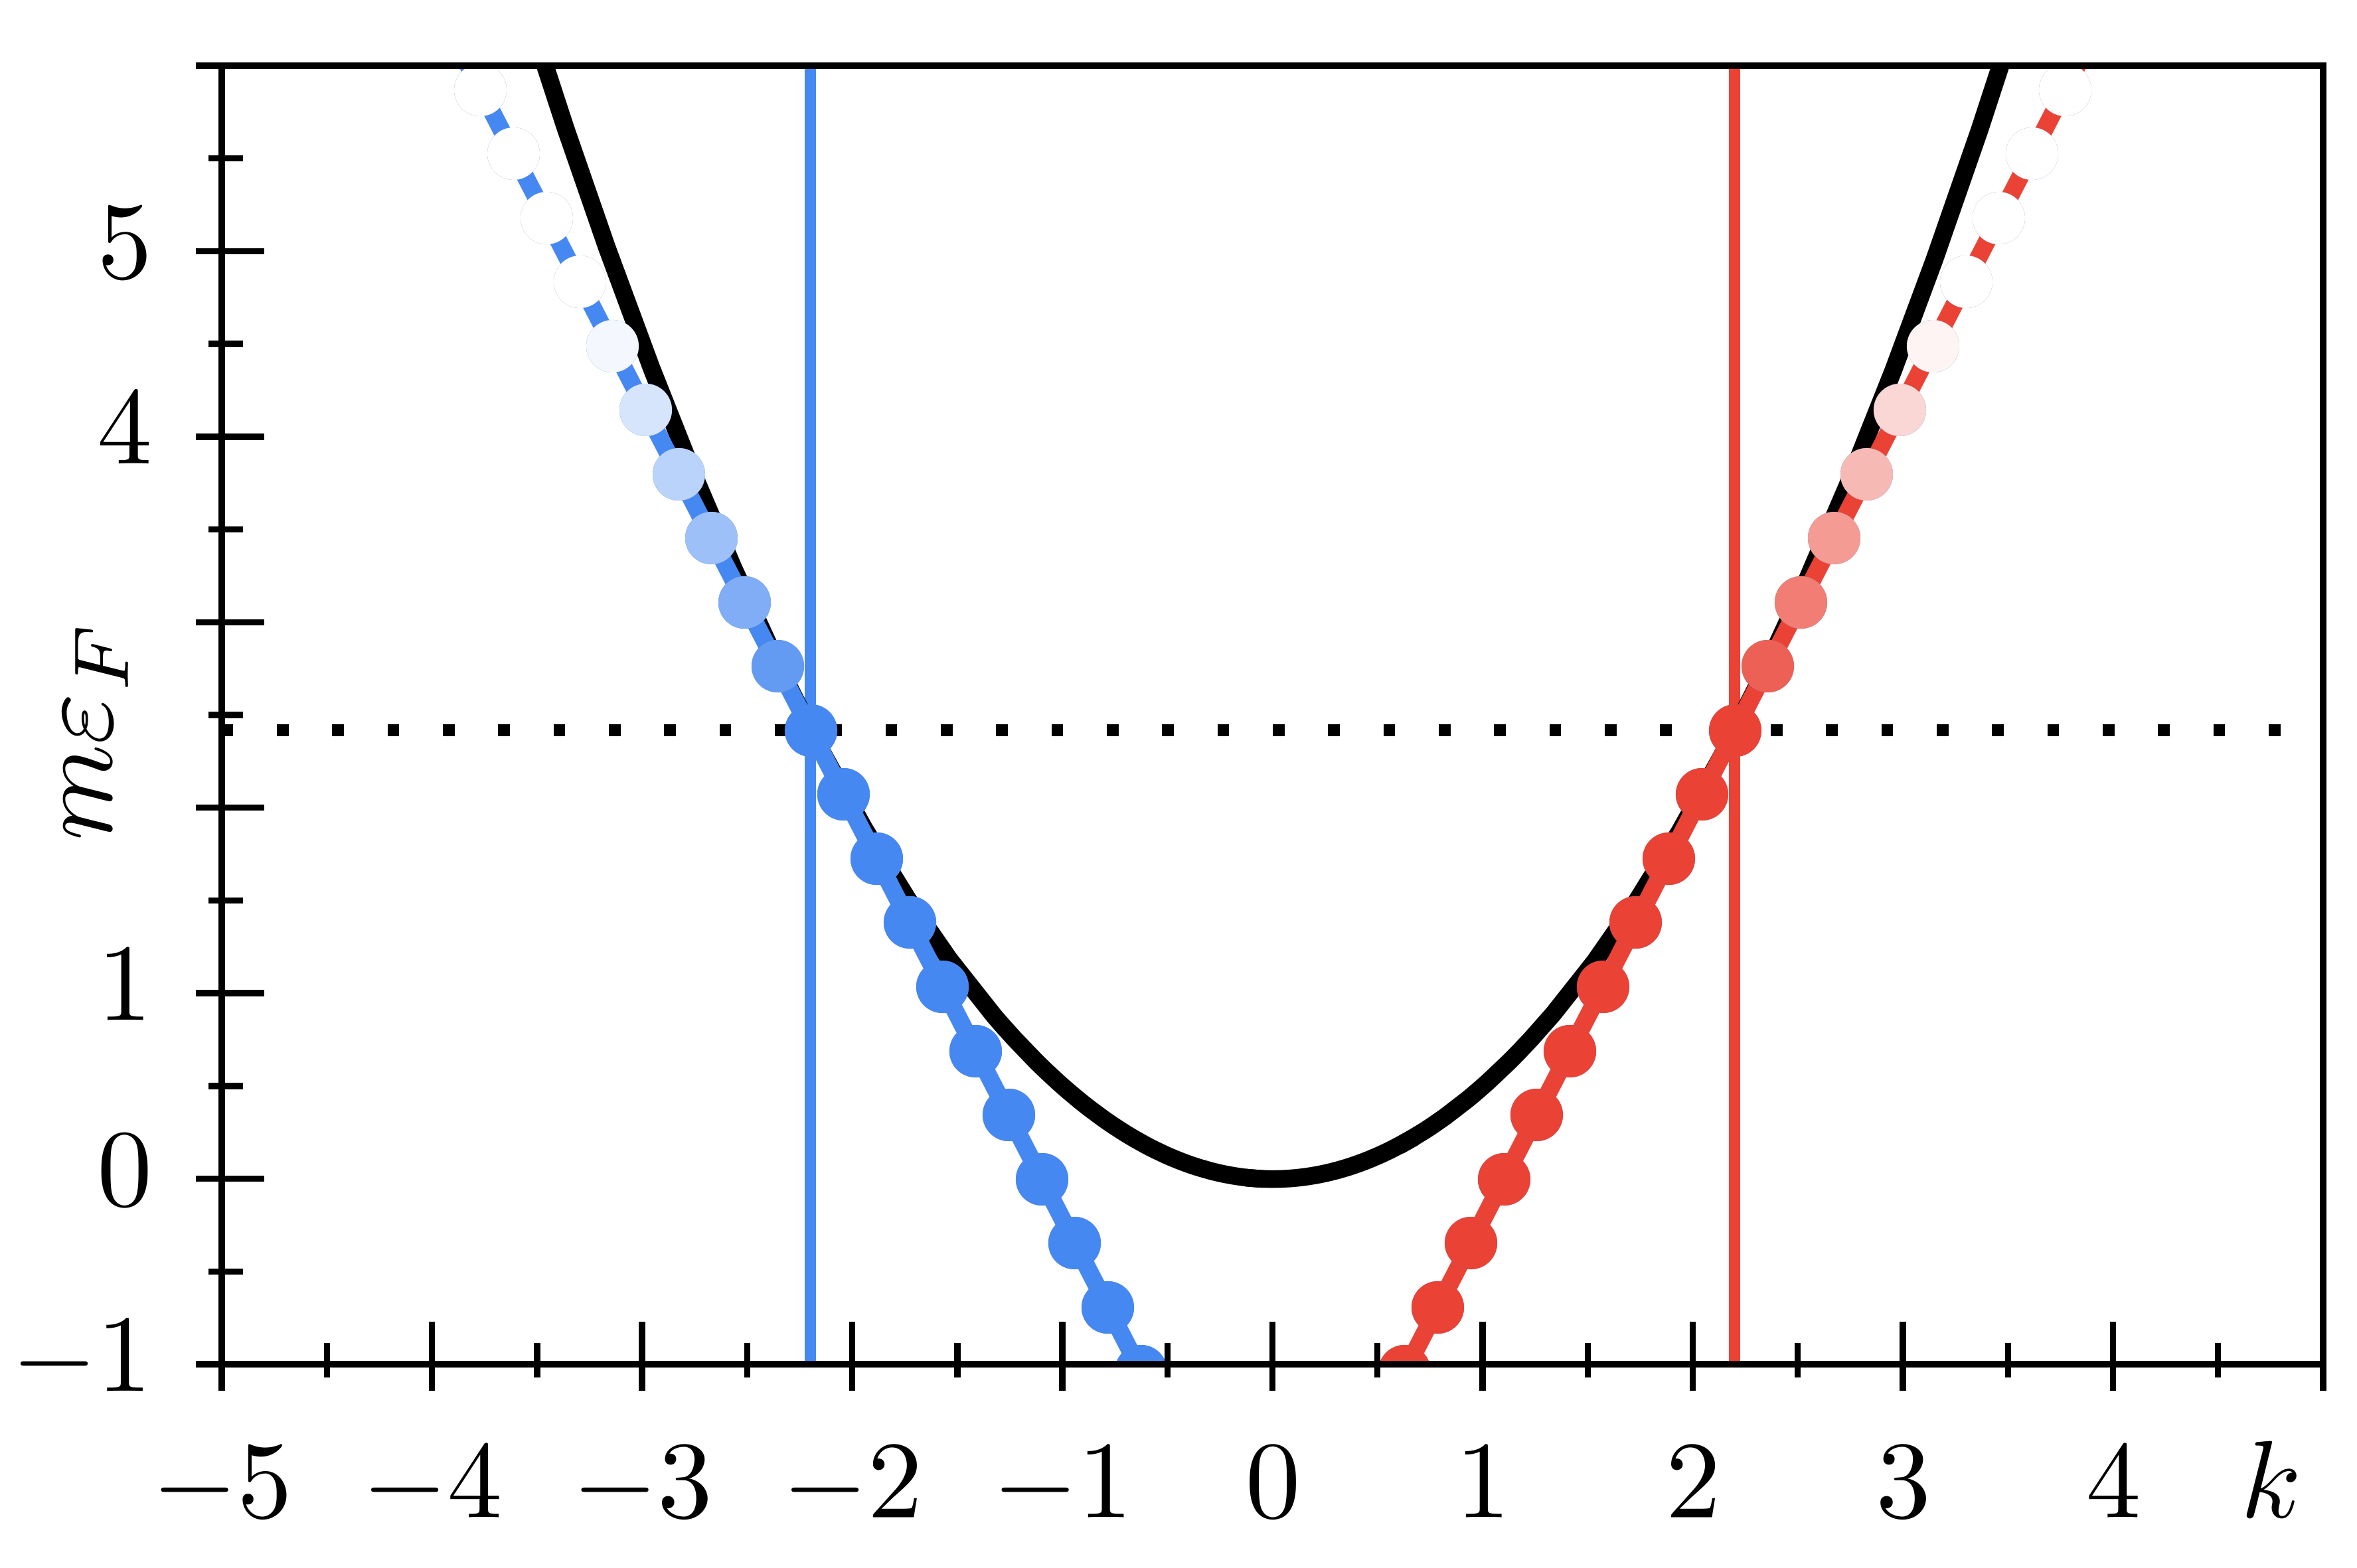
\includegraphics{figures/1D_quadratic_dispersion.png}
    \caption{Quadratic dispersion relation with approximations close to the Fermi energy $\varepsilon_F$.}
    \label{fig:1D_quadratic_dispersion}
\end{figure}
Close to the Fermi energy $\varepsilon_F\coloneqq\varepsilon_{\pm k_F}$, one may linearize the free dispersion to obtain a system of two different species
\begin{align}
    \hat H_0
    &\approx \sum_k \hbar^2\brlr{\varepsilon_F \pm \frac{k_F}{m}(k\mp k_F)}\hat n_k
    \\
    &= \sum_q \hbar^2\brlr{\varepsilon_F + \frac{k_F}{m}q\brlr{\hat n_{q+k_F}-\hat n_{q-k_F}}}
    \approx \sum_{q} v_F \hbar q \brlr{\hat c^\dag_{q,R}\hat c^\pdag_{q,R} - \hat c^\dag_{q,L}\hat c^\pdag_{q,L}},
    \label{eq:dispersion_linearization}
\end{align}
which implies a restriction of $q$ to a small window $|q|<\Gamma\ll k_F$ beyond which \cref{eq:dispersion_linearization} is considered invalid.
Note the introduction of the so-called right and left operators $\hat c_{R/L,q}$ which annihilate particles propagating to the left/right with Fermi velocity $\pm v_F=\hbar k_F/m$.

For the next part, it is convenient to investigate the local density in momentum space, i.e.
\begin{align}
    \hat n(x) = \hat c^\dag_x \hat c^\pdag_x = \frac1L\sum_{k,q}\re^{-\ri x q}\hat c^\dag_{k+q}\hat c^\pdag_{k}.
    \label{eq:local_density}
\end{align}
$\hat n(x)$ thus creates a superposition of particle-hole plane waves with characteristic wavelength $q^{-1}$.
The bare creation of particle-hole pairs is defined through the density operator
\begin{align}
    \hat \rho_{-q}\coloneqq \sum_k \hat c^\dag_{k-q}\hat c^\pdag_{k}.
\end{align}
Note further that $\hat\rho_q^\dag = \hat\rho_{-q}$.
By confining the theory close to the Fermi points, there are only two different classes of particle-hole excitations with $q\approx 0$ and $q\approx\pm2k_F$.
The long-wavelength excitations $q\approx0$ are particle-hole pairs of the same species (left or right movers), and excitations of $q\approx\pm2k_F$ are particle-hole pairs of a mixture of the two.
This implies drastic consequences for the relevant action of operators, which we will see in the following.
Let us note here that the density operator of the left/right species $\hat\rho_{\tau,q}$, $\tau\in\{L,R\}$ applied to a Fermi sea creates stable particle-hole excitations (i.e. particles and holes propagate with the same velocity $\pm v_F$) and can thus be used to construct a complete basis of the subspace $\FS^N$ -- for this rather dry discussion, I refer to~\cite{vonDelft1998}.
The consequences of the approximation in \cref{eq:dispersion_linearization} is easily understood for the single-particle operators
\begin{align}
    \hat c^\dag_x = \frac1{\sqrt L}\sum_k \re^{-\ri k x}\hat c^\dag_k \approx \frac1{\sqrt L}\sum_{|q|<\Gamma}\re^{-\ri (q+k_F) x}\hat c^\dag_{q,R} + \re^{-\ri (q-k_F) x}\hat c^\dag_{q,L}
    \label{eq:confinement_creation_annihilation}
\end{align}
which is then used to find the local density
\begin{align}
    \hat n(x)
    &\approx \frac1L\sum_{q,q'}\brlr{\re^{-\ri (q+k_F) x}\hat c^\dag_{R, q} + \re^{\ri (k_F-q) x}\hat c^\dag_{L, q}}\brlr{\re^{\ri (k_F+q') x}\hat c^\pdag_{R, q'} + \re^{-\ri (k_F-q') x}\hat c^\pdag_{L, q'}},
    \\
    &= \hat \rho_R(x) + \hat \rho_L(x) + \re^{-2\ri k_Fx}\hat c^\dag_{R}(x)\hat c^\pdag_{L}(x) + \re^{2\ri k_Fx}\hat c^\dag_{L}(x)\hat c^\pdag_{R}(x).
    \label{eq:local_density_approximation}
\end{align}
The first two terms correspond to the $q\approx0$ part of the density, and scattering occurs on the same side of the dispersion relation.
The last two terms scatter right with left movers and transfer particles from one side to the other, which appear at $q\approx\pm2k_F$.

We now turn to an arbitrary two-body interaction of the form~\cref{eq:two_point_interaction} which reads
\begin{align}
    \hat V
    % &= \frac12\int\rd x'\int\rd x V(x'-x)c^\dag(x')c^\dag(x)c^\pdag(x)c^\pdag(x')
    % \\
    &= \frac12\int\rd r\int\rd x V(r)\hat c^\dag(r+x)\hat c^\dag(x)\hat c^\pdag(x)\hat c^\pdag(r+x),
    \\
    &= \frac1{2L^2}\sum_{kk'll'}\int\rd r\int\rd x V(r)\re^{-\ri r(k-l')}\re^{-\ri x(k-l'+k'-l)}\hat c^\dag_k\hat c^\dag_{k'}\hat c^\pdag_l\hat c^\pdag_{l'},
    % \\
    % &= \frac1{2L}\sum_{kk'lq}\int\rd r V(r)\re^{-\ri rq}\delta_{l,k'+q}c^\dag_kc^\dag_{k'}c^\pdag_lc^\pdag_{k-q}
    \\
    &= \frac1{2L}\sum_{kk'q}V(q)\hat c^\dag_k\hat c^\dag_{k'}\hat c^\pdag_{k'+q}\hat c^\pdag_{k-q}
    = \frac1{2L}\sum_{q}V(q)\hat\rho_q\hat\rho^\dag_{q} - \mu.
    \label{eq:two_body_interaction_momentum_space}
\end{align}
The last term is just a constant $\mu = \frac N{2L}\sum_qV(q)$ and can thus be neglected.
By imposing that relevant contributions act close to the Fermi energy involving only momenta in the interval $|k|\in[k_F-\Gamma,k_F+\Gamma]$, we can split the sum in two contributions, one involving scattering processes at small and the other scattering at large momenta
\begin{align}
    \hat V \approx \frac1{2L}\brlr{\sum_{q\approx0}V(q)\hat\rho_{q}\hat\rho^\dag_{q} + \sum_{q\approx2k_F}V(q)\hat\rho_{q}\hat\rho^\dag_{q}}.
\end{align}
% For the study presented in \cref{drude_increased1}, it is important to note that the amplitude of the two different $q\approx0$ processes, denoted by $V(q\approx0)$, is equal and independent of the form of the interaction.
An intuitive classification of the scattering processes is given in~\cref{fig:scattering_processes}.
\begin{figure}
    \centering
    \subfigure[]{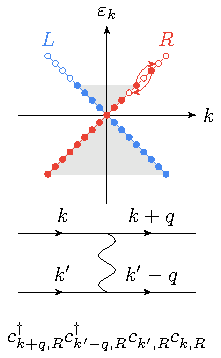
\includegraphics[width=0.328\textwidth]{figures/g4_right.pdf}}
    \subfigure[]{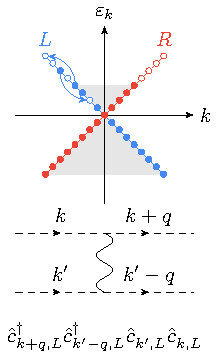
\includegraphics[width=0.328\textwidth]{figures/g4_left.pdf}}
    \subfigure[]{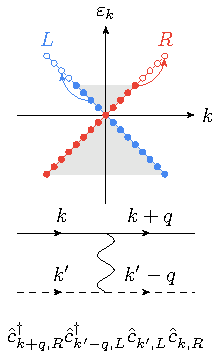
\includegraphics[width=0.328\textwidth]{figures/g2.pdf}}
    \subfigure[]{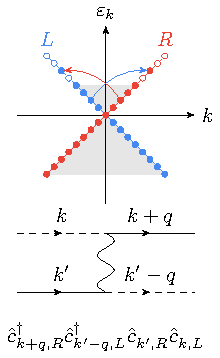
\includegraphics[width=0.328\textwidth]{figures/g1.pdf}}
    \subfigure[]{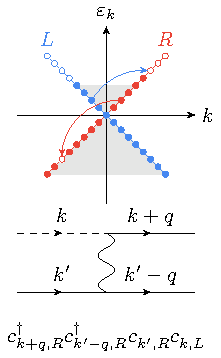
\includegraphics[width=0.328\textwidth]{figures/g13.pdf}}
    \subfigure[]{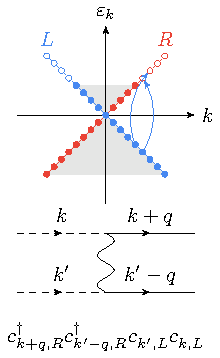
\includegraphics[width=0.328\textwidth]{figures/g22.pdf}}
    \caption{Relevant scattering processes of a generic density-density interaction in one-dimensional quantum systems. (a)/(b) The depicted scattering is commonly referred to as ``forward scattering'' $g_4$ process ($4$ right/left operators, $q\approx0$), (c) as ``backscattering'' $g_2$ process (containing $2$ pairs of right and left operators, $q\approx0$) and (d) as $g_1$ process with momentum transfer $q\approx 2k_F$. Other possible scatterings like the ones depicted in (e) and (f) require the existence of high-energy excitations and are thus exponentially suppressed at low temperatures.}
    \label{fig:scattering_processes}
\end{figure}
This simple argumentation allows to consider only the most relevant processes at low temperatures/energies, i.e. those presented in panels (a) - (d).
We will call those processes forward scattering
\begin{align}
    g_4\sum_{k,k',q}\hat c^\dag_{k+q,\tau}\hat c^\dag_{k'-q,\tau}\hat c^\pdag_{k',\tau}\hat c^\pdag_{k,\tau} = g_4 \sum_q\hat\rho^\pdag_{q,\tau}\hat\rho^\dag_{q,\tau},
\end{align}
backscattering
\begin{align}
    g_2\sum_{k,k',q}\hat c^\dag_{k+q,\tau}\hat c^\dag_{k'-q,\overline\tau}\hat c^\pdag_{k',\overline\tau}\hat c^\pdag_{k,\tau} = g_2\sum_q \hat\rho^\pdag_{q,\tau}\hat\rho^\dag_{q,\overline\tau}
\end{align}
and $g_1$ scattering
\begin{align}
    g_1\sum_{k,k',q} \hat c^\dag_{k+q,\tau}\hat c^\dag_{k'-q,\overline\tau}\hat c^\pdag_{k',\tau}\hat c^\pdag_{k,\overline\tau}.
\end{align}
Note that we are safely discarding possible constants on the right hand side of the previous equations.
The $g_1$ scattering of spinless fermions can be rewritten according to
\begin{align}
    \sum_{k,k',q}V(q)
    \hat c^\dag_{k+q,\tau}\hat c^\dag_{k'-q,\overline\tau}\hat c^\pdag_{k',\tau}\hat c^\pdag_{k,\overline\tau}
    =
    \sum_{k,k',q,q'}V(q) \delta_{q,q'-k+k'}
    \hat c^\dag_{k'+q',\tau}\hat c^\dag_{k-q',\overline\tau}\hat c^\pdag_{k',\tau}\hat c^\pdag_{k,\overline\tau}
    \\
    =
    -\sum_{k,k',q}V(k'-k+q)\hat c^\dag_{k+q,\tau}\hat c^\dag_{k'-q,\overline\tau}\hat c^\pdag_{k',\overline\tau}\hat c^\pdag_{k,\tau}
    \approx -V(2k_F)\sum_q\hat\rho^\pdag_{q,\tau}\hat\rho^\dag_{q,\overline\tau},
    \label{eq:umklapp_backscattering_equivalence}
\end{align}
which proofs that $g_1$ terms are up to a sign equivalent to backscattering terms in case of indiscernible particles.
Interestingly, the $2k_F$ components of forward scatterings can be reordered in the same manner\footnote{This is interesting because one is inclined to neglect the $2k_F$ forward scattering processes at first sight. The reordering demonstrates that $q\approx0$ are equivalent to $2k_F$ scatterings such that both have to be accounted for on equal grounds.}, such that we find the identity $g_4 = g_2 \approx V(0)-V(2k_F)$.
% Umklapp terms cannot be expressed in the density operators of the moving modes $\hat\rho_{q,\tau}$ and, for this reason, are discarded here\footnote{Later, we will see that the Umklapp term in the spinless case are ``marginal'' and can be disregarded under certain conditions.}.
Other processes like those depicted in \cref{fig:scattering_processes} (e) and (f) require the existence of high-energy excitations and can thus be neglected for the effective low temperature theory developed here.
In summary, we can express the interaction in terms of the density-density operators as
\begin{align}
    \hat V \approx \frac{\hbar}{2L}\sum_{q,\tau}\brlr{g_4\hat\rho^\pdag_{q,\tau}\hat\rho^\dag_{q,\tau} + g_2\hat\rho^\pdag_{q,\tau}\hat\rho^\dag_{q,\overline\tau}}
    =
    \frac{\hbar}{L}\sum_{q>0}
    \begin{pmatrix}
        \hat\rho^\pdag_{q,R} & \hat\rho^\pdag_{q,L}
    \end{pmatrix}
    \begin{pmatrix}
        g_4 & g_2 \\
        g_2 & g_4
    \end{pmatrix}
    \begin{pmatrix}
        \hat\rho_{-q,R} \\ \hat\rho_{-q,L}
    \end{pmatrix}
    .
    \label{eq:interaction_densities}
\end{align}
To proceed further, it will be useful to compute the commutation of the density operators
\begin{align}
    \commutator{\hat\rho_{q,\tau},\hat\rho_{q',\tau'}}
    =
    \delta_{\tau,\tau'}\sum_k\brlr{\hat c^\dag_{k+q,\tau}\hat c^\pdag_{k-q',\tau}-\hat c^\dag_{k+q+q',\tau}\hat c^\pdag_{k,\tau}}
    \approx
    -\sigma_\tau\delta_{\tau,\tau'}\delta_{q,-q'}\frac{qL}{2\pi}
    \label{eq:chiral_density_commutation}
\end{align}
in which $\sigma_\tau=\pm1$ for $\tau=R/L$, respectively, and the right hand side is obtained through a projection on the ground state\footnote{This is a reasonable approximation for small interactions only (as a result from a first order perturbative expansion).
For a more thorough discussion of \cref{eq:chiral_density_commutation}, see~\cite{Giamarchi2003}.
Although this approximation may turn out to be too rough for real systems, it allows to obtain the Luttinger liquid field theory.}.
We are now at liberty to define canonical bosonic operators representing the interaction degrees of freedom for $q>0$
\begin{align}
    \hat b^\dag_{+q} \coloneqq \sqrt\frac{2\pi}{qL}\hat\rho_{-q,L},
    \quad
    \hat b^\pdag_{+q} \coloneqq \sqrt\frac{2\pi}{qL}\hat\rho_{+q,L},
    \\
    \hat b^\dag_{-q} \coloneqq \sqrt\frac{2\pi}{qL}\hat\rho_{+q,R},
    \quad
    \hat b^\pdag_{-q} \coloneqq \sqrt\frac{2\pi}{qL}\hat\rho_{-q,R},
    \label{eq:canonical_bosonic_operators}
\end{align}
that satisfy the commutation relation $\commutator{\hat b_q^\pdag,\hat b_{q'}^\dag} = \delta_{q,q'}$.
Using \cref{eq:canonical_bosonic_operators} results in a familiar expression for the interaction written in \cref{eq:interaction_densities}, i.e.
\begin{align}
    \hat V \approx\sum_{q>0}\frac{\hbar q}{2\pi}
    \begin{pmatrix}
        \hat b_q & \hat b^\dag_{-q}
    \end{pmatrix}
    \begin{pmatrix}
        g_4 & g_2 \\
        g_2 & g_4
    \end{pmatrix}
    \begin{pmatrix}
        \hat b^\dag_q \\ \hat b_{-q}
    \end{pmatrix}
    .
    \label{eq:quadratic_interactions}
\end{align}
The interaction, originally quartic in the fermionic degrees of freedom, can be cast into a (quadratic) sum of bosonic operators which are the low-energy excitations of the original model.
All that is left to do is to cast the kinetic term into this new basis, which is actually a quite lengthy calculation if we were to approach it by brute-force.
There is an indirect reasoning through Schur's lemma~\cite{schur_neue_1905}: if two operators $\hat H$ and $\hat H'$ have identical commutation relations with all $\{c^\pdag_\alpha,c^\dag_\alpha\}$, then the two operators are equal up to an overall constant, which in this case can be interpreted as a chemical potential.
One can easily compute the commutator of the mover-density with the kinetic Hamiltonian
\begin{align}
    \commutator{\hat H_0, \hat\rho_{q,\tau}}
    =
    \sum_{p,\tau'}v_F\sigma_{\tau'}\hbar \commutator{\hat n_{p,\tau'},\hat\rho_{q,\tau}}
    =
    \sigma_\tau v_F \hbar q \hat\rho_{q,\tau}
\end{align}
and find its equivalent expression in bosonic degrees of freedom to be
\begin{align}
    \hat H_0' = \frac{\hbar \pi v_F}L\sum_{q,\tau}\hat\rho_{q,\tau}\hat\rho_{-q,\tau} = \frac{2\hbar\pi v_F}L\sum_{q>0,\tau}\hat\rho_{q,\tau}\hat\rho_{-q,\tau},
\end{align}
which can be verified through evaluation of
\begin{align}
    \commutator{\hat H_0',\hat\rho_{q,\tau}}
    \overset{\text{\cref{eq:recursive_commutation}}}{=}
    -\frac{\hbar \pi v_F}L
    \sum_{p,\tau'}
    \brlr{
    \commutator{\hat\rho_{q,\tau},\hat\rho_{p,\tau'}}\hat\rho_{-p,\tau'}
    -
    \hat\rho_{p,\tau'}\commutator{\hat\rho_{q,\tau},\hat\rho_{-p,\tau'}}
    }
    \overset{\text{\cref{eq:chiral_density_commutation}}}{=}
    \sigma_\tau v_F \hbar q\hat\rho_{q,\tau}
\end{align}
and thus we conclude our previous statement $\hat H_0' = \hat H_0 + \mu$ with an irrelevant constant $\mu$.
The effective low energy Hamiltonian containing kinetic and interaction energy satisfies the following matrix equation
\begin{align}
    \hat H = \hat H_0 + \hat V \approx
    \sum_{q>0}\frac{\hbar q}{2\pi}
    \begin{pmatrix}
        \hat b_q & \hat b^\dag_{-q}
    \end{pmatrix}
    \begin{pmatrix}
        2\pi v_F + g_4 & g_2 \\
        g_2 & 2\pi v_F + g_4
    \end{pmatrix}
    \begin{pmatrix}
        \hat b^\dag_q \\ \hat b_{-q}
    \end{pmatrix}
    .
    \label{eq:luttinger_hamiltonian_nondiagonal}
\end{align}
As a final step, we want to find the spectrum of the previous Hamiltonian through a basis transformation $\hat B_q = T \hat B'_q$\footnote{The matrix coupling the dot product of the operator spinors $\hat B_q$ is independent on the momentum $q$ and as such the basis transformation $T$ will not depend on $q$ either.} with $\hat B_q = (\hat b_q^\dag, \hat b_{-q})^T$ such that
\begin{align}
    \hat H = \sum_{q>0}\hbar q\hat B^\dag_q H \hat B^\pdag_q = \sum_{q>0}\hbar q\hat B'^\dag_q T^\dag H T \hat B'^\pdag_q
\end{align}
is in its diagonal form.
Naive (unitary) rotations do not preserve the commutators of the spinor $\hat B$, defined through
\begin{align}
    \commutator{\hat B_{q,i}^\pdag,\hat B^\dag_{q,j}} = \commutator{\hat B_{q,i}'^\pdag,\hat B'^\dag_{q,j}} = (-\sigma_z)_{i,j},
\end{align}
which imposes an additional constraint on the transformation $T$ according to
\begin{align}
    T^\dag\sigma_z T = \sigma_z,
    \quad
    T^\dag = \sigma_zT^{-1}\sigma_z.
\end{align}
We thus find the similarity relation between the original and the rotated basis according to
\begin{align}
    H'=T^\dag HT =\sigma_z T^{-1}\sigma_z H T,
\end{align}
which allows us to solve the eigenvalue equation of $\sigma_z H$ without knowing the explicit form of $T$.
Since $\sigma_zH$ has vanishing trace, its spectrum is symmetric $\pm E$ and we arrive at the appealing result $H' = u\mathbb1$ with the $2\times2$ unit matrix $\mathbb1$ and scalar eigenvalue
\begin{align}
    u = \frac1{2\pi}\sqrt{\brlr{2\pi v_F + g_4}^2 - g_2^2},
\end{align}
leading to the identity
\begin{align}
    \hat H = \sum_{q>0} u\hbar q \hat B'^\dag_q \hat B'^\pdag_q = \sum_{q>0} \hbar \omega_q \hat B'^\dag_q \hat B'^\pdag_q = \sum_q \hbar  \omega_q \hat b'^\dag_q\hat b'^\pdag_q.
\end{align}
Note that we succeeded to rewrite the original problem as a sum of decoupled harmonic oscillators with frequencies $\omega_q\coloneqq u|q|$.
Assuming two conjugate fields $\commutator{\hat \phi_{k},\hat \pi_{k'}} = \ri\pi\hbar\delta_{k,k'}$, the substitution of ladder operators,
\begin{align}
    \hat b'_q = \sqrt{\frac{mw_q}{2\pi\hbar}}\brlr{\hat\phi_q + \frac{\ri}{mw_q}\hat\pi_{-q}},
    \quad
    \hat b'^\dag_q = \sqrt{\frac{mw_q}{2\pi\hbar}}\brlr{\hat\phi_{-q} - \frac{\ri}{mw_q}\hat\pi_{q}},
\end{align}
brings the diagonalized Hamiltonian to the more traditional form
\begin{align}
    \hat H = \sum_q \frac{\hat\pi_q\hat\pi_{-q}}{2\pi m} + \frac{m\omega_q^2}{2\pi}\hat\phi_q\hat\phi_{-q}
    =
    \int\frac{\rd x}{2\pi}\, \brlr{\hat\pi^2/m + {Da^2}(\partial_x\hat\phi)^2}.
\end{align}
In the above, I neglected a constant term ($-\sum_q\omega_q/2\pi$) and introduced an effective spring constant through the velocity and lattice spacing $D=mu^2/a^2$.

The field $\partial_x\hat\phi$ can thus be interpreted as the ``position offset'' from the equilibrium, which in this case translates to density fluctuations around the equilibrium density $n=k_F/\pi$.
I thus make the connection
\begin{align}
    \int\rd x\hat n = \frac1\pi\brlr{k_Fx - \hat\phi(x)},
\end{align}
which captures the non-oscillatory behavior of \cref{eq:local_density_approximation}.
$\hat\pi$ is the canonical momentum of the density fluctuations, i.e., a charge current.
Moving to dimensionless units (by imposing $\hbar=c=1$ and requiring a unit mass) and rescaling the fields $\hat\phi\rightarrow \frac1{\sqrt{uK}}\hat\phi$, $\hat\pi\rightarrow \sqrt{uK}\hat\pi$ results in the standard Luttinger liquid Hamiltonian
\begin{align}
    \hat H = \int\frac{\rd x}{2\pi}\, \brlr{uK\hat\pi^2 + \frac uK(\partial_x\hat\phi)^2},
    \label{eq:ll_hamiltonian}
\end{align}
in which the couplings are encoded in the dimensionless Luttinger parameters
\begin{align}
    u = v_F\sqrt{\brlr{1 + y_4}^2 - y_2^2},
    \quad
    K = \sqrt{\frac{1+y_4-y_2}{1+y_4+y_2}},
    \quad
    y_4=g_4/(2\pi v_F),
    \quad
    y_2=g_2/(2\pi v_F).
\end{align}
On an intuitive level (given the demonstrated equivalence to the quantum harmonic oscillator), the relation to the local densities is now straightforward:
\begin{align}
    \partial_x\hat\phi(x)=-\pi[\hat\rho_R(x)+\hat\rho_L(x)],
    \quad
    \hat\pi(x)\coloneqq\partial_x\hat\theta=\pi[\hat\rho_R(x)-\hat\rho_L(x)].
\end{align}
Note that the chosen prefactor $\pm\pi$ is only a matter of convention and convenience.
A rigorous derivation of the field operators in terms of the local creation and annihilation operators is presented in several excellent books on the topic, e.g.~\cite{Bruus2004,Giamarchi2003,Gogolin2004}.

These identities, combined with \cref{eq:local_density_approximation} are the basic ingredient to implement the concept of Luttinger liquids to a given (density-density) interaction and find the model-specific coupling constants $g_{4/2}$ on a practical level.
The relation to the annihilation operators (in the continuum) is maybe less obvious,
\begin{align}
    \hat c_{R/L}(x) = \frac1{\sqrt{2\pi\alpha}}\exp\brlr{\pm\ri k_F x\mp\ri\hat \phi(x)}\re^{\ri\hat\theta(x)}\hat \eta_{R/L},
    \label{eq:bosonization_identity}
\end{align}
in which the operator identity is to be understood in the limit $\alpha\rightarrow0$, corresponding to a regularized momentum cutoff~\cite{Bruus2004}.
Note that the field operators commute with the total density, and as such the so-called Klein factors $\hat\eta_{R/L}$ are introduced to connect different Fock spaces.

On a more intuitive level, the identity above shares a fundamental equivalence to the famous Jordan-Wigner transformation~\cite{Jordan1928}.
The exact identity
\begin{align}
    \hat c^\pdag_x=\exp\brlr{\ri\pi\sum_{x'<x}\hat \sigma^+_{x'}\hat \sigma^-_{x'}}\hat \sigma^-_x
    ,\quad
    \anticommutator{\hat c^\dag_x,\hat c^\pdag_{x'}}=\delta_{x,x'}
    ,\quad
    \commutator{\hat \sigma^+_x,\hat \sigma^-_{x'\neq x}}=0
    ,
\end{align}
establishes the equality between spinless fermions and spin-1/2 on a lattice.
Preservation of the (anti-)commutation relation is ensured by the exponential factor, the so-called Jordan-Wigner string.
This allows to interpret $\pm\pi\int\rd x\hat n(x) = \pm k_F x\mp\hat\phi(x)$ as the argument of the Jordan-Wigner string.
The Jordan-Wigner transformation is regularly used to (i) find representations of fermionic operators in terms of spin matrices (see \cref{eq:jordan_wigner_trafo}), and (ii) to treat one-dimensional interacting spin models in the fermionic language, in which case they become exactly solvable under some circumstances~\cite{Lieb1961}.
In this sense bosonization is more powerful and extends to a universal treatment of interacting one-dimensional fermions and bosons.
For a more elaborate discussion and the bosonization of bosons see e.g.~\cite{Cazalilla2004}.
% The identity \cref{eq:bosonization_identity} allows to reduce the complexity of any correlation function
% \begin{align}
%     C = \braket{\re^{\ri \sum_j \brlr{a_j \phi(x_j) + b_j \theta(x_j)}}} = \re^{-\frac12\braket{\brlr{\sum_j a_j\phi(x_j)}^2+\brlr{\sum_j b_j\theta(x_j)}^2}}
% \end{align}
% using the average expressions of the two dual bosonic fields
% \begin{align}
%     \braket{\phi(x)\phi(0)} \approx -\frac K2\log(x),
%     \quad
%     \braket{\theta(x)\theta(0)} \approx -\frac 1{2K}\log(x),
%     \label{eq:LL_fields_correlations}
% \end{align}
% as derived from Green's functions of the massless Klein-Gordon theory~\cite{AltlandSimons2010}.

Note that the results presented here are actually independent of the original starting point, i.e. \cref{eq:hamiltonian_free_particles}.
Therefore, the fermi velocity $v_F$ can be replaced by arbitrary group velocities evaluated on the Fermi surface $v_F=(\partial_k\varepsilon_k)_{k=k_F}$.
Significant deviations are then expected in case of flat bands (to be more precise, in case of strong interactions comparable with the bandwidth of the kinetic Hamiltonian), in which case all scattering processes of \cref{fig:scattering_processes} have to be considered.
An attempt which takes into account such curvature effects solves many of the related issues~\cite{Imambekov2009}.

The evaluation of all scattering processes is a tough task and regularly neglected, which then leads to expected quantitative deviations.
However, from a qualitative viewpoint, the neglected scatterings (whenever they are irrelevant in the sense of not opening energy gaps, see \cref{sec:renormalization_group_theory}) change only the effective couplings such that physical consequences predicted from the Luttinger liquid theory (like the asymptotic decay of correlation functions) remain valid.
%
%
%%%%%%%%%%%%%%%%%%%%%%%%%%%%%%%%%%%%%%%%%%%%%%%%%%%%%%%%%%%%%%%%%%%
\section{Properties of real scalar fields and their correlations}
\label{sec:properties_of_real_scalar_fields_and_their_correlations}
%%%%%%%%%%%%%%%%%%%%%%%%%%%%%%%%%%%%%%%%%%%%%%%%%%%%%%%%%%%%%%%%%%%
For the evaluation of correlation functions and the later employed renormalization group theory presented in \cref{sec:renormalization_group_theory}, it is beneficial to recap shortly the language of path integrals (which Feynman invented as a graduate student).
During the process of derivation, the Luttinger parameter $K$ is absorbed in the definition of the fields and appears again in the discussion at the end of this section.
The starting point is thus a Hamiltonian that is separable in the fields, i.e. $\hat H(\hat\phi,\hat\pi) = \hat H(\hat \phi) + \hat H(\hat \pi)$.

The goal is to evaluate the so-called time evolution kernel
\begin{align}
    U(x_f,x_i,T) = \braket{\phi(x_f,T)|\phi(x_i,t_i=0)}=\braket{\phi_f|\re^{-\ri\hat H(\hat\phi,\hat\pi) T}|\phi_i}
\end{align}
in which $\ket{\phi}$ is the simultaneous eigenstate of the field operator $\hat\phi(x)\ket{\phi}=\phi(x)\ket{\phi}$.
Instead of taking the full exponential, one may split the time integration into $N$ parts
\begin{align}
    \re^{-\ri\hat HT}=\brlr{\re^{-\ri\hat H\Delta t}}^N
    ,
    \quad
    \Delta t = \frac TN
    ,
\end{align}
and then insert a complete set of states in between each of the factors, i.e. $\mathbb 1=\int\rd\bm\phi\ket{\bm\phi}\bra{\bm\phi}$
\footnote{
    The identity is understood as a continuum limit of the discretized fields $\hat\phi(x,t)\rightarrow{\hat{\bm\phi}}(t)$ in which the vector $\hat{\bm\phi}=(\hat\phi_1,\hat\phi_2,\dots,\hat\phi_{N_L})^T$ contains the lattice support of the continuum field operator $\hat\phi(x_j,t)=\hat\phi_j(t)$ such that $x_j=ja$ and $a=L/N_L$ (same for $\hat\pi(x,t)\rightarrow\hat{\bm\pi}(t)$).
    As such, one obtains a finite set of quantum numbers $\ket{\bm\phi(t)}=\ket{\phi_1(t),\dots,\phi_{N_L}(t)}$ for which each $\ket{\phi_j(t)}$ encodes a ``position'' state and $\ket{\pi_j}$ it's conjugate ``momentum'' state.
    From this analog picture, and for all practical purposes, one may borrow the identities $\braket{\bm\phi(t)|\bm\pi(t')}=\frac1{2\pi}\exp\brlr{\ri\bm\phi(t)\cdot\bm\pi(t')}$ and $\mathbb1=\brlr{\prod_{j=1}^{N_L}\int\rd\phi_j}\ket{\phi_1,\dots,\phi_j}\bra{\phi_1,\dots,\phi_j}=\int\rd\bm\phi\ket{\bm\phi}\bra{\bm\phi}=$ (same for $\hat{\bm\pi}$).
    The continuum is then restored at the end of the calculation by the simultaneous limits $a\rightarrow0$ and $N_L\rightarrow\infty$ such that $aN_L=L$ is preserved at all times.
    To keep this in mind, I now proceed by using bold letters in case of explicit discretization of the corresponding continuum field.
    For a more universal derivation of the many-body path integral using coherent state representations, I refer to \cite{AltlandSimons2010}.
}.
The insertion of this set of states then corresponds to unconstrained integrations over smaller time slices of the full time evolution which in this sense already assumes the form of a path integral, i.e.
\begin{align}
    U(x_f,x_i,T) =
    \int{\rd{\bm\phi}_{N-1}\rd{\bm\phi}_{N-2}\dots\rd{\bm\phi}_2,\rd{\bm\phi}_1}
    \braket{\bm\phi_f|\re^{-\ri\hat H\Delta t}|\bm\phi_{N-1}}
    \braket{\bm\phi_{{N-1}}|\re^{-\ri\hat H\Delta t}|\bm\phi_{{N-2}}}
    \dots
    \nonumber\\
    \braket{\bm\phi_{2}|\re^{-\ri\hat H\Delta t}|\bm\phi_{1}}
    \braket{\bm\phi_{1}|\re^{-\ri\hat H\Delta t}|\bm\phi_i}.
\end{align}
The integration variables $\{{\bm\phi}_{N-1},\dots,{\bm\phi}_1\}$ can be viewed as the field configuration at times $n\Delta t$ and in this sense, the previous expression assumes already an integral over paths.
Defining the transfer ``matrix'' $T_{{\bm\phi}',{\bm\phi}}=\braket{{\bm\phi}'|\re^{-\ri\hat H\Delta t}|{\bm\phi}}$, the time evolution kernel reads
\begin{align}
    U(x_f,x_i,T) =
    \int{\rd{\bm\phi}_{N-1}\rd{\bm\phi}_{N-2}\dots\rd{\bm\phi}_2\rd{\bm\phi}_1}
    T_{{\bm\phi}_f,{\bm\phi}_{{N-1}}}
    T_{{\bm\phi}_{{N-1}},{\bm\phi}_{{N-2}}}
    \dots
    T_{{\bm\phi}_{{2}},{\bm\phi}_{{1}}}
    T_{{\bm\phi}_{{1}},{\bm\phi}_i}.
\end{align}
For the next steps I need the Baker-Campbell-Hausdorff formula
\begin{align}
    \re^{\hat A+\hat B} = \re^{\hat A + \hat B + \frac12\commutator{\hat A, \hat B}+\dots}
\end{align}
which for a pair of canonically conjugate operators is exact at second order.
The separability of the Hamiltonian $\hat H = \hat H(\bm\phi,\bm\pi) = \hat H(\bm\phi)+\hat H(\bm\pi)$ is exploited to expand the exponential to
\begin{align}
    \re^{-\ri\hat H\Delta t}
    % = \re^{-\ri\Delta t\hat H(\bm\phi)}\re^{-\ri\Delta t\hat H(\bm\pi)}+\mathcal O(\Delta t^2)
    = \re^{-\ri\Delta t\hat H(\bm\pi)}\re^{-\ri\Delta t\hat H(\bm\phi)}+\mathcal O(\Delta t^2).
\end{align}
The error in the above is well under control by taking $N$ sufficiently large, and vanishes in the continuum limit.
Insertion of $\mathbb1=\int\rd\bm\pi\ket{\bm\pi}\bra{\bm\pi}$ between the two exponentials yields the approximate form of the transfer matrix,
\begin{align}
    T_{{\bm\phi}',{\bm\phi}} =
    \int\rd\bm\pi
    \braket{{\bm\phi}'|\re^{-\ri\Delta t\hat H(\bm\pi)}\ket{\bm\pi}\bra{\bm\pi}\re^{-\ri\Delta t\hat H(\bm\phi)}|{\bm\phi}} + \mathcal O(\Delta t^2),
    \\
    % =
    % \int\rd\bm\pi\braket{{\bm\phi}'|\bm\pi}\braket{\bm\pi|{\bm\phi}}\re^{-\ri\Delta t H(\frac{\bm\phi+\bm\phi'}2,\bm\pi)} + \mathcal O(\Delta t^2)
    =
    \int\frac{\rd\bm\pi}{2\pi}\re^{\ri\bm\pi^T(\bm\phi'-\bm\phi)}\re^{-\ri\Delta t H(\bm\phi,\bm\pi)} + \mathcal O(\Delta t^2).
\end{align}
Note that we succeeded to replace the operator form of the Hamiltonian by its scalar eigenvalues.
The full time evolution kernel then evaluates to
\begin{align}
    U(x_f,x_i,T) =
    \int_{{\bm\phi_N}_i}^{{\bm\phi_N}_f}
    {\rd\{\bm\phi\}}\int{\rd\{\bm\pi\}}
    \re^{\ri\Delta t\sum_{n=1}^{N}\brlr{\bm\pi_n^T\frac{\bm\phi_{n}-\bm\phi_{n-1}}{\Delta t}-H(\bm\phi_{n-1},\bm\pi_n)}},
    \label{eq:path_integral_pre_integration}
\end{align}
where I conveniently use $\bm\phi_{0/N}\coloneqq \bm\phi_{i/f}$, $\rd\{\bm\phi\}=\prod_{n=1}^{N-1}\rd\bm\phi_n$ and $\rd\{\bm\pi\}=\prod_{n=1}^N\rd\bm\pi_n/2\pi$.
Note that the argument in the exponential clearly corresponds to a discretized version of the Lagrangian.
Now I exploit the fact that $H(\bm\phi,\bm\pi)=au/(2\pi)\bm\pi^T\bm\pi + V(\bm\phi)$ is separable in a quadratic kinetic and a potential term, which allows to perform a Gaussian integration of the momentum fields.
A Gaussian integral of two real vectors $\bm v$, $\bm j$ and a real and invertible matrix $\bm A$ is
\begin{align}
    \int\rd\bm v\re^{-\frac12\bm v^T\bm A\bm v + \bm j^T\bm v} = \frac{(2\pi)^{{\rm rank}(\bm A)/2}}{\sqrt{\det\bm A}}\re^{\frac12\bm j^T\bm A^{-1}\bm j}.
    \label{eq:multi_gaussian}
\end{align}
The argument of \cref{eq:path_integral_pre_integration} is purely imaginary, and as such the integral is convergent with a regularization $\Delta t\rightarrow\Delta t(1+\ri\epsilon)$ by taking the limit $\epsilon\rightarrow0$.
More importantly, the (arbitrary!) vector $\bm j$ acts as a ``source'' term to define an expectation value.
Consider the derivative $\partial_{j_m}\partial_{j_n}|_{\bm j=0}$ acting on the gaussian, it will pull the $m,n$ component of $\bm A^{-1}$ up to an overall constant, i.e.
\begin{align}
    \partial^2_{j_m,j_n}\int\rd\bm v\re^{-\frac12\bm v^T\bm A\bm v + \bm j^T \bm v}\Bigg|_{\bm j=0}
    =
    \int\rd\bm v\re^{-\frac12\bm v^T\bm A\bm v}v_mv_n
    =
    \frac{(2\pi)^{{\rm rank}(\bm A)/2}}{\sqrt{\det(\bm A)}}A^{-1}_{mn}
    \\
    \longrightarrow \braket{v_mv_n}\coloneqq (2\pi)^{-{\rm rank}(\bm A)/2}\sqrt{\det(\bm A)}\int\rd\bm v\re^{-\frac12\bm v^T\bm A\bm v}v_mv_n = A_{mn}^{-1}.
    \label{eq:multi_source}
\end{align}
This suggests an interpretation of the Gaussian weight as a probability distribution.
Iteration of the differentiation operation four times yields $\braket{v_mv_nv_qv_p}=A^{-1}_{mn}A^{-1}_{qp}+A^{-1}_{mq}A^{-1}_{np}+A^{-1}_{mp}A^{-1}_{nq}$ and one obtains the general formula
\begin{align}
    \braket{v_{i_1}v_{i_2}\dots v_{i_{2n}}} =
    \sum_{\tiny\begin{array}{c}\text{pairings of}\\ \{i_1,\dots,i_{2n}\}\end{array}}
    A^{-1}_{i_{k_1}i_{k_2}}\dots A^{-1}_{i_{k_{2n-1}}i_{k_{2n}}}.
\end{align}
In the continuum limit, the set $\bm v$ translates to a function $v(x)$ and the matrix $\bm A$ is replaced by the propagator $A(x,x')$.
Therefore, the natural generalization becomes
\begin{align}
    \int\rD[v]\re^{-\frac12\int\rd x\rd x' v(x)A(x,x')v(x')+\int\rd x j(x) v(x)}
    \propto
    (\det A)^{-1/2}\re^{\frac12\int\rd x\rd x' j(x) A^{-1}(x,x')j(x')}.
    \label{eq:field_source}
\end{align}
% Before we proceed, I must first comment a bit about the form of \cref{eq:field_source}.
When the variables entering the Gaussian integration were discrete, the interpretation of the determinant was straightforward.
In the present case, one must interpret $A$ as a Hermitian operator with an infinite set of eigenvalues, and $\det A$ denotes the product over this infinite set.
Although the constant of proportionality $(2\pi)^{{\rm rank}(\bm A)/2}$ is formally divergent in the continuum limit, it does not affect the averages (by definition), i.e.
\begin{align}
    \braket{v(x)v(x')} = A^{-1}(x,x').
\end{align}

Finally, application of \cref{eq:multi_gaussian} on \cref{eq:path_integral_pre_integration} and then taking the continuum limits yields the path integral
\begin{align}
    U(x_f,x_i,T)
    =
    \int_{\phi(x_i)}^{\phi(x_f)}{\rD[\phi]}
    \re^{\ri\int_0^T\rd tL[\phi,\dot\phi]}
    ,\quad
    L = \int\frac{\rd x}{2\pi u}(\partial_t\phi)^2 - V(\phi).
    \label{eq:kg_lagrangian}
\end{align}
Since constants of proportionality do not enter in the expectation values by definition, they are absorbed into the definition of $\rD$ (which is given implicitly here).
The integration covers all paths through the classical coordinate space spanned by $\phi$ which begin and end at the same initial and final points $\phi_i$ and $\phi_f$, respectively.
Each path is weighted by the corresponding classical action -- note the absence of hats which would denote a quantum mechanical operator.
However, quantum mechanics is still at full presence, as the integration is not restricted to solutions of the classical equations of motion.

The standard definition of the partition function is given as $Z=\tr(\exp(-\beta \hat H))$, and the trace amounts to a summation over all possible configurations of the system.
This makes apparent the interpretation of $t=-\ri \beta$, resulting in the ``Euclidean'' action such that the path integral becomes a quantum mechanical partition function
\begin{align}
    Z = \tr(\exp(-\beta \hat H)) = \int\rD[\phi]\re^{-S[\phi]}
    ,\quad
    S = -\int\rd\tau\brlr{\frac1{2\pi u}\int\rd x(\partial_\tau\phi)^2+V(\phi)}.
\end{align}

We now impose the Luttinger liquid potential, i.e. $V(\phi) = \frac u{2\pi}\int\rd x(\partial_x\phi)^2$, and proceed with the action of the Luttinger liquid, i.e.
\begin{align}
    S[\phi]=-\frac1{2\pi}\int\rd\tau\rd x\brlr{ \frac{(\partial_\tau\phi)^2}{u} + u(\partial_x\phi)^2}.
\end{align}
The partition function is readily recast into frequency and momentum space (using the notation ${\bm k}=(\omega, k)$).
In addition, I introduce an additional source term similar to \cref{eq:field_source},
\begin{align}
    Z[\eta] = \int\rD_\phi \re^{-S[\phi]} = \int\rD_\phi \exp\brlr{-\int\frac{\rd k\rd\omega}{2\pi}\phi(-{\bm k})\commutator{\frac{w^2+(uk)^2}{u}}\phi({\bm k}) +\int\rd^2k\eta(-{\bm k})\phi({\bm k})},
    \label{eq:full_partition_function}
\end{align}
with the definition of the Green's function $G^{-1}({\bm k})=\frac{\omega^2+(uk)^2}{\pi}$.
One arrives at
\begin{align}
    \braket{\phi({\bm k})\phi(-{\bm k})} = G({\bm k})
    ,\quad
    \braket{\phi(x,\tau)\phi(x',\tau')} = G(x,\tau,x',\tau').
    \label{eq:KG_greens_functions_equality}
\end{align}
A subsequent Fourier transformation, combined with the definition of the polar coordinates ${\bm p}=(\omega/u,-k)$, ${\bm r} = (u(\tau-\tau'), x-x')$, $r = \sqrt{(x-x')^2+u^2(\tau-\tau')^2}$ yields an analytic expression of the correlation function
\begin{align}
    \braket{\phi(x,\tau)\phi(x',\tau')}
    = \int\frac{\rd k\rd\omega}{4\pi^2}G({\bm k})\re^{\ri\omega(\tau-\tau')-\ri k(x-x')}
    = \int_0^\infty\rd p\, p\int_0^{2\pi}\frac{\rd\alpha}{4\pi}\frac{\re^{\ri pr\cos\alpha}}{p^2}
    \\
    = \int_0^\infty\rd p\frac{J_0(pr)}{2p}
    \approx
    \int_{\Lambda_{\rm min}}^{\Lambda_{\rm max}}\rd p \frac{J_0(pr)}{2p}
    \approx
    -\frac14\log\brlr{\frac{r^2+\Lambda_{\rm max}^{-2}}{\Lambda_{\rm min}^{-2}}},
    \label{eq:kg_correlations_approximation}
\end{align}
with $J_0$ the Bessel function of the first kind.
The first approximation considers the fact that the Green's function should be the effective description of a system on a lattice which provides momentum cutoffs $\Lambda_{\rm max} = 2\pi/a$ and $\Lambda_{\rm min} = 2\pi/L$.
The second approximation considers a smooth upper momentum cutoff rather than the sharp lattice limit, which is discussed in more detail in \cref{sec:renormalization_group_theory}.

To apply the statements for the interacting theory, only the fields must be rescaled $\phi\rightarrow\phi/\sqrt K$ and $\theta\rightarrow\theta\sqrt K$.
In conclusion, the correlations for the interacting theory satisfy
\begin{align}
    \frac1K\braket{\phi(x)\phi(x')} = \braket{\phi'(x)\phi'(x')} \approx -\frac12\log(|x-x'|).
    \label{eq:greens_1}
\end{align}
The Lagrangian of the $\theta$ field is the same as for the $\phi$ field, thus the same correlations hold, i.e.
\begin{align}
    K\braket{\theta(x)\theta(x')} = \braket{\theta'(x)\theta'(x')} \approx -\frac12\log(|x-x'|).
    \label{eq:greens_2}
\end{align}
%
%
%%%%%%%%%%%%%%%%%%%%%%%%%%%%%%%%%%%%%
\section{Luttinger liquids with spin}
\label{sec:LL_with_spin}
%%%%%%%%%%%%%%%%%%%%%%%%%%%%%%%%%%%%%
To proceed further to the case of spinful models, the kinetic Hamiltonian is assumed to be decoupled, i.e.
\begin{align}
    \hat H_0 = \hat H_{0,\uparrow}+\hat H_{0,\downarrow}
    = \frac{2\hbar\pi v_F}L\sum_{q>0,\tau\in\{L,R\},s\in\{\uparrow,\downarrow\}}\hat\rho^\pdag_{q,\tau,s}\hat\rho^\dag_{q,\tau,s},
\end{align}
which allows to introduce a pair of conjugate fields $(\hat \phi_s,\hat \pi_s)$ for each spin flavor $s$\footnote{In our research, the spin conservation is explicitly broken in most cases. The analytic treatment employed in \cref{one_half1,integer1,chiral1} starts from a decoupled system, which is understood as two independent wires each hosting a Luttinger liquid. We then study the ``most relevant'' emergent terms resulting from (perturbatively) coupling the two wires in the presence of interactions. For the definition of relevant and irrelevant terms, see \cref{sec:renormalization_group_theory}.}.
The scattering processes $g_4$ and $g_2$ can be generalized in a straightforward manner, and the interaction is approximated with
\begin{align}
  \hat V \approx
  \sum_{q,\tau,s}
  g_{4\parallel}\hat\rho^\pdag_{q,\tau,s}\hat\rho^\dag_{q,\tau,s}
  +
  g_{4\perp}\hat\rho^\pdag_{q,\tau,s}\hat\rho^\dag_{q,\tau,\overline s}
  +
  g_{2\parallel}\hat\rho^\pdag_{q,\tau,s}\hat\rho^\dag_{q,\overline\tau,s}
  +
  g_{2\perp}\hat\rho^\pdag_{q,\tau,s}\hat\rho^\dag_{q,\overline\tau,\overline s}.
\end{align}
To account for the scattering among different spins, it is customary to write the model in terms of a charge and spin degree of freedom, defined as
\begin{align}
    \hat f_+=\frac1{\sqrt2}\brlr{\hat f_\uparrow + \hat f_\downarrow},
    \quad
    \hat f_-=\frac1{\sqrt2}\brlr{\hat f_\uparrow - \hat f_\downarrow},
    \quad
    f\in\{\theta,\phi\}.
\end{align}
This rotation is trivial on the level of the kinetic Hamiltonian and
\begin{align}
    \hat H_0 = \frac{2\hbar\pi v_F}L\sum_{q>0,\tau,s\in\{+,-\}}\hat\rho^\pdag_{q,\tau,s}\hat\rho^\dag_{q,\tau,s}.
\end{align}
Things are different for the forward and backscattering processes $g_{2/4}$.
In the spinful scenario, it is necessary to distinguish between intra-spin and inter-spin scattering, such that
\begin{align}
  \sum_{s\in\{\uparrow,\downarrow\}}
  \brlr{
  g_{4\parallel}\hat\rho^\pdag_{q,\tau,s}\hat\rho^\dag_{q,\tau,s}
  +
  g_{4\perp}\hat\rho^\pdag_{q,\tau,s}\hat\rho^\dag_{q,\tau,\overline s}
  +
  g_{2\parallel}\hat\rho^\pdag_{q,\tau,s}\hat\rho^\dag_{q,\overline\tau,s}
  +
  g_{2\perp}\hat\rho^\pdag_{q,\tau,s}\hat\rho^\dag_{q,\overline\tau,\overline s}
  }
  \\
  =
  \frac12
  \sum_{i\in\{2,4\}}
  \brlr{
  [g_{i\parallel}+g_{i\perp}]\hat\rho^\pdag_{q,\tau,+}\hat\rho^\dag_{q,\tau,+}
  +
  [g_{i\parallel}-g_{i\perp}]\hat\rho^\pdag_{q,\tau,-}\hat\rho^\dag_{q,\tau,-}
  }.
\end{align}
The $g_1$ terms require special attention in this case:
While the inter-spin terms are again equivalent to backscattering terms (up to a sign, see \cref{eq:umklapp_backscattering_equivalence}), the $g_{1\perp}$ term is
\begin{align}
    g_{1\perp}\sum_{s\in\{\uparrow,\downarrow\}}\hat c^\dag_{L,s}(x)\hat c^\pdag_{R,s}(x)\hat c^\dag_{R,\overline s}(x)\hat c^\pdag_{L,\overline s}(x)
    =
    g_{1\perp}\sum_{s\in\{\uparrow,\downarrow\}}\re^{-2\ri\hat \phi_s(x)}\re^{2\ri\hat \phi_{\overline s}(x)}
    =
    \frac{g_{1\perp}}{2\pi^2\alpha^2}\cos(2\sqrt2\hat \phi_-(x))
\end{align}
and therefore, the total Hamiltonian is of the form (again, setting $\hbar=1$)
\begin{align}
    \hat H = \sum_{s\in\{+,-\}}\int\frac{\rd x}{2\pi}\brlr{u_s K_s\hat\pi_s^2 + \frac{u_s}{K_s}(\partial_x\hat\phi_s)^2}
    +
    \frac{2g_{1\perp}}{(2\pi\alpha)^2}\int\rd x\cos(2\sqrt2\hat\phi_-(x))
    \label{eq:ll_hamiltonian_spin}
\end{align}
with coupling constants
\begin{align}
    u_sK_s = v_F(1+y_{4s}-y_{2s}),
    \quad
    \frac{u_s}{K_s} = v_F(1+y_{4s}+y_{2s}),
    \\
    y_{is} = \frac{g_{i\parallel}+sg_{i\perp}}{2\pi v_F},
    \quad
    i\in\{2,4\},
    \quad
    s\in\{+,-\}.
\end{align}
The first observation regards the separation of the Hamiltonian into two quasi-independent sectors (the overall particle number must still be conserved), namely those of charge and spin excitations propagating with different velocities.
This is famously known as spin-charge separation and a feature of all one-dimensional metallic systems.
It describes the fractionalization of particles into two distinct quasiparticles, called spinons with zero charge and spin 1/2 and chargeons with charge minus one and no spin.
As is clear from the discussion above, the two sectors remain independent and therefore move in general with different velocities~\cite{Tomonaga1950,Luttinger1963,Haldane1981,Kim2006}.

The second observation regards the presence of a non-quadratic term in the spin sector of the Hamiltonian.
In general, $\hat O_{\rm sG} = g\int\rd x\cos(\beta\hat f)$
are called sine-Gordon terms of the field $\hat f$, with $\beta$ an arbitrary number, and are potentially ``relevant'' for a Luttinger liquid~\cite{Giamarchi2003,Gogolin2004,AltlandSimons2010}.
The ``relevancy'' of such terms is determined by its flow under Wilsonian renormalization group theory which I perform explicitly in \cref{sec:renormalization_group_theory}.
If $g$ is large enough (depending on $\beta$), it drives the system to an ordered phase by ``pinning'' its argument's eigenvalues to semiclassical minima $\beta f=(2n+1)\pi$.
In the context of \cref{eq:ll_hamiltonian_spin}, it opens a gap in the spin sector and establishes an ordered spin density associated to the argument of $\hat O_{\rm sG}$.
%
%
%%%%%%%%%%%%%%%%%%%%%%%%%%%%%%%%%%%%%%%%
\section{Renormalization group theory}
\label{sec:renormalization_group_theory}
%%%%%%%%%%%%%%%%%%%%%%%%%%%%%%%%%%%%%%%%
In \cref{sec:LL_with_spin}, I motivated an interaction $\hat O_{\rm sG}$ which is typically encountered in field theories that may drive the gapless Luttinger liquid to a different phase of matter.
This interaction is commonly used to describe a particular class of phase transitions from a gapless to a gapped system, called Berezinskii-Kosterlitz-Thouless (BKT) transition.
It is peculiar in the sense that it does not involve any spontaneous symmetry breaking and can thus be considered as an example of a topological phase transition.
Traditionally, the BKT transition was first encountered in 2D classical systems, but due to the close analogy between (1+1)D quantum field theories and classical statistical mechanics in two spatial dimensions, it appears naturally in one-dimensional quantum systems as well.
The emergence of the sine-Gordon type field theory from a 2D classical model requires a rather involved treatment of the classical partition function, and I refer to~\cite{AltlandSimons2010} for details on the derivation.

I now proceed by explaining the basic renormalization group (RG) analysis of the sine-Gordon model, based on~\cite{Gogolin2004}.
The action of the sine-Gordon model reads $S = S_0 + S_I$, with
\begin{align}
    S_0 = \frac1{2\pi}\int\rd x\rd\tau\brlr{\frac1{uK}(\partial_\tau\phi)^2 + \frac uK (\partial_x\phi)^2}
    ,\quad
    S_I = g\int\rd x\rd\tau\cos(\beta\phi)
    .
\end{align}
Remember that the action resulted as the continuum limit of a lattice model with well defined Brillouin zone, which connects the long wavelength with the small crystal momentum components of $\phi$.
The idea of renormalization is to let the system flow towards larger distances by sequentially integrating the short-distance (fast) components of the fields by partial path integration and representing the result in terms of an effective model for the long-wavelength field.
The final step is then to recover the original size of the momentum shell by a rescaling of lengthscales.
For technical convenience, it is best to assume a circular cutoff constraint $|{\bm k}|<\Lambda\sim2\pi/a$.
If the model is of a sine-Gordon type, the effective model will have the same form as the original one (up to a rescaled set of coupling constants and extra ``irrelevant'' terms which tend to disappear), from which the so-called ``RG-flow equations'' are derived.

Let's start by splitting the fields into the aforementioned slow and fast components, where the ``fast'' components are contained in an infinitesimal momentum shell $\rd\Lambda=\Lambda-\Lambda'$
\begin{align}
    \phi_\Lambda({\bm x}) = \phi_{\Lambda'}({\bm x}) + h({\bm x}),
    \quad
    \phi_{\Lambda'}({\bm x})\coloneqq\frac1{\sqrt L}\sum_{k<\Lambda'}\re^{\ri {\bm k}{\bm x}}\phi_{\bm k},
    \quad
    h({\bm x}) \coloneqq \frac1{\sqrt L}\sum_{\Lambda'<k<\Lambda}\re^{\ri {\bm k}{\bm x}}\phi_{\bm k}.
\end{align}
We will see shortly, that instead of using $\rd\Lambda$ as a measure of the flow it is more useful to consider the quantity $\brlr{\Lambda'/\Lambda}^\alpha=1-\alpha\frac{\rd\Lambda}\Lambda + O(\rd\Lambda^2) = 1-\alpha\rd l + O(\rd l^2)$ with $\rd l =\frac{\rd\Lambda}\Lambda = \rd\log\Lambda$.
Note that these definitions imply $\Lambda'=\Lambda\re^{-l}$, such that the momentum shell flows exponentially fast to smaller values.
The Luttinger liquid part of the Euclidian action is linear under such decomposition and therefore
\begin{align}
    Z_\Lambda
    = \int\rD\phi_{\Lambda'}\rD h \re^{-S_0[\phi_{\Lambda'}]-S_0[h]-S_I[\phi_{\Lambda'}({\bm x}) + h({\bm x})]}
    = Z_h\int\rD\phi_{\Lambda'}\re^{-S_0[\phi_{\Lambda'}]}\braket{\re^{-S_I[\phi_{\Lambda'}({\bm x}) + h({\bm x})]}}_h,
\end{align}
which results in the definition of an effective action
\begin{align}
    S_{\rm eff}[\phi_{\Lambda'}] = S_0[\phi_{\Lambda'}] - \log\braket{\re^{-S_I[\phi_{\Lambda'}+h]}}_h.
\end{align}
The analytic evaluation of the expectation on the right hand side requires further simplifications -- one prominent possibility is the perturbative expansion
\begin{align}
    S^{(2)}_{\rm eff}[\phi_{\Lambda'}] = S_0[\phi_{\Lambda'}] + \braket{S_I[\phi_{\Lambda'}+h]}_h - \frac12\braket{S^2_I[\phi_{\Lambda'}+h]}_{h,{\rm conn.}} + O(g^3)
\end{align}
in which $\braket{F^2}_{\rm conn.} = \braket{F^2}-\braket{F}^2$ denotes the ``connected'' part of the expectation value.
The renormalization group approach carried out in the following is thus reliable for small renormalized couplings $g\ll \frac u{2\pi K}$.

The first order term can be rewritten as
\begin{align}
    \braket{S_I[\phi_{\Lambda'}+h]}_h = g\int\rd^2x\braket{\cos(\beta\anticommutator{\phi_{\Lambda'}+h})}_h
    = \frac g2\int\rd^2x\brlr{\re^{\ri\beta \phi_{\Lambda'}}\braket{\re^{\ri\beta h}}_h+\re^{-\ri\beta \phi_{\Lambda'}}\braket{\re^{-\ri\beta h}}_h},
\end{align}
in which the expectation value of the exponential can be rewritten by using
\begin{align}
    \braket{\re^{\ri\sum_kb_k\phi(x_k)}} = \re^{-\frac12\sum_{k,k'}b_kb_{k'}\braket{\phi(x_k)\phi(x_{k'})}}.
    \label{eq:expectation_value_exponential_fields}
\end{align}
In this case the correlations are finite up to first order in $\rd\Lambda$, i.e.
\begin{align}
    \braket{h^2}_h = K\int_{\Lambda-\rd\Lambda}^\Lambda\rd p\frac{J_0(0)}{2p} = \frac K2\frac{\rd\Lambda}\Lambda = \frac{K\rd l}2.
    \label{eq:rg_hsq}
\end{align}
This way, we can easily expand the expectation value from above to
\begin{align}
    \braket{S_I[\phi_{\Lambda'}+h]}_h
    = g\int\rd^2x\anticommutator{\cos(\beta \phi_{\Lambda'})\re^{-\frac{K\beta^2}4\rd l}}
    \\
    = g\brlr{1 - \frac{K\beta^2}4\rd l}\int\rd^2x\cos(\beta \phi_{\Lambda'}).
\end{align}
As a next step, we would like to recover the size of the original momentum shell by $|{\bm k}|\rightarrow |{\bm k}'|=\frac{\Lambda}{\Lambda'}|{\bm k}| = (1+\rd l)|{\bm k}|+O(\rd l^2)$.
In order to preserve the Fourier transform, it is a necessity to keep the dot product ${\bm k'}{\bm x'}$ invariant under the flow $\rd l$.
Therefore, space-time must be rescaled in the opposite manner to crystal momentum, i.e. $|{\bm x}|\rightarrow|{\bm x'}|=(1-\rd l)|{\bm x}|$.
Differentials are thus transformed according to the equality
\begin{align}
    \rd^2x = \rd^2 x'(1-\rd l)^{-2} = \rd^2 x'(1+2\rd l) + O(\rd l^2).
\end{align}
Due to the presence of gradients, the Gaussian part $S_0$ is left invariant and we arrive at the first-order approximation of the effective action
\begin{align}
    S^{(1)}_{\rm eff}[\phi_\Lambda]=S_0[\phi_\Lambda] + g'\int\rd^2x\cos(\beta \phi_{\Lambda}),
    \quad
    g' = g\brlr{1 + \commutator{2-D_g}\rd l},
    \quad
    D_g=\frac{K\beta^2}4.
    \label{eq:bkt_first_order}
\end{align}
In the first-order approximation, the so-called scaling dimension $D_g$ appears and is associated with the coupling $g$ of the perturbation $\cos(\beta\phi)$.
From \cref{eq:bkt_first_order} the differential equation of the coupling constant under the renormalization flow $\rd l$ is identified as
\begin{align}
    \frac{\rd g}{\rd l} = \frac{g'-g}{\rd l} = (2-D_g)g.
\end{align}
Its solutions are $g(l) = g_0\re^{(2-D_g)l}$, where $g_0\coloneqq g(0)$ is the initial condition of the coupling before the RG flow.
It is thus evident that the flow of the coupling is fully determined by the scaling dimension: if $D_g>2$, then $g(l)\rightarrow0$ vanishes exponentially fast and the coupling is dubbed ``irrelevant''.
If however $D_g<2$, then $g(l)\rightarrow\infty$ and the interaction is called ``relevant''.
Due to the perturbative character of this study, one must however consider that $g(l)$ is not allowed to exceed the initial values of the Gaussian part $g(l)<g^*$ with $g^*=\min(uK,u/K)$.
This value is thus related to an energy scale of the microscopic system, e.g. the bandwidth of the non-interacting model.
An upper stop value for the flow $l^*$ is thus given by $g^*\coloneqq g(l^*)$ and one may assume that the system is driven sufficiently away from the Luttinger liquid critical point, characterized by the scale invariant action $S_0$.

An estimate for the scaling of the correlation length is obtained by
\begin{align}
    \xi(l) \propto a(l) \propto \Lambda^{-1}(l) = \Lambda^{-1}_0\re^{l},
    \label{eq:correlation_length_rg_flow}
\end{align}
in which $a(l)$ is the renormalized lattice spacing, which naturally scales like the inverse of the momentum shell, i.e. $\Lambda\sim2\pi/a$.
In conclusion, the energy gap associated with the correlation length $\xi^{-1}$ scales like the momentum shell itself, i.e. $\Delta(l)\propto\xi(l)^{-1}\propto\re^{-l}$.
By combining the solutions $\Delta^*$ with $g^*$, one can thus estimate the size of the gap induced by the relevant sine-Gordon operator~\cite{Gogolin2004}, i.e.
\begin{align}
    {\Delta^*}\propto\re^{-l^*}=\brlr{\frac{g_0}{g^*}}^{1/(2-D_g)}.
\end{align}
Note that the estimate is given in arbitrary units and as such makes no quantitative prediction.
Instead, it predicts a qualitative behavior -- the smaller the scaling dimension $D_g$ the larger the related gap will be.
This is in agreement with the previous discussion of the relevancy of the sine-Gordon interaction for $D_g<2$: if the scaling dimension evolves to smaller values, the associated operator becomes ``more relevant''.

Now for the second order correction -- the first term in the connected correlator evaluates to
\begin{align}
    \braket{S^2_I[\phi_{\Lambda'}+h]}=\frac{g^2}2\re^{-\beta^2\braket{h^2}}\int\rd^2x\rd^2x'
    \left(
        \cos\commutator{\phi_{\Lambda'}({\bm x})+\phi_{\Lambda'}({\bm x'})}\re^{-\beta^2\braket{h({\bm x})h({\bm x'})}}
        \right.\\
        \left.+
        \cos\commutator{\phi_{\Lambda'}({\bm x})-\phi_{\Lambda'}({\bm x'})}\re^{+\beta^2\braket{h({\bm x})h({\bm x'})}}
    \right)
    \label{eq:second_order_rg_term1}
\end{align}
and contains the decaying two-point correlations of the $h$-fields.
For convenience, let me proceed with the assumption that the two-point correlations are of the form $\braket{h({\bm x})h({\bm x'})} = \frac K2 C(r=|{\bm x}-{\bm x'}|)\rd l$ such that the action is rewritten to
\begin{align}
    \braket{S^2_I[\phi_{\Lambda'}+h]}=\frac{g^2}2\brlr{1 - \frac{K\beta^2}2\rd l}\int\rd^2x\rd^2x'
    \left(
        \cos\commutator{\beta\phi_{\Lambda'}({\bm x})+\beta\phi_{\Lambda'}({\bm x'})}\anticommutator{1-\frac{K\beta^2}2C(|{\bm x}-{\bm x'}|)\rd l}
        \right.\\
        \left.+
        \cos\commutator{\beta\phi_{\Lambda'}({\bm x})-\beta\phi_{\Lambda'}({\bm x'})}\anticommutator{1+\frac{K\beta^2}2C(|{\bm x}-{\bm x'}|)\rd l}
    \right).
\end{align}
The disconnected part of the correlation function is evaluated using the identity $2\cos(a)\cos(b)=\cos(a+b)+\cos(a-b)$ and $(1-\alpha\rd l)^2 = 1-2\alpha\rd l + O(\rd l^2)$ and reads
\begin{align}
    \braket{S_I[\phi_{\Lambda'}+h]}_h^2
    = g^2\brlr{1 - \frac{K\beta^2}4\rd l}^2\int\rd^2x\rd^2x'\cos(\beta \phi_{\Lambda'}({\bm x}))\cos(\beta \phi_{\Lambda'}({\bm x'}))
    \\
    = \frac{g^2}2\brlr{1 - \frac{K\beta^2}2\rd l}\int\rd^2x\rd^2x'
        \left(
            \cos\commutator{\beta \phi_{\Lambda'}({\bm x})+\beta \phi_{\Lambda'}({\bm x'})}
            +
            \cos\commutator{\beta \phi_{\Lambda'}({\bm x})-\beta \phi_{\Lambda'}({\bm x'})}
        \right).
\end{align}
Therefore, the $C$-independent terms cancel in the connected part of the correlation function and the final result is
\begin{align}
    -\frac12\braket{S^2_I[\phi_{\Lambda'}+h]}_{h,{\rm conn.}} = \frac{g^2K\beta^2}8\rd l\int\rd^2x\rd^2x'
    C(|{\bm x}-{\bm x'}|)
    \left(
        \cos\commutator{\beta\phi_{\Lambda'}({\bm x})+\beta\phi_{\Lambda'}({\bm x'})}
        \right.
        \\
        \left.-
        \cos\commutator{\beta\phi_{\Lambda'}({\bm x})-\beta\phi_{\Lambda'}({\bm x'})}
    \right)
    % \\
    % \approx
    % \frac{\gamma g^2K\beta^2}8\rd l\int\rd^2x
    % \left(
    %     \cos\commutator{2\beta\phi_{\Lambda'}({\bm x})}
    %     % \right.\\
    %     % \left.
    %     -\cos\commutator{\beta\partial_{\bm x}\phi_{\Lambda'}({\bm x})}
    % \right).
    % \label{eq:RG_second_order_approximation_1}
\end{align}
% In case $C(|{\bm x}-{\bm x'}|)$ is sufficiently short-ranged, the arguments in the $\cos$ of \cref{eq:rg_int_1,eq:rg_int_2} can be approximated as indicated in \cref{eq:RG_second_order_approximation_1} using a non-universal constant $\gamma$.

To proceed in solving the integral, the function $C$ needs to be discussed further.
For a sharp momentum cutoff, one obtains from \cref{eq:kg_correlations_approximation} $C(r) = J_0(\Lambda r)$ with asymptotic expression $J_0(\Lambda r)\approx\sqrt{2/(\pi \Lambda r)}\cos(\Lambda r-\pi/4)$.
This function has a long algebraic tail and is thus not a sharp function in $r$ (see also \cref{fig:rg_cutoff}).
The origin of this long tail resides in the choice of the momentum cutoff in the integration scheme.
Recall that we aim to integrate an infinitesimal shell of large momenta, which allows a certain degree of freedom in the form of the shell itself.
The momentum integration can be rewritten as
\begin{align}
    \int_{0}^{\Lambda}\rd p \rightarrow \int_{0}^\infty\rd p f_n(p,\Lambda),
    \quad
    f_n(p,\Lambda) = \frac{\Lambda^n}{p^n+\Lambda^n},
    \quad
    n\in\mathds N,
    \label{eq:integral_cutoff}
\end{align}
which implements a smooth cutoff around $\Lambda$.
The sharp situation is recovered for $n\rightarrow\infty$ (see \cref{fig:rg_cutoff}).
% \footnote{
    % Without going into full detail, the smooth cutoff is the key ingredient to find the logarithmic expression of the propagator, with the general result
    % \begin{align}
        % \int_{\Lambda_{\rm min}}^{\Lambda_{\rm max}}\rd p\frac{J_0(pr)}{2p}\rightarrow\int_{\Lambda_{\rm min}}^{\infty}\rd p\frac{J_0(pr)}{2p}f_n(p,\Lambda_{\rm max})\approx-\frac14\log\brlr{\frac{(\Lambda_{\rm max}^{-n}+r^n)^{\frac 2n}}{\Lambda_{\rm min}^{-2}}}.
    % \end{align}
    % In the above approximation, one first splits the integral into two parts, one ranging from the lower cutoff $\Lambda_{\rm min}$ to $1/r$, and the second from $1/r$ to infinity.
    % The asymptotic part of the integral decays algebraically as a function of $\Lambda_{\rm max}r$, it thus bears a small weight of the full integral and vanishes in the limit $\Lambda_{\rm max}\rightarrow\infty$.
    % The main weight of the integral resides in $[\Lambda_{\rm min},1/r]$, for which $J_0\approx1$ if the lower cutoff is chosen small enough.
    % This then yields the approximated propagator, with the special case $n=2$ used in~\cref{eq:kg_correlations_approximation}.
% }.
In practice, the integration of the fast modes in \cref{eq:kg_correlations_approximation} evaluates to
\begin{align}
    \braket{h({\bm x}),h(\bm x')}_h = \frac K2\int_{\Lambda'}^\Lambda\rd p\frac{J_0(p r)}{p} = \frac K2\int_{0}^\Lambda\rd p\frac{J_0(p r)}{p}
    -\frac K2\int_{0}^{\Lambda'}\rd p\frac{J_0(p r)}{p}
    \\
    \longrightarrow
    \frac K2\int_{0}^\infty\rd p J_0(p r)p^{n-1}\brlr{\frac1{p^n+\Lambda'^n}-\frac1{p^n+\Lambda^n}}
    \\
    =
    \frac K2\int_{0}^\infty\rd p J_0(p r)p^{n-1}\frac{n\Lambda^n}{\left(\Lambda^n+p^n\right)^2}\rd l + O(\rd l^2),
    \label{eq:rg_hxhxpr}
\end{align}
leading to the modified function $C_n$ which depends on the smoothness $n$, i.e.
\begin{align}
    C_n(r)
    =
    \int_{0}^\infty\rd p J_0(p r)p^{n-1}\frac{n\Lambda^n}{\left(\Lambda^n+p^n\right)^2}.
    \label{eq:rg_cn_def}
\end{align}
\begin{figure}
    \centering
    \subfigure[]{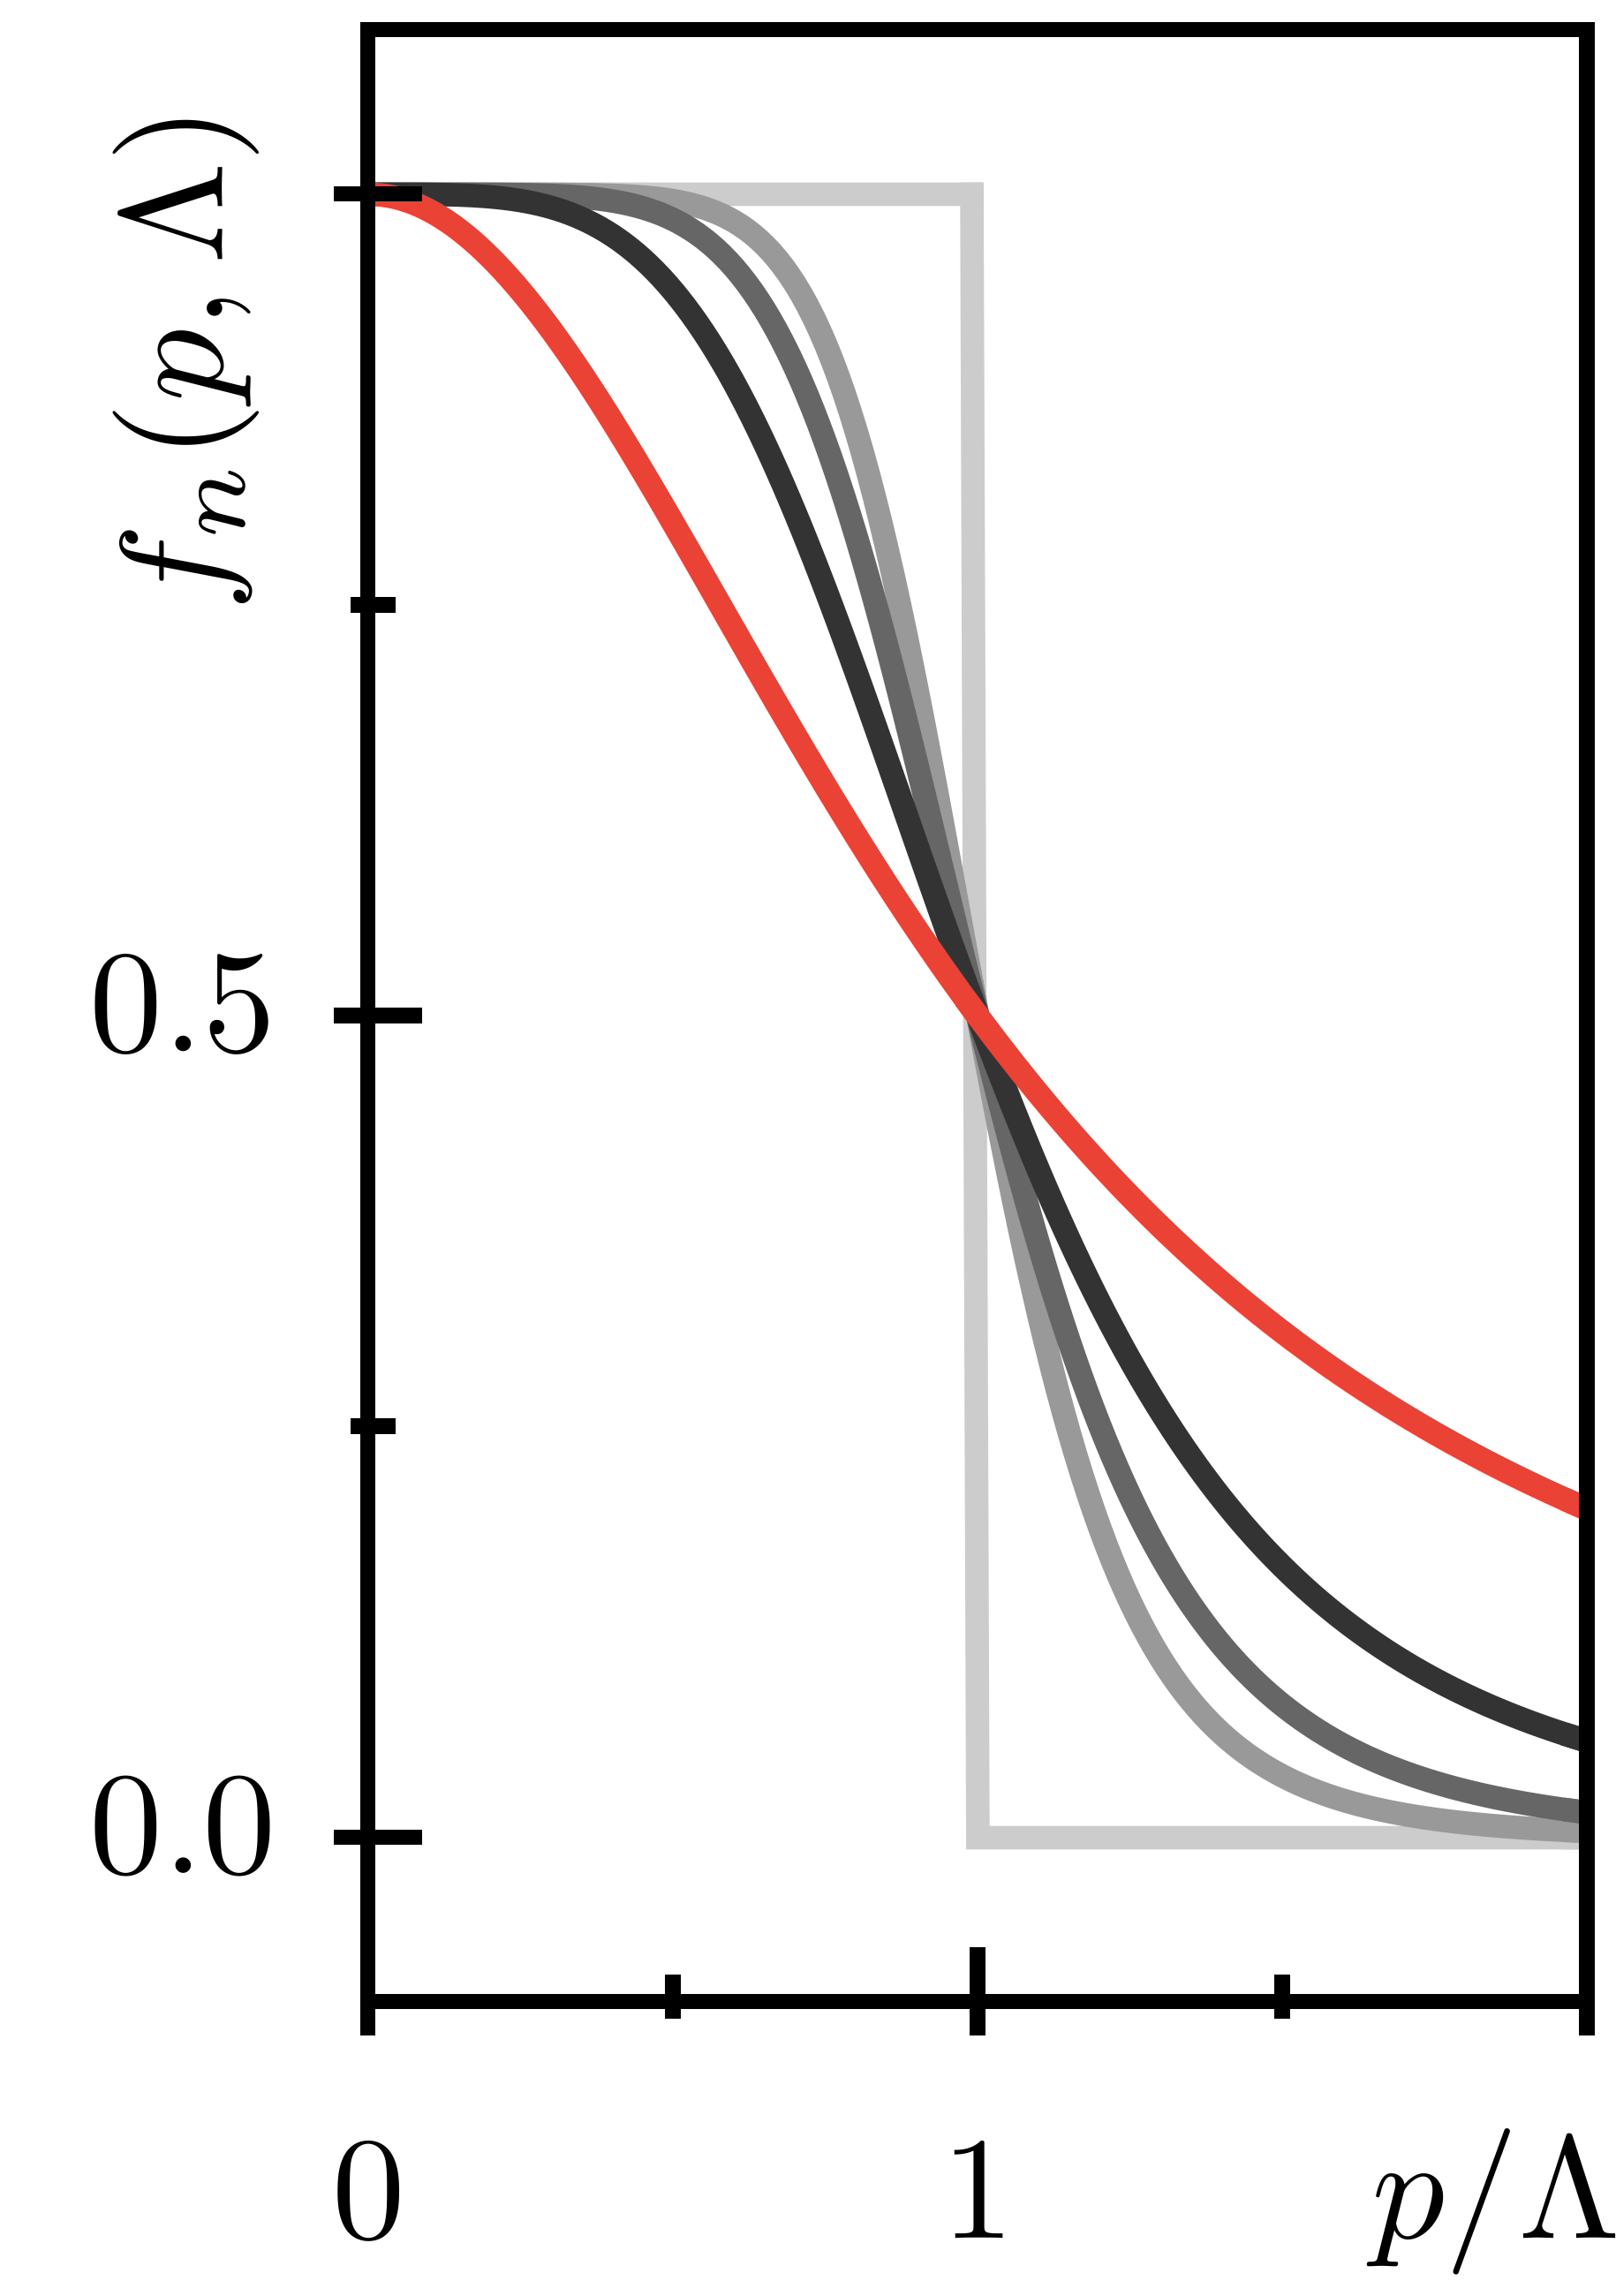
\includegraphics{figures/cutoff_function.png}}
    \subfigure[]{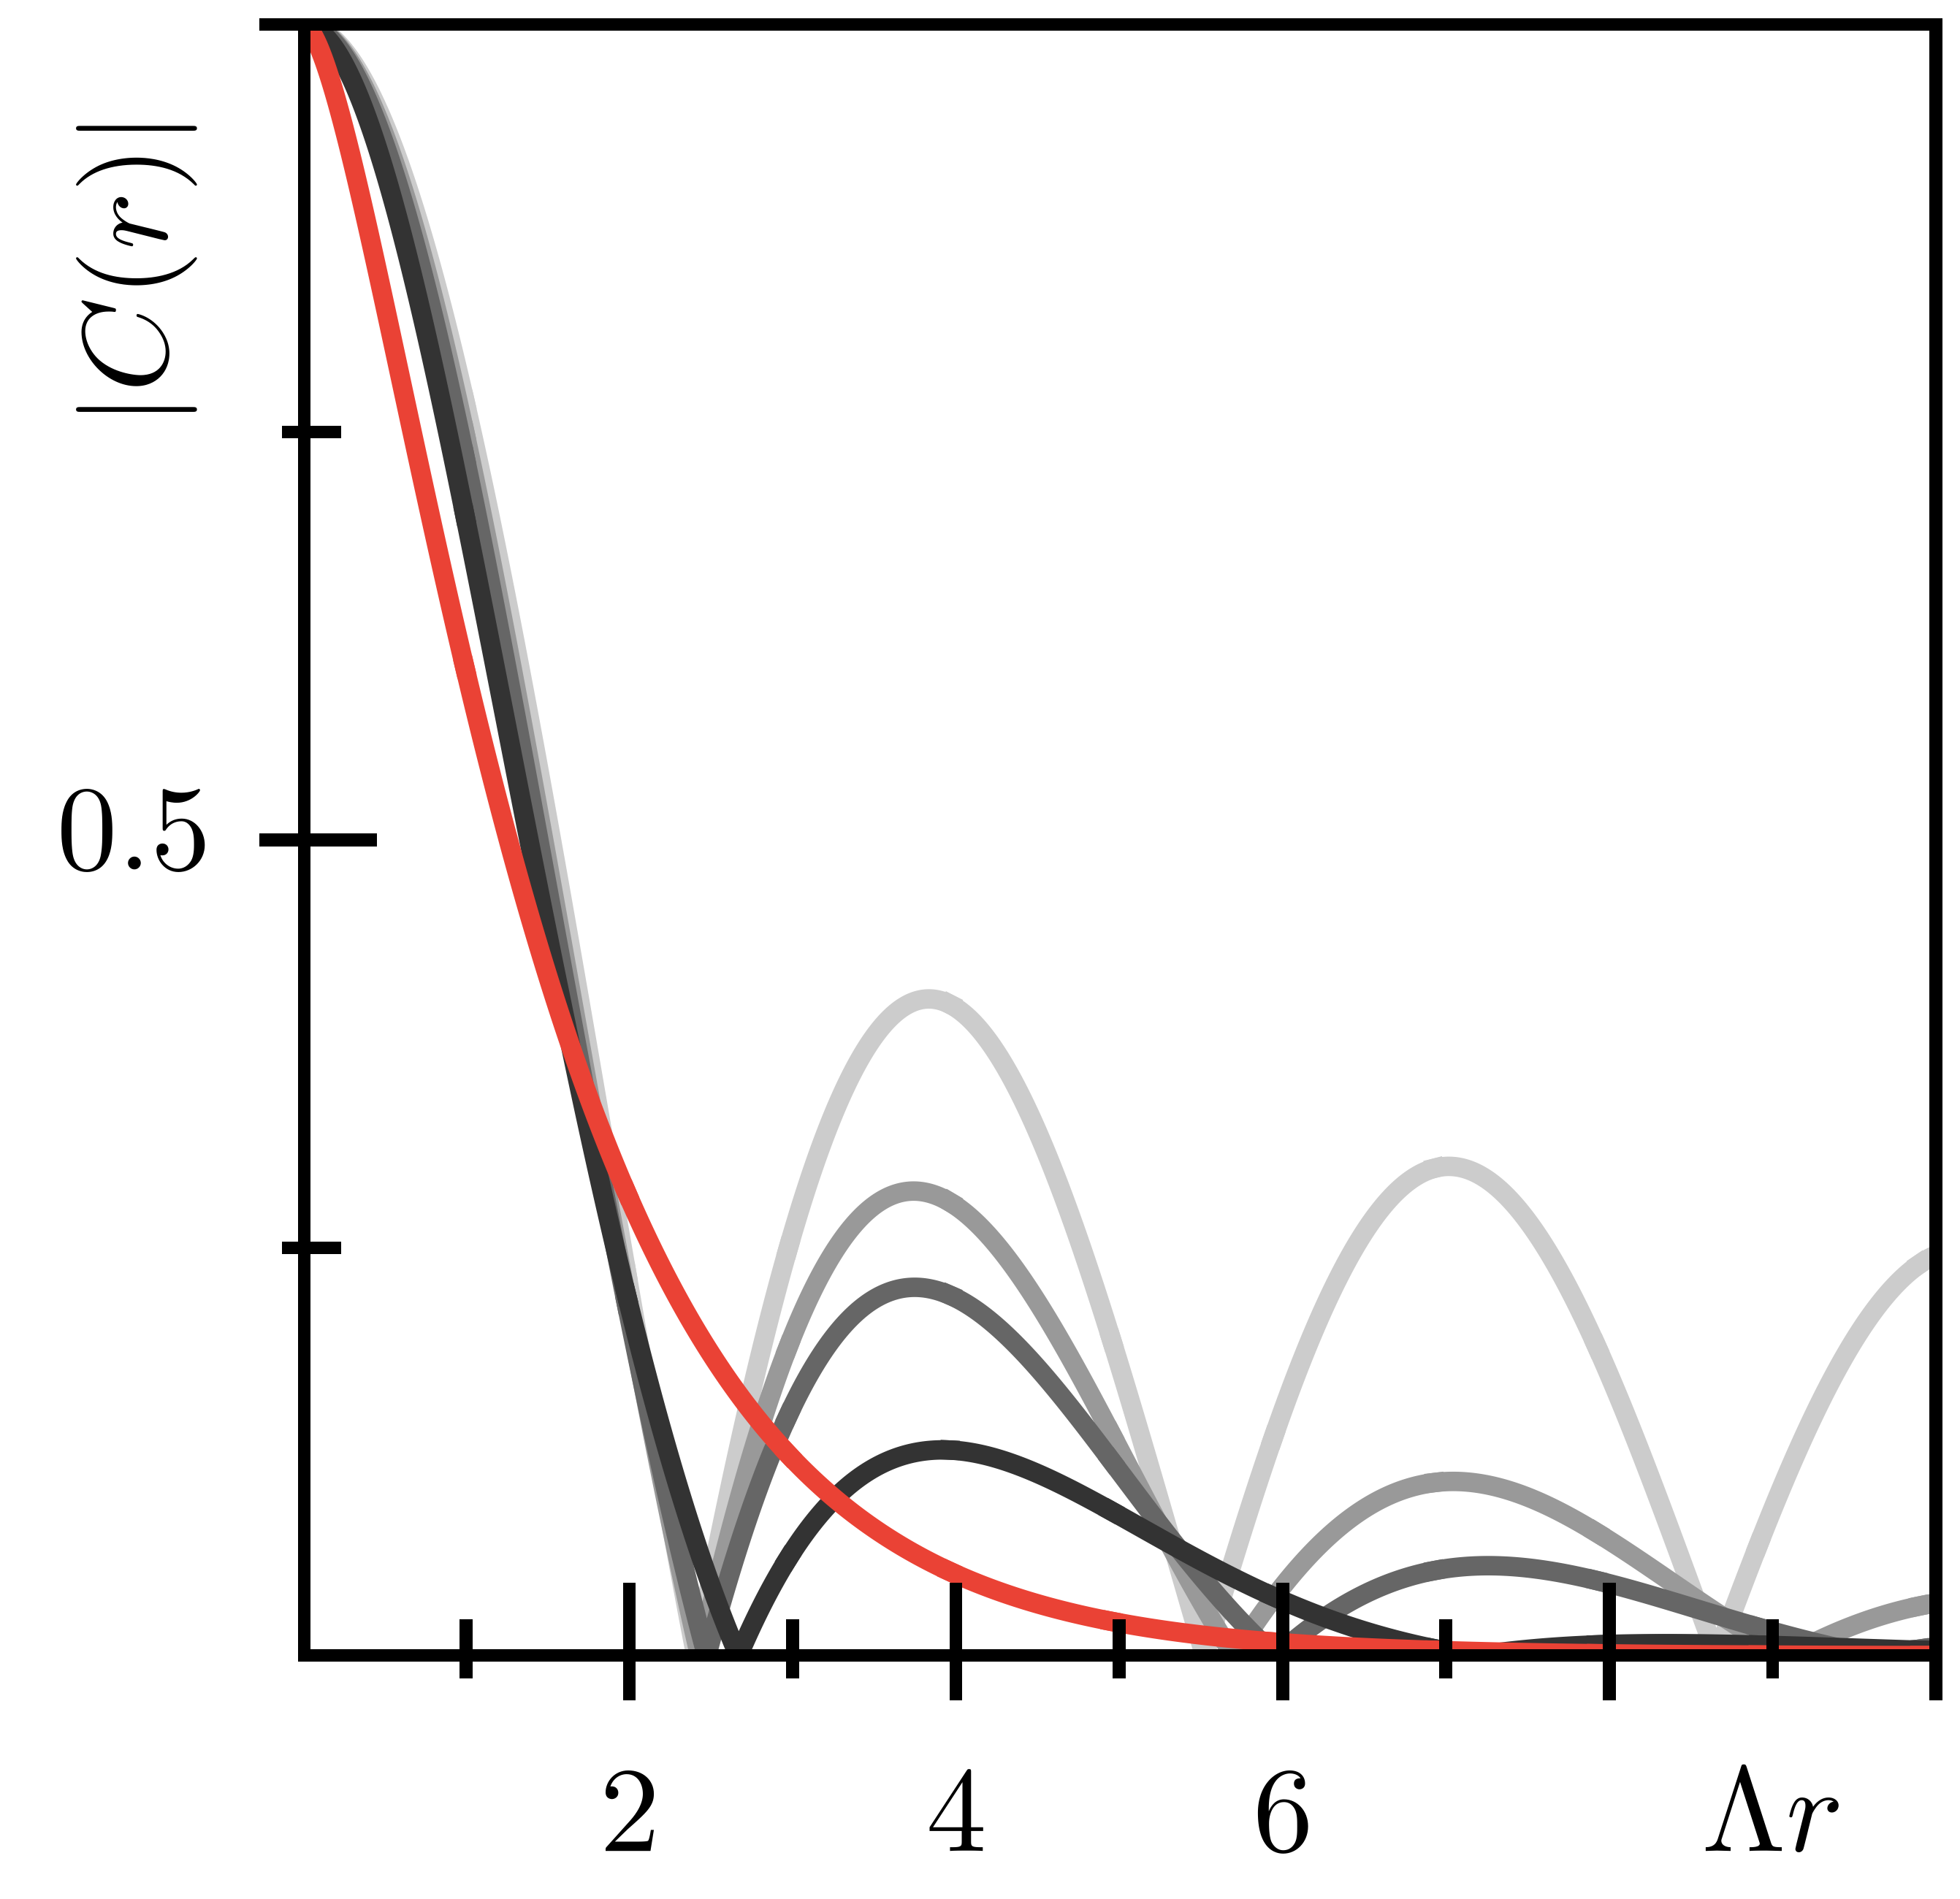
\includegraphics{figures/rg_correlations.png}}
    \subfigure[]{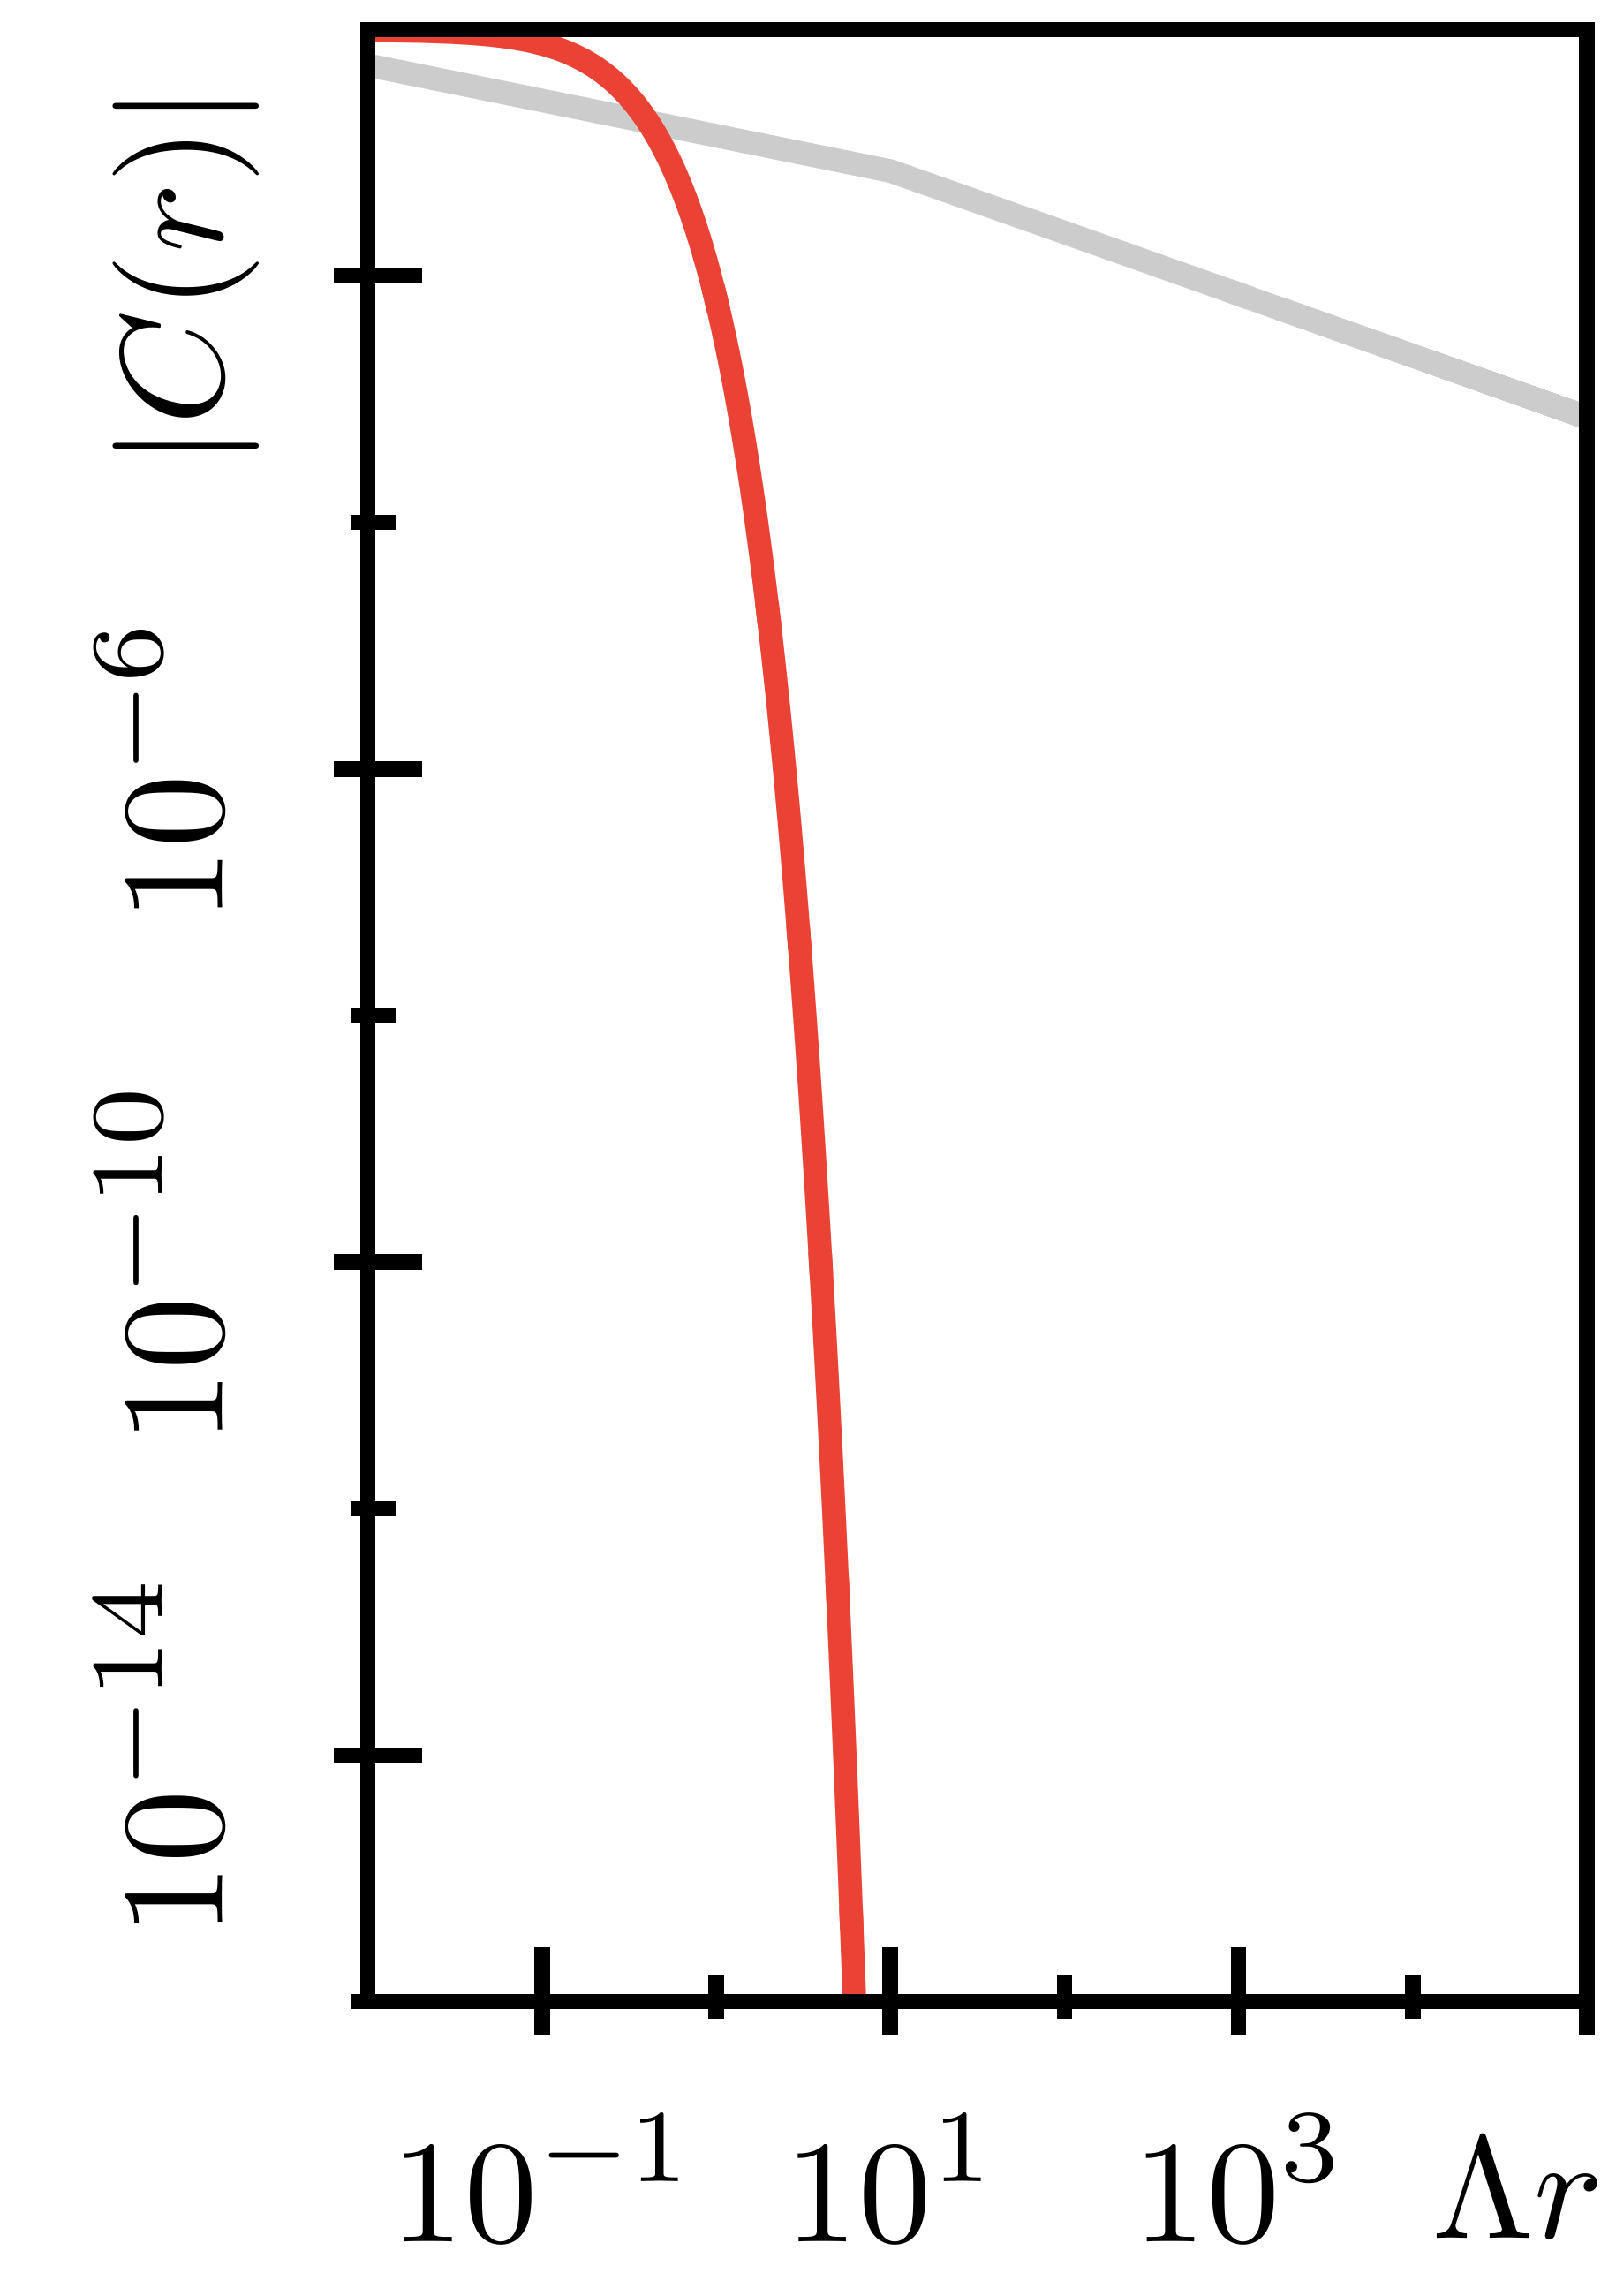
\includegraphics{figures/rg_correlations_log.png}}
    \caption{Panel (a) shows the chosen cutoff $f_n(p,\Lambda)$ with $n\in\{2,4,6,8,\infty\}$ for the integral expression in \cref{eq:integral_cutoff}, which results in various approximations of $C(r)$ for altering $n$ plotted in (b). Panel (c) highlights the exponentially sharp function $C_2(r)=\Lambda rK_1(r\Lambda)$ compared to the sharp cutoff result $C_\infty(r)=J_0(\Lambda r)$.}
    \label{fig:rg_cutoff}
\end{figure}
% At this point it is worth mentioning that the correlation functions of the slow fields are
% \begin{align}
%     \braket{\phi_\Lambda({\bm x}),\phi_\Lambda(\bm x')} = \frac K2\int_{0}^\infty\rd p J_0(p r)p^{n-1}\brlr{\frac1{p^n+\Lambda^n_{\rm min}}-\frac1{p^n+\Lambda^n_{\rm max}}}
% \end{align}
% which, in case of $n=2$, yield the appealing result
% \begin{align}
%     \braket{\phi_\Lambda({\bm x}),\phi_\Lambda(\bm x')} = \frac K2 \brlr{K_0(\Lambda_{\rm min} r) - K_0(\Lambda_{\rm max} r)}.
%     \label{eq:rg_slow_fields_approximation}
% \end{align}
For the special case $n=2$, the integral of the $h$-fields evaluates to $C_2(r)=\Lambda r K_1(\Lambda r)$ that decays exponentially fast (see \cref{fig:rg_cutoff}(c)).
In particular, the function follows the asymptotic decay $z K_1(z) \sim \sqrt{\pi z/2}\exp(-z)$ and is already negligible for $z=1$, i.e. $K_1(1)\approx0.0062$.
Therefore, the integration of $C_2(r)$ can be confined to a small interval $r<\alpha$ where $\alpha\sim2\pi/\Lambda=a$ is a small length scale comparable with the lattice spacing $a$.

In order to utilize the strong confinement of $C_2$, it is beneficial to introduce relative coordinates ${\bm R} = 1/2({\bm x}+{\bm x'})$ and ${\bm r} = {\bm x}-{\bm x'}$.
The integral can then be rewritten as
\begin{align}
    -\frac12\braket{S^2_I[\phi_{\Lambda'}+h]}_{h,{\rm conn.}}
    =
    \frac{g^2K\beta^2}8\rd l\int\rd^2R\int\rd^2r
    C_2(r)
    \left(
        \cos\commutator{\beta\phi_{\Lambda'}({\bm R}+{\bm r})+\beta\phi_{\Lambda'}({\bm R}-{\bm r})}
        \right.
        \label{eq:rg_int_1}\\
        \left.-
        \cos\commutator{\beta\phi_{\Lambda'}({\bm R}+{\bm r})-\beta\phi_{\Lambda'}({\bm R}-{\bm r})}
    \right)
    \label{eq:rg_int_2}
    \\
    \approx
    \frac{g^2K\beta^2}{8}\rd l\int\rd^2R\rd^2rC_2(r)
    \left(
        \cos\commutator{2\beta\phi_{\Lambda'}({\bm R})}
        -
        \cos\commutator{\beta\partial_{\bm R}\phi_{\Lambda'}({\bm R}){\bm r})}
    \right).
    \label{eq:rg_int_rel_coords}
\end{align}

The first $\cos$ term (\cref{eq:rg_int_1}) did not exist in the original Hamiltonian\footnote{
    Note that this term generation is continuous, and to account for it, we should start from a more generic interaction containing all the higher harmonics, i.e. $S_{I'} = S_I + \sum_{j=1}^\infty \tilde g_j\int\rd x\rd\tau\cos(2j\beta\phi)$.
    The first-order corrections of the Euclidian action then yield a coupled system of differential equations in which the amplitudes of less relevant operators depend on those of more relevant ones (but {\it not} vice-versa).
    This allows for a practical and well-justified simplification of dropping the sum in the previous expression, because the dominant coupling is always independent of the amplitudes of less-relevant operators.
} -- it is a new sine-Gordon type interaction with larger scaling dimension $D_{\tilde g} = K\beta^2$ compared to $D_g=K\beta^2/4$.
The operator associated to $\tilde g$ is thus less relevant than the original term and can be disregarded.
The second $\cos$ term in (\cref{eq:rg_int_2}) yields a renormalization of the quadratic part,
\begin{align}
    -\frac12\braket{S^2_I[\phi_{\Lambda'}+h]}_{h,{\rm conn.}}
    \approx
    \frac{\alpha^4 g^2K\beta^4}{16u^2}\rd l\int\rd x\rd\tau\frac1{u^2}(\partial_
    \tau\phi_{\Lambda'})^2+(\partial_x\phi_{\Lambda'})^2.
    \label{eq:RG_second_order_approximation}
\end{align}
In the above, I neglect a constant and gave for granted the harmonic approximation and integration of $\bm r$ with $r=\sqrt{(x-x')^2+u^2(\tau-\tau')^2}$ in polar coordinates.
The constant $\alpha^4/u^2$ is determined by the cutoff of the integrals over the relative coordinates, and $\alpha=\mathcal O(a)$ is on the order of the lattice spacing.
In summary, we obtain the effective action
\begin{align}
    S_{\rm eff}^{(2)}[\phi_\Lambda] = \frac1{2\pi}\int\rd\brlr{ x\rd\tau\frac{1}{uK'}(\partial_\tau\phi_\Lambda)^2 + \frac{u}{K'}(\partial_x\phi_\Lambda)^2} +  g'\int\rd^2 x\cos(\beta\phi_\Lambda),
\end{align}
which is self-similar to the original action up to the renormalized couplings
\begin{align}
    \frac1{uK'}=\frac1{uK}+\frac{\alpha^4 g^2 K\beta^4\pi}{8 u^4}\rd l,
    \quad
    \frac u{K'}=\frac u{K}+\frac{\alpha^4 g^2 K\beta^4\pi}{8u^2}\rd l,
    \quad
    g' = g\brlr{1 + \commutator{2-\frac{\beta^2 K}4}\rd l},
    \\
    \Rightarrow
    K' = \brlr{\commutator{\frac{1}{uK}+\frac{\alpha^4 g K\beta^4\pi}{8u^4}}\commutator{\frac{u}{K}+\frac{\alpha^4 g K\beta^4\pi}{8u^2}}}^{-1/2}
    =
    K-\frac{\pi \alpha^4 \beta^4 g^2 K^3}{8u^2}\rd l + O(\rd l^2).
\end{align}

This concludes the derivation of the so-called RG flow which is described by the system of differential equations we just derived
\begin{align}
    \frac{\rd K}{\rd l} = -\frac{\pi \alpha^4 \beta^4 g^2 K^3}{8u^2},
    \quad
    \frac{\rd g}{\rd l} = g\brlr{2-\frac{\beta^2K}4}.
\end{align}
Viable estimates are already obtained far from the phase transitions, and the second order approximation provides more insights close to the phase transition at $D_g=2$, in particular at $K=8/\beta^2$.
Equivalent results are obtained for the dual field by replacing $K\rightarrow K^{-1}$.
It is beneficial to define the flow equations close to the critical point, e.g. through the parameters
\begin{align}
    x = \frac{\beta^2 K}4 - 2,
    \quad
    y = 4g\sqrt{\frac{\pi\alpha^4}{u^2}},
\end{align}
which dictate the modified RG equations
\begin{align}
    \frac{\rd x}{\rd l} = -\frac{y^2}8(x+2)^3,
    \quad
    \frac{\rd y}{\rd l} = - xy.
\end{align}
This set of variables is particularly useful to investigate the equations in proximity of $x=0$.
Note that $(x+2)^3\approx8$, such that $\rd x/\rd l = -y^2$ and $\rd y/\rd l=-xy$ describes the effective RG flow close to the Luttinger liquid fix point at $x=0$ and $y=0$, which are known as the ``Kosterlitz-Thouless equations''~\cite{Kosterlitz1974,Kosterlitz1973}.

\begin{figure}
    \centering
    \subfigure[]{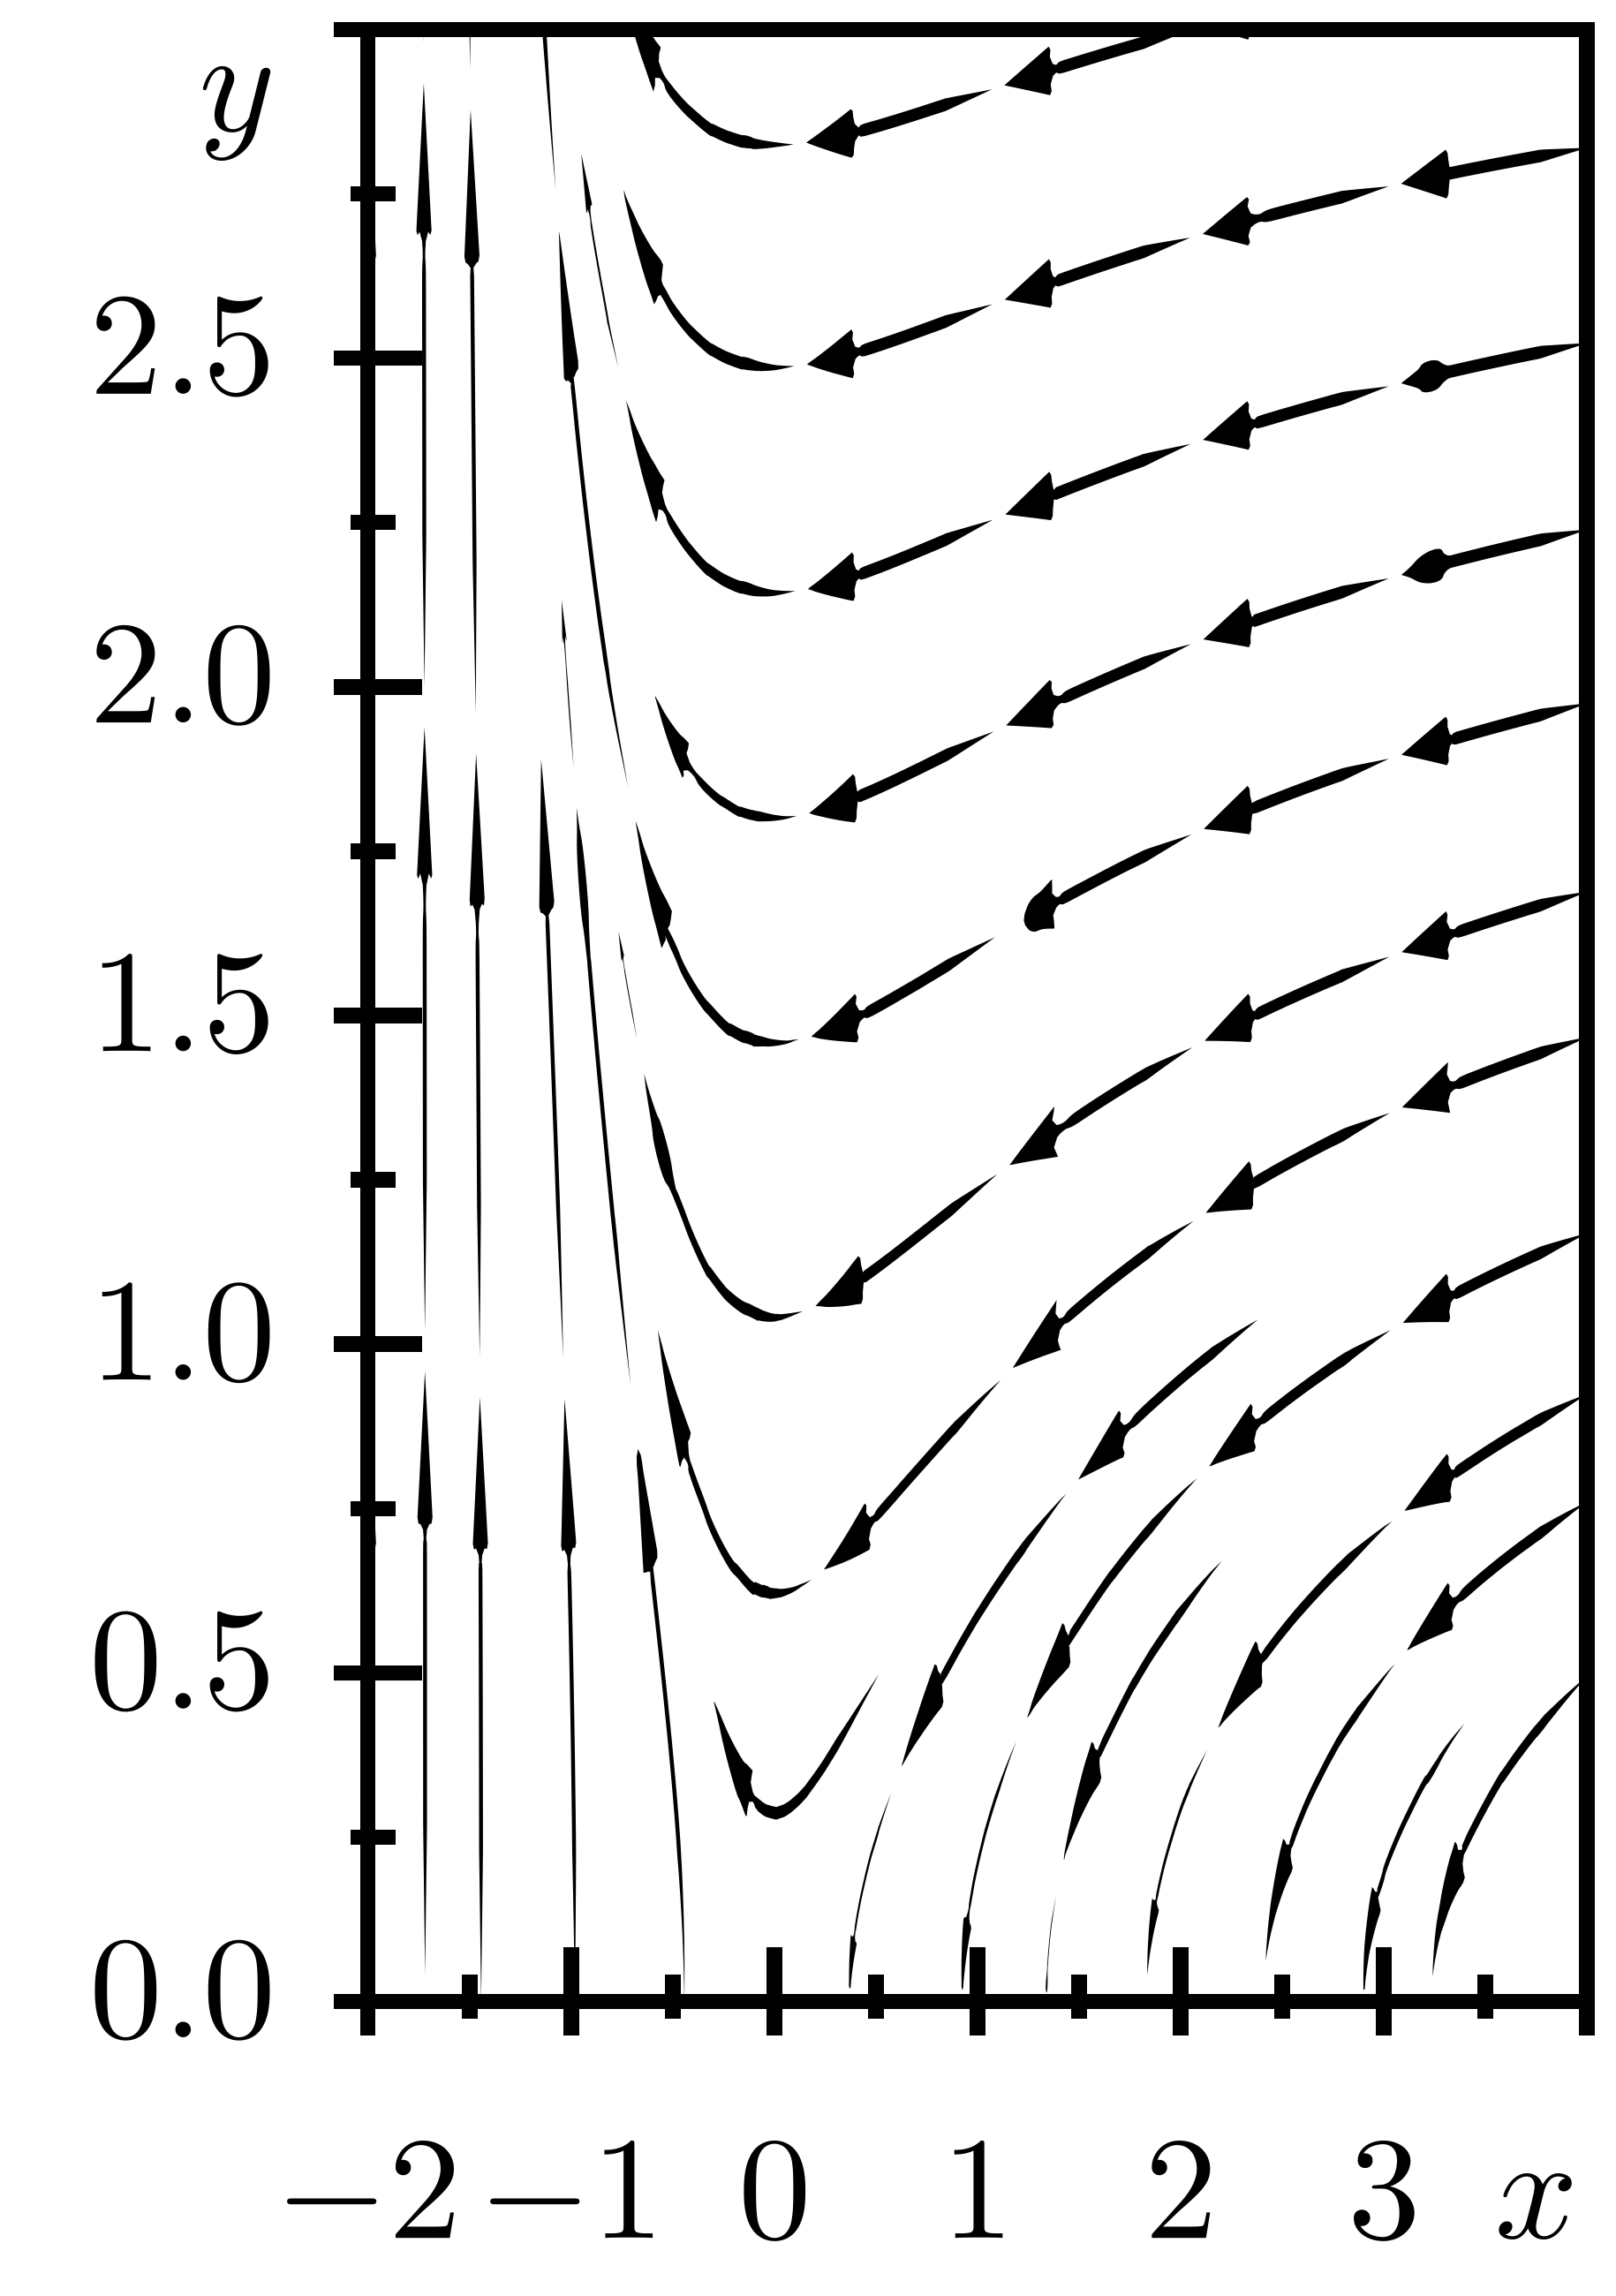
\includegraphics{figures/BKT_RG_flow1.png}}
    \subfigure[]{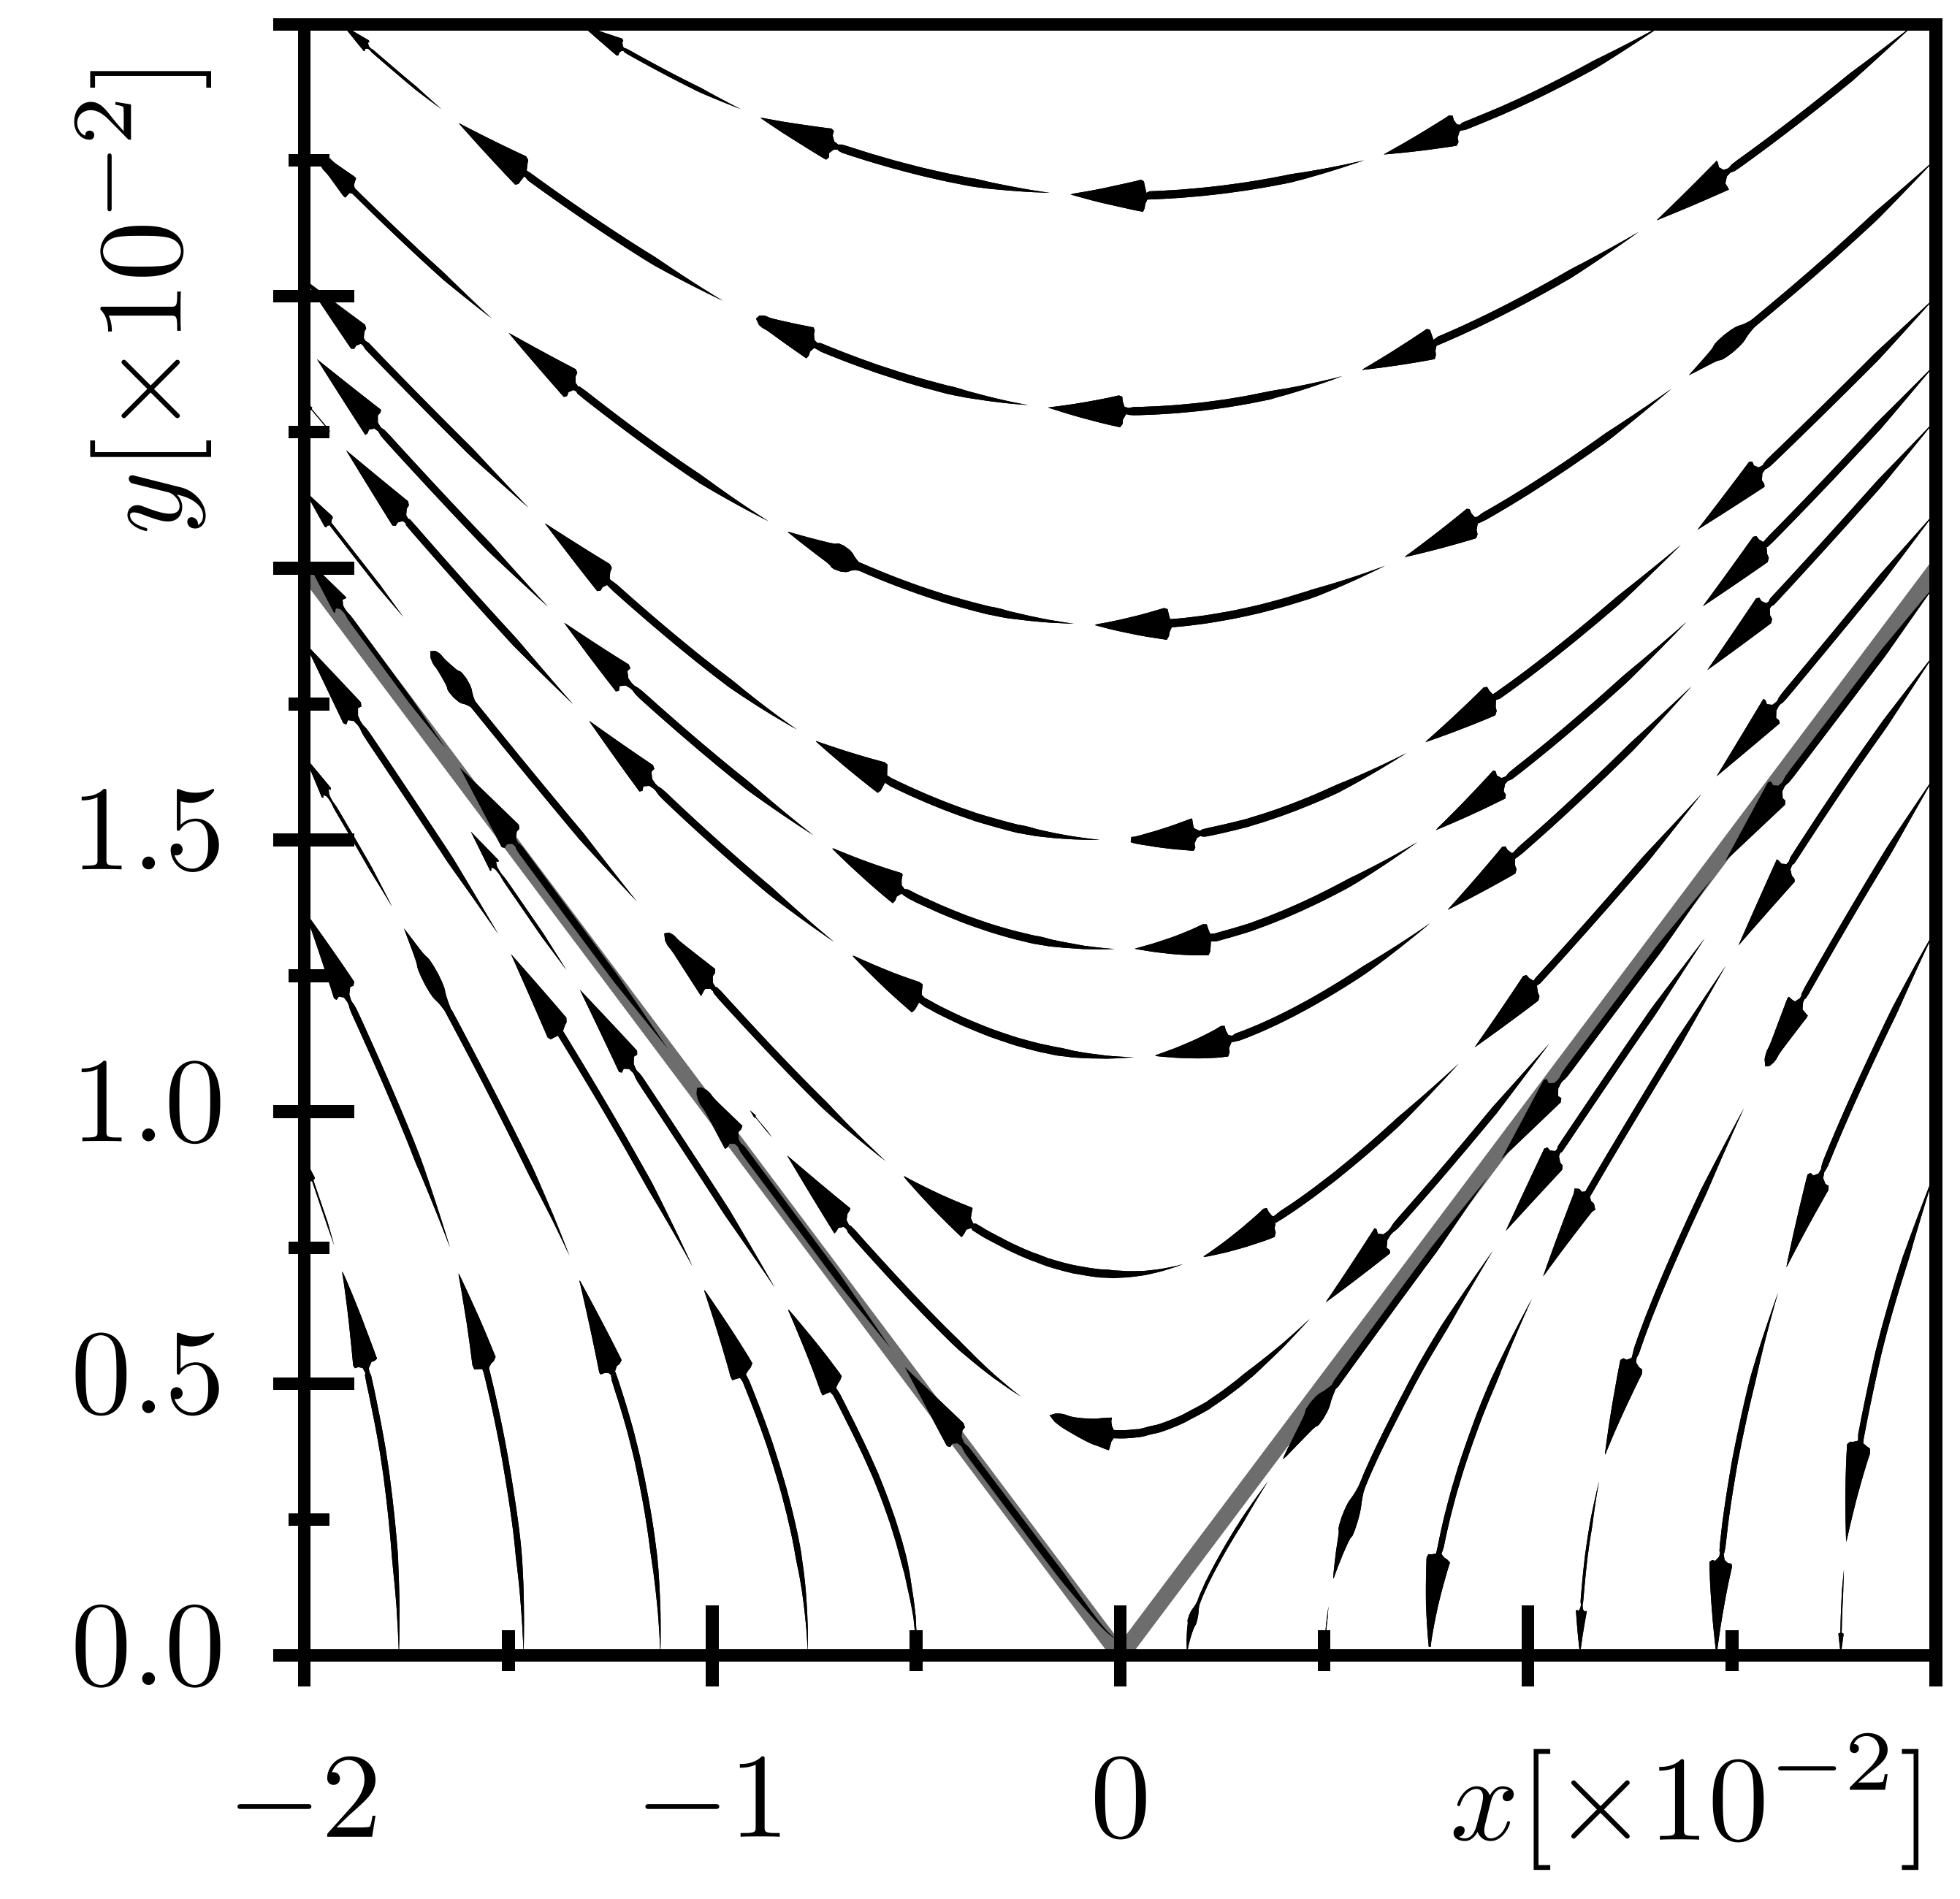
\includegraphics{figures/BKT_RG_flow2.png}}
    \subfigure[]{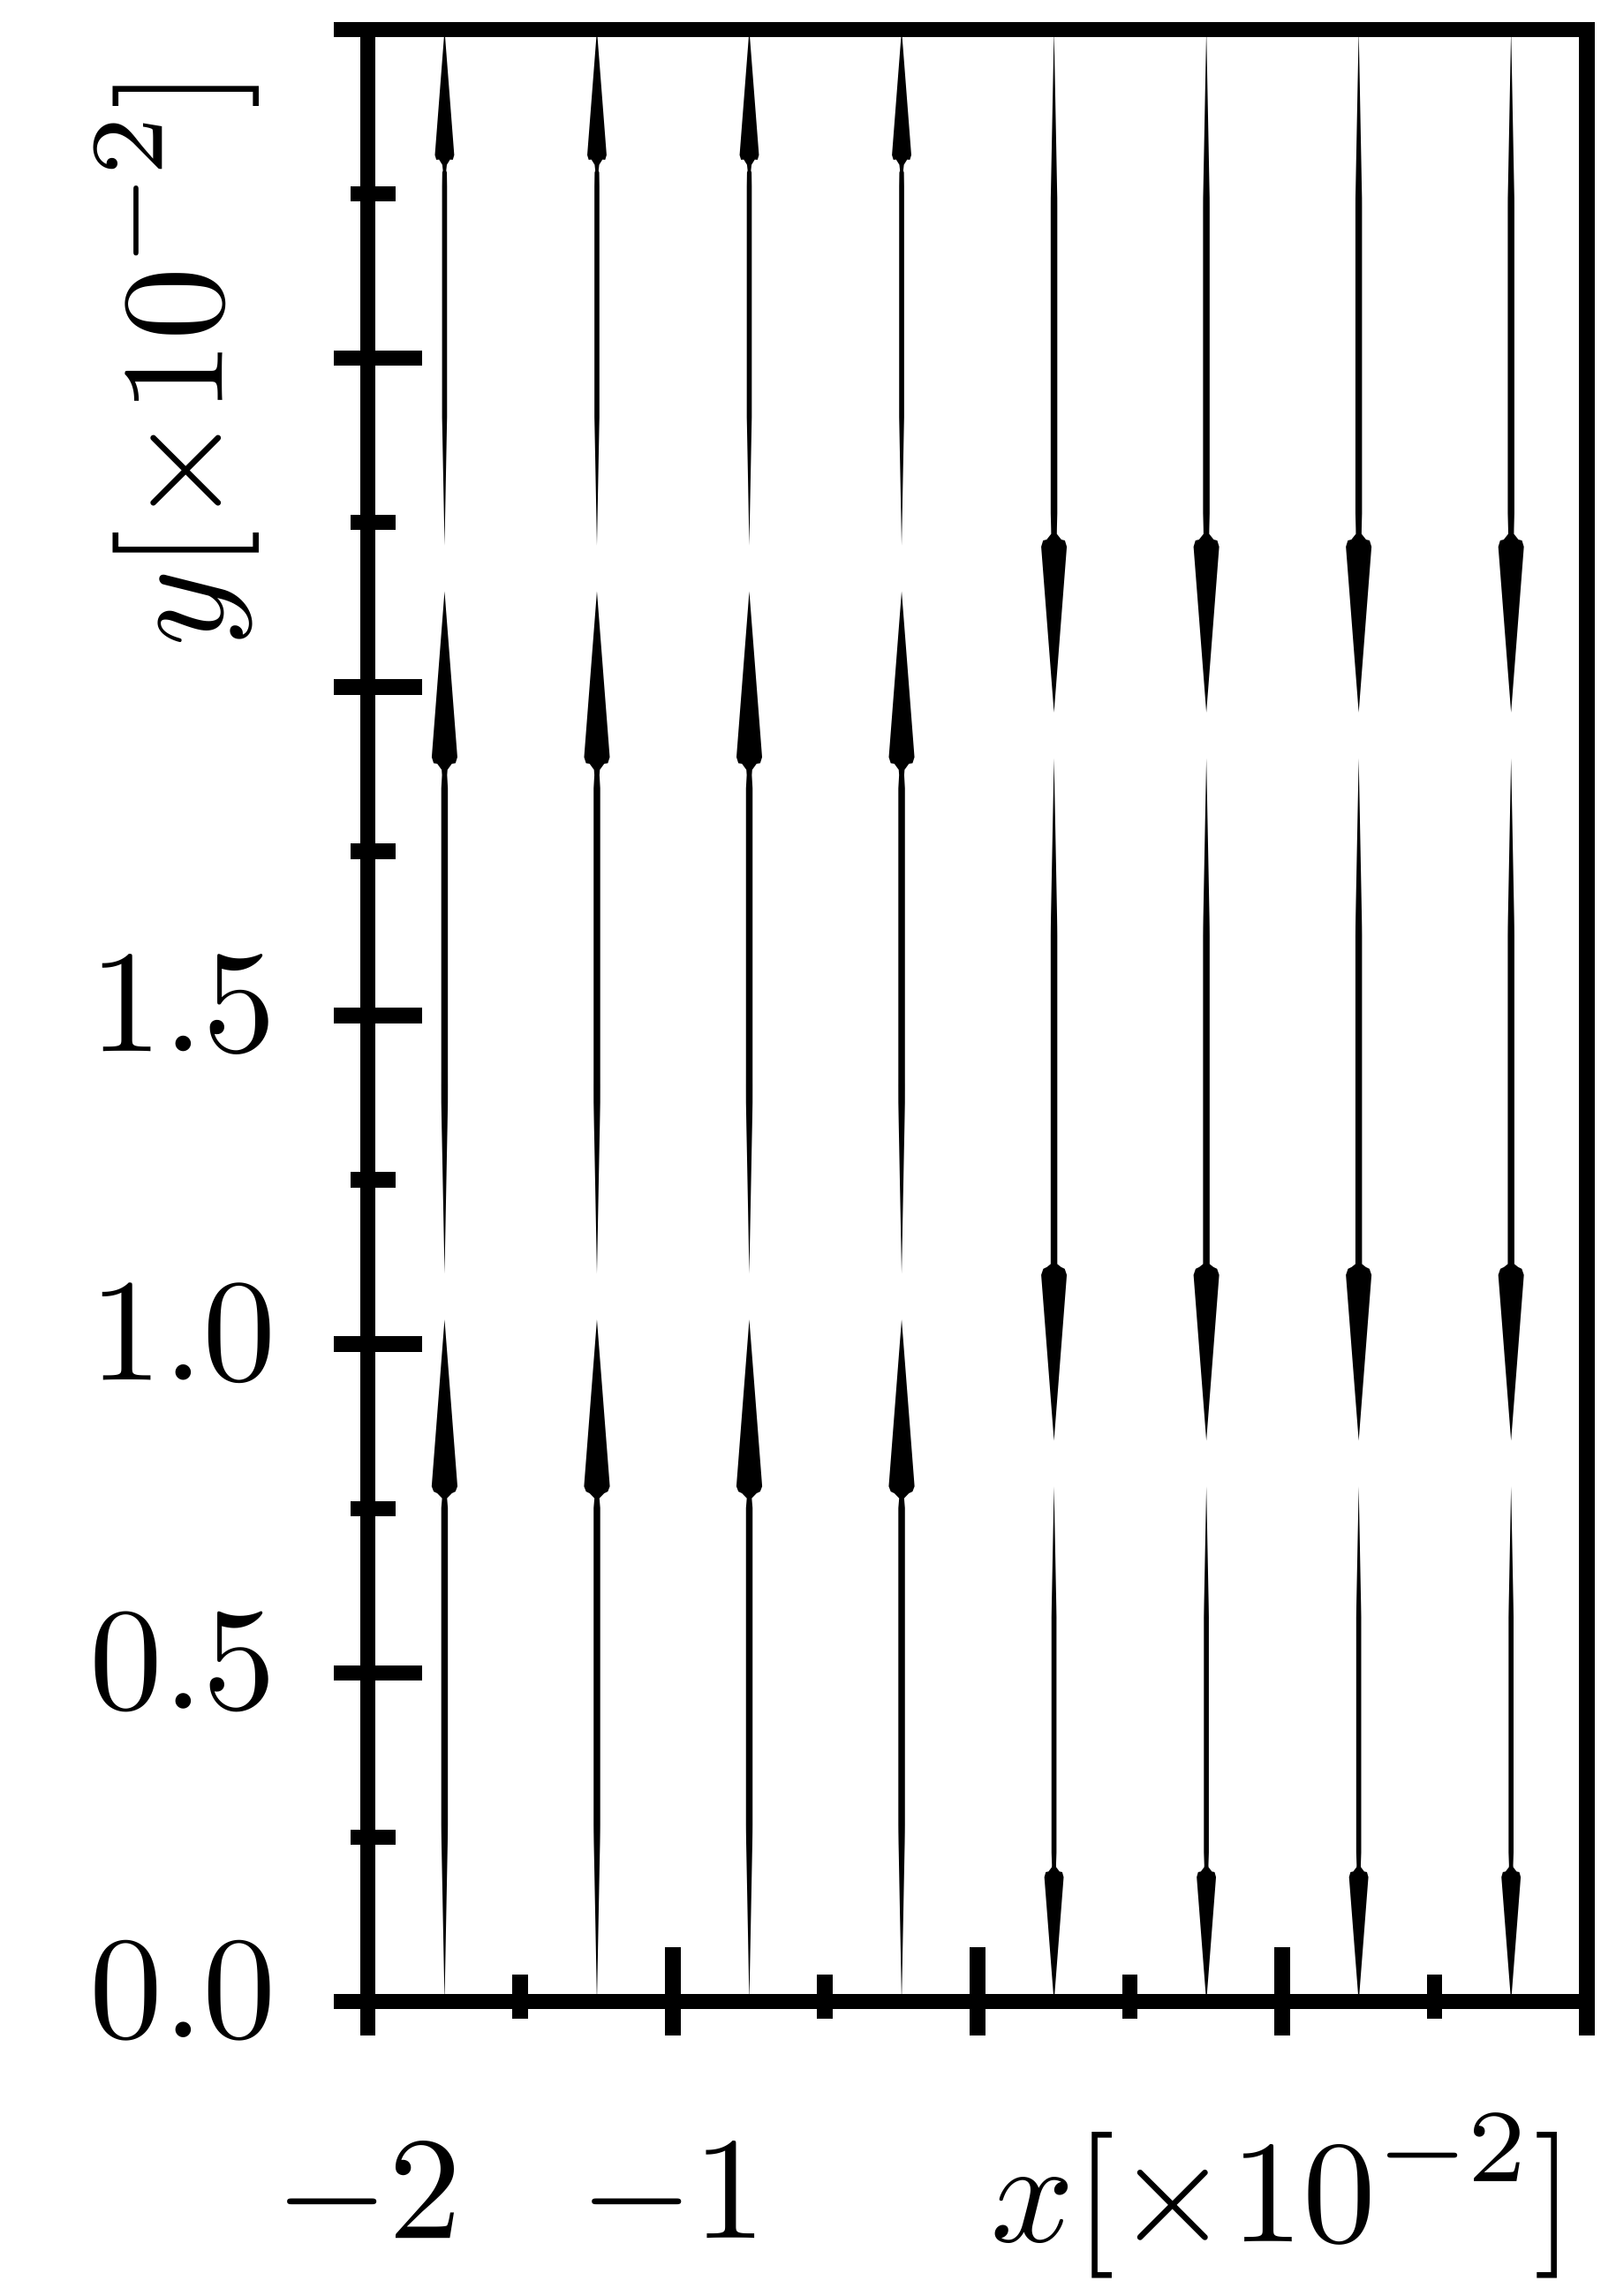
\includegraphics{figures/BKT_RG_flow3.png}}
    \caption{Plot of the modified RG equations far (a) and close (b) to the critical point $x=0$. Panel (b) close to the transition at $x=0$ shows four different scenarios for $g>0$: (i) $x>0$ and $y<x$ drives the coupling $y\rightarrow0$. This is the regime in which $g$ is irrelevant such that the system remains in the Luttinger liquid phase. (ii) $x>0$ and $y=x$ describes the critical BKT line which flows to the critical fix point $x=y=0$. (iii) $y>x$, the system always flows to $y\rightarrow\infty$ independently of $x$. (iv) $x<0$, the system flows to $y\rightarrow\infty$. Panel (c) contrasts the results of the first order RG approximation which neglects the flow of the Luttinger parameter $K$.}
    \label{fig:bkt_flow_equations}
\end{figure}

We obtain four scenarios (assuming positive couplings $y>0$ in general):

(i) If $x>0$, and $y<x$, the system flows towards $y=0$ and a finite value of $x$ at which the flow ends.
This is a situation in which the interaction is irrelevant and the coupling vanishes.
Note that a vanishing coupling $y$ implies that the flow ends, and the system thus assumes a fix point.
Although the interaction is irrelevant and as such the system remains in a Luttinger liquid phase, it ``renormalizes'' the effective Luttinger liquid parameter during the flow.
The effective interaction is then given by the final value of $x$ (thus $K$) at which the flow terminates.

(ii) If $x>0$ and $y=x$ (taken in proximity of $x$ and $y$ small), the trajectory follows a critical BKT line to the fix point $x=y=0$.
The effective Luttinger parameter assumes the ``marginal'' value $K=8/\beta^2$ for which the scaling dimension $D_g=2$.

(iii) In case of $y>|x|$, the coupling $y$ first flows towards smaller couplings, but then towards $y\rightarrow\infty$, independently on the value of $x$.
This corresponds to a case in which the interaction becomes dominating.
The Luttinger liquid description breaks down and the system ends up in a gapped phase, characterized by the interaction.

(iv) For $x<0$ and $y<|x|$, the system flows towards $y\rightarrow\infty$, which is also a gapped phase.
The dominance of $y$ is entirely determined by the initial value of $x$, and even an infinitesimal interaction amplitude results in the breakdown of the Luttinger liquid description and the formation of an energy gap.

To characterize the trajectories of the flow chart, one must notice that $x\rd x = y\rd y$ in the proximity of $x=0$, which describes the conserved quantity $c = x^2-y^2$.
The constant $c$ thus describes hyperbolas cutting the $x$ and $y$ axis for $c>0$ and $c<0$, respectively (cf. \cref{fig:bkt_flow_equations} (b)).
We focus now on the critical line $c=0, x>0$ separating relevant and irrelevant $y$.
Assume now that the microscopic Hamiltonian is described by an internal parameter $\lambda>0$ which drives the system to the BKT critical line at $\lambda_c$.
Assume further that $y$ is irrelevant for $\lambda<\lambda_c$, and relevant for $\lambda>\lambda_c$.
There are two cases:

(a) For $c>0$ and $x>0$, $y$ is irrelevant and the trajectory flows to the fix point at $x_{\rm eff} = \lim_{l\rightarrow\infty} x(l)$ and $y=0$.
We can thus linearize $c=b^2(\lambda_c-\lambda)$ in the vicinity of the critical line, in which $\lambda$ encodes an internal parameter of the microscopic Hamiltonian that drives the phase transition (see previous paragraph).
Correlations of the fields $\phi/\theta$ still decay logarithmically and the coupling is being renormalized to the asymptotic value $K_{\rm eff} = \frac4{\beta^2}\brlr{b\sqrt{\lambda_c-\lambda}+2}$, which describes a square-root singularity close to the critical point.

(b) For $c<0$ and $x>0$, $y$ is relevant and pins the field configuration to the semiclassical minima of the sine-Gordon interaction.
The differential equation can be recast to
\begin{align}
    \frac{\rd x}{\rd l} = -y^2 = c-x^2 = -(|c|+x^2)
    \Rightarrow
    \int_{x(0)}^{x(l)}\rd x(x^2+|c|)^{-1} = -l
    .
\end{align}
The solution is thus given by $x(l) = \sqrt{|c|}\tan(\arctan(x(0)/\sqrt{|c|})-l\sqrt{|c|})$ and the integration must be terminated when $|x(l^*)|\sim 1$ (for which the perturbative calculation is invalid), i.e.
\begin{align}
    l^*=\frac{\pi}{2\sqrt{|c|}}+\frac{\arctan\brlr{\frac{x(0)}{\sqrt{|c|}}}}{\sqrt{|c|}}\approx \frac{\pi}{2b\sqrt{\lambda-\lambda_c}}.
\end{align}
An estimate of the correlation length in the system after the RG flow is given by \cref{eq:correlation_length_rg_flow}, and evaluates to $\xi\propto a\exp(l^*)=a\exp[{{\pi}/({2b\sqrt{\lambda-\lambda_c}})}]$.
Any attempt to realize systems close to the phase transition thus requires system lengths in excess of the exponentially divergent correlation length.
The requirement for numerical techniques is thus two-fold: resolving the phase transition requires excessively long systems, and must capture a divergent correlation length.
One simulation technique which was successfully applied for such tough systems is the density matrix renormalization group (DMRG) based on matrix product states (MPS), which I formalize in \cref{ch:matrix_product_states}.
This is to say that the bottleneck of MPS to be efficient is based on simulating systems with a short correlation length (see \cref{sec:scaling_relations_of_the_entanglement_entropy}).
However, pushing the limits of state-of-the-art MPS algorithms and CPU's overcomes the related issues and allows to extract quantitative results with great success, even if the correlation length is large.

In \cref{one_half1,integer1}, we encounter various types of sine-Gordon terms embedded in a two-component Luttinger liquid.
Among those which are potentially relevant, we characterize the phase diagram by a second order RG analysis equivalent to the example detailed in this section.
In general, the resulting RG equations are not the simple two-variable BKT equations and they form a higher dimensional flow chart.
We thus rely on numerical integration of coupled differential equations through Runge-Kutta methods to determine the relevancy of operators.
For more quantitative estimates, we use MPS simulations.

%!TEX root = thesis.tex
%%%%%%%%%%%%%%%%%%%%%
%
%
%%%%%%%%%%%%%%%%%%%%%%%%%%%%%%%%%
%%%%%%%%%%%%%%%%%%%%%%%%%%%%%%%%%
\chapter{Matrix product states}
\label{sec:matrix_product_states}
%%%%%%%%%%%%%%%%%%%%%%%%%%%%%%%%%
%%%%%%%%%%%%%%%%%%%%%%%%%%%%%%%%%
The analytical treatment as presented in the previous chapter relies on a heavy line of approximations (which are sometimes very hard to justify on a rigorous level).
One of the most crucial consequences is that quantitative deviations occur if the interactions are comparable to the kinetic bandwidth.
This restricts heavily the validity region of the low-energy effective field theory of a particular model.
To make an example, a sine-Gordon term with $\beta=4$ is encountered in the effective low-energy field theory of the spin-$1/2$ XXZ chain and the interaction will be relevant in the RG sense for $K<1/2$.
However, such a small Luttinger parameter requires very strong nearest neighbor interactions in real systems that are compatible with the system's bandwidth, which thus implicitly breaks the assumptions to derive the effective low-energy field theory itself.
Although the field theoretic description might not break down entirely, heavy quantitative deviations from the Luttinger liquid predictions of the effective coupling parameters are to be expected.
This motivates the use of numerical tools to verify the analytic predictions in the strongly interacting cases.
In this chapter, I will provide the essentials to get acquainted with the concepts of tensor networks, in particular with matrix product states (MPS).
\\

First, I give a basic introduction to tensor networks and explain the intuitive concept of renormalization through a truncation of the auxiliary dimension of these structures.
Second, I review the concept of ``area laws'' -- a statement about the structure of quantum correlations of gapped and short-ranged Hamiltonians -- and connect it to the properties of tensor networks.
I will then present renormalization strategies which provide variational search algorithms to target ground (and low-lying excited) states and continue by presenting a simple yet effective time-evolution algorithm in the framework of MPS.
As a conclusion, I review the exploit of abelian symmetries in the numerical techniques which in general reduces the overall computational complexity.
%
%
%%%%%%%%%%%%%%%%%%%%%%%%%%%
\section{Tensor networks}
\label{sec:tensor_networks}
%%%%%%%%%%%%%%%%%%%%%%%%%%%
A tensor is a collection of complex numbers in multidimensional arrays.
Its rank is given by the number of indices: for instance, scalar values are of rank zero, vectors of rank one and matrices of rank two.
Tensor networks are in general contractions of many tensors and as such it is customary to define graphical representations which display its fundamental structure, i.e. its rank.
The most common convention is to represent a tensor object as a circle, triangle, hourglass or rectangle with as many legs as the tensor has indices.
It is then easy to sketch the tensor contraction of a simple matrix-matrix multiplication as
\begin{align}
    C_{i,j}=A_{ik}B_{kj}\equiv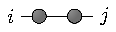
\includegraphics[valign=c]{figures/MatrixMultiplication.pdf},
\end{align}
in which I conveniently use the sum convention.
Switching from formulas to graphical notation may become interesting when considering larger tensor networks.
One easy example is a trace of many matrices, which can be sketched as a circle contraction.
\begin{align}
    \tr\brlr{ABCDEF} \equiv 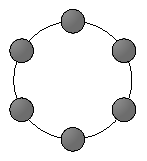
\includegraphics[valign=c]{figures/MatrixTrace.pdf}.
\end{align}
For more complex contractions containing tensors of higher ranks, it is important to optimize the sequence of contractions to reduce the overall computational cost to a minimum.
For instance, in \cref{fig:contraction_sequences} two different sequences of contractions obviously result in the same outcome, but the overall complexity class is different.
Assume each leg has dimension $m$, then sequence $S_1$ is $O(m^4)$ whereas sequence $S_2$ is $O(m^4)$.
\begin{figure}
    \centering
    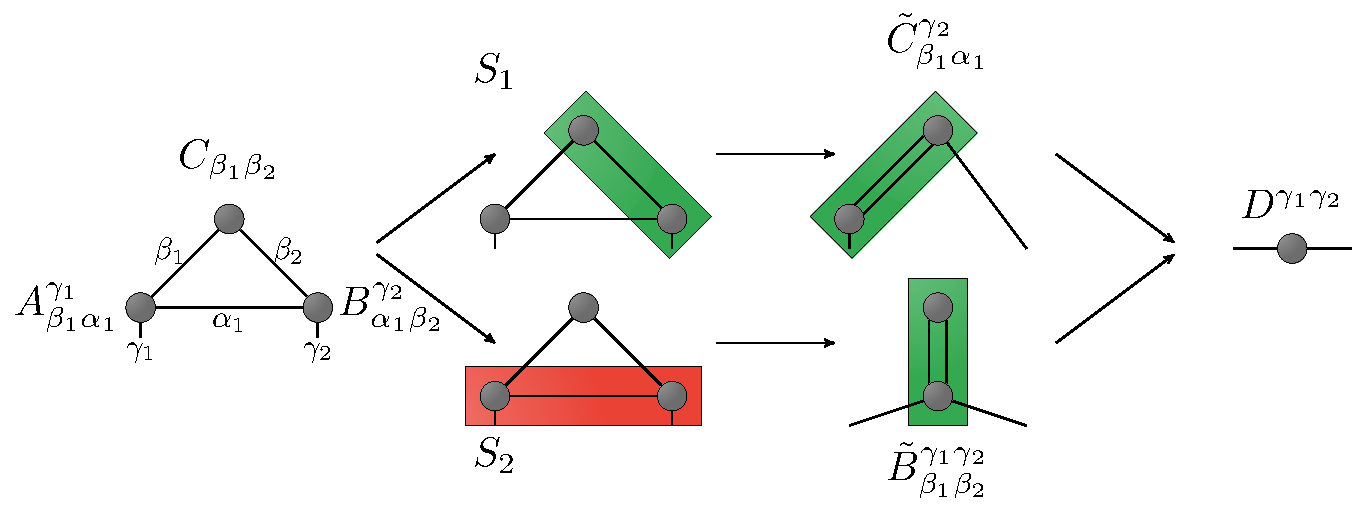
\includegraphics[width=0.8\textwidth]{figures/ComplexContraction1.pdf}
    \caption{Different complexity classes for the same contraction, but different sequences. Assume each index has dimension $m$, then the green contractions are $O(m^4)$, but red is $O(m^5)$. Hence, sequence $1$ requires less multiplications compared to $2$ and is thus less prone to numerical truncation errors.}
    \label{fig:contraction_sequences}
\end{figure}
A triangle representation may make sense to indicate a tensor being an isometry.
For instance, consider the two isometries $U$, $V^\dag$ of a generic singular value decomposition (SVD) $M = U \Lambda V^\dag$: they contain the left- and right-singular vectors of $M$ and are thus semi-unitaries, i.e.
\begin{align}
    U^\dag U^\pdag = \mathbb1,
    \quad
    V^\dag V^\pdag = \mathbb1.
\end{align}
In graphical notation, the identity matrix is represented as a straight line as it does neither stretch nor rotate the entries of a tensor.
The previous equation can thus be recast to
\begin{align}
    U^\dag U^\pdag \equiv 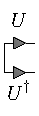
\includegraphics[valign=c]{figures/right_isometry.pdf} = 
\includegraphics[valign=c]{figures/right_identity.pdf}\,,
    \qquad
    V^\dag V^\pdag \equiv 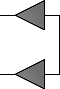
\includegraphics[valign=c]{figures/left_isometry.pdf} = 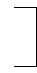
\includegraphics[valign=c]{figures/left_identity.pdf}\,.
    \label{eq:isometries}
\end{align}
A simple squared unitary matrix is orthogonal with respect to both left/right multiplication with its adjoint and as such can be represented as a hourglass.
The SVD of a normal matrix $M$ can be recast to the graphical notation
\begin{align}
    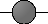
\includegraphics[valign=c]{figures/matrix.pdf}
    \equiv M = U \Lambda V^\dag \equiv
    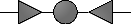
\includegraphics[valign=c]{figures/svd.pdf}\,.
\end{align}
Let me now introduce probably the most important decomposition applied in tensor networks -- the generalized version of the SVD for rank $n$ tensors:
(i) the rank $n$ array has to be reduced to a rank $2$ object, i.e. a matrix.
This transformation (which must be a bijection) is commonly called tensor reshaping and is understood in graphical notation as a fusion of multiple tensor legs.
(ii) The matrix then is decomposed through a standard SVD, followed by (iii) the restoration of the original rank $n$ object through the inverse reshaping applied in step (i).
The identity relation between the original and decomposed tensor is assured by the inverse of (i).
For a practical example, consider a rank $n$ tensor $T$ which is graphically depicted by $n$ legs (labelled by increasing numbers from $1,...,n$ from left to right).
To perform a SVD between the bipartition after leg $j$, the tensor is reshaped to a matrix through a fusion of legs $1,...,j$ and $j+1,...,n$ prior to the performed SVD, after which the original rank is restored.
In particular, the sequence of identities reads
% \begin{align}
%     % 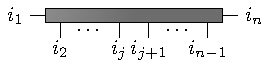
\includegraphics[valign=c]{figures/rankntensor.pdf}
%     % =
%     T_{i_1,i_n}^{i_2,\dots,i_j,i_{j+1},\dots,i_{n-1}}
%     &\overset{(i)}{=}
%     f^{-1}\circ T_{(i_1,\dots,i_j),(i_{j+1},\dots,i_n)}
%     \\
%     &\overset{(ii)}{=}
%     f^{-1}\circ\sum_k U^\pdag_{(i_1,\dots,i_j),k}S^\pdag_{k}{V^\dag}_{k,(i_{j+1},\dots,i_n)}
%     \\
%     &\overset{(iii)}{=}
%     \sum_kU_{i_1,k}^{i_2,\dots,i_j}S^\pdag_{k}{V^\dag}_{k,i_n}^{i_{j+1},\dots,i_{n-1}},
% \end{align}
\begin{align}
    T_{i_1,i_n}^{i_2,\dots,i_j,i_{j+1},\dots,i_{n-1}}
    \equiv&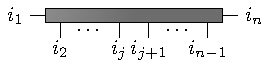
\includegraphics[valign=c]{figures/rankntensor.pdf},
    \\
    \overset{(i)}{=}&
    f^{-1}\circ
    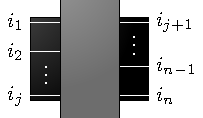
\includegraphics[valign=c]{figures/reshaping.pdf}
    \equiv
    f^{-1}\circ U^\pdag_{(i_1,\dots,i_j),k}\Lambda^\pdag_{k}V^\dag_{k,(i_{j+1},\dots,i_n)},
    \\
    \overset{(ii)}{=}&
    f^{-1}\circ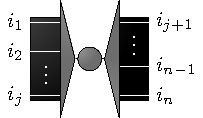
\includegraphics[valign=c]{figures/bigsvd.pdf}
    \equiv
    f^{-1}\circ U^\pdag_{(i_1,\dots,i_j),k}\Lambda^\pdag_{k}V^\dag_{k,(i_{j+1},\dots,i_n)},
    \\
    \overset{(iii)}{=}&
    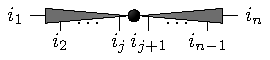
\includegraphics[valign=c]{figures/rankntensor_decomposed.pdf}
    \equiv
    U_{i_1,k}^{\pdag i_2,\dots,i_j}\Lambda^\pdag_{k}{V^\dag}^{i_{j+1},\dots,i_{n-1}}_{k,i_n},
    \label{eq:SVD_generalized}
\end{align}
in which $f^{-1}$ denotes the inverse of the tensor reshaping / leg fusion, and Einstein notation implies the tensor contraction contraction with summed index $k$.
In the equations above, it is assumed that the applied SVD is compact: $\Lambda$ is a square and diagonal matrix containing the nonzero singular values, such that $\Lambda_{ij}\equiv s_i\delta_{ij}$.
\\

To get acquainted with the use of tensors in a more practical sense, let us aim to understand some of the described concepts in the context of two-dimensional pictures.
If we assume the picture to be rasterized in an equidistant manner using square pixels, the RGB-entries of the pixel can be collected in a 3D array of the form
\begin{align}
    P_{y,x}^{c}\equiv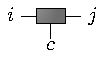
\includegraphics[valign=c]{figures/tensor_picture.pdf}.
\end{align}
The position of the pixel is encoded by the indices $y,x$ and $c$ represents a leg containing the RGB-values (e.g., $c\in\{1,2,3\}\equiv\{r,g,b\}$).
Using the concept of the generalized SVD, we can decompose the tensor $P$ into two semi-unitaries $U,V^\dag$ and a vector $S_k$ containing the singular values of the bipartition.
There exist three different bipartitions: (a) $P_{(y,x),c}$, (b) $P_{(y,c),x}$ and (c) $P_{y,(x,c)}$.
(b) and (c) are equivalent up to a transposition of the original object, therefore leaving two truly different decompositions, (a) and (b).
The bipartition (a) targets a decomposition between $(y,x)$ and $c$ whereas (b) targets a decomposition between $y$ and $(x,c)$.
Strategy (a) thus aims to truncate the color degree of freedom, which is not very useful due to the low dimensionality of the $c$ leg (there are only $3$ nonzero singular values to begin with), such that I will focus entirely on the decomposition of (b).
\\

\begin{figure}
    \centering
    \subfigure[]{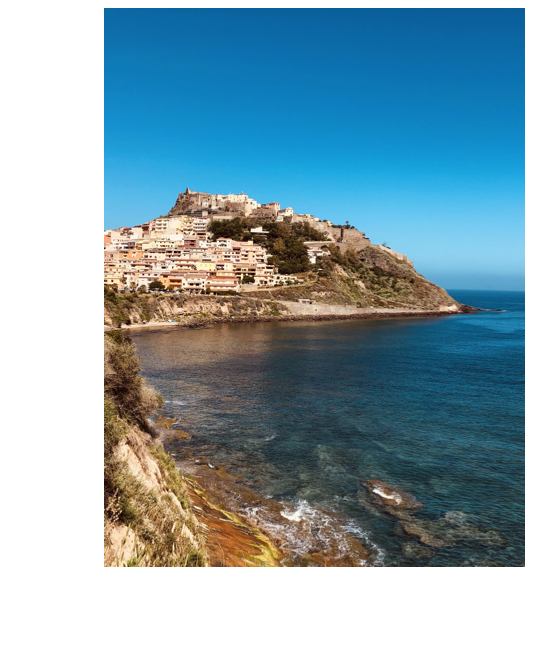
\includegraphics{figures/SVD_uncompressed.png}}
    \hfil
    \subfigure[]{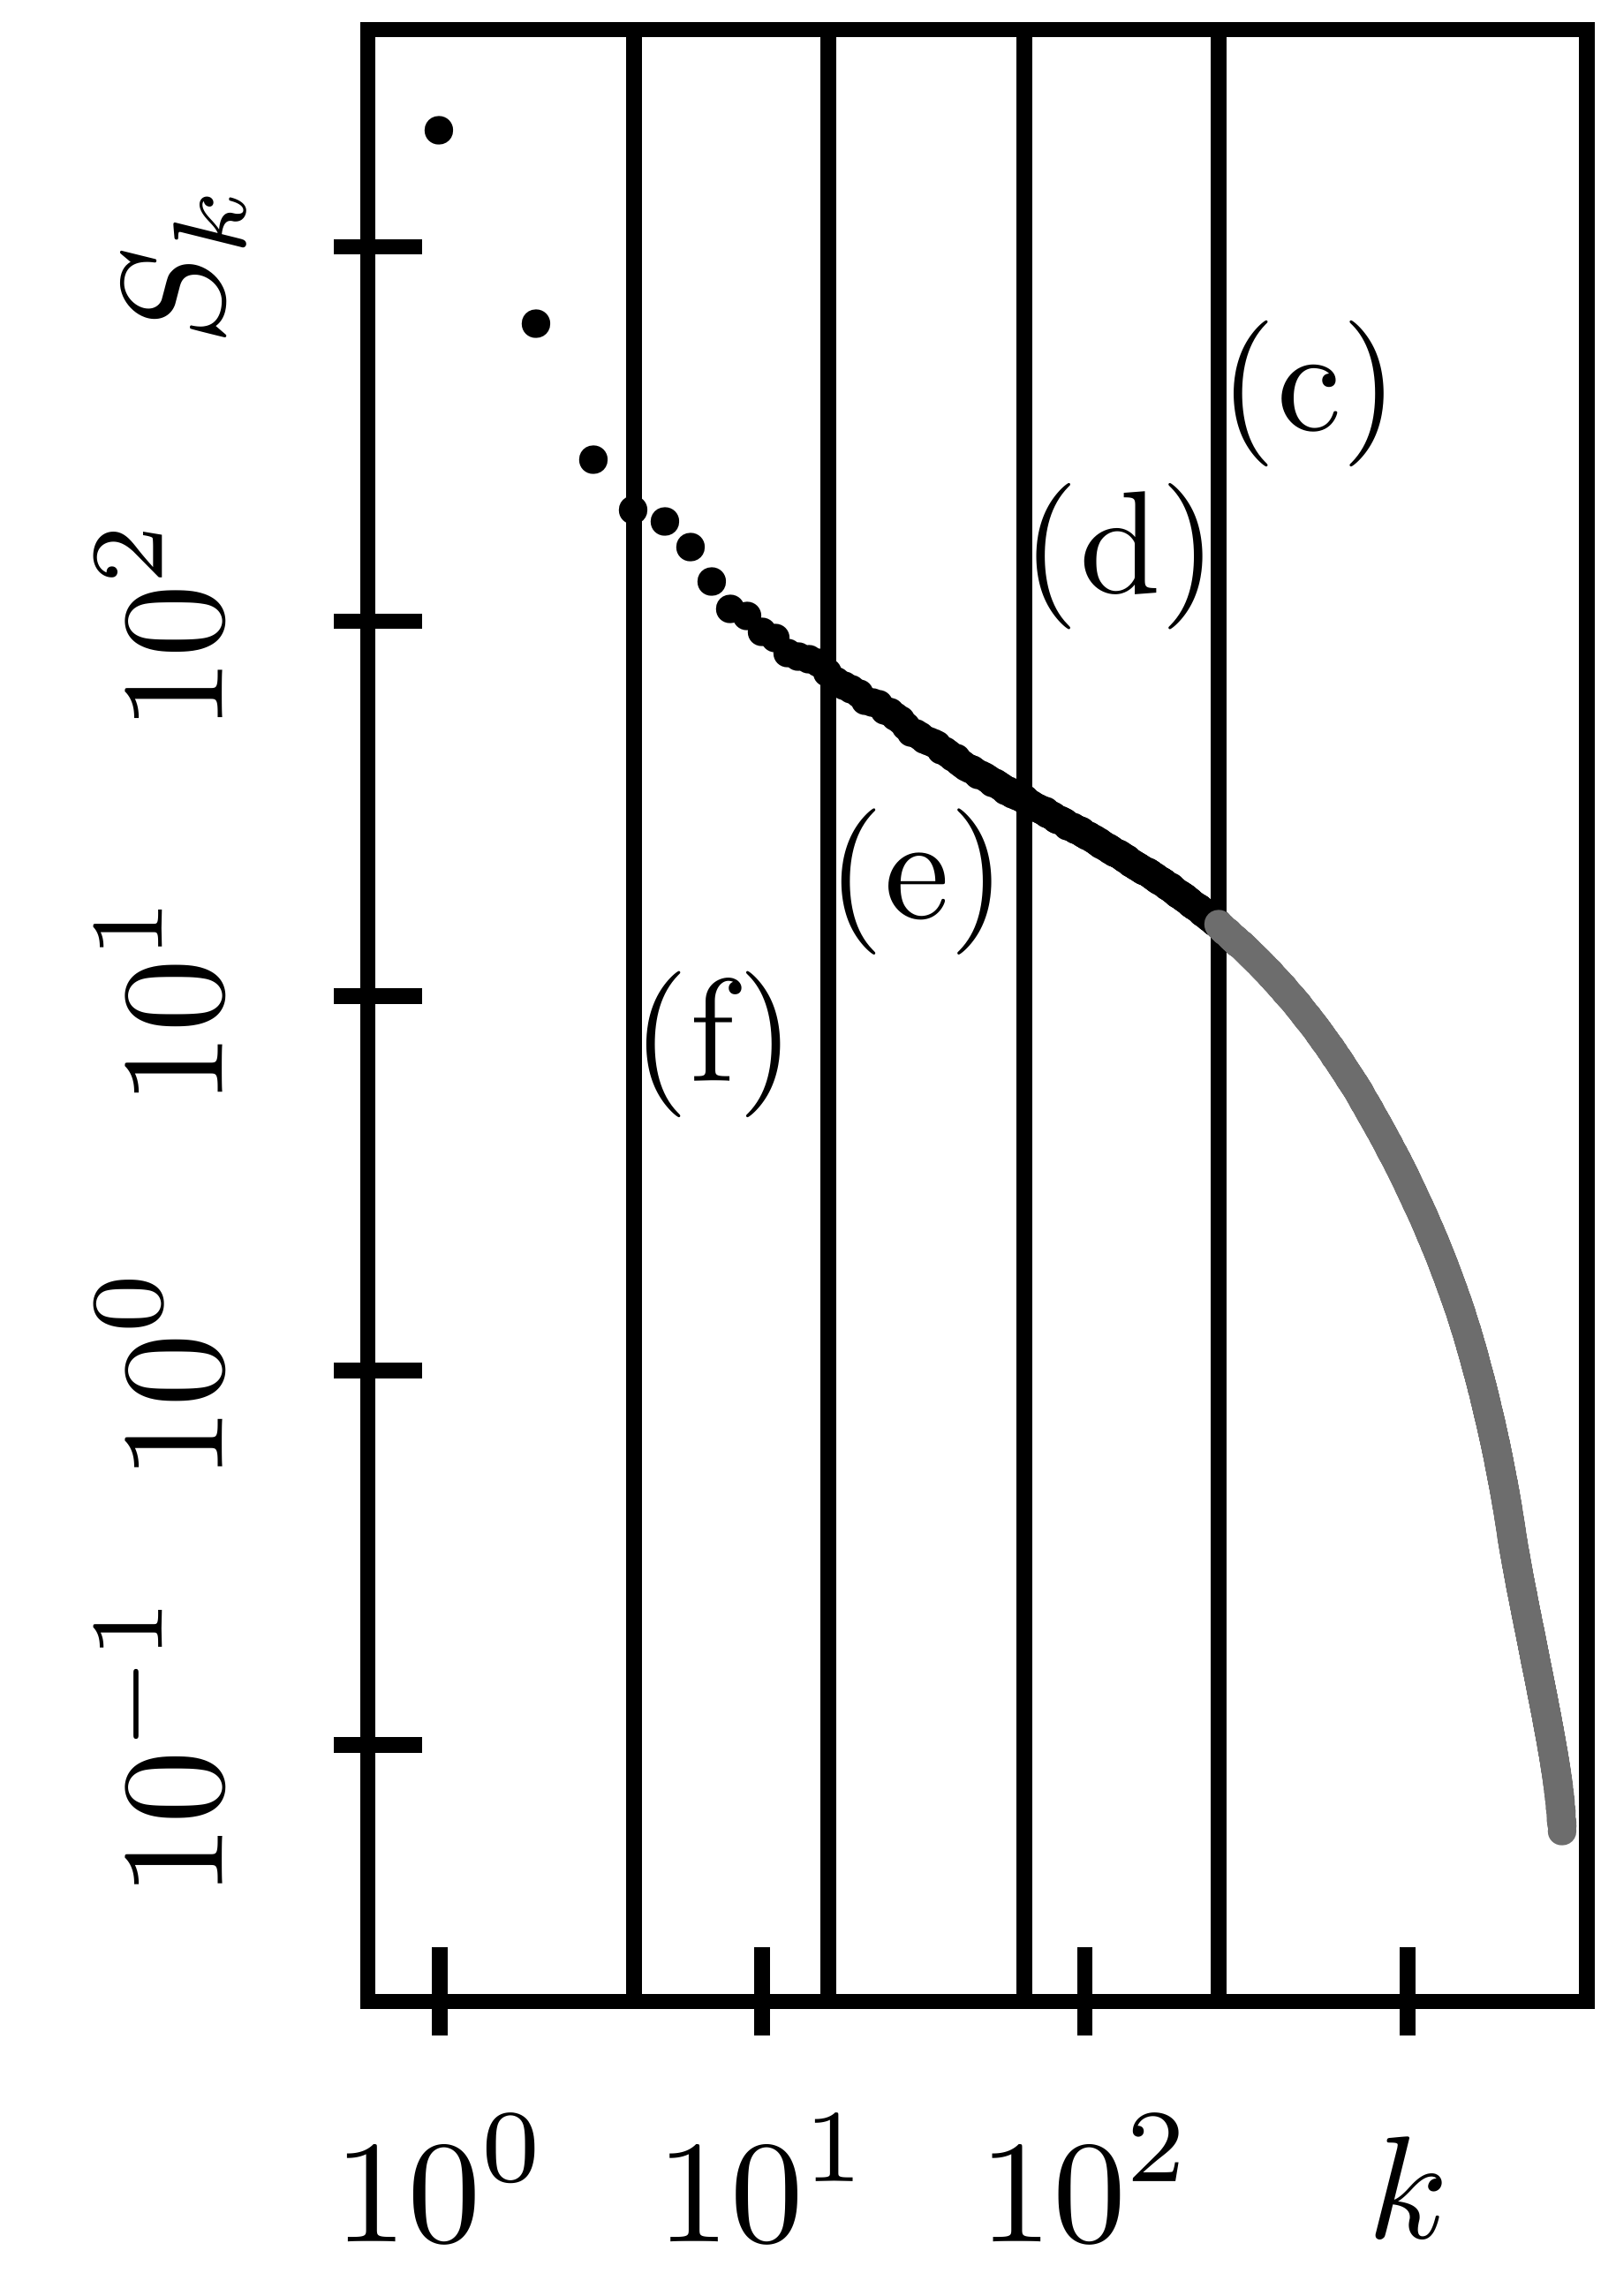
\includegraphics{figures/beach_singular_values.png}}
    \hfil
    \subfigure[]{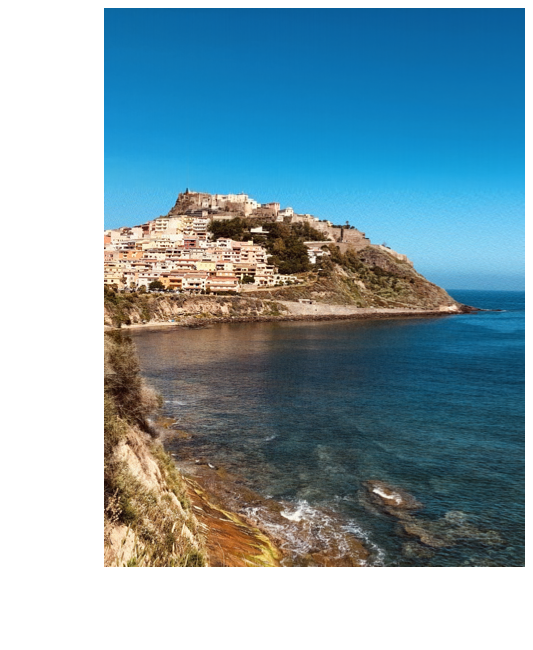
\includegraphics{figures/SVD_compressed.png}}
    \caption{(a) Uncompressed picture of Castelsardo (Sardinia, IT).
    The digital picture consists of $n_y\times n_x=3024\times2276$ pixels. (b) Singular values of the matrix $P_{i,(jc)}$ representing the picture. (c) Keeping the $250$ largest singular values still yields a good approximation of the uncompressed picture and requires only $19.3\%$ of the original storage space.}
    \label{fig:svd_image_compression}
\end{figure}
If the singular/spectral values are ordered, a truncation of the $\Lambda$ matrix neglects subdominant left and right eigenvectors of the original object and as such approximates the original matrix.
In case of a subsequent normalization to the original trace, the truncation process can be understood as a compression or tensor renormalization scheme.
The number of singular values kept in the approximation is thus naturally linked to the accuracy of the numerical renormalization.
Assume the picture to be of dimensions $\dim(P)=p_y\times p_x\times 3$, then keeping $m$ singular values implies that we need to store only a fraction of the matrices $U$ and $V^\dag$ to approximate the original picture $P$.
Assuming that the matrix $M\equiv \{P_{y,(x,c)}\}_{y,x,c}$ is of dimension $n_y=p_y$ times $n_x=3p_x$, the following visualization highlights the SVD
\begin{align}
    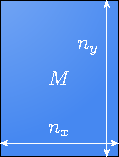
\includegraphics[valign=c]{figures/svd_mmat.pdf}
    =
    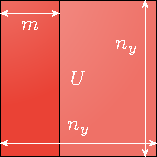
\includegraphics[valign=c]{figures/svd_umat.pdf}
    \
    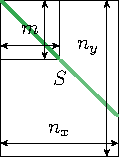
\includegraphics[valign=c]{figures/svd_smat.pdf}
    \
    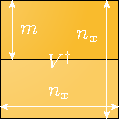
\includegraphics[valign=c]{figures/svd_vmat.pdf}.
    \label{eq:compression_scheme}
\end{align}
If we limit to $m$ spectral values, we only need to store $n_y\cdot m$ elements from $U$, $m$ singular values and $m\cdot n_x$ elements from $V^\dag$.
In total, we thus arrive at a compression rate
\begin{align}
    C_m = \frac{(n_x+n_y+1)m}{n_x n_y},
\end{align}
which allows for a high compression in case of a large and dense matrix $M$.
To give an example, I present the impact of compression in \cref{fig:svd_image_compression}.
Panel (a) denotes an uncompressed picture, the singular values of the digital picture presented in (b), and the result of keeping $250$ singular values as an approximation to the full picture, presented in (c).
The approximated picture yields a compression rate of roughly $19\%$, and visible differences to the original are negligible (if you look closely, the compressed figure appears to have some ``noise'' in the nice color gradient of the sky).
\\

The depicted compression scheme can actually be applied to quantum states.
Recall that any state can be expressed by a set of $L$ good quantum numbers, such that
\begin{align}
    \ket{\psi} = \sum_{i_1,i_2,\dots,i_L}C({i_1,i_2,\dots,i_L})\ket{i_1,i_2,\dots,i_L}
    \label{eq:generic_state}
\end{align}
and the collection of all $\ket{i_1,i_2,\dots,i_L}$ form a complete and orthonormal basis.
Note that the $L$-dimensional array $C$ depends on all internal quantum numbers and is thus exponentially large in the system size $L$ and the dimension of the quantum numbers $i_j$.
By the visual conventions, we may imagine the coefficients $C$ as a rank $L$ tensor, similar to the tensor $T$ discussed in \cref{eq:SVD_generalized}
\begin{align}
    C(i_1,i_2,\dots,i_L) \rightarrow C^{i_1,i_2,\dots,i_L} \equiv  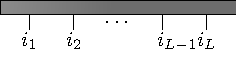
\includegraphics[valign=c]{figures/arbitrary_wavefunction.pdf}.
\end{align}
To account for the fact that the indices $\bm i$ are not fixed to specific values, I denote the dependence of the rank-$L$ tensor $C$ with square brackets.
To be more precise, if we fix the values for the quantum numbers $i_1,\dots,i_L$, the above equation is simply a scalar value.
This allows to apply the generalized SVD in a sequential manner:
Starting with the decomposition spanned by the bipartition of the first (last) leg, keeping the left (right) isometry and shifting the right (left) isometry to the adjacent leg position, is possible to decompose $C$ into a product of isometries with a single $\Lambda$ matrix in between two arbitrary leg positions $\ell,\ell+1$.
The necessary decomposition sequence is most easily reformulated in graphical notation
\begin{align}
    C^{i_1,i_2,\dots,i_L} \equiv 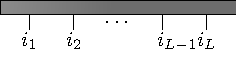
\includegraphics[valign=c]{figures/arbitrary_wavefunction.pdf}
    =
    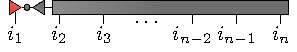
\includegraphics[valign=c]{figures/arbitrary_wavefunction_partially_decomposed_1.pdf}
    \\
    =
    \includegraphics[valign=c]{figures/arbitrary_wavefunction_partially_decomposed_2.pdf}
    \\
    =
    \includegraphics[valign=c]{figures/arbitrary_wavefunction_partially_decomposed_3.pdf}
    \\
    =\includegraphics[valign=c]{figures/arbitrary_wavefunction_decomposed.pdf}
    \label{eq:move_the_lambda_matrix}
\end{align}
in which at each step the three gray tensors are contracted before performing the next SVD.
This particular decomposition of a generic quantum state, i.e.
\begin{align}
    C^{i_1,i_2,\dots,i_L} \equiv \includegraphics[valign=c]{figures/arbitrary_wavefunction_decomposed.pdf}
    \label{eq:mixed_canonical_form}
\end{align}
is called the (mixed) canonical form of an MPS.
In other words, it represents the Schmidt decomposition of the state $\ket{\psi}$ in the subspaces $\HS_{A(\ell)}$ and $\HS_{B(\ell)}$ spanned by the first $\ell$ and last $L-\ell$ quantum numbers i.e.
\begin{align}
    \ket\psi = \sum_{\bm i} C^{\bm i}\ket{\bm i} = \sum_{k}s_{k}(\ell)\ket{\psi_{A(\ell),k}}
    \ket{\psi_{B(\ell),k}}
    \label{eq:schmidt_decomposition}
\end{align}
in which the transformed states $\ket{\psi_{A/B,k}}$ are given by the SVD-decomposed coefficient tensor
\begin{align}
    \ket{\psi_{A(\ell),k}}
    &=
    U^{i_1}_{k_1} U^{i_2}_{k_1,k_2}U^{i_3}_{k_2,k_3}\dots U^{i_\ell}_{k_{\ell-1},k}\ket{i_1,i_2,i_3,\dots,i_j}
    =\prod_{k=1}^\ell U^{[i_k]}\ket{i_1,\dots,i_\ell},\\
    %
    \ket{\psi_{B(\ell),k}}
    &=
    {V^\dag}^{i_{\ell+1}}_{k,k_{\ell+1}} {V^\dag}^{i_{\ell+2}}_{k_{\ell+1},k_{\ell+2}}\dots {V^\dag}^{i_L}_{k_{L-1}}\ket{i_{\ell+1},\dots,i_L}
    =
    \prod_{k=\ell+1}^L V^{\dag[i_k]}\ket{i_{\ell+1},\dots,i_L}.
    \label{eq:bipartition_orthonormal_basis}
\end{align}
In the two expressions above, I conveniently use the sum convention.
Additionally, from now on I use the convention that an object $T^{[i_1,\dots,i_n]}$ is a rank-$(n+2)$ tensor with two auxiliary (horizontal) links which depends on the collection of some physical quantum numbers $\bm i$.
Note that the position of the central matrix in \cref{eq:mixed_canonical_form} is not fixed to the center of the chain.
It can be moved arbitrarily to the right (left) by a sequence of singular value decompositions
\begin{align}
    \Lambda(\ell) V^{\dag[i_{\ell+1}]}V^{\dag[i_{\ell+2}]} &= U^{[i_{\ell+1}]}\Lambda(\ell+1) \tilde V^{\dag[i_{\ell+1}]}
    \equiv
    \includegraphics[valign=c]{figures/fMPS_3_1.pdf}
    =
    \includegraphics[valign=c]{figures/growing_5.pdf},
    \\
    U^{[i_{\ell-1}]}U^{[i_{\ell}]}\Lambda(\ell) &= \tilde U^{[i_{\ell-1}]}\Lambda(\ell-1) \tilde V^{\dag[i_{\ell}]}
    \equiv
    \includegraphics[valign=c]{figures/fMPS_4_1.pdf}
    =
    \includegraphics[valign=c]{figures/growing_5.pdf}.
\end{align}
Due to its fundamental importance for the remaining section, I will from now on use the notation
\begin{align}
    \ket\psi = \brlr{\prod_{k=1}^\ell U^{[i_k]}}\Lambda(\ell)\brlr{\prod_{k=\ell+1}^L V^{\dag[i_k]}}\ket{i_1,i_2,\dots,i_L}
\end{align}
to denote the mixed canonical decomposition of the coefficient tensor $C$ with rank-$3$ isometries ${U^{[i_k]}/V^{\dag[i_k]}}$ and a matrix $\Lambda(\ell)$ containing the Schmidt values of the bipartition after site $\ell$.
It is now obvious that (i) any quantum state can be decomposed into an MPS, (ii) that each MPS can be brought into the mixed canonical form and (iii) that MPS have a large gauge degree of freedom.
Point (iii) is clear from the fact that one may sandwich infinitely many identities in the MPS (each written as a product of two unitary matrices) which may in general rotate the colored isometry tensors, but leave the overall state invariant.
%
%
%%%%%%%%%%%%%%%%%%%%%%%%%%%%%%%%%%%%%%%%%%%%%%%%%%%%
\section{Reduced density matrix and Rényi entropy}
\label{sec:reduced_density_matrix_and_renyi_entropy}
%%%%%%%%%%%%%%%%%%%%%%%%%%%%%%%%%%%%%%%%%%%%%%%%%%%%
%
%
To understand the influence of the compression scheme, consider the way a generic density matrix is expressed in terms of a canonical MPS:
\begin{align}
    \hat\rho = \ket{\psi}\bra{\psi} = \sum_{k,k'}s_ks_{k'}\ket{\psi_{A,k},\psi_{B,k}}\bra{\psi_{A,k'},\psi_{B,k'}}.
\end{align}
Now imagine to compute the reduced density matrix of a bipartition formed by a block $A(\ell)$ of the first $\ell$ quantum numbers and a block $B(\ell)$ of the remaining ones.
A trace over the complement states of the partition $A/B$ gives the reduced density matrix in block $A/B$, i.e.
\begin{align}
    \hat\rho_A = \tr_B(\hat\rho)
    &=
    \sum_{k,k',k''}
    s_ks_{k'}
    \braket{\psi_{B,k''}|\psi_{A,k},\psi_{B,k}}\braket{\psi_{A,k'},\psi_{B,k'}|\psi_{B,k''}}
    =
    \sum_k s_k^2 \ket{\psi_{A,k}}\bra{\psi_{A,k}},\nonumber\\
    %
    \hat\rho_B = \tr_A(\hat\rho)
    &=
    \sum_k s_k^2 \ket{\psi_{B,k}}\bra{\psi_{B,k}}.
\end{align}
Note that normalization of the quantum state $\ket\psi$ implies $\tr\rho=\sum_k s_k^2=1$ and $s_k^2$ can be interpreted as the probability of state $\ket{\psi_{A/B,k}}$ contributing to the reduced density matrix $\hat\rho_{A/B}$.
The reduced density matrix is thus diagonal in the Schmidt decomposition, and solely determined by the spectral values $s_k$.
Imagine now to approximate the state $\ket\psi$ with a state $\ket{\psi'}$ by limiting the number of different $s_k$ in the bipartition $A,B$ such that the $m$ largest spectral values are kept in $\ket{\psi'}$ and the rest is set to zero.
Normalization of the state $\ket{\psi'}$ requires that $\sum_{k=1}^m {s'_k}^2$ must be renormalized to unity, which is satisfied if $s_k'=s_k/\sqrt{\sum_{l=1}^m s_l^2}$.
The threshold $m$ is thus directly related to approximating the reduced density matrix $\hat \rho_{A/B}$ with the $m$ most likely states in the Schmidt decomposition of a given bipartition $A/B$.
Please note that $s_k\equiv s_k(\ell)$ refers to the $k$'th singular value of a particular bipartition $A(\ell)/B(\ell)$, which considers the first/last $\ell/L-\ell$ quantum numbers.
% Therefore, it can be appropriate to denote this dependence also in the spectral values if needed, i.e. $s_k = s_k(\ell)$.
If we keep the $m$ largest singular values $s_k(\ell)$, $k\in\{1,2,\dots,m\}$ for any block size $\ell$, $m$ is a global property of MPS called the bond dimension.
\\

Density matrices are naturally related to the generalized Gibbs entropy for quantum states
\begin{align}
    S_1(\ell) = -\tr(\hat\rho_A\log\hat\rho_A) = -\tr(\hat\rho_B\log\hat\rho_B) = -\sum_k s^2_k\log(s^2_k)
\end{align}
which is a straightforward measure for the shared information between the bipartition, in information theory perspectives often called Shannon entropy of communication.
In this context, $-\log(s^2_k)$ is understood as the information content (or surprisal) of the Schmidt state, and $S_1$ is simply the expectation value of surprisal.
Such definition is readily understood from an experimentalist's point of view: measuring a state of very low spectral weight are surprizing, whereas likely quantum states bear a low surprise.
In a quantum physics audience, the entropy $S_1$ is commonly referred to as von Neumann entropy, and I denote it as $S_1$ because of its relation to the Rényi entropy -- a generalized version of the Shannon entropy
\begin{align}
    S_\alpha(\ell) = \frac{1}{1-\alpha}\tr\log\rho^\alpha_A
\end{align}
in the limit $\alpha\rightarrow1$.
The derivation of the limit is infrequently presented in the literature, but straightforward by using the Schmidt decomposition and L'Hôpital's rule
\begin{align}
    S_1(\ell)
    =
    \lim_{\alpha\rightarrow1}\frac1{1-\alpha}\tr\log\hat\rho_A^\alpha
    =
    -\lim_{\alpha\rightarrow1}\partial_\alpha\log\sum_k s_k^{2\alpha}
    =
    -\lim_{\alpha\rightarrow1}\frac{\sum_k\partial_\alpha s_k^{2\alpha}}{\sum_k s_k^{2\alpha}}
    =
    -\lim_{\alpha\rightarrow1}\sum_k \re^{\alpha\log s_k^2}
    \\
    =
    -\lim_{\alpha\rightarrow1}\sum_k \re^{\alpha\log s_k^2}\log s_k^2
    =
    -\sum_k s_k^2\log s_k^2
    =
    -\tr \hat\rho_A\log\hat\rho_A.
\end{align}
In conclusion, using MPS techniques in the canonical form provides immediate access to the information content of a given bipartition.
Note that the maximum entropy of an MPS is always restricted by the bond dimension $m$, i.e. $S_1(\ell)<\log(m)$.
%
%
%%%%%%%%%%%%%%%%%%%%%%%%%%%%%%%%%%%%%%%%%%%%%%%%%%%%%%%%%
\section{Scaling relations of the entanglement entropy}
\label{sec:scaling_relations_of_the_entanglement_entropy}
%%%%%%%%%%%%%%%%%%%%%%%%%%%%%%%%%%%%%%%%%%%%%%%%%%%%%%%%%
%
%
All of the discussion so far would not be very exciting for a wholehearted physicist, were it not for its close relation to quantum entanglement.
The phenomenon was firstly noted in $1935$ by Albert Einstein, Boris Podolsky, and Nathan Rosen~\cite{EPR1935}, also Erwin Schrödinger~\cite{Schrdinger1935,Schrdinger1936}, describing what is famously known as the EPR paradox~\cite{Reid2009}.
At its heart, it describes a group of particles interacting such that the quantum state of each individual particle cannot be described independently of the state of the others in the group.
The paradox part in the aforementioned works is described by quantum measurements performed on individual particles, which leads to irreversible collapses of the wave function and an alteration of the original quantum state of the other particles in the group.
Surprisingly, the phenomenon is independent of the distance between the particles and forms thus a unique form of correlations exclusively present in quantum systems.
\\

To make an example, consider the two-particle pure state $\ket{\psi}=\frac1{\sqrt2}\brlr{\ket{\uparrow\downarrow}+\ket{\downarrow\uparrow}}$ and the two particles being localized at two distant spacial positions.
In case we prepare a projective measurement of the first particle being in the $\uparrow$-state, the probability of the outcome is obviously $1/2$ and we end up with a collapsed post-measurement state of the form $\ket{\tilde\psi} = \ket{\uparrow\downarrow}$.
At the time of the measurement, the second particle collapses to the perfectly correlated alignment, and it does so immediately, independent on the spacial distance between the two parties.
A subsequent measurement of the second particle will thus yield $\downarrow$ with probability $1$.
Note that this instantaneous action does not violate causality since the outcome of the first measurement is random and as such cannot be used to transmit information.
With this example in mind, let us now encapsulate the definition of $N$-partite separable and entangled for states with $N$ individual particles.
\\

A state $\ket{\psi}$ is called $N$-partite separable iff. it can be written as a product of $N$ subsystems~\cite{Horodecki2009}
\begin{align}
    \ket{\psi} = \ket{\psi_1}\otimes\ket{\psi_2}\otimes\dots\otimes\ket{\psi_N}.
    \label{eq:separable_states}
\end{align}
Note that this expression is fundamentally different from the coherent superposition of exponentially many state vectors encountered in generic states (compare to ~\cref{eq:generic_state}).
As such, we call a state entangled, if it cannot be decomposed according to~\cref{eq:separable_states}.
The earlier example of a bipartite system is an element of the Bell basis, which are sometimes called ERP states
\begin{align}
    \ket{\psi^\pm}=\frac 1{\sqrt2}\brlr{\ket{\uparrow\downarrow}\pm\ket{\downarrow\uparrow}}
    \quad
    \ket{\phi^\pm}=\frac 1{\sqrt2}\brlr{\ket{\uparrow\uparrow}\pm\ket{\downarrow\downarrow}}
\end{align}
and they all have remarkable properties, first recognized by Schrödinger -- if one measures only one of the states, one finds it with equal probability in either $\ket{0}$ or $\ket{1}$.
As such, they give no information about the subsystems, whereas they are still pure and thus reveal full information about the global system.
The Bell states are special cases of bipartite maximally entangled states~\cite{Horodecki2009} and as such great examples to explore the entropic manifestation of entanglement.
In particular, it has been shown that the von Neumann entropy of a subsystem can be greater than the entropy of the global system iff. the state is entangled~\cite{Horodecki1994}.
The inequality for separable states can thus be expressed as $S(B|A)=S(\hat\rho)-S(\hat\rho_{A/B})\geq0$ with $\hat\rho$ the density matrix and $\hat\rho_{A/B}$ the reduced density matrix of bipartition $A/B$.
As such, the von Neumann entropy serves as a scalar separability criteria, in analogy to the Bell inequalities.
The discussions of entangled states breaking the positivity of $S(A|B)$ reach far beyond the present aim of this introduction \cite{Horodecki2006}, and I simply conclude here that the von Neumann entropy is a useful scalar measure of bipartite entanglement.
\\

Coming back to the connection to MPS with finite bond dimension, we now know that the upper bound restriction of the entropy limits the available entanglement of the approximation.
This, in turn, does not provide an explanation why such an approximation should not ``go wrong quickly'' in a sense that the important properties of the approximated state are lost, even if the bond dimension is large.
Incidentally, at the time DMRG was introduced by Steven White~\cite{White1992}, the success of the renormalization scheme remained a mystery.
Some insights were concluded by the derivation of universal scaling laws of the entropy provided e.g. by Calabrese and Cardy in 2004~\cite{Calabrese2004} in proximity of a quantum critical point.
In 2007, Hastings published his famous proof of the area law for one-dimensional quantum systems~\cite{Hastings2007}.
In its essence, it provides an upper bound to the von Neumann entropy for gapped and local (i.e. no long-ranged interactions) Hamiltonians scaling as the area ($\equiv$ a constant) of one-dimensional systems.
Essentially, the works can be summarized by the following two statements~\cite{Eisert2010}:
Consider a block of $1,2,\dots,\ell$ particles with internal dimension $D$, the entanglement entropy of the physically relevant part (i.e. the low-energy subspace of $\HS$) scales as
\begin{align}
    S_1(\ell) &= \frac c{3b}\log[d(\ell)],\text{ if the system is critical}\\
    S_1(\ell) &= c_0\xi\log\brlr{6\xi}\log D2^{6\xi\log D},\text{ if the system is local and gapped with $\Delta E>0$}
\end{align}
in which $c_0$ is a constant of order one, $\xi=\max(2v/\Delta E,\xi_C)$ is the correlation length, $v$ the velocity of sound, $\xi_C$ of order one and $d(\ell)$ encodes the size of the block.
For periodic ($b=1$) and open ($b=2$) boundary conditions, $d(\ell)$ is the chord distance encoding the length of a semi-circle
\begin{align}
    d(\ell) = \left|\frac L\pi\sin(\pi/L\ell)\right|.
\end{align}
The main messages is that, for gapped systems, physically relevant states live in the low-entangled subspace of the full Hilbert space.
This implies that the MPS Ansatz is an optimal choice to target the low-lying excitations of the full many body Hilbert space, which, in turn, follow an area law of entanglement.
%
%
%%%%%%%%%%%%%%%%%%%%%%%%%%%%%%%%%%%%%%%%%%%%%%%%%%%%%%%%%%%
\section{Matrix product operators and expectation values}
\label{sec:matrix_product_operators_and_expectation_values}
%%%%%%%%%%%%%%%%%%%%%%%%%%%%%%%%%%%%%%%%%%%%%%%%%%%%%%%%%%%
%
%
Let us now understand the action of operators in the basis of MPS.
Consider a local operator acting on site $q$, which can be written in general as $\hat o_q = \sum_{i_q',i_q''}o_{i_q',i_q''}\ket{i_q'}\bra{i_q''}$.
Its action on the canonical form of an MPS can be expressed as
\begin{align}
    \hat o_q\ket\psi &= \sum_{i_1,i_2,\dots,i_q,\dots,i_L}\sum_{i_q'}o_{i_q',i_q} C^{i_1,i_2,\dots,i_q,\dots,i_L}\ket{i_1,i_2,\dots,i_{q-1},i_q',i_{q+1},\dots,i_L}
    \\
    &= \sum_{i_1,i_2,\dots,i_L}\tilde C^{i_1,i_2,\dots,i_L}\ket{i_1,i_2,\dots,i_L}
\end{align}
and we note that it leaves the overall form of the MPS invariant.
In particular, it acts as a contraction between the $o$-matrix and the $q$'th vertical leg of the $C$-tensor, according to
\begin{align}
    \tilde C^{i_1,i_2,\dots,i_L} = \sum_{i_q'}o_{i_q,i_q'}C^{i_1,i_2,\dots,i_q',\dots,i_L}.
\end{align}
Therefore, we can represent any local operator as a rank-$2$ tensor composed by the matrix elements of $\hat o$.
The same reasoning applies for operators acting on $p$ sites -- they are represented by rank-$2p$ tensors containing the entries of the matrix elements, contracted with the $p$ corresponding vertical links of the $C$-tensor.
Such an object is then called matrix product operator (MPO) which allow the efficient representation of generic Hamiltonians.
\\

The derivation of the MPO representation of a given Hamiltonian is actually straightforward, since it is the typically a sum of products of local operators, which, as we now know, each have a MPO representation.
Consider for example the Ising model
\begin{align}
    \hat H = \hat H_{h} + \hat H_{J},
    \quad
    \hat H_{J} = J\sum_{i=\ell}^{L-1}\hat X_\ell \hat X_{\ell+1},
    \quad
    \hat H_{h} = h\sum_{\ell=1}^{L}\hat Z_\ell,
\end{align}
in which $\hat X/\hat Y/\hat Z$ denote the spin-1/2 operators.
They have the following representations
\begin{align}
    \hat X_\ell/\hat Y_\ell/\hat Z_\ell = \sum_{i_\ell,i'_\ell\in\{\uparrow,\downarrow\}}X_{i_\ell,i_\ell'}/Y_{i_\ell,i_\ell'}/Z_{i_\ell,i_\ell'}\ket{i_\ell}\bra{i'_\ell},
\end{align}
in which $X/Y/Z$ are the spin-1/2 Pauli matrices
\begin{align}
    X =
    \begin{pmatrix}
        0 & 1 \\
        1 & 0
    \end{pmatrix}
    ,
    \quad
    Y =
    \begin{pmatrix}
        0 & -\ri \\
        \ri & 0
    \end{pmatrix}
    ,
    \quad
    Z =
    \begin{pmatrix}
        1 & 0 \\
        0 & -1
    \end{pmatrix}.
\end{align}
The additional subscript $\ell$ denotes an isolated action of $\hat X_\ell/\hat Y_\ell/\hat Z_\ell$ on the $\ell$'th spin of the system.
Note that the Hamiltonian can be recast into a product of bulk $\ell\neq1,L$ operators of the form
\begin{align}
    \hat W_\ell =
    \begin{pmatrix}
        \hat{\mathbb 1}_\ell & \hat X_\ell & \hat Z_\ell\\
         0 & 0 & \hat X_\ell\\
        0 & 0 & \hat{\mathbb 1}_\ell\\
    \end{pmatrix}
\end{align}
representing a set of local operators acting locally on a single site.
The multiplication of the $\hat W_\ell$ matrix operators does not yield the desired result immediately, which is readily solved by a slight modification of the boundary operators
\begin{align}
    \hat W_1 =
    \begin{pmatrix}
        1 & 0 & 0
    \end{pmatrix}
    \begin{pmatrix}
        \hat{\mathbb 1}_1 & \hat X_1 & \hat Z_1\\
        0 & 0 & \hat X_1\\
        0 & 0 & \hat{\mathbb 1}_1\\
    \end{pmatrix}
    =
    \begin{pmatrix}
        \hat{\mathbb 1}_1 & \hat X_1 & \hat Z_1
    \end{pmatrix}
    ,
    \quad
    \hat W_L =
    \begin{pmatrix}
        \hat{\mathbb 1}_L & \hat X_L & \hat Z_L\\
        0 & 0 & \hat X_L\\
        0 & 0 & \hat{\mathbb 1}_L\\
    \end{pmatrix}
    \begin{pmatrix}
        0 \\ 0 \\ 1
    \end{pmatrix}
    \begin{pmatrix}
        \hat Z_L\\
        \hat X_L\\
        \hat{\mathbb 1}_L\\
    \end{pmatrix}
    \label{eq:boundary_W}
\end{align}
such that the global Hamiltonian is given by the product
% \begin{align}
%     \hat X_i\hat X_{i+1} + \hat Z_i + \hat Z_{i+1} = \hat W_l \hat W_i \hat W_{i+1} \hat W_r
% \end{align}
% and as such
\begin{align}
    \hat H = \prod_{\ell=1}^{L}\hat W_{\ell}.
\end{align}
Since $\hat W_\ell$ contains a set of local operators which each have an MPO representation, the action of the Hamiltonian on a state $\ket\psi$ can be understood as a product of rank-$4$ tensors $W^{[i_\ell',i_\ell]}$ containing the matrix elements of $\hat W_{\ell}$.
In particular, one obtains the following tensorial representation, acting on a single site $\ell\neq1,L$ of the bulk
\begin{align}
    W^{[i_\ell',i_\ell]} =
    \begin{pmatrix}
        \delta_{i_\ell',i_\ell} & X_{i_\ell',i_\ell} & Z_{i_\ell',i_\ell} \\
        0 & 0 & X_{i_\ell',i_\ell} \\
        0 & 0 & \delta_{i_\ell',i_\ell}
    \end{pmatrix}
    .
\end{align}
It is straightforward to introduce two additional rank-$3$ boundary tensors, in equivalence to \cref{eq:boundary_W}.
The MPO representation $W$ of the Hamiltonian $\hat H$ is very versatile -- any Hamiltonian can be recast into a set of matrix product operators that are upper triangular, even if the interactions are long-ranged or spacially dependent, e.g. in the case of disorder.
Note that the MPO form is not limited to spin systems due to the famous Jordan-Wigner transformation.
It is defined in terms of the ladder operators with matrix representations $\hat\sigma^\pm = \frac12(\hat X\pm\ri \hat Y)$, i.e.
\begin{align}
    \hat a_i^\pdag = \brlr{\prod_{j<i}-\hat Z}\hat\sigma^-_i,
    \qquad
    \hat a_i^\dag = \brlr{\prod_{j<i}-\hat Z}\hat\sigma^+_i.
\end{align}
This way, the fermionic creation and annihilation operators are represented by spin ladder operators.
To restore the anticommutation relations of fermions, the additional phase string is required.
Note that the presence of the string of $\hat Z$'s in general imposes long-ranged interactions in two-dimensional systems, such that a direct application of the Jordan-Wigner transformation is primarily used in (quasi) one-dimensional systems~\cite{Franchini2017}.
%
%
%%%%%%%%%%%%%%%%%%%%%%%%%%%%%%%%%%%%%%%%%%%
\section{Variational ground state search}
\label{sec:variational_ground_state_search}
%%%%%%%%%%%%%%%%%%%%%%%%%%%%%%%%%%%%%%%%%%%
%
%
The original variational ground state search is formalized in the density matrix renormalization group (DMRG), introduced by Steven White in 1992~\cite{White1992}.
In it's essence, it is a numerical optimization scheme targetting the low energy sector of a given system.
Nowadays, it is understood as an MPS Ansatz of the trial wavefunction in which at each iteration a few local tensors (in most cases one or two) are variationally optimized.
For the numerical simulations employed in all of our articles, I implemented two optimization schemes, which are then combined to find an optimal MPS approximation for finite systems.
The first one is the growing algorithm (sometimes dubbed iDMRG), which is most useful to construct the trial wavefunction of the second scheme, namely traditional DMRG reformulated in the language of MPS~\cite{Schollwoeck2011,Silvi2019}.
\\

Consider the way the energy expectation value is written in the MPS language: it is a sandwich of the product of $W$ tensors (the local MPO representing the Hamiltonian) with the trial wavefunction.
To find the groundstate, we extremize the energy
\begin{align}
    E = \min_{\ket{\psi}}\braket{\psi |\hat H | \psi}
\end{align}
under the constraint that $\braket{\psi|\psi}=1$.
Using a Lagrange multiplier, the equation becomes
\begin{align}
    \braket{\psi|\hat H|\psi} - \lambda_\psi\brlr{\braket{\psi|\psi}-1} = 0.
    \label{eq:lagrangian_multiplier}
\end{align}
Now the MPS structure of $\ket\psi$ is exploited, and I decompose the state into the canonical form
\begin{align}
    \ket\psi
    =
    \brlr{\prod_{k=1}^{\ell}U^{[i_k]}}\Lambda(\ell)\brlr{\prod_{k=\ell+1}^{L}V^{\dag[i_k]}}\ket{\bm i}
    \equiv
    \includegraphics[valign=c]{figures/arbitrary_wavefunction_decomposed_decolorized.pdf}\ket{i_1,i_2,\dots,i_L}.
\end{align}
Please note that I use the sum convention in the above, and the tensors $U^{[i_k]}$ and $V^{\dag[i_k]}$ satisfy the isometry conditions
\begin{align}
    \sum_{i_k}U^{\dag[i_k]}U^{[i_k]} = \mathbb 1,
    \quad
    \sum_{i_k}V^{\dag[i_k]}V^{[i_k]} = \mathbb 1.
    \label{eq:isometry_tensors}
\end{align}
Diagrammatically, the two conditions exactly correspond to the two graphical contractions
\begin{align}
    \includegraphics[valign=c]{figures/left_isometry_tensor.pdf}
    =
    \includegraphics[valign=c]{figures/identity_tensor_left.pdf},
    \quad
    \includegraphics[valign=c]{figures/right_isometry_tensor.pdf}
    =
    \includegraphics[valign=c]{figures/identity_tensor_right.pdf}.
    \label{eq:isometry_tensors_diagram}
\end{align}
To cast \cref{eq:lagrangian_multiplier} into a variational problem for the tensors at position $\ell$ and $\ell+1$, it is convenient to use the graphical notation
\begin{align}
    \includegraphics[valign=c]{figures/lagrangian_multiplier_equation_1.pdf}
    -
    \lambda_\psi
    \brlr{\includegraphics[valign=c]{figures/lagrangian_multiplier_equation_2.pdf}-1}
    =
    0.
    \label{eq:lagrangian_multiplier_graphical}
\end{align}
In the above, I use square tensors to denote the local MPOs of the Hamiltonian.
I now proceed by the application of a gradient on both sides of \cref{eq:lagrangian_multiplier}, in which I derive with respect to the entries of the contraction of the red, black and blue tensor, i.e.
\begin{align}
    \nabla(\ell,\ell+1)_{kn}\equiv\frac\partial{\partial\brlr{U^{i_\ell}_{k,l}S_l V^{\dag i_{\ell+1}}_{l,n}}^*}.
\end{align}
Since the tensors enter in the equation in a linear fashion, the application of the gradient simply corresponds to removing the three tensors from the conjugate contraction (and of course the scalar $1$) in \cref{eq:lagrangian_multiplier_graphical}.
One arrives at the tensorial expression
\begin{align}
    \includegraphics[valign=c]{figures/lagrangian_multiplier_equation_3.pdf}
    =
    \lambda_\psi
    \includegraphics[valign=c]{figures/lagrangian_multiplier_equation_4.pdf}
    .
    \label{eq:lagrangian_multiplier_graphical_2}
\end{align}
This can be better understood after reshaping $U^{[i_\ell]}\Lambda(\ell) V^{\dag[i_{\ell+1}]}$ (the red, black and blue tensors in \cref{eq:lagrangian_multiplier_graphical_2}) to a vector ${\bm A}_C^{[i_\ell,i_{\ell+1}]}=f\circ U^{[i_\ell]}\Lambda V^{\dag[i_{\ell+1}]}$ of dimension $m^2D^2$, in which $f$ denotes the reshaping.
The contracted network of grey tensors should then be reshaped to a matrix $\bm H_{\rm eff.}^{[i_\ell',i_{\ell+1}',i_\ell,i_{\ell+1}]}$ of dimension $m^2D^2\times m^2D^2$.
The applied gradient then simply corresponds to $\nabla_{\bm A_C}$ and the tensorial expression in \cref{eq:lagrangian_multiplier_graphical_2} reduces to
\begin{align}
    \bm H_{\rm eff.}^{[i_\ell',i_{\ell+1}',i_\ell,i_{\ell+1}]}{\bm A}_C^{[i_\ell,i_{\ell+1}]} = \lambda_\psi {\bm A}_C^{[i_\ell',i_{\ell+1}']}.
    \label{eq:MPS_optimization}
\end{align}
It is now obvious that (i) the Lagrange multiplier $\lambda_\psi$ corresponds to the energy of the MPS and (ii) the equations span a standard eigenvalue problem for the vector $\bm A_C$ which can be solved efficiently for the end of the spectrum with libraries like ARPACK~\cite{Lehoucq1998}.
After the optimal low-energy vector is computed, it must be reshaped back to a tensor, and then decomposed through the generalized SVD to obtain the original canonical form of the MPS.
In particular, one performs the sequence
\begin{align}
    f^{-1}\circ {\bm A}_C^{[i_\ell,i_{\ell+1}]}
    \equiv
    \includegraphics[valign=c]{figures/growing_4_4.pdf}
    =
    \includegraphics[valign=c]{figures/growing_5.pdf}
    \equiv
    U^{[i_\ell]} \Lambda V^{\dag[i_{\ell+1}]}.
\end{align}
Note that the standard eigenvalue problem in \cref{eq:MPS_optimization} is promoted to a generalized eigenvalue problem if we would not rely on the normalized and canonical form of the MPS~\cite{Silvi2019}.
The aim now is to find the globally optimal vectors ${\bm A}_C$ for each site, which can be achieved in an iterative manner by the growing and finite MPS algorithm.
\\

A minimal example of the growing MPS algorithm is formalized as follows:
\begin{enumerate}
    \item Choose an even number $L$ corresponding to the final number of quantum numbers in the resulting quantum state.
    It is equal to twice the number of iterations.
    \item Set $n=1$. Compute the lowest energy vector ${\bm A}_C^{[i_1,i_2]}$ for a system of two sites only.
    The eigenvalue equation and graphical representation reads
    \begin{align}
        \bm H_{\rm eff.}^{[i_1',i_{2}',i_1,i_2]} {\bm A}_C^{[i_1,i_2]} &= \lambda_\psi {\bm A}_C^{[i_1',i_2']}\\
        \includegraphics[valign=c]{figures/two_site_problem_1.pdf}
        &=
        \lambda_\psi
        \includegraphics[valign=c]{figures/two_site_problem_2.pdf}\ ,
        \label{eq:two_site_problem}
    \end{align}
    in which the green tensor represents ${\bm A}_C$ and the two grey rank-$3$ tensors correspond to the boundary MPOs of the Hamiltonian.
    % Note that the two green tensors can also be understood as rank-$3$ tensors in which the additional horizontal link has dimension $1$.
    \item Use the generalized singular value decomposition depicted in \cref{eq:SVD_generalized} to decouple the two quantum numbers into a product of two isometries and a matrix $\Lambda$ containing the spectral values
    \begin{align}
        f^{-1}\circ {\bm A}_C^{[i_1',i_2']} &= U^{[i_1']}\Lambda V^{\dag[i_{L}']},
        \\
        \includegraphics[valign=c]{figures/two_site_problem_2.pdf}
        &=
        \includegraphics[valign=c]{figures/two_site_problem_2_decomp.pdf}\ .
    \end{align}
    Renormalize the truncated matrix $\Lambda$ such that $\tr(\Lambda^2)=1$.
    \item Grow the size of the MPS from $2n$ to $2n+2$ sites by replacing the central matrix $\Lambda$ with a rank-$4$ tensor of fitting dimensions
    \begin{align}
        \brlr{\prod_{k=1}^nU^{[i_k']}}\Lambda \brlr{\prod_{k=1}^{n}V^{\dag[i_{L+1-n}']}}
        &\longrightarrow
        \brlr{\prod_{k=1}^nU^{[i_k']}} T^{[i_{n+1},i_{L-n}]}\brlr{\prod_{k=1}^{n}V^{\dag[i_{L+1-n}']}},
        \\
        \includegraphics[valign=c]{figures/growing_4_1.pdf}
        &\longrightarrow
        \includegraphics[valign=c]{figures/growing_4_2.pdf}\ .
    \end{align}
    Then use \cref{eq:MPS_optimization} to variationally solve for the lowest energy vector ${\bm A}_C$ corresponding to the inserted (green) tensor
    \begin{align}
        {\bm H}_{\rm eff.}^{[i_{n+1}',i_{n+2}',i_{n+1},i_{n+2}]} {\bm A}_C^{[i_{n+1},i_{n+2}]} &= \lambda_\psi {\bm A}_C^{[i_{n+1}',i_{n+2}']}
        ,\\
        \includegraphics[valign=c]{figures/growing_4_3.pdf}
        &=
        \lambda_\psi
        \includegraphics[valign=c]{figures/growing_4_4.pdf}.
        \label{eq:two_site_problem}
    \end{align}
    \item Use the generalized singular value decomposition to decouple the two quantum numbers into a product of two isometries and a matrix $\Lambda$ containing the spectral values
    \begin{align}
        f^{-1}\circ \bm A_C^{[i_{n+1}',i_{n+2}']} &= U^{[i_{n+1}']}\Lambda V^{\dag[i_{L-n}']},
        \\
        \includegraphics[valign=c]{figures/growing_4_4.pdf}
        &=
        \includegraphics[valign=c]{figures/growing_5.pdf}.
    \end{align}
    Apply the compression scheme by keeping at most the $m$ largest singular values and renormalize the truncated matrix $\Lambda$.
    Increase $n\rightarrow n+1$. Go to step 4 or stop if $n=L/2$.
\end{enumerate}
The common application of the growing algorithm is two-fold.
It can be used naively to approximate the central tensors of a fully translationally invariant chain by sending $L\gg2$ to very large values.
The convergence is reached when the overlap between the optimal vectors $v(n,n+1)$ and $v(n-1,n)$ of the previous iteration step approaches a user-specified threshold.
This approach however requires the state to be fully translationally invariant over a single site.
A workaround of this issue is to relax the insertion of two sites in the center of the MPS to arbitrary many.
However, the convergence to the best thermodynamic MPS state is never achieved.
This is due to the intrinsically finite structure of the MPS in the growing algorithm which breaks translational symmetry at every step, and another Ansatz is required.
\\

One viable option is to approximate the (infinite) environments to the left and right of the central tensors with the dominant eigenstates of the transfer matrices.
The corresponding algorithm is then called infinite boundary conditioned MPS~\cite{Phien2012} or variational uniform MPS (VUMPS)~\cite{ZaunerStauber2018}.
In our works, we were mostly interested in the simulation of finite systems and I omit the description of such an implementation.
\\

The second application concerns the MPS obtained after $L/2$ steps -- it can serve as a trial state for a finite system of length $L$, which is refined by the finite MPS algorithm:
\begin{enumerate}
    \item Set $n=1$. Start with a trial MPS in the canonical form (e.g. acquired by the growing algorithm) and transform the MPS such that the $\Lambda$ matrix is between sites $1$ and $2$, i.e.
    \begin{align}
        C^{i_1,i_2,i_3,\dots,i_{L-1},i_L} \equiv \includegraphics[valign=c]{figures/fMPS_1.pdf}.
    \end{align}
    \item Compute the new lowest energy vector $\bm A_C$ according to \cref{eq:MPS_optimization}\footnote{Note that at the system's boundaries, ${\bm A}_C$ is effectively a rank-$3$ tensors and one of the isometries will be of rank-$2$.} and decompose it to two isometries and a matrix $\Lambda$ containing the singular values
    \begin{align}
        f^{-1}\circ \bm A_C^{[i_{n},i_{n+1}]} &= U^{[i_n]}\Lambda(n) V^{\dag[i_{n+1}]}\\
        \includegraphics[valign=c]{figures/growing_4_4.pdf}
        &=
        \includegraphics[valign=c]{figures/growing_5.pdf}
        .
    \end{align}
    Apply the compression scheme by keeping at most the $m$ largest singular values and renormalize the truncated matrix $\Lambda$.
    Proceed then with step $3$ (sweeping from left to the right) or step $4$ (sweeping from right to the left).
    \item If $n=L-1$ continue with step 4. Shift the matrix $\Lambda(n)$ to the next site by the decomposition
    \begin{align}
        \Lambda(n) V^{\dag[i_{n+1}]} V^{\dag[i_{n+2}]} &= U^{[i_{n+1}]}\Lambda(n+1)\tilde V^{\dag[i_{n+2}]}
        \\
        \includegraphics[valign=c]{figures/fMPS_3_1.pdf}
        &=
        \includegraphics[valign=c]{figures/growing_5.pdf}
        .
    \end{align}
    Increase $n\rightarrow n+1$ and go back to step 2.
    This is called sweeping from left to right.
    \item If $n=1$ continue with step 3. Shift the matrix $\Lambda(n)$ to the previous site by the decomposition
    \begin{align}
        U^{[i_{n-1}]}U^{[i_n]}\Lambda(n) &= \tilde U^{[i_{n-1}]}\Lambda(n-1) V^{\dag[i_n]}
        \\
        \includegraphics[valign=c]{figures/fMPS_4_1.pdf}
        &=
        \includegraphics[valign=c]{figures/growing_5.pdf}
        .
    \end{align}
    Decrease $n\rightarrow n-1$ and go back to step 2.
    This is called sweeping from right to the left.
\end{enumerate}
The finite MPS optimization is usually performed in so-called ``sweeps'', i.e. a full sweeping cycle from left to right is done for each site $n=1,2,\dots,L-1$, after which a full sweeping cycle from right to left $n=L-1,L-2,\dots,1$ is applied.
Iteratively optimizing the local tensors leads to a variational trajectory in the family of MPS with bond dimension $m$.
\\

As usual, the precise representatives of global extrema in optimization schemes remain unknown and its always possible to be trapped inside of local minima.
In such cases, viable estimates of the error are needed.
The error to an exact eigenstate of the Hamiltonian can be estimated in a straightforward manner by computing the variance of the approximation.
For cases in which the MPS is equivalent to an eigenstate of the full Hamiltonian, the variance will reduce to $0$. In general, however, the approximation is not a true eigenstate of the Hamiltonian and as such we arrive at
\begin{align}
    \varepsilon_H(m) = \sqrt{\braket{\psi(m)|\hat H^2|\psi(m)} - \braket{\psi(m)|\hat H|\psi(m)}^2}\geq 0.
\end{align}
The indication of the dependence on $m$ is reminiscent of the fact that $\varepsilon_H(m)$ typically depends on the bond dimension of the MPS.
It can then be checked if the variance converges to machine precision by performing a so-called bond dimension scaling analysis~\cite{Hubig2018}.
In case of a finite bond dimension analysis, $\varepsilon_H(m)$ serves as a measure of the approximation error.
Alternatively, the discarded weight of the singular values can serve as a measure of the error.
It is defined as
\begin{align}
    \varepsilon_\rho(m) = \sup_{\ell}\sum_{k=m}^\infty s_k(\ell)
\end{align}
in which $s_k(\ell)$ denotes the $k$'th singular value of the mixed-canonical representation of the MPS.
%
%
%%%%%%%%%%%%%%%%%%%%%%%%%%
\section{Time evolution}
\label{sec:time_evolution}
%%%%%%%%%%%%%%%%%%%%%%%%%%
%
%
There are several well-established methods used to simulate the time evolution of an initial MPS~\cite{Paeckel2019} and here I will focus on the time-dependent variational principle (TDVP).
The crucial difference to other algorithms is that it utilizes a backward evolution of the singular values in order to project the tensor onto its tangent space.
This way it aligns the variational trajectory to the tangent space of the MPS, leading to a particularly robust and efficient implementation compared to other algorithms~\cite{Haegeman2011}.
In addition, TDVP of a trial MPS in imaginary time is known to be identical to traditional DMRG/finite MPS, which leads to a unified framework for the time evolution and optimization of matrix product states~\cite{Haegeman2016}.
\\

Before I introduce the algorithm, we need a couple of prerequisites.
First, the MPS will be written in the mixed canonical gauge with a tensor $A_C$ (matrix $C$) which is not an isometry, i.e.
\begin{align}
    C^{i_1,i_2,\dots,i_\ell,\dots,i_L} &= \brlr{\prod_{k=1}^{\ell-1} U^{[i_k]}} A_C^{[i_\ell]} \brlr{\prod_{k=\ell+1}^{L} V^{\dag[i_k]}}
    \equiv
    &\includegraphics[valign=c]{figures/center_site_gauge.pdf},
    \\
    &=\brlr{\prod_{k=1}^{\ell} U^{[i_k]}} C(\ell) \brlr{\prod_{k=\ell+1}^{L} V^{\dag[i_k]}}
    \equiv
    &\includegraphics[valign=c]{figures/center_site_gauge_2.pdf}
    .
\end{align}
As usual, the tensors $U$ and $V^\dag$ are isometries which satisfy \cref{eq:isometry_tensors,eq:isometry_tensors_diagram}.
% Note that the center tensor can always be decomposed into a rank-$3$ isometry and a product of matrices
% \begin{align}
%     A_C^{[i_\ell]} = U^{[i_\ell]}C_R = C_L V^{\dag[i_\ell]}
%     ,
%     \quad
%     C_R = \Lambda V^{\dag}
%     \equiv
%     \includegraphics[valign=c]{figures/c_right.pdf}
%     =
%     \includegraphics[valign=c]{figures/c_right_2.pdf}
%     ,
%     \quad
%     C_L = U\Lambda
%     \equiv
%     \includegraphics[valign=c]{figures/c_left.pdf}
%     =
%     \includegraphics[valign=c]{figures/c_right_2.pdf}
%     .
% \end{align}
The projector $\hat P_{T\ket\psi}$ onto the tangent space of the MPS of $\ket\psi$ for a single site is written as~\cite{Haegeman2016}
\begin{align}
    \hat P_{T\ket\psi} = \sum_{\ell=1}^L \hat P_{A(\ell-1)}\hat{\mathbb1}_\ell \hat P_{B(\ell+1)} - \sum_{\ell=1}^{L-1}\hat P_{A(\ell)} \hat P_{B(\ell+1)}
\end{align}
in which $\hat P_{A/B(\ell)}$ are the corresponding projections onto the vectors of $\ket\psi$ forming the partition $A/B(\ell)$ of the first/last $\ell$ quantum numbers.
In the gauge chosen for $\ket\psi$, the action of the tangent space projector onto the MPS representation of $\ket \psi$ can be written as a sum of rank-$2L$ tensors of the form
\begin{align}
    P_{T\ket\psi}
    \equiv
    \sum_{\ell=1}^{L}
    \includegraphics[valign=c]{figures/tangent_space_projection_1.pdf}
    -
    \sum_{\ell=1}^{L-1}
    \includegraphics[valign=c]{figures/tangent_space_projection_2.pdf}
\end{align}
where the tensors at site $\ell$ are highlighted in green.
Note that the two terms correspond to a projection onto the reduced density matrices of the isometric bipartition spanned by the central tensor and matrix, respectively.
The first term corresponds to all MPS which differ at most by one tensor from $\ket\psi$ and the second removes all of those which are identical to $\ket\psi$.
Therefore, it is trivial to see that $\braket{\psi|\hat P_{T\ket\psi}|\psi}=0$.
Time evolution can now be understood as an orthogonal projection of the evolved state onto the tangent space of the corresponding MPS manifold~\cite{Haegeman2011}
\begin{align}
    \frac{\rd\ket\psi}{\rd t} = -\ri \hat P_{T\ket\psi}\hat H\ket\psi.
    \label{eq:MPS_time_evolution}
\end{align}
By writing the action of $\hat P_{T\ket\psi}$ onto $\hat H\ket\psi$ explicitly, it is clear that the right hand side of \cref{eq:MPS_time_evolution} reduces to a sum of single-site contributions.
The authors of~\cite{Haegeman2016} demonstrated that the full integration of the problem can be approximated with a decoupled set of differential equations for the individual single-site contributions, which can be integrated exactly.
In particular, they derive the differential equations of the single-site terms through two assumptions.
(i) The state $\ket\psi$ is encoded by an MPS $\ket\psi_{A_C^{[i_\ell]}}$ (or $\ket\psi_{C(\ell)}$) in which the time-dependence is captured locally in $A_C$ (or $C$).
(ii) By inspection
\begin{align}
    \frac{\rd\ket\psi_{A_C^{[i_\ell]}}}{\rd t} = -\ri \hat P_{A(\ell-1)}\hat {\mathbb1}_\ell \hat P_{B(\ell+1)}\ket\psi_{A_C^{[i_\ell]}},
    \frac{\rd\ket\psi_{C(\ell)}}{\rd t} = -\ri \hat P_{A(\ell)} \hat P_{B(\ell+1)}\ket\psi_{C(\ell)}.
\end{align}
In particular, they assume that for each partition $\ell$, the time-dependence is captured by $A_C^{[i_\ell]}(t)$ or $C(\ell,t)$ and trace out the stationary isometries, resulting in a set of differential equations
\begin{align}
    {\dot A}_C^{[i_\ell']} = +\ri H_{\rm eff.}^{[i_\ell',i_\ell]} A_C^{[i_\ell]},
    \quad
    {\dot C}(\ell) = -\ri K_{\rm eff.}(\ell) C(\ell).
    \label{eq:MPS_time_evolution_center}
\end{align}
The tensors $H_{\rm eff.}$ and $K_{\rm eff.}$ are given through the contractions
\begin{align}
    H_{\rm eff.}^{[i_\ell',i_\ell]}
    \equiv
    \\
    K_{\rm eff.}(\ell)
    \equiv
    ,
\end{align}
for which the site $\ell$ is again highlighted in green.
The integration is then performed explicitly for the vectorial/matrix expressions of \cref{eq:MPS_time_evolution_center} (denoted by bold symbols), and one arrives at
\begin{align}
    {\bm A}_C^{[i_\ell']}(t) = \re^{-\ri {\bm H}_{\rm eff.}^{i_\ell',i_\ell}} {\bm A}_C^{[i_\ell]}(t=0),
    \quad
    {{\bm C}}(\ell,t) = \re^{+\ri {\bm K}_{\rm eff.}(\ell)} {\bm C}(\ell,t=0).
\end{align}
It is to be noted that for each local integration of $A_C$, the corresponding matrix $C$ is evolved backwards in time.
\\

The full TDVP algorithm is then depicted as follows:
\begin{enumerate}
    \item Set $n=1$. Start with an MPS in the right-canonical form, i.e.
    \begin{align}
        C^{[i_1,i_2,\dots,i_L]}\equiv
    \end{align}
\end{enumerate}
%
%
%%%%%%%%%%%%%%%%%%%%%%%%%%%%%%
\section{Finite temperature}
\label{sec:finite_temperature}
%%%%%%%%%%%%%%%%%%%%%%%%%%%%%%
%
%
%
%
%%%%%%%%%%%%%%%%%%%%%%%%%%%%%%%%%
\section{Exploiting symmetries}
\label{sec:exploiting_symmetries}
%%%%%%%%%%%%%%%%%%%%%%%%%%%%%%%%%
%
%

%!TEX root = thesis.tex
%%%%%%%%%%%%%%%%%%%%%%%
%
%
%%%%%%%%%%%%%%%%%%%%%%%%%%%%%%%%%%%%%%%%%%%%%%%%%%
%%%%%%%%%%%%%%%%%%%%%%%%%%%%%%%%%%%%%%%%%%%%%%%%%%
\chapter{Topological phases of matter}
\label{ch:topological_phases_of_matter}
%%%%%%%%%%%%%%%%%%%%%%%%%%%%%%%%%%%%%%%%%%%%%%%%%%
%%%%%%%%%%%%%%%%%%%%%%%%%%%%%%%%%%%%%%%%%%%%%%%%%%
%
%
Interestingly, the meaning of the term ``topology'' changes with the research focus of the scientist.
For instance, chemists quite often understand topology as the geometric configuration of a molecule and biologists talk about the topology of knotted proteins.
A condensed matter physicist typically classifies certain structures, e.g. insulating materials or magnetic whirls, with the concepts of topological invariants.
This approach is closely related to one of the most fundamental invariants for manifolds: the genus, which can be thought of as the ``number of holes''.
This number is known not to change under smooth deformations.
Consider the following three ``manifolds'': a donut, a coffee mug and a pretzel.
It may be delicate to do, but one could simply stretch and massage the donut to obtain a mug without ``cutting'' and ``glueing'', which is a necessity to go from donut to pretzel.
The ``stretching'' can be understood as smooth deformation, and as a consequence the two shapes have the same genus.
However ``cutting'' and ``glueing'' is something very sudden and irreversible, which changes the genus of the manifold.
The idea of characterizing phases of matter through topological invariants was established, among others, by David J. Thouless, F. Duncan M. Haldane and J. Michael Kosterlitz and resulted in the 2016 Nobel prize~\cite{NP2016}.

Exploring, engineering and probing topological quantum matter is one of the most striving research areas of our present time.
It is not only a delicate challenge due to the interdisciplinary methods that have been developed in the past decades, it is also highly relevant for its technical applications.
For instance, a so-called topological quantum computer is foreseen to exploit the rich exchange rules of exotic quasi-particles called anyons, which are located at the defects of topological quantum matter~\cite{Freedman2002}.
The controlled particle exchange, called ``braiding'', can be understood as logical gates that make up the processing unit of a hypothetical computer.
One of the major advantages of using these quasi-particles compared to other approaches is their robustness against perturbations in the bulk of the material.
The foundation for the existence of such a class of quasi-particles is commonly accepted to be topological order: a certain long-range ordered pattern of quantum entanglement.
Such states are typically encountered in the context of the (fractional) Quantum Hall effect~\cite{Moore1991,Read1996,Levin2007,Lee2007,Storni2010,Rezayi2017}.
Since fractional quantum Hall states are strongly correlated quantum many body systems, analytic attempts are particularly involved and quantitative statements like those in~\cite{Storni2010} are based on exact diagonalization of small systems or numerical simulations in general.

The ``trivial'' cousins of topologically ordered phases of matter are symmetry protected topological phases of matter which do not possess long-range entanglement.
For this reason, MPS simulations provide efficient estimates for the low energy subspace of such systems.
The fascination of this topic is -- similar to true topologically ordered phases -- based on ground state degeneracy and exponential localization of the interface excitations.
One famous example of such a system is a symmetry-protected topological insulator, which, like an ordinary insulator, has a bulk energy gap separating the valence from the conduction band.
Unlike ordinary insulators, it hosts gapless surface states which are protected by a set of symmetry constraints.
The nature of topological insulators can be understood by simple non-interacting models, which makes the topic analytically amenable using standard band theory.
This lead to the full classification of symmetry protected topological phases, famously known as the periodic table of topological insulators and superconductors~\cite{Altland1997,Kitaev2009}.

Laboratory experiments based on theoretical predictions remained an exception, until the recent strive of synthetic quantum matter:
engineered systems in which the interactions between constituents are tunable to obtain effectively single-particle and even strongly correlated states of matter.
One of the most prominent examples are ultracold atoms trapped in optical lattices, which provide all kinds of fundamental ``ingredients'' theoreticians like to exploit: magnetic fields~\cite{Lin2009}, spin-orbit coupling~\cite{Lin2011}, mixed particle statistics~\cite{Ferrari2002}, tunable interactions~\cite{Chin2010}, tailored disorder~\cite{Meier2018} and even the realization of $4$ independent spatial coordinates exploiting the concept of synthetic dimensions~\cite{Lohse2018}, just to name a few.
%
%
%%%%%%%%%%%%%%%%%%%%%%%%%%%%%%%%%%%%%%%%
\section{Topological band theory}
\label{sec:topological_band_theory}
%%%%%%%%%%%%%%%%%%%%%%%%%%%%%%%%%%%%%%%%
%
%
To make the appetizer in the introduction more rigorous, the Gauss-Bonnet theorem is a beautiful statement on the integral of the Gaussian curvature $K$ over a surface $S$ which defines the Euler characteristic~\cite{Nakahara1990}.
If we focus on the special case of closed surfaces only, the theorem states that
\begin{align}
    \chi = \frac1{2\pi}\int_S K\rd S\in\mathds Z.
    \label{eq:gauss_bonnet_theorem}
\end{align}
If the surface is implicitly described by the regular kernel of a function $f(x_1,x_2,x_3)$, $K$ is defined through the Hesse matrix ${H_f}_{i,j}=\frac{\partial^2 f}{\partial_{x_i}\partial_{x_j}}$ and gradient $\bm\nabla f = (\frac{\partial f}{\partial_{x_1}},\frac{\partial f}{\partial_{x_2}},\frac{\partial f}{\partial_{x_3}})$~\cite{Goldman2005}
\begin{align}
    K = -\frac{
    \det
    \begin{pmatrix}
        H_f & \bm\nabla f^T \\
        \bm\nabla f & 0
    \end{pmatrix}
    }{|\bm\nabla f|^4}
    .
\end{align}
For instance, a three-dimensional sphere of radius $r$ can be described implicitly by $f=\sum_{i=1}^3 x_i^2 - r^2$ and has as such a uniform Gaussian curvature $K=1/r^2$ with Euler characteristic
\begin{align}
    \chi_{S^2} = \frac1{2\pi}\int_0^{2\pi}\rd\phi \int_0^\pi\rd\theta K r^2\sin\theta = 2.
\end{align}
For closed surfaces, the Gauss-Bonnet theorem states that the Euler characteristic $\chi$ is quantized to integer numbers, independent of smooth deformations of the surface $S$, and relates to the genus $g$ (``number of holes'') by $\chi=2-2g$~\cite{Nakahara1990}.
The topological invariants encountered in the next sections are similar, although they characterize more abstract objects.

The classification of topological insulators is possible within the band theory of solids: neglecting interactions and exploiting translational symmetry of crystals defines a periodicity in crystal-momentum space, which we already illustrated in \cref{ch:the_quantization_of_motion_and_fields}.
Each crystal momentum ${\bm k}$ is a good quantum number and linked to the Bloch states defined in a single unit-cell consisting of $s$ individual constituents.
Each Bloch state is an eigenstate of the Bloch Hamiltonian $\hat H(\bm k)$ which can be represented as a $\bm k$-dependent $s\times s$ matrix $H(\bm k)$.
Its ordered spectrum $\varepsilon_s(\bm k)$ define what is known as the band structure.
For insulators, a finite energy gap $\Delta$ separates the occupied valence band states from the empty conduction band states.
Lattice translation symmetry implies the identity $H(\bm k + \bm G) = H(\bm k)$ for any reciprocal lattice vector $\bm G$, which defines the crystal momentum in the periodic Brillouin zone with $\bm k\equiv \bm k+\bm G$, which has the topology of a torus.
An insulating band structure can thus be viewed as a mapping from the torus to the space of Bloch Hamiltonians with a finite energy gap~\cite{Kane2013}.

Two insulating systems are called adiabatically equivalent (or adiabatically connected), if their corresponding Hamiltonians can be adiabatically connected without closing the energy gap.
Consider the special case of an interface where the crystal smoothly interpolates between two distinct insulating phases.
Somewhere along the path the gap necessarily vanishes to not violate the assumption, which implies the presence of zero-energy modes spatially localized around the degeneracy.
This interplay between bulk and surface is a ubiquitous phenomenon called the bulk-boundary correspondence.
The key question we seek to answer in the remaining chapter is: can we find and characterize all equivalence classes of Hamiltonians which are generated from these statements?

One of the key concepts in topological band theory is the Berry phase, for which the construction arises from the intrinsic phase ambiguity of quantum states.
Let us review the main results of the original work, presented in~\cite{Berry1984}.
Imagine a particle evolving along a closed parameter path ${\bm \lambda}(0)={\bm \lambda}(T)$ in an adiabatic way, implying large $T$, such that the evolution of the state satisfies at all times\footnote{Note that, in this spirit, $\bm \lambda(t)$ enters in the wavefunction as a parameter and thus changes independently of \cref{eq:time_evolution}.}
\begin{align}
    \hat H(\bm \lambda)\ket{\psi(\bm \lambda)} = \ri\hbar\frac{\partial}{\partial t}\ket{\psi({\bm \lambda})},
    \label{eq:time_evolution}
\end{align}
and denote $\ket{n(\bm \lambda)}$ the eigenstates with energies $\varepsilon_n(\bm \lambda)$.
Let us further assume $\bm \lambda\in\mathds R^3$ for simplicity, a discussion follows later.
If the initial state is an eigenstate $\ket{n(\bm \lambda(0))}$, it will evolve according to $\hat H$ and result in $\ket{n(\bm \lambda(t))}=\re^{-\ri/\hbar\int_0^t \varepsilon_n(\bm \lambda(t))\rd t'}\ket{n(\bm \lambda(0))}$.
However, the eigenvalue equations do not relate the phases of $\ket{n(\bm \lambda)}$ at different $\bm \lambda$, and any (smooth) choice is allowed.
A state with ``arbitrary'' phase can thus be written as
\begin{align}
    \ket{\psi(t)} = \re^{-\ri\gamma_n(t)}\ket{n(\bm \lambda(t))}.
    \label{eq:strange_gauge}
\end{align}
Although $\gamma$ is, in general, non-integrable, the phase is not allowed to fluctuate randomly in time, which is specified by direct substitution of \cref{eq:strange_gauge} in \cref{eq:time_evolution}
\begin{align}
    \dot\gamma_n(t) = \varepsilon_n(\bm \lambda(t))/\hbar -\ri \braket{n({\bm \lambda(t)})|\bm\nabla n({\bm \lambda(t)})} \dot{\bm \lambda}(t).
    \label{eq:phase_evolution}
\end{align}
By defining the Berry connection (sometimes called Berry potential) $\bm A_n(\bm \lambda) = -\ri \braket{n(\bm \lambda)|\bm\nabla n(\bm \lambda)}$, the allowed phase change of $\ket\psi$ around a closed loop $C$ in $\bm \lambda$-space is thus given by
\begin{align}
    \ket{\psi(T)} = \re^{-\ri \gamma_n(C)}\re^{-\ri/\hbar\int_0^T\varepsilon_n(\bm \lambda(t))dt}\ket{\psi(0)}
    ,\quad
    \\
    \gamma_n(C) = \oint_C{\bm A_n}\cdot\rd \bm \lambda.
    \label{eq:phase_change}
\end{align}
Note the transformation of $\bm A_n$ under the gauge transformation $\ket{n(\bm \lambda)}\rightarrow\re^{\ri\mu(\bm \lambda)}\ket{n(\bm \lambda)}$, i.e.
\begin{align}
    \bm A \rightarrow {\bm A} + \bm\nabla\mu(\bm \lambda),
\end{align}
which is similar to the electromagnetic vector potential.
Normalization of the state implies that $\bm\nabla \braket{n|n} = \braket{\bm\nabla n|n} + \braket{n|\bm\nabla n} = 0$, which shows that $\braket{n|\bm\nabla n}$ is imaginary and thus ${\bm A_n}$ real-valued.
This also demonstrates that $\bm A_n$ is indeed not gauge invariant, but the analog of a magnetic flux must be.
In particular, we can derive the Berry flux by rewriting $\gamma_n(C)$ using Stokes's theorem,
\begin{align}
    \gamma_n(C) = \int_S{\bm\nabla}\times{\bm A_n}\cdot\rd{\bm S} = -\ri\sum_{m\neq n}\int_S\braket{\bm\nabla n|m}\times\braket{m|\bm\nabla n}\cdot \rd{\bm S}
    \label{eq:berry_phase_stokes_theorem}
\end{align}
in which $\rd{\bm S}$ denotes the area element in ${\bm \lambda}$-space, the surface $S$ is spanned by the closed contour $C$, and the excluded terms are justified by $\bm A$ being real-valued.
The off-diagonal matrix elements are given by $\braket{m|{\bm\nabla} n} = \braket{m|\bm\nabla\hat H|n}/(\varepsilon_n-\varepsilon_m)$ ($m\neq n$).
It is thus possible to define the equivalent of a magnetic field, called Berry curvature
\begin{align}
    \bm F_n = -\ri\sum_{m\neq n}\braket{n|\bm\nabla\hat H|m}\times\braket{m|\bm\nabla\hat H|n}/(\varepsilon_m-\varepsilon_n)^2
\end{align}
such that we arrive at the beautiful result
\begin{align}
    \gamma_n(C) = \oint_C{\bm A_n}\cdot\rd \bm \lambda = \int_S {\bm F_n}\cdot\rd{\bm S}.
    \label{eq:berry_phase_stokes_theorem_2}
\end{align}
Note that the final equations derived here, in particular \cref{eq:phase_change} depend on the path $C$ only.
Starting from an $n$-variable parametrization, $C$ is then promoted from a one-dimensional to an $n$-dimensional path and $\gamma_n$ to a more general topological invariant, related to the homotopy class of the mapping between parameter and target space of the parametrization\footnote{
    The fundamental generalization of Stokes' theorem is the Stokes-Cartan theorem.
    It states that the integral of a differential form $\omega$ over the surface $\partial M$ of an (orientable) manifold $M$ is equivalent to the integral of the exterior derivative $\rd\omega$ over the full manifold $M$, i.e. $\int_{\partial M}\omega = \int_M\rd\omega$.
    The definitions of a differential form $\omega$, it's exterior derivative $\rd\omega$ and the surface of an orientable manifold $\partial M$ are found in many textbooks, e.g.~\cite{Nakahara1990}.
}.

To apply the general equations in a more practical context, let us exploit the results for a spin-1/2 in a magnetic field $\bm B$, which is described by the following Hamiltonian
\begin{align}
    H(\bm B) = \kappa\hbar\bm B\cdot\hat{\bm s} = \frac{\kappa\hbar\varepsilon}2 \hat{\bm B}\cdot\bm\sigma
    =
    \frac{\kappa\hbar\varepsilon}2
    \begin{pmatrix}
        \hat{B}_z & \hat{B}_x - \ri \hat{B}_y \\
        \hat{B}_x + \ri \hat{B}_y & -\hat{B}_z
    \end{pmatrix},
    \label{eq:arbitrary_2by2}
\end{align}
in which $\kappa$ is a constant involving the gyromagnetic ratio, $\hat{\bm s} = \frac12{\bm \sigma}$ is the vector operator of Pauli matrices, $\hat{\bm B}={\bm B}/|\bm B|$ is a vector of unit norm and $\varepsilon_\pm = \pm\varepsilon = \pm|\bm B|$ spans the energy dispersion.

The eigenvectors lie on the Bloch sphere and can be parametrized as
\begin{align}
    \ket{\pm} = \frac{1}{\sqrt{2}}
    \begin{pmatrix}
        \pm \sqrt{1 \pm \hat{B}_z}\re^{+\ri\vartheta/2}\\
        \phantom\pm\sqrt{1 \mp \hat{B}_z}\re^{-\ri\vartheta/2}
    \end{pmatrix}
    ,
    \quad
    \vartheta = \arg(\hat{B}_x-\ri \hat{d}_y).
\end{align}
Note that the explored parameter space is entirely spanned by the entries of the vector $\bm B$, and as such the Hamiltonian in \cref{eq:arbitrary_2by2} has the property that $\bm\nabla\hat H \equiv \bm\nabla_{\bm B}\hat H = \kappa\hbar\hat{\bm s}$.
The local Berry curvature evaluates to ${\bm F}_+ = \frac12\bm B/B^3=\frac12\hat{\bm B}/B^2$.
Note that the curvature has the form of a point source with strength $1/2$ located at the degeneracy located at $\bm B=0$.
The surface integral then yields the following fundamental result
\begin{align}
    \gamma_{\pm}(C) = \pm\frac12\Omega(C),
\end{align}
with $\Omega(C)$ the solid angle subtended by the loop $C$ formed by $\hat {\bm B}$ from the degeneracy at $\bm B=0$~\cite{Berry1984}.

Note that the two bands have opposite Berry phases, and in general $\sum_n\gamma_n(C)=0$ vanishes.
For instance, if the loop is a $2\pi$ rotation of $\hat{\bm B}$ in a plane, the Berry phase of the two bands equals to $\pm\pi$.
The preservation of $C$ forming a great circle, resulting in the quantization of the Berry phase, can be imposed by a set of symmetry constraints, which we detail in an example in \cref{sec:the_SSH_chain}, and elaborate in more depth in \cref{sec:Periodic_table_of_topological_insulators_and_superconductors}.
In case the loop is not forming a great circle, however, the Berry phase takes any value and can thus not be used to define an invariant that is uniquely linked to the properties of the phase.

Incidentally, the Hamiltonian in \cref{eq:arbitrary_2by2} coincides with the one of translationally invariant tight binding models with two-site unit cell (compare with \cref{eq:SSH_momentum_space}).
In this case, the parameter path is encoded in a ``pseudo magnetic field'', which is a $d$-dimensional parametrization depending on the lattice dimension, geometry and the crystal momentum $\bm B\equiv\bm B(\bm k)$.
If $\bm B(\bm k)$ covers the full Bloch sphere, the Berry phase corresponds to $2\pi$ since the solid angle of the unit-sphere is $4\pi$.
In this case, an integer-valued topological invariant known as the Chern number can be defined~\cite{Nakahara1990}
\begin{align}
    \chi_n = \frac1{2\pi}\int_S {\bm F_n}\cdot\rd{\bm S}.
    \label{eq:chern_number}
\end{align}
% In particular, the integer-valuedness of $\chi_n$ follows from the fact that for a loop $C$, the ``inside'' of $C$ is a bit ambiguous -- by reducing the inside of the loop to a surface integral, the equations necessarily agree modulo $2\pi$.
% Therefore, the Berry curvature integrated over a closed surface must be an element of $2\pi \mathds Z$.
Note that \cref{eq:chern_number} shares the same fundamental expression as the Euler characteristic in \cref{eq:gauss_bonnet_theorem}.
$\bm F_n$ can thus be understood as a curvature with similarities to a Gaussian one.
Therefore, the Berry curvature integrated over a closed surface must be an element of $2\pi \mathds Z$, and the quantization of the Chern number naturally extends well beyond the two-band model.

% In parameter spaces of other than $3$ dimensions, Stoke's theorem cannot be employed to transform the loop integral in \cref{eq:berry_phase_stokes_theorem}.
% The generalization, however, transforms \cref{eq:phase_change} into the surface integral of a $2$-form bounded by $C$.
% For example, the two-dimensional Berry connection integral results in $\gamma_n(C) = \int_S\rd r_1\rd r_2 \brlr{\partial_{r_1}{\bm A}_{n,r2} - \partial_{r_2}{\bm A}_{n,r1}}$.
%
%
%%%%%%%%%%%%%%%%%%%%%%%%%%%%%%%%%%%%%%%%
\section{The Su-Schrieffer-Heeger chain}
\label{sec:the_SSH_chain}
%%%%%%%%%%%%%%%%%%%%%%%%%%%%%%%%%%%%%%%%
%
%
Let me clarify the previous statements by giving a pedagogical example.
Consider the following one-dimensional Bloch Hamiltonian, corresponding to the Su-Schrieffer-Heeger model
\begin{align}
    H_0(k)
    =
    \begin{pmatrix}
        0 & J+J'\re^{-\ri k}\\
        J+J'\re^{\ri k} & 0
    \end{pmatrix}
    \label{eq:SSH_momentum_space}
\end{align}
in which the couplings $J,J'\geq0$ are assumed positive.
It models (among others) electronic properties of (trans-)poly\-acetylene with an even number of carbon atoms, which is the most simple example of a topological insulator.
For details on the derivation, and a careful reduction of interactions, we refer to~\cite{Heeger1988}.
The Hamiltonian coincides with the one of a spin-1/2 in a magnetic field (compare with \ref{eq:arbitrary_2by2}), and we identify
\begin{align}
    H_0(k) = {\bm B}(k)\cdot{\bm\sigma},
    \quad
    B_x(k) = J+J'\cos(k),
    \quad
    B_y(k) = J'\sin(k),
    \quad
    B_z(k) = 0.
\end{align}
Note that the parametrization of the path $C=C(k)$ spanned by the pseudo magnetic field $\hat{\bm B}(k)$ is one-dimensional.
Examples of the band dispersion $\varepsilon_\pm(k)=\pm\sqrt{J^2+J'^2+2JJ'\cos(k)}$ for different values of the couplings are plotted in \cref{fig:ssh_dispersion}
\begin{figure}[ht]
    \centering
    \includegraphics{figures/ssh_dispersion_0.png}
    \includegraphics{figures/cropped_ssh_dispersion_1.png}
    \includegraphics{figures/cropped_ssh_dispersion_2.png}
    \includegraphics{figures/cropped_ssh_dispersion_3.png}
    \caption{Dimensionless band dispersion $\tilde\varepsilon_\pm(k)=\varepsilon_\pm(k)/|J+J'|$ of the SSH model for different real and positive couplings $J'/J$. The band gap $\Delta=|J-J'|$ closes at the point $J'/J=1$ and the (dimensionless) dispersion itself is symmetric with respect to $J'/J\rightarrow J/J'$.}
    \label{fig:ssh_dispersion}
\end{figure}

Let us explore more the topological equivalency we detailed in the previous section.
The valence/conduction band shows a maximum/minimum at $k=\pi$, which leads to the band gap $\Delta = 2\left|J-J'\right|$.
As long as $J\neq J'$, the band gap $\Delta\neq0$ is preserved, and, for reasons which are explained shortly, we call $J>J'$ trivial insulator (TRI) and $J<J'$ topological insulator (TOI).
Within each of those phases, all Hamiltonians are topologically equivalent, which is trivially satisfied by the definition of a smooth path which linearly interpolates the different values of the couplings.
It is also possible to define a family of Hamiltonians according to
\begin{align}
    H(t,k) =
    \begin{pmatrix}
        \sin(\pi t) & 1-t + t\re^{-\ri k} \\
        1-t + t\re^{\ri k} & -\sin(\pi t)
    \end{pmatrix},
    \label{eq:hamiltonian_path}
\end{align}
which is equivalent to the Bloch vector
\begin{align}
    B_x(t,k) = (1-t)+t\cos(k),
    \quad
    B_y(t,k) = t\sin(k),
    \quad
    B_z(t,k) = \sin(\pi t),
\end{align}
for which $H(0,k)$ is of the TRI and $H(1,k)$ is of the TOI kind.
In \cref{fig:ssh_deformed}, the path of the normalized Bloch vector $\hat{\bm B}(t,k)$ is depicted.
If we allow the deformation along the $z$-axis, the cycle that is drawn in the TOI phase can be smoothly deformed to a point without closing the bulk gap.
The spectrum of $H(t,k)$ is readily solved and evaluates to $\varepsilon_\pm(k,t)=\pm\sqrt{1-2(1-t)t+2(1-t)t\cos k+\sin(\pi t)}$.
It is easy to see that $\Delta({t})\geq0$ for $0\leq t\leq1$, which demonstrates that TOI and TRI phases are, indeed, topologically equivalent.
\begin{figure}[ht]
    \centering
    \includegraphics[width=0.13\textwidth]{figures/ssh_deformed_normalized_bloch_vector_t0_000.jpg}
    \includegraphics[width=0.13\textwidth]{figures/ssh_deformed_normalized_bloch_vector_t0_125.jpg}
    \includegraphics[width=0.13\textwidth]{figures/ssh_deformed_normalized_bloch_vector_t0_250.jpg}
    \includegraphics[width=0.13\textwidth]{figures/ssh_deformed_normalized_bloch_vector_t0_500.jpg}
    \includegraphics[width=0.13\textwidth]{figures/ssh_deformed_normalized_bloch_vector_t0_750.jpg}
    \includegraphics[width=0.13\textwidth]{figures/ssh_deformed_normalized_bloch_vector_t0_825.jpg}
    \includegraphics[width=0.13\textwidth]{figures/ssh_deformed_normalized_bloch_vector_t1_000.jpg}
    \caption{Depicted paths of $\hat{\bm B}(t,k)={\bm B}/|{\bm B}|$ (see text) as it wraps around the Brillouin zone $k\in(0,2\pi]$ for different $t\in\{0,1/8,1/4,1/2,3/4,7/8,1\}$ (from left to right). The solid angle of $2\pi$ spanned in the TOI phase (i.e. $t=1$) can be smoothly deformed to the trivial case in the TRI phase (i.e. $t=0$).}
    \label{fig:ssh_deformed}
\end{figure}
This statement can be geometrically understood by the fact that the single-valued parametrization $\bm B(k)$ generates an arc of a circle or a full circle on the Bloch sphere.
In other words, the surface $S$ spanned by $C$ (the white path in \cref{fig:ssh_deformed}) never fully encapsulates the degeneracy, which is the source of ${\bm F}_n$.
As a consequence, $\gamma_n(C)$ is not quantized and adiabatic deformations like \cref{eq:hamiltonian_path} are possible to effectively remove the degeneracy from the surface integral, smoothly connecting all nonzero geometric phases to the trivial one.

If, however, we require to keep $H(t,k)$ entirely off-diagonal and symmetric, an adiabatic deformation like \cref{eq:hamiltonian_path} with a term $B_z\neq0$ does not exist.
As a consequence, any adiabatic deformation from a TOI to a TRI Hamiltonian necessarily crosses the critical point $J=J'$ for which the bulk gap vanishes.
The Berry phase of such a system is an element of $\pi\mathds Z$, being non-zero iff. the path $C$ spanned by $\hat{\bm B}$ defines a surface.
This can again be understood more intuitively from a geometric point of view:
By imposing the off-diagonal structure of the family of Hamiltonians, the degeneracy cannot be removed from a nonzero surface integral (which would indeed require a deformation along $\hat {B}_z$), and as a consequence the Berry phase is quantized.

In analogy to the Chern number, this defines a topological index called the winding number, which corresponds to quantized values only in the equivalence classes of Hamiltonians which respect the imposed symmetry.
It equals to the Berry phase divided $\pi$, i.e.
\begin{align}
    \mathcal W = |\gamma_n(C)/\pi|,
\end{align}
or, equivalently, to the solid angle spanned by $\hat{\bm B}$ divided $2\pi$, i.e.
\begin{align}
    \mathcal W = \frac1{2\pi}\int\rd k\brlr{\hat{\bm B}\times\partial_k\hat{\bm B}}_z.
\end{align}
Since the winding number counts the amount of full circles which $\hat{\bm B}$ performs around the origin while passing through the Brillouin zone, it is equal to
\begin{align}
    \mathcal W = \frac{1}{2\pi}\int\rd k \arg(\hat{\bm B}_x - \ri \hat{\bm B}_y)
    =
    \frac{1}{4\pi\ri} \tr\int\rd k \sigma_z H^{-1}\partial_k H
    =
    \frac{1}{4\pi\ri} \tr\int\rd k \sigma_z g^{-1}\partial_k g,
    \label{eq:winding_number}
\end{align}
in which $g(k)=G(k,\omega=0)$ is the Green's function at zero frequency.

The winding number can most easily be identified by close inspection of the unnormalized Bloch vector ${\bm B}$, which either traverses around the degeneracy at the origin, or not.
This will then translate to $\hat{\bm B}$ drawing circles around the Bloch sphere, or retracing itself, thus spanning no surface (compare to \cref{fig:ssh_winding_easy}).
In particular, the former will be achieved if $J<J'$ ($\mathcal W=1$), while the latter occurs for $J>J'$ ($\mathcal W=0$).
From now on, we call a phase with nonzero winding number topological insulator (TOI) and the other trivial insulator (TRI).
\begin{figure}[ht]
    \centering
    \includegraphics{figures/ssh_unnormalized_winding_2.png}
    \includegraphics{figures/ssh_unnormalized_winding_3.png}
    \includegraphics{figures/ssh_unnormalized_winding_4.png}
    \includegraphics{figures/ssh_unnormalized_winding_6.png}
    \caption{The path in $x,y$ plane spanned by the unnormalized Bloch vector $\bm B$, compared with the path of $\hat{\bm B}$ drawn on the Bloch sphere for different values of $J'/J$. The path drawn by $\bm B$ either traverses around the origin or not, resulting in a path spanning a nonzero surface area or a path which retraces itself thus spanning no surface.}
    \label{fig:ssh_winding_easy}
\end{figure}

To understand the emergence of edge modes, we must obviously introduce an interface of some sort.
First of all, let me Fourier-transform the Bloch Hamiltonian to find the representation in real space, i.e.
\begin{align}
    \hat H = \sum_x \brlr{J\hat c^\dag_{x,A}\hat c^\pdag_{x,B} + J' \hat c^\dag_{x,B}\hat c^\pdag_{x+1,A}} + \hc,
\end{align}
in which $\hat c_{x,A/B}$ are the annihilators of a spinless fermionic particle at site $x$ and sublattice $A/B$.
An interface which hosts edge states with energy zero, following the logic of the previous section, is readily implemented by two semi-infinite crystals, one with bulk invariant $0$ (e.g. for all negative lattice positions $x<0$), the other with bulk invariant $1$ (for all lattice positions $x\geq0$).
For convenience, let me here construct this crystal from the two limiting cases (i) $J'=0$ and (ii) $J=0$.
Note that for such a system, the central $A$ site at position $x=0$ does not contribute to the Hamiltonian and hosts a perfectly localized mode of zero energy.
Obviously, this edge mode is preserved if we consider the vacuum in region (i).
Let me thus simplify the hypothetical crystal by replacing the trivial insulator with the vacuum, and proceed by relaxing the constraint $J=0$ to $J'>J$ on the semi-infinite crystal:
\begin{align}
    \hat H = \sum_{x\geq0} J \hat c^\dag_{x,A}\hat c^\pdag_{x,B} + J' \hat c^\dag_{x,B}\hat c^\pdag_{x+1,A} + \hc
\end{align}
In this case, the presence of an edge zero mode is not particularly obvious and requires further inspection.
One observation is that the fermionic Hamiltonian can be diagonalized by unitary transformations, which requires only a diagonalization of $\hat H = \hat{\bm c}^\dag H \hat{\bm c}$, in which $\hat{\bm c}=(\hat c_{0,A},\hat c_{0,B},\hat c_{1,A},\hat c_{1,B},\dots)^T$ is the successive vector of all annihilation operators.
The matrix $H$ is quite sparse and has only alternating off-diagonal elements
\begin{align}
    H =
    \begin{pmatrix}
        0 & J & 0 & 0 &\dots \\
        J & 0 & J' & 0 & \dots \\
        0 & J' & 0 & J & \dots \\
        0 & 0 & J & 0 & \dots \\
        \vdots & \vdots & \vdots & \vdots & \ddots
    \end{pmatrix},
\end{align}
which makes an analytic treatment not too difficult, even if the entries are spatially dependent~\cite{Asboth2016}.
An exact boundary mode can be found by evaluating $hv_L=0$, with a vector $v_L = (a_0,b_0,a_1,b_1,\dots)^T$, resulting in the set of equations
\begin{align}
    J b_0 = 0,
    \quad
    Ja_m + J' a_{m+1} = 0,
    \quad
    J' b_m + J b_{m+1} = 0.
\end{align}
Defining $w=J'/J$, the solution reveals an exponentially localized zero energy mode which has no support on sublattice $B$, i.e.
\begin{align}
    a_k=(-w)^{-k} a_0 \rightarrow |a_k| = \re^{-k/\ln w}|a_0|,
    \quad
    b_k = 0.
    \label{eq:boundary_mode}
\end{align}
It is also transparent that the state generated by the vector $v_L$ would violate normalization in the TRI phase ($w<1$) and is thus allowed to exist only if the geometric series is convergent.

In case of a finite crystal with $N$ sites, a similar reasoning reveals the existence of two such boundary modes, generated by the vectors $v_L$ and $v_R$.
Similarly to $v_L$, $v_R$ is exponentially localized at the right interface, has no support on sublattice $A$ and decays exponentially into the bulk.
Thus, the two modes share exactly no overlap $v_L^T v_R = 0$.
However, the two modes are not exact eigenstates of the Hamiltonian since each one slightly violates the boundary conditions.
Note that $v_{L/R}^T h v_{L/R} = 0$ and $v_{L/R}^T h v_{R/L} = (1-w^{-1})^{-1}\re^{-(N-1)/\ln w}\re^{\pm\ri\varphi}$ with some phase $\varphi$.
This then yields ``state hybridization'', a pair of orthogonal eigenstates with energy $\pm(1-w^{-1})^{-1}\re^{-(N-1)/\ln w}$ which read $v_\pm = 1/\sqrt2(v_L \pm v_R\re^{\pm\ri\varphi})$.
Therefore, the hybridized states are still exponentially localized boundary modes and of ``almost'' zero energy with an exponential splitting in the system size.
%
%
%%%%%%%%%%%%%%%%%%%%%%%%%%%%%%%%%%%%%%%%%%%%%%%%%%%%%%%%%%%%%%%%%%%%%%%%
\section{Periodic table of topological insulators and superconductors}
\label{sec:Periodic_table_of_topological_insulators_and_superconductors}
%%%%%%%%%%%%%%%%%%%%%%%%%%%%%%%%%%%%%%%%%%%%%%%%%%%%%%%%%%%%%%%%%%%%%%%%
%
%
Let us consider an arbitrary non-interacting system of fermions, described by the particle-number conserving Hamiltonian
\begin{align}
    \hat H = \sum_{i,j}\hat c^\dag_{i}H_{ij}\hat c^\pdag_j = \hat{\bm c}^\dag H \hat{\bm c}^\pdag
\end{align}
with a matrix $H$ dictating possible transition events.
As before, we denote the collection of the fermionic operators as $\hat{\bm c}$.
Note that $i,j$ are generic index labels -- i.e. it may represent a combination of the position $\bm x_i$ and additional ``internal quantum numbers'' $i\coloneqq(\bm x_i,q_i)$ such as the sublattice index of the SSH model for which $q_i\in \{A,B\}$.
The system is invariant under a (unitary) symmetry transformation $\hat U$, if it acts on the fermionic annihilation operators as a linear map
\begin{align}
    \hat{\bm c}\rightarrow \hat{\bm c}' = \hat U \hat{\bm c} \hat U^{-1} = U \hat{\bm c},
\end{align}
such that the canonical anticommutation relations and $\hat H$ are preserved, i.e.
\begin{align}
    \hat U\anticommutator{\hat c_i^\pdag,\hat c_j^\dag}\hat U^{-1}
    =
    \anticommutator{\hat c_i^\pdag,\hat c_j^\dag}
    \rightarrow
    U^\dag U = \mathbb1
    ,\quad
    \hat U \hat H \hat U^{-1} = \hat H
    \rightarrow
    U^\dag H U = H
    .
\end{align}
Focussing on the so-called ``Altland-Zirnbauer'' classification scheme, we consider here on-site symmetries only~\cite{Altland1997}.
On-site symmetries, as the name suggests, only act on the ``internal'' degrees of freedom, such that they can be factorized $\hat U=\prod_{\bm x}\hat V_{\bm x}$ with the same $\hat V_{\bm x}$ on all lattice positions.
Please note that $\hat V_{\bm x}$ acts nontrivially only on the ``internal dimension''.

{\it 1. Time reversal symmetry} Note that anti-unitary transformations can be written as a composition of complex conjugation and a unitary transformation, such that the action of time reversal can be written as\footnote{Note that $\hat c\rightarrow \hat c^\dag$ in \cref{eq:time_reversal_symmetry} would be an equally valid choice, but, as we see later, can be treated as a combination of time reversal and particle hole symmetry.}
\begin{align}
    \hat T \hat c_i \hat T^{-1} = {U_T}_{ij} \hat c_j
    ,\quad
    \hat T\ri\hat T^{-1}=-\ri
    ,\quad
    {U_T}^\dag H^* U_T = H.
    \label{eq:time_reversal_symmetry}
\end{align}
Applying the transformation twice results in the condition
\begin{align}
    H = {U_T}^\dag ({U_T}^\dag H^* U_T)^* U_T = ({U_T}^*U_T)^\dag H ({U_T}^* U_T).
\end{align}
Since the first quantized Hamiltonian runs over an irreducible representation space, ${U_T}^* U_T = \re^{\ri\alpha}\mathbb1$ due to Schur's lemma~\cite{Chiu2016}.
Moreover, $U_T$ is a unitary matrix, thus satisfies ${U_T}^*={U_T}^\dag\re^{\ri\alpha}$ (and equally ${{U_T}^\dag}^* = U_T\re^{\ri\alpha}$), and as such $({U_T}^\dag U_T)^* = \re^{-\ri2\alpha}\mathbb1$, for which $\alpha\in\pi\mathds Z$.
This implies that
\begin{align}
    \hat T^2 \hat c_i \hat T^{-2} = {U_T}_{ij}^*{U_T}_{jk} \hat c_k = \re^{\ri\alpha}\hat c_i
\end{align}
maps to itself up to a possible sign.
Since $\hat T$ is on-site, a generic $n$-body operator $\hat O$ transforms to $\hat T^2\hat O \hat T^{-2} = \re^{\ri\alpha n}\hat O$ and as such
\begin{align}
    \hat T^2 = (\pm 1)^{\hat N}\Leftrightarrow {U_T}^* {U_T} = \pm\mathbb1,
\end{align}
with $\hat N = \sum_i \hat c^\dag_i \hat c^\pdag_i$.
In case of $\hat T^2=-1$ (e.g. for systems with an odd number of electrons), this then yields the famous Kramers degeneracy of the eigenvalues~\cite{Schwabl2007}.

{\it 2. Particle-hole symmetry} is unitary and relates creation to annihilation operators, i.e.
\begin{align}
    \hat C \hat c_i \hat C^{-1} = {U_C}^*_{ij} \hat c^\dag_j
    ,\quad
    {U_C}^\dag H^* {U_C} = -H
    .
\end{align}
Such systems are characterized by off-diagonal quadratic Hamiltonians $\tr H=0$.
Repetition of the previous computation yields
\begin{align}
    \hat C^2 = (\pm1)^{\hat N}
    \Leftrightarrow
    {U_C}^* {U_C} = \pm 1.
\end{align}

{\it 3. Chiral symmetry} is the combination of $\hat T$ with $\hat C$ to a so-called chiral symmetry
\begin{align}
    \hat S = \hat T \hat C.
\end{align}
This may lead to a situation in which both time reversal and particle-hole symmetry do not hold, but chiral symmetry is satisfied.
One finds
\begin{align}
    \hat S \hat c_i \hat S^{-1} = (U_CU_T)_{ij}\hat c^\dag_j
    ,\quad
    {U_S}^\dag H {U_S} = -H
    ,\quad
    {U_S} = {U_C}^* {U_T}^*
\end{align}
in which, contrary to the other two symmetries, $U_S^2=\re^{\ri\alpha}\mathbb1$.
This leaves a phase ambiguity, which is fixed by $U_S\rightarrow U_S\re^{\ri\alpha/2}$ such that the eigenvalues of the chiral operator are gauged to $\pm1$.

The established terminology allows to discuss the general symmetry classification of non-interacting systems.
We obtained so far
\begin{align}
    \begin{array}{l l l l }
        & T^{-1}HT = +H
        ,\quad
        & T = U_T\mathcal K
        ,\quad
        & U_T^*U_T = \pm\mathbb1,\\
        %
        & C^{-1}HC = -H
        ,\quad
        & C = U_C\mathcal K
        ,\quad
        & U_C^*U_C = \pm\mathbb1,\\
        %
        & S^{-1}HS = -H
        ,\quad
        & S = U_S = U_C^* U^*_T
        ,\qquad
        & U_S^2 = \mathbb1.
    \end{array}
    \label{eq:symmetry_real_space}
\end{align}
The set of symmetries $\hat T$, $\hat C$ and $\hat S$ is exhaustive and spans the ten possible families of Hamiltonians as presented in \cref{tab:symmetry_classes}~\cite{Chiu2016}.
Consider the case of time reversal invariance, there are three distinct classes:
(i) $H$ is not time reversal invariant, denoted by $T=0$, (ii) $H$ is time reversal invariant and $T$ squares to $+\mathbb1$ in which case we write $T=+$ and (iii) $H$ is time reversal invariant and $T$ squares to $-\mathbb1$, denoted by $T=-$.
There are three equivalent ways to characterize the behavior of $H$ under the particle hole symmetry.
Since $\hat S = \hat C\hat T$ in eight of the nine previous possibilities the outcome of chiral symmetry is implied.
However, the Hamiltonian can (or cannot) be chiral invariant in the absence of $C$ and $T$ symmetry, such that there are ten distinct symmetry classes.

\begin{table}
    \centering
    \addtolength{\tabcolsep}{0.25cm}
    \renewcommand{\arraystretch}{1.25} % 1 standard
    \begin{tabular}{l | c c c | l l l l l l l l l}
        \hline\hline
        Class   & $T$ & $C$ & $S$ & $0$ & $1$ & $2$ & $3$ & $4$ & $5$ & $6$ & $7$ & $8$\\
        \hline
        A       & $0$ & $0$ & $0$ & $\mathds Z$   &               & $\mathds Z$   &               & $\mathds Z$   &               & $\mathds Z$   &               & $\mathds Z$   \\
        AIII    & $0$ & $0$ & $+$ &               & $\mathds Z$   &               & $\mathds Z$   &               & $\mathds Z$   &               & $\mathds Z$   &               \\
        \hline
        AI      & $+$ & $0$ & $0$ & $\mathds Z$   &               &               &               & $2\mathds Z$  &               & $\mathds Z_2$ & $\mathds Z_2$ & $\mathds Z$   \\
        BDI     & $+$ & $+$ & $+$ & $\mathds Z_2$ & $\mathds Z$   &               &               &               & $2\mathds Z$  &               & $\mathds Z_2$ & $\mathds Z_2$ \\
        D       & $0$ & $+$ & $0$ & $\mathds Z_2$ & $\mathds Z_2$ & $\mathds Z$   &               &               &               & $2\mathds Z$  &               & $\mathds Z_2$ \\
        DIII    & $-$ & $+$ & $+$ &               & $\mathds Z_2$ & $\mathds Z_2$ & $\mathds Z$   &               &               &               & $2\mathds Z$  &               \\
        AII     & $-$ & $0$ & $0$ & $2\mathds Z$  &               & $\mathds Z_2$ & $\mathds Z_2$ & $\mathds Z$   &               &               &               & $2\mathds Z$  \\
        CII     & $-$ & $-$ & $+$ &               & $2\mathds Z$  &               & $\mathds Z_2$ & $\mathds Z_2$ & $\mathds Z$   &               &               &               \\
        C       & $0$ & $-$ & $0$ &               &               & $2\mathds Z$  &               & $\mathds Z_2$ & $\mathds Z_2$ & $\mathds Z$   &               &               \\
        CI      & $+$ & $-$ & $+$ &               &               &               & $2\mathds Z$  &               & $\mathds Z_2$ & $\mathds Z_2$ & $\mathds Z$   &               \\
        \hline\hline
    \end{tabular}
    \addtolength{\tabcolsep}{-0.25cm}
    \caption{The ten symmetry classes of topological insulators and superconductors, sorted by time reversal, particle-hole and chiral symmetry~\cite{Altland1997}, and to which values the unitary transformation of the symmetry squares to. A ``$0$'' indicates absence of the corresponding symmetry while $\pm$ represents the outcome of the squared symmetry transformation (see text). The sets $\mathds Z$, $\mathds Z_2$ and $2\mathds Z$ indicate the existence of topological insulators / superconductors for the corresponding Hamiltonian equivalence class defined in a given space dimension (presented from $0$ to $8$) and which values the topological invariant can assume (integer numbers $\mathds Z$, two distinct numbers $\mathds Z_2$ and even integer numbers $2\mathds Z$).}
    \label{tab:symmetry_classes}
\end{table}

Coming back to the adiabatic principle for gapped Hamiltonians, the topological distinction is defined through smooth deformations of the phase diagram by changing its parameters.
If two quantum systems can be smoothly deformed into each other without closing the gap, they are called topologically equivalent.
Trivial insulators (TRI) are then such phases which are adiabatically connected to an atomic insulator, fully characterized by independent and disconnected unit-cells.
All the other equivalence classes are by definition not adiabatically connected to the atomic insulator and thus called topological insulators (TOI)\footnote{The concepts illustrated in this section hold equally for Bogoliubov-de Gennes Hamiltonians, which describe the mean-field theory of a conventional superconductor. Such systems, however, do not make much contact to our published articles, which is why we decided to avoid their notion at this point. Instead, we refer the interested reader to~\cite{Chiu2016,Asboth2016} and the online course \cite{topocondmat}.}.
To use notation of the previous paragraphs, we decouple the space from the internal dimension, i.e. $H_{ij}=H_{q_1,q_2}(\bm x,\bm x')$ and consider translational invariant systems such that $H_{q_1,q_2}(\bm x,\bm x')=H_{q_1,q_2}(\bm x-\bm x')$.
It is then particularly convenient to use the Bloch Hamiltonian description ($\hat c_q(\bm x)=\sum_{\bm k}\exp(i\bm k\bm x)\hat c_q(\bm k)$), such that the previous Hamiltonian results to
\begin{align}
    \hat H = \sum_{\bm k\in {\rm BZ}} \hat c^\dag_q(\bm k) H_{qq'}(\bm k)\hat c^\pdag_{q'}(\bm k),
\end{align}
with the crystal momentum $\bm k$ defined in the first Brillouin zone (BZ).
By close inspection of \cref{eq:symmetry_real_space}, the action of the symmetries on the Bloch Hamiltonian is given by
\begin{align}
    \begin{array}{l l l l }
        & TH(\bm k)T^{-1} = +H(-\bm k)
        ,\quad
        & T = U_T\mathcal K
        ,\quad
        & U_T^*U_T = \pm\mathbb1,\\
        %
        & CH(\bm k)C^{-1} = -H(-\bm k)
        ,\quad
        & C = U_C\mathcal K
        ,\quad
        & U_C^*U_C = \pm\mathbb1,\\
        %
        & SH(\bm k)S^{-1} = -H(\bm k)
        ,\quad
        & S = U_S = U_C^* U^*_T
        ,\qquad
        & U_S^2 = \mathbb1.
    \end{array}
    \label{eq:symmetry_momentum_space}
\end{align}
The result of the classification is called the periodic table of topological insulators (and superconductors)~\cite{Kitaev2009,Qi2008,Ryu2010,Schnyder2008} and presented in \cref{tab:symmetry_classes}.

% \todoil{Unfortunately, this paragraph comes too short and imprecise. Reformulate.}
The table is based on a classification of the vector space of the matrix $\exp(-\ri t H)$, constrained by the presence (or absence) of the symmetries defined by \cref{eq:symmetry_momentum_space}.
For instance, $T=C=S=0$ imposes no additional constraint and the classifying space of the symmetry space $A$ is that of generic unitary matrices of size $N$, i.e. $U(N)$.
This connects to a fundamental work on symmetric space from 1926 by Élie Cartan, and the ten Hamiltonian equivalence classes are in one-to-one correspondence with the ten large families of symmetric spaces~\cite{Heinzner2005}.
Ultimately, it unveils a diagonal structure of the topological index in \cref{tab:symmetry_classes}, in correspondence to the so-called ``Bott clock'', representing a recursive and periodic sequence for the symmetry classes.
In order to see this structure, the table is ordered in a particular manner: the first two rows are spanned by the two classes spanned by complex matrices, whereas the remaining rows represent the spaces spanned by real matrices.
One period of the sequence for the real matrices corresponds to AI$\rightarrow$BDI$\rightarrow$D$\rightarrow$DIII$\rightarrow$AII$\rightarrow$CII$\rightarrow$C$\rightarrow$CI$\rightarrow$AI, in which ``$\rightarrow$'' increases the spatial dimension by one.
The complex matrices form a self-contained cycle A$\rightarrow$AIII$\rightarrow$A.
For a more detailed discussion of the classification of topological insulators and general formulas of their topological index, we refer to a selection of reviews~\cite{Hasan2010,Chiu2016,Cooper2019}.

Although the prescription in terms of Bloch bands breaks down for interacting systems in general, the corresponding many-body definition of topological invariants, e.g. the winding number
\begin{align}
    \mathcal W = \frac{1}{4\pi\ri} \tr\int\rd k \sigma_z g^{-1}\partial_k g,
    \label{eq:winding_number_greens}
\end{align}
extends well beyond the single-particle theory employed in this chapter~\cite{Gurarie2011,Manmana2012}.
Note that it can become arbitrarily complicated to give an operational recipe to compute the invariants in interacting systems.
% In case of ultracold atoms, the extraction of the Zak phase can however be realized using a combination of Bloch oscillations and Ramsey interferometry~\cite{Atala2013}.
% A similar approach can be used to measure single-particle Green's functions~\cite{Knap2013,Zeiher2016}.

Our work in \cref{mcd1} provides a simple tool to probe the winding number of interacting quasi-one-dimensional systems with chiral symmetry.
The scheme relies on a dynamical measurement of the density distribution followed by a local quench, which can be readily implemented in many platforms of synthetic quantum matter.

Now that the theoretical prerequisites have been detailed, we proceed by presenting our works.


%!TEX root = thesis.tex
%%%%%%%%%%%%%%%%%%%%%

\begin{partbacktext}
    \part{Results}
    \label{part:results}
\end{partbacktext}

%!TEX root = thesis.tex
%%%%%%%%%%%%%%%%%%%%%

\chapter{Exploring pretopological phases of matter}
\label{ch:Exploring_pretopological_phases_of_matter}
Write intro
\section{Quantum criticality on a chiral ladder}
Write intro
\includepdf[pages={1-}]{Library/spin_chain.pdf}
\section{The resonant state at filling factor \texorpdfstring{$\nu=1/2$}{nu=1/2} in chiral fermionic ladders}
Write intro
\includepdf[pages={2-}]{Library/pretopological_states_fermions.pdf}
\section{Exploring pretopological phases of matter in coupled wires of bosons}
Write intro
\includepdf[pages={1-}]{Library/pretopological_states_bosons.pdf}

\chapter{Tuning particle transport through interactions}
\label{ch:Tuning_particle_transport_through_interactions}
Write intro
\includepdf[pages={1-}]{Library/drude_increased.pdf}


\chapter{The detection of topological invariants in real space}
\label{ch:The_detection_of_topological_invariants_in_real_space}
Write intro
\includepdf[pages={1-}]{Library/mcd.pdf}


%%%%%%%%%%%%%%%%%%%%%%%
%!TEX root = thesis.tex
%%%%%%%%%%%%%%%%%%%%%%%
\begin{partbacktext}
    \part{Summary}
\end{partbacktext}

%%%%%%%%%%%%%%%%%%%%%%%
%!TEX root = thesis.tex
%%%%%%%%%%%%%%%%%%%%%%%
%
\chapter*{Conclusions and Perspectives}
\addcontentsline{toc}{chapter}{Conclusions and Perspectives}
%
In general, there is a strong experimental and fundamental interest in the coherent transport properties of correlated systems.
The ability to determine the quantitative behavior of the Drude weight in this context is crucial, as it controls the magnitude of persistent currents.
Our results shed new light on an intriguing effect visible in such strongly correlated quantum systems: We demonstrated how repulsive (attractive) interactions counterintuitively increase (decrease) the mobility of interacting fermions in the presence of orbital effects.
Our statements rely on perturbation theory and bosonization of the interacting Creutz model, for which we focused on the situation with two Fermi points.
We have shown that the Drude weight changes linearly in the coupling parameters of two orbital-selective nearest-neighbor interactions.
Our study clarifies and generalizes the possibility of tuning the Drude weight observed in a previous study using matrix product states and second-order perturbation theory.
The new predictions are furthermore universal: we demonstrated that the counterintuitive renormalization is linked to the topological protection of edge states in the quantum Hall effect, in which the only possible effect for interactions is limited to forward-scattering.
Interesting future directions regard the known zero-frequency anomaly in transport coefficients at finite temperatures: it is known that integrable systems show ballistic finite-temperature transport, despite the presence of strong interactions.
It would be interesting to investigate if the observed effect of the strong Drude renormalization extends to the case of finite temperatures, even if the underlying model breaks integrability.

Particles hopping in ladder geometries and subject to artificial magnetic fluxes generate rich phase diagrams.
For commensurate values of the ratio between the number of fluxes and the number of atoms, helical states with a net chiral current may appear.
The simplest and most evident example of these helical states are the non-interacting Meissner phase for bosons and the helical state at flux $\chi = 2k_F$ for fermions.
It is known that additional strongly correlated helical states originate for suitable values of the filling factor $\nu$ and appropriate interactions.
Due to the analogy drawn by the coupled wire construction, some of these helical liquids have an analogy to the fractional quantum Hall phases encountered in 2D systems.

The study of fermionic fractional quantum Hall states with even denominators has always been more challenging than the odd denominator cases.
We analyzed the resonant state at $\nu=1/2$ in a spin 1/2 fermionic chain.
With a renormalization group analysis and extensive matrix product state calculations, we brought compelling evidence that this state is related to the 1D limit of the $K=8$ fractional quantum Hall state.
Our results are relevant for ongoing experiments of ultracold atoms trapped in ladder geometries and nanowire setups with strong spin–orbit coupling.
In the first case, the required interactions may be achieved by exploiting dipolar atoms or orbital Feshbach resonances.
In the second case, electron–electron interactions play a relevant role in the experimental results and our tight-binding model can describe their interplay with the Zeeman splitting.

In a follow-up study, we applied the developed analytical treatment to a two-leg ladder of hardcore bosons at filling factor $\nu=1$.
We studied many signatures like correlation functions, fluctuations and dynamical evolution of observables.
Our matrix product state simulations show that the strongly correlated $\nu=1$ helical phase can be accessed in systems with contact interactions only, similarly to the bosonic Laughlin-like state at filling factor $\nu = 1/2$.
With respect to the pretopological Laughlin-like state, however, the observable signatures are considerably stronger for a broad range of parameters when comparing systems with the same particle density, repulsive interaction and interleg tunneling.
Comparing our findings with the analogous fermionic systems, we also observe that the strongly correlated phases of bosons can be reached through interactions with a shorter range than their fermionic counterpart, as common for several fractional quantum Hall states.
This intuitively explains also why the signals we detect for bosons at filling $\nu = 1$ are considerably larger than their fermionic counterpart.
In this respect, we find that bosonic systems are more suitable for the experimental realization of these helical and strongly correlated phases of matter.

The onset of the helical phases is caused by a particular mechanism that allows the interaction to act in the spin sector of the quantum field theory.
This is unusual in case of repulsive interactions, which normally cause only irrelevant corrections in this sector and lead to relevant operators in the charge sector, instead.
We want to stress here that engineering such exotic pairing mechanisms is recently at the focus of several proposals due to its potential for the development of strongly correlated topological phases of matter.

We demonstrated that measuring the mean chiral displacement of localized excitations probes the topological properties of chiral 1D many-body systems and signals the presence of symmetry-broken phases.
Furthermore, we presented a readily-feasible experimental setup where it is straightforward to realize and detect interaction-driven transitions to both symmetry-protected chiral order and symmetry-broken long-range order.
It would be interesting to achieve a deeper analytic understanding of the many-body part of the mean chiral displacement for other models, which could lead to a novel way of characterizing phases featuring spontaneous symmetry breaking.
It remains an open question if the mean chiral displacement can distinguish all phases of even richer models.
This could be tested by including long-range hopping processes to the kinetic part of the Hamiltonian and more exotic four-body interactions.
Further intriguing perspectives of this work are a generalization of our protocol to higher dimensions, to other symmetry-protected topological phases and an investigation of the effects of disorder, losses, and temperature on top of interactions.

Synthetic quantum matter will certainly unveil more of the fundamental secrets of our universe, they might even realize remarkable technological innovations in the years to come, and I hope that our works provide a step towards those directions.

% %%%%%%%%%%%%%%%%%%%%%%%
%!TEX root = thesis.tex
%%%%%%%%%%%%%%%%%%%%%%%
%
\chapter*{Zusammenfassung}
\addcontentsline{toc}{chapter}{Zusammenfassung}
%
In general, there is a strong experimental and fundamental interest in the coherent transport properties of correlated systems.
The ability to determine the quantitative behavior of the Drude weight in this context is crucial, as it controls the magnitude of persistent currents.
Our results shed new light on an intriguing effect visible in such strongly correlated quantum systems: We demonstrated how repulsive (attractive) interactions counterintuitively increase (decrease) the mobility of interacting fermions in the presence of orbital effects.
Our statements rely on perturbation theory and bosonization of the interacting Creutz model, for which we focused on the situation with two Fermi points.
We have shown that the Drude weight changes linearly in the coupling parameters of two orbital- selective nearest-neighbor interactions.
Our study clarifies and generalizes the possibility of tuning the Drude weight observed in a previous study using MPS and second-order perturbation theory.
The new predictions are furthermore universal: we demonstrated that the counterintuitive renormalization is linked to the topological protection of edge states in the quantum Hall effect, in which the only possible effect for interactions is limited to forward-scattering.
Interesting future directions regard the known zero-frequency anomaly in transport coefficients at finite temperatures: it is known that integrable systems show ballistic finite-temperature transport, despite the presence of strong interactions.
It would be interesting to investigate if the observed effect of the strong Drude renormalization extends to the case of finite temperatures, even if the underlying model breaks integrability.

Particles hopping in ladder geometries and subject to artificial magnetic fluxes are known to generate rich phase diagrams.
For commensurate values of the ratio between the number of fluxes and the number of atoms, helical states with a net chiral current may appear.
The simplest and most evident example of these helical states are the non-interacting Meissner phase for bosons and the helical state at flux $\chi = 2k_F$ for fermions.
It is known, however, that additional strongly correlated helical states originate for suitable values of the filling factor $\nu$ and suitable interactions.
Due to the analogy drawn by the coupled wire construction, some of these helical liquids have an anology to the fractional Quantum Hall (FQH) phases encountered in 2D systems.
The study of fermionic FQH state with even denominators has always been more challenging than the odd denominator cases.
Here we analyzed the resonant state at $\nu=1/2$ in a spin 1/2 fermionic chain.
With a RG analysis and extensive MPS calculations, we brought compelling evidence that this state is related to the 1D limit of the $K=8$ FQH state and it is generated by a gap in the spin sector of the model.
Our results are relevant for both ultracold atom ladders in a synthetic dimension and nanowires with strong spin–orbit coupling.
In the first case the required interactions may be achieved by exploiting dipolar atoms, like Dy, or orbital Feshbach resonances, in the second case electron–electron interactions play a relevant role in the experimental results and our tight-binding model can describe their interplay with the Zeeman splitting.
We then applied the analytical treatment to that of a two-leg ladder of hardcore bosons at $\nu=1$, the straightforward follow-up of our fermionic study.
We studied its signatures in terms of correlation functions, fluctuations and dynamical evolution.
Our MPS simulations show that the strongly correlated $\nu=1$ helical phase can be accessed in systems with contact interactions only, similarly to the bosonic Laughlin-like state at filling factor $\nu = 1/2$.
With respect to the pretopological Laughlin-like state, however, the chiral current and gap signatures we observe are considerably stronger for a broad range of parameters when comparing systems with the same particle density, repulsive interaction and interleg tunneling.
Comparing our findings with the analogous fermionic systems, we also observe that the strongly-correlated phases of bosons can be reached through interactions with a shorter range than their fermionic counterpart, as common for several fractional quantum Hall states.
This intuitively explains also why the signals we detect for bosons at filling $\nu = 1$ are considerably larger than their fermionic counterpart.
In this respect, we find that bosonic systems are more suitable for the experimental characterization of these helical and strongly correlated phases of matter.
The onset of the helical phase is caused by a particular mechanism that allows the interaction to act in the spin sector of the theory.
This is unusual in case of repulsive interactions only, which normally cause only irrelevant corrections in this sector and lead to relevant operators in the charge sector, instead.
This happens for bosons at the integer filling factor $\nu=1$ and it is analogous to the pairing mechanism determining the appearance of the pretopological $K = 8$ phase in fermionic systems at $\nu=1/2$.
We stress that engineering (strong) pairing mechanisms analogous to the effective interaction is recently at the focus of several proposals, due to its potential for the develop ment of topological and strongly-correlated paired phases of matter.
The combination of artificial gauge potentials, equivalent to a spin-orbit coupling, and a commensurate particle density, can be adopted also in this framework.

We demonstrated that measuring the mean chiral displacement of localized excitations probes the topological properties of chiral 1D many-body systems and signals the presence of symmetry-broken phases.
Furthermore, we presented a readily-feasible experimental setup where it is straightforward to realize and detect interaction-driven transitions to both symmetry-protected chiral order and symmetry-broken long-range order.
It would be interesting to achieve a deeper analytic understanding of the many-body part of the MCD for other models, which could lead to a novel way of characterizing phases featuring spontaneous symmetry breaking.
It remains an open question if the MCD can distinguish all phases of even richer models.
This could be tested by including long-range hopping processes to the kinetic part of the Hamiltonian and more exotic four-body interactions.
Further intriguing perspectives of this work are a generalization of our protocol to higher dimensions, to other symmetry-protected topological phases and an investigation of the effects of disorder, losses, and temperature on top of interactions.


% %!TEX root = thesis.tex
%%%%%%%%%%%%%%%%%%%%%
\bibliographystyle{abbrvdin}
\bibliography{biblio}

% \biblstarthook{In view of the parallel print and (chapter-wise) online publication of your book at \url{www.springerlink.com} it has been decided that -- as a genreral rule --  references should be sorted chapter-wise and placed at the end of the individual chapters. However, upon agreement with your contact at Springer you may list your references in a single seperate chapter at the end of your book. Deactivate the class option \texttt{sectrefs} and the \texttt{thebibliography} environment will be put out as a chapter of its own.\\\indent
% References may be \textit{cited} in the text either by number (preferred) or by author/year.\footnote{Make sure that all references from the list are cited in the text. Those not cited should be moved to a separate \textit{Further Reading} section or chapter.} If the citatiion in the text is numbered, the reference list should be arranged in ascending order. If the citation in the text is author/year, the reference list should be \textit{sorted} alphabetically and if there are several works by the same author, the following order should be used:
% \begin{enumerate}
% \item all works by the author alone, ordered chronologically by year of publication
% \item all works by the author with a coauthor, ordered alphabetically by coauthor
% \item all works by the author with several coauthors, ordered chronologically by year of publication.
% \end{enumerate}
% The \textit{styling} of references\footnote{Always use the standard abbreviation of a journal's name according to the ISSN \textit{List of Title Word Abbreviations}, see \url{http://www.issn.org/en/node/344}} depends on the subject of your book:
% \begin{itemize}
% \item The \textit{two} recommended styles for references in books on \textit{mathematical, physical, statistical and computer sciences} are depicted in ~\cite{science-contrib, science-online, science-mono, science-journal, science-DOI} and ~\cite{phys-online, phys-mono, phys-journal, phys-DOI, phys-contrib}.
% \item Examples of the most commonly used reference style in books on \textit{Psychology, Social Sciences} are~\cite{psysoc-mono, psysoc-online,psysoc-journal, psysoc-contrib, psysoc-DOI}.
% \item Examples for references in books on \textit{Humanities, Linguistics, Philosophy} are~\cite{humlinphil-journal, humlinphil-contrib, humlinphil-mono, humlinphil-online, humlinphil-DOI}.
% \item Examples of the basic Springer style used in publications on a wide range of subjects such as \textit{Computer Science, Economics, Engineering, Geosciences, Life Sciences, Medicine, Biomedicine} are ~\cite{basic-contrib, basic-online, basic-journal, basic-DOI, basic-mono}.
% \end{itemize}
% }
% %
% \begin{thebibliography}{99.}%
% % and use \bibitem to create references.
% %
% % Use the following syntax and markup for your references if
% % the subject of your book is from the field
% % "Mathematics, Physics, Statistics, Computer Science"
% %
% % Contribution
% \bibitem{science-contrib} Broy, M.: Software engineering --- from auxiliary to key technologies. In: Broy, M., Dener, E. (eds.) Software Pioneers, pp. 10-13. Springer, Heidelberg (2002)
% %
% % Online Document
% \bibitem{science-online} Dod, J.: Effective substances. In: The Dictionary of Substances and Their Effects. Royal Society of Chemistry (1999) Available via DIALOG. \\
% \url{http://www.rsc.org/dose/title of subordinate document. Cited 15 Jan 1999}
% %
% % Monograph
% \bibitem{science-mono} Geddes, K.O., Czapor, S.R., Labahn, G.: Algorithms for Computer Algebra. Kluwer, Boston (1992)
% %
% % Journal article
% \bibitem{science-journal} Hamburger, C.: Quasimonotonicity, regularity and duality for nonlinear systems of partial differential equations. Ann. Mat. Pura. Appl. \textbf{169}, 321--354 (1995)
% %
% % Journal article by DOI
% \bibitem{science-DOI} Slifka, M.K., Whitton, J.L.: Clinical implications of dysregulated cytokine production. J. Mol. Med. (2000) doi: 10.1007/s001090000086
% %
% \bigskip
%
% % Use the following (APS) syntax and markup for your references if
% % the subject of your book is from the field
% % "Mathematics, Physics, Statistics, Computer Science"
% %
% % Online Document
% \bibitem{phys-online} J. Dod, in \textit{The Dictionary of Substances and Their Effects}, Royal Society of Chemistry. (Available via DIALOG, 1999),
% \url{http://www.rsc.org/dose/title of subordinate document. Cited 15 Jan 1999}
% %
% % Monograph
% \bibitem{phys-mono} H. Ibach, H. L\"uth, \textit{Solid-State Physics}, 2nd edn. (Springer, New York, 1996), pp. 45-56
% %
% % Journal article
% \bibitem{phys-journal} S. Preuss, A. Demchuk Jr., M. Stuke, Appl. Phys. A \textbf{61}
% %
% % Journal article by DOI
% \bibitem{phys-DOI} M.K. Slifka, J.L. Whitton, J. Mol. Med., doi: 10.1007/s001090000086
% %
% % Contribution
% \bibitem{phys-contrib} S.E. Smith, in \textit{Neuromuscular Junction}, ed. by E. Zaimis. Handbook of Experimental Pharmacology, vol 42 (Springer, Heidelberg, 1976), p. 593
% %
% \bigskip
% %
% % Use the following syntax and markup for your references if
% % the subject of your book is from the field
% % "Psychology, Social Sciences"
% %
% %
% % Monograph
% \bibitem{psysoc-mono} Calfee, R.~C., \& Valencia, R.~R. (1991). \textit{APA guide to preparing manuscripts for journal publication.} Washington, DC: American Psychological Association.
% %
% % Online Document
% \bibitem{psysoc-online} Dod, J. (1999). Effective substances. In: The dictionary of substances and their effects. Royal Society of Chemistry. Available via DIALOG. \\
% \url{http://www.rsc.org/dose/Effective substances.} Cited 15 Jan 1999.
% %
% % Journal article
% \bibitem{psysoc-journal} Harris, M., Karper, E., Stacks, G., Hoffman, D., DeNiro, R., Cruz, P., et al. (2001). Writing labs and the Hollywood connection. \textit{J Film} Writing, 44(3), 213--245.
% %
% % Contribution
% \bibitem{psysoc-contrib} O'Neil, J.~M., \& Egan, J. (1992). Men's and women's gender role journeys: Metaphor for healing, transition, and transformation. In B.~R. Wainrig (Ed.), \textit{Gender issues across the life cycle} (pp. 107--123). New York: Springer.
% %
% % Journal article by DOI
% \bibitem{psysoc-DOI}Kreger, M., Brindis, C.D., Manuel, D.M., Sassoubre, L. (2007). Lessons learned in systems change initiatives: benchmarks and indicators. \textit{American Journal of Community Psychology}, doi: 10.1007/s10464-007-9108-14.
% %
% %
% % Use the following syntax and markup for your references if
% % the subject of your book is from the field
% % "Humanities, Linguistics, Philosophy"
% %
% \bigskip
% %
% % Journal article
% \bibitem{humlinphil-journal} Alber John, Daniel C. O'Connell, and Sabine Kowal. 2002. Personal perspective in TV interviews. \textit{Pragmatics} 12:257--271
% %
% % Contribution
% \bibitem{humlinphil-contrib} Cameron, Deborah. 1997. Theoretical debates in feminist linguistics: Questions of sex and gender. In \textit{Gender and discourse}, ed. Ruth Wodak, 99--119. London: Sage Publications.
% %
% % Monograph
% \bibitem{humlinphil-mono} Cameron, Deborah. 1985. \textit{Feminism and linguistic theory.} New York: St. Martin's Press.
% %
% % Online Document
% \bibitem{humlinphil-online} Dod, Jake. 1999. Effective substances. In: The dictionary of substances and their effects. Royal Society of Chemistry. Available via DIALOG. \\
% http://www.rsc.org/dose/title of subordinate document. Cited 15 Jan 1999
% %
% % Journal article by DOI
% \bibitem{humlinphil-DOI} Suleiman, Camelia, Daniel C. O'Connell, and Sabine Kowal. 2002. `If you and I, if we, in this later day, lose that sacred fire...': Perspective in political interviews. \textit{Journal of Psycholinguistic Research}. doi: 10.1023/A:1015592129296.
% %
% %
% %
% \bigskip
% %
% %
% % Use the following syntax and markup for your references if
% % the subject of your book is from the field
% % "Computer Science, Economics, Engineering, Geosciences, Life Sciences"
% %
% %
% % Contribution
% \bibitem{basic-contrib} Brown B, Aaron M (2001) The politics of nature. In: Smith J (ed) The rise of modern genomics, 3rd edn. Wiley, New York
% %
% % Online Document
% \bibitem{basic-online} Dod J (1999) Effective Substances. In: The dictionary of substances and their effects. Royal Society of Chemistry. Available via DIALOG. \\
% \url{http://www.rsc.org/dose/title of subordinate document. Cited 15 Jan 1999}
% %
% % Journal article by DOI
% \bibitem{basic-DOI} Slifka MK, Whitton JL (2000) Clinical implications of dysregulated cytokine production. J Mol Med, doi: 10.1007/s001090000086
% %
% % Journal article
% \bibitem{basic-journal} Smith J, Jones M Jr, Houghton L et al (1999) Future of health insurance. N Engl J Med 965:325--329
% %
% % Monograph
% \bibitem{basic-mono} South J, Blass B (2001) The future of modern genomics. Blackwell, London
% %
% \end{thebibliography}

%
% %!TEX root = thesis.tex
%%%%%%%%%%%%%%%%%%%%%
\appendix
\motto{All's well that ends well}
% \chapter{Chapter Heading}
% \label{introA} % Always give a unique label
% % use \chaptermark{}
% % to alter or adjust the chapter heading in the running head
%
% Use the template \emph{appendix.tex} together with the Springer document class SVMono (monograph-type books) or SVMult (edited books) to style appendix of your book.
%
%
% \section{Section Heading}
% \label{sec:A1}
% % Always give a unique label
% % and use \ref{<label>} for cross-references
% % and \cite{<label>} for bibliographic references
% % use \sectionmark{}
% % to alter or adjust the section heading in the running head
% Instead of simply listing headings of different levels we recommend to let every heading be followed by at least a short passage of text. Furtheron please use the \LaTeX\ automatism for all your cross-references and citations.
%
%
% \subsection{Subsection Heading}
% \label{sec:A2}
% Instead of simply listing headings of different levels we recommend to let every heading be followed by at least a short passage of text. Furtheron please use the \LaTeX\ automatism for all your cross-references and citations as has already been described in Sect.~\ref{sec:A1}.
%
% For multiline equations we recommend to use the \verb|eqnarray| environment.
% \begin{eqnarray}
% \vec{a}\times\vec{b}=\vec{c} \nonumber\\
% \vec{a}\times\vec{b}=\vec{c}
% \label{eq:A01}
% \end{eqnarray}
%
% \subsubsection{Subsubsection Heading}
% Instead of simply listing headings of different levels we recommend to let every heading be followed by at least a short passage of text. Furtheron please use the \LaTeX\ automatism for all your cross-references and citations as has already been described in Sect.~\ref{sec:A2}.
%
% Please note that the first line of text that follows a heading is not indented, whereas the first lines of all subsequent paragraphs are.
%
% % For figures use
% %
% \begin{figure}[t]
% \sidecaption[t]
% %\centering
% % Use the relevant command for your figure-insertion program
% % to insert the figure file.
% % For example, with the option graphics use
% \includegraphics[scale=.65]{figure}
% %
% % If not, use
% %\picplace{5cm}{2cm} % Give the correct figure height and width in cm
% %
% \caption{Please write your figure caption here}
% \label{fig:A1}       % Give a unique label
% \end{figure}
%
% % For tables use
% %
% \begin{table}
% \caption{Please write your table caption here}
% \label{tab:A1}       % Give a unique label
% %
% % For LaTeX tables use
% %
% \begin{tabular}{p{2cm}p{2.4cm}p{2cm}p{4.9cm}}
% \hline\noalign{\smallskip}
% Classes & Subclass & Length & Action Mechanism  \\
% \noalign{\smallskip}\hline\noalign{\smallskip}
% Translation & mRNA$^a$  & 22 (19--25) & Translation repression, mRNA cleavage\\
% Translation & mRNA cleavage & 21 & mRNA cleavage\\
% Translation & mRNA  & 21--22 & mRNA cleavage\\
% Translation & mRNA  & 24--26 & Histone and DNA Modification\\
% \noalign{\smallskip}\hline\noalign{\smallskip}
% \end{tabular}
% $^a$ Table foot note (with superscript)
% \end{table}
% %


% \backmatter%%%%%%%%%%%%%%%%%%%%%%%%%%%%%%%%%%%%%%%%%%%%%%%%%%%%%%%%%%%%%%%%%%%%%
% \printindex

\printbibliography

\end{document}
